	
	%Chapter
	\chapter*{Solution}
	
	\section*{Chapter I}
	
	\subsection*{Section I.1}
	
	\begin{enumerate}[label=\tb{1.\arabic*.},itemindent=0mm,itemsep=4mm]
	\item \begin{enumerate}[label=(\alph*)]
	\item $Y$가 평면 곡선 $y=x^2$라 하자. (i.e. $Y$는 다항식 $f=y-x^2$의 영점집합이다.)
	$A(Y)$가 $k$ 상에서의 1변수 다항식환과 동형임을 보여라.
	\item $Z$가 평면 곡선 $xy=1$이라 하자. $A(Z)$가 $k$ 상에서의 1변수 다항식환과 동형이 아님을 보여라.
	\end{enumerate}
	\begin{enumerate}[label=*(\alph*)]
	\setcounter{enumii}{2}
	\item $f$가 $k[x,y]$에 속한 임의의 기약 2차 다항식이며 $W$가 $f$에 의해 정의된 원뿔곡선이라 하자.
	$A(W)$가 $A(Y)$ 또는 $A(Z)$와 동형임을 보여라. 각각 어떠한 경우인가?
	\end{enumerate}
	%
	\sol (a) $A(Y)=k[x,y]/(y-x^2)\cong k[x,x^2]=k[x]$이다.\\
	(b) $A(Z)=k[x,y]/(xy-1)\cong k[x,x^{-1}]$(Laurent 다항식환)이다.
	$k$에 속하지 않는 원소 $x$가 가역원이므로 이는 다항식환과 동형이 아니다.\\
	(c) $f$의 2차 동차 성분 $f_2=Ax^2+Bxy+Cy^2\ne 0$을 고려하자. 이는 1차 동차식들의 곱으로 표현 가능하다:
	$A=C=0$이면 $f_2=Bxy$ 형태이므로 자명, $A\ne 0$이면 ($k$가 대수적으로 닫혀 있다는 사실에 의해) $y$에 1을 대입한 다항식이
	$x$에 대한 두 1차다항식의 곱으로 표현되고 이들의 상수항에 $y$를 곱해 동차화하면 된다. $C\ne 0$에 대해서도 마찬가지이다.\\
	i) $f_2$의 두 인수가 선형 종속인 경우. 두 인수 중 하나를 $X$로 명명하자. w.l.o.g. $X$에서 $x$의 계수가 0이 아니라 하자.
	그 경우 $f=X^2+aX+by+c$ 형태로 표현 가능하다.
	$f$의 기약성에 의해 $b\ne 0$이다; 그렇지 않으면 $f\in k[X]$는 대수적으로 닫힌 체 상에서의 1변수 2차다항식이므로 비기약이다.
	$A(W)=k[X,y]/(X^2+aX+by+c)\cong k[X,X^2+aX+c]=k[X]\cong A(Y)$이다.\\
	ii) $f_2$의 두 인수가 선형 독립인 경우. 이들을 각각 $X,Y$로 명명하자. 그 경우 $f=XY+aX+bY+c$ 형태로 표현 가능하다.
	$X+b=X',Y+a=Y',c-ab=c'$이라 하면 $f=X'Y'+c'$이다. $f$의 기약성에 의해 $c'\ne 0$이다.
	따라서 $A(W)=k[X',Y']/(X'Y'+c')\cong k[X',X'^{-1}]\cong A(Z)$이다.
	%
	\item \tb{비틀린 3차곡선(twisted cubic curve)}. $Y\bseq\mb A^3$이 집합 $\sx{(t,t^2,t^3)}{t\in k}$라 하자.
	$Y$가 1차원 아핀 대수다양체임을 보여라. 아이디얼 $I(Y)$의 생성자들을 찾아라.
	$A(Y)$가 $k$ 상에서의 1변수 다항식환과 동형임을 보여라.
	(이 경우 $Y$가 \tb{매개변수 표현(parametric representation)} $x=t,y=t^2,z=t^3$에 의해 주어졌다고 한다.)\\
	%
	\sol $y-x^2$와 $z-x^3$은 명백히 $I(Y)$에 포함된다.
	$k[x,y,z]/(y-x^2,z-x^3)\cong k[x,x^2,x^3]=k[x]$가 정역이므로 $(y-x^2,z-x^3)$은 소 아이디얼이다.
	역으로 $y-x^2$와 $z-x^3$의 공통영점은 $x=t$라 표현하면 좌표 $(t,t^2,t^3)$을 가져야만 한다.
	그러므로 $Y$는 정확히 $Z(y-x^2,z-x^3)$이며 $I(Y)=(y-x^2,z-x^3)$이고
	$A(Y)\cong k[x]$이며 $\dim Y=\dim A(Y)=\dim k[x]=1$이다.
	(사영이 $\mb A^1$으로의 동형사상이라는 사실을 이용하면 더 간단히 보일 수도 있다.)
	%
	\item $Y$가 두 다항식 $x^2-yz$와 $xz-x$에 의해 주어진 $\mb A^3$에서의 대수적 집합이라 하자.
	$Y$가 세 기약 성분의 합집합임을 보여라. 이들을 기술하고 이들의 소 아이디얼들을 찾아라.\\
	%
	\sol $xz-x=x(z-1)$이므로 $x=0$ 또는 $z=1$이다. $x=0$인 경우 $x^2-yz=-yz=0$이며 $y=0$ 또는 $z=0$이다.
	$z=1$인 경우 $x^2-yz=x^2-y=0$이다. 따라서 $Y$는 각각 $(x,y),(x,z),(z-1,x^2-y)$에 대응하는 세 기약 성분을 가진다.
	%
	\item $\mb A^2$를 $\mb A^1\times\mb A^1$과 자연스러운 방법으로 동일시한다면
	$\mb A^2$ 상에서의 Zariski 위상이 $\mb A^1$의 두 사본 상에서의 Zariski 위상들의 곱위상이 아님을 보여라.\\
	%
	\sol $\mb A^1$에서 비자명 열린집합이 여유한집합뿐이므로 $\mb A^1$ 두 개의 곱공간에서의
	비자명 열린집합은 좌표축에 평행한 유한 개 직선들과 유한 개 점의 합집합의 여집합들이다.
	이는 $y-x=0$과 같은 Zariski 닫힌집합들이 곱위상 하에서 닫혀 있지 않음을 보여준다.
	%
	\item $k$-대수 $B$가 어떤 $n$에 대하여 $\An$에서의 어떠한 대수적 집합의 아핀 좌표환과 동형일 필요충분조건은
	$B$가 멱영원을 갖지 않는 유한생성 $k$-대수인 것임을 보여라.\\
	%
	\sol 아핀 좌표환이 유한생성임은 자명하다. 유한생성 $k$-대수 $B$의 $n$개 생성자들을 $x_1,\ldots,x_n$에 대입하는
	대입 준동형사상 $\ph:k[x_1,\ldots,x_n]\ra B$를 고려하자.
	$B\cong k[x_1,\ldots,x_n]/\ker\ph$가 아핀 좌표환일 필요충분조건은 $\ker\ph$가 근기 아이디얼인 것이다.
	이는 $\ker\ph$에 속하지 않는 원소의 거듭제곱이 $\ker\ph$에 속할 수 없음을 의미하며
	$\ph$가 준동형사상이므로 이는 다시 $B$의 멱영원이 없음과 동치이다.
	%
	\item 기약 위상공간의 임의의 공집합이 아닌 열린 부분집합은 조밀하며 기약이다.
	만약 $Y$가 위상공간 $X$의 부분집합이며 그 유도 위상 하에서 기약이면 폐포 $\bar Y$도 기약이다.\\
	%
	\sol $X$가 기약이며 $V\bseq X$가 열린집합이라 하자. $V$가 조밀하지 않으면 $\overline{X-\bar V}\bs X-V$와 $\bar V$는
	합집합이 $X$인 닫힌 진부분집합들이며 따라서 기약성에 모순이다. 그러므로 $V$는 조밀하다.
	닫힌 진부분집합 $C_1,C_2\bs V$가 존재하여 $C_1\cup C_2=V$를 만족시키면 이들의 $X$에서의 폐포들도 닫힌 진부분집합이며
	$V$의 조밀성에 의해 그 합집합이 $X$이다. 이는 $X$의 기약성에 모순이므로 $V$도 기약이다.\\
	$Y\bseq X$이며 $Y$가 기약이라 하자. 닫힌 진부분집합 $C_1,C_2\bs\bar Y$가 존재하여 $C_1\cup C_2=\bar Y$를 만족시키면
	$C_1\cap Y$와 $C_2\cap Y$는 합집합이 $Y$인 $Y$의 닫힌 부분집합들이다. $Y$의 기약성에 의해 이들 중 하나가 진부분집합이 아니다.
	w.l.o.g. $C_1\pseq Y$이면 $C_1=\bar C_1\pseq\bar Y$이며 $\bar Y$의 진부분집합임에 모순이다. 따라서 $\bar Y$도 기약이다.
	%
	\item \begin{enumerate}[label=(\alph*)]
	\item 위상공간 $X$에 대한 다음의 조건들이 동치임을 보여라:
	\begin{enumerate}[label=(\roman*)]
	\item $X$는 Noether이다.
	\item 닫힌 부분집합들의 모든 공집합이 아닌 족은 극소원을 가진다.
	\item $X$는 열린 부분집합들에 대한 상승 연쇄 조건을 만족시킨다.
	\item 열린 부분집합들의 모든 공집합이 아닌 족은 극대원을 가진다.
	\end{enumerate}
	\item Noether 위상 공간은 \tb{준컴팩트(quasi-compact)}이다. 즉 모든 열린 덮개가 유한 부분덮개를 가진다.
	\item Noether 위상 공간의 임의의 부분집합은 유도 위상 하에서 Noether이다.
	\item Hausdorff 공간인 Noether 공간은 이산위상을 가진 유한집합이어야 한다.
	\end{enumerate}
	%
	\sol (a) (i) $\ra$ (ii). 극소원을 갖지 않는 닫힌집합들의 족 $\Phi\ne\es$가 주어진 경우 임의의 $D_0\in\Phi$를 선택하고
		$D_i$가 선택된 경우 $D_{i+1}\in\Phi$를 $D_{i+1}\bs D_i$이도록 선택하자.
		$\Phi$의 극소원이 부재하므로 이러한 선택은 항상 가능하다.
		따라서 닫힌집합들의 강감소 하강 연쇄를 얻으며 Noether임에 모순이다.\\
		(ii) $\ra$ (i). 닫힌집합들의 하강 연쇄 $D_0\pseq D_1\pseq\cdots$가 주어진 경우 $\sx{D_i}{i\in\N}$의 극소원이 존재하며
		주어진 연쇄는 해당 원소에서 하강을 멈춘다. 따라서 닫힌집합들에 대하여 DCC가 성립한다.\\
		여집합을 취하면 (iii)과 (i)이 동치이며 (iv)와 (ii)가 동치이다.\\
		(b) \tb{덮개에 의한 증명.} 열린 덮개 $\ms V$가 주어졌다 하자. $\ms V$의 유한 부분족의 합집합들의 집합에는 극대원이 존재한다.
		이러한 극대원 $V$가 공간 $X$ 전체가 아닐 경우 $X-V$에 속한 점을 덮는 $\ms V$의 원소를 추가로 합집합하면
		더 큰 열린집합을 얻으며 이는 $V$의 극대성에 모순이다. 따라서 $V=X$이며 $\ms V$의 유한 부분덮개가 존재한다.\\
		\tb{Cantor 교집합 정리의 역에 의한 증명.} 위상공간 $X$가 컴팩트할 필요충분조건은
		$X$에서의 닫힌집합들의 임의의 하강 연쇄의 교집합이 공집합이 아닌 것이다.
		닫힌집합들에 대한 DCC는 명백히 이러한 조건을 함의한다.\\
		(c) $Y\bs X$라 하자. $Y$에서의 닫힌집합들의 하강 연쇄 $D_0\pseq D_1\pseq\cdots$가 주어졌다 하자.
		이들의 $X$에서의 폐포를 취하면 닫힌집합들의 하강 연쇄 $\bar D_0\pseq\bar D_1\pseq\cdots$를 얻으며
		DCC에 의해 이러한 연쇄는 어떠한 $\bar D_n=\bar D_{n+1}=\cdots$에서 하강을 멈춘다.
		따라서 $D_n=Y\cap\bar D_n=D_{n+1}=Y\cap\bar D_{n+1}=\cdots$이며 $Y$에서 닫힌집합들에 대하여 DCC가 성립한다.\\
		(d) $X$의 기반집합이 무한집합이라 하자. Hausdorff성에 의해 $X=D_0$의 임의의 두 점의 서로 소 열린 근방들을 선택 가능하며
		그 여집합을 취하면 합집합이 $X$인 닫힌 진부분집합을 얻는다. 이러한 두 집합 중 무한집합인 것을 $D_1$로 선택하자. 
		Hausdorff성은 부분공간에 유전되므로 $D_1$에서 동일한 과정을 반복하자.
		유도 위상의 정의에 의해 이러한 방식으로 선택된 $D_1$에서의 닫힌집합은 $X=D_0$에서도 닫혀 있다.
		따라서 귀납적으로 반복하면 $X$에서의 닫힌집합들의 강감소 하강 연쇄를 얻으며 DCC에 모순이다.
		그러므로 $X$는 유한집합이며 Hausdorff성이 점집합이 닫혀 있음을 함의하므로 $X$는 유한 이산위상공간이다.
		\item $Y$가 $\An$에서의 $r$차원 아핀 대수다양체라 하자. $H$가 $\An$에서의 초곡면이며 $Y\not\bseq H$라 하자.
		그 경우 $Y\cap H$의 모든 기약 성분은 $r-1$차원이다. (일반화는 (7.1)을 참조하라.)\\
		\sol Proposition 1.13에 의해 $H$는 상수가 아닌 하나의 기약다항식 $f$의 영점집합이다.
		$Y\not\bseq H$이므로 $f\notin I(Y)$이며 $f$를 포함하는 잉여류 $\bar f$는 $A(Y)$에서 0이 아니다.
		$A(Y)$가 정역이므로 $\bar f$는 영인자가 아니다.
		만약 $\bar f$가 $A(Y)$에서 가역원이면 어떠한 $g$에 대하여 $fg-1\in I(Y)$이며 $Y\cap H=\es$이고 자명하게 성립한다.
		그렇지 않은 경우를 가정하자. $A(Y)=k[x_1,\ldots,x_n]/I(Y)$는 차원 $r$의 Noether 정역이며
		따라서 Theorem 1.11A에 의해 $f$를 포함하는 모든 극소 소 아이디얼 $\mf p$는 높이 1이다.
		Theorem 1.8A(b)에 의해 $\dim A(Y)/\mf p=r-1$이다.
		이는 정확히 $Y\cap H$의 기약 성분들의 아핀 좌표환이며 따라서 $Y\cap H$의 모든 기약 성분은 $r-1$차원이다.
		\item $\mf a\bseq A=k[x_1,\ldots,x_n]$이 $r$개 원소에 의해 생성될 수 있는 아이디얼이라 하자.
		그 경우 $Z(\mf a)$의 모든 기약 성분은 $n-r$차원 이상이다.\\
		\sol $\mf a$의 $r$개 생성자들에 대응하는 $r$개 초곡면 $H_1,\ldots,H_r$을 정의하자.
		$H_1\cap\cdots\cap H_i$의 어떠한 기약 성분이 $H_{i+1}$에 포함된다면 교집합의 기약 성분들도 차원이 동일하며
		그렇지 않다면 위 연습문제에 의해 차원이 1 감소한다.
		이를 반복하면 $H_1\cap\cdots\cap H_n$의 모든 기약 성분이 차원 $n-r$ 이상임이 따라온다.
		\item \begin{enumerate}[label=(\alph*)]
			\item 만약 $Y$가 위상공간 $X$의 임의의 부분집합이면 $\dim Y\le\dim X$이다.
			\item 만약 $X$가 열린 부분집합들의 족 $\{U_i\}$에 의해 덮이는 위상공간이라면 $\dim X=\sup\dim U_i$이다.
			\item $\dim U<\dim X$인 위상공간 $X$와 조밀 열린 부분집합 $U$의 예를 제시하라.
			\item 만약 $Y$가 기약 유한 차원 위상공간 $X$의 닫힌 부분집합이며 $\dim Y=\dim X$이면 $Y=X$이다.
			\item 무한 차원 Noether 위상 공간의 예를 제시하라.
		\end{enumerate}
		\sol (a) $Z_0\bs Z_1\bs\cdots\bs Z_n$이 $Y$에서의 기약 닫힌집합들의 연쇄이면
		그 $X$에서의 폐포들은 동일한 길이의 $X$에서의 기약 닫힌집합들의 연쇄를 형성한다.
		따라서 연쇄 길이의 상한을 취하면 $\dim X\ge\dim Y$이다.\\
		(b) $X$에서의 기약 닫힌집합들의 연쇄 $Z_0\bs Z_1\bs\cdots\bs Z_n$이 주어졌다 하자.
		$Z_0\cap U\ne\es$인 덮개 원소 $U$를 고정하자. 만약 어떠한 $i$에 대하여 $Z_i\cap U=Z_{i+1}\cap U\ne\es$가 성립한다면
		그 폐포 $Z_i\cap\bar U=Z_{i+1}\cap\bar U$이며 $Z_{i+1}\cap(X-U)$와 $Z_{i+1}\cap\bar U\bseq Z_i$는
		합집합이 $Z_{i+1}$인 닫힌 진부분집합이다. 이는 $Z_{i+1}$의 기약성에 모순이며
		따라서 $U$에는 $U\cap Z_i$들로 구성된 길이 $n$인 연쇄가 존재한다. 이는 $\dim X=\sup\dim U_i$임을 함의한다.\\
		(c) Sierpinski 공간은 $\{0,1\}$에 위상 $\{\es,\{1\},\{0,1\}\}$을 부여한 공간이다.
		$\{1\}$의 폐포는 $\{0,1\}$이므로 $\{1\}$은 조밀하다.
		$\{0\}\bs\{0,1\}$이므로 $\{0,1\}$은 1차원이다. 그러나 $\{1\}$은 0차원이다.\\
		(d) $Y$가 $X$의 진부분집합인 경우 $Y$에서의 임의의 기약 닫힌집합들의 연쇄에 $X$를 추가하면 길이가 1만큼 더 긴 연쇄가 되므로
		$\dim Y=\dim X$임에 모순이다. 따라서 $Y=X$이다.\\
		(e) $\mb A^\om$을 다음과 같이 정의하자: 기반집합이 $k^\om$라 하고
		앞의 $n$개를 제외한 나머지 좌표가 0인 점들의 부분집합을 $\An$과 동일시하며
		각각의 $\An$에서의 닫힌집합들의 족의 합집합을 $\mb A^\om$에서의 닫힌집합들의 족으로 정의하자.
		닫힌집합들의 임의의 하강 연쇄 $D_0\pseq D_1\pseq\cdots$에 대하여 $D_0$은 어떠한 $n$에 대하여 $\An$에서의 닫힌집합이며
		따라서 $\An$의 DCC에 의해 이러한 연쇄는 어떠한 $D_i$에서 하강을 멈춘다.
		따라서 $\mb A^\om$에서 DCC가 성립하며 $\mb A^\om$는 Noether 위상공간이다.
		임의의 $n$에 대하여 $0\bs\mb A^1\bs\mb A^2\bs\cdots\bs\An$은 $\mb A^\om$에서의
		기약 닫힌집합들의 길이 $n$인 연쇄이므로 $\dim\mb A^\om=\infty$이다.
	\end{enumerate}
	\begin{enumerate}[label=\tb{*1.\arabic*.},itemindent=0mm,topsep=4mm]
		\setcounter{enumi}{10}
		\item $Y\bseq\mb A^3$이 매개변수방정식 $x=t^3,y=t^4,z=t^5$에 의해 주어진 곡선이라 하자.
		$I(Y)$가 $k[x,y,z]$에서의 높이 2인 아이디얼이며 2개 원소에 의해 생성될 수 없음을 보여라.
		우리는 $Y$가 \tb{국소 완비 교집합(local complete intersection)}이 아니라고 한다 - cf. (Ex. 2.17)\\
		\sol $xz-y^2,x^2y-z^2,x^3-yz\in I(Y)$이다. $Y$는 유한집합이 아니므로 1차원 이상이다.
		$xz-y^2$가 기약다항식이고 $x^2y-z^2$가 $(xz-y^2)$에 속하지 않으므로 $0\bs(xz-y^2)\bs I(Y)$이며 $I(Y)$는 높이 2 이상이다.
		$I(Y)$의 높이와 $Y$의 차원의 합이 3이므로 $Y$는 1차원이고 $I(Y)$는 높이 2이다.\\
		다항식환 $k[x,y,z]$에 속한 단항식들에 $x$의 차수의 3배, $y$의 차수의 4배, $z$의 차수의 5배의 합을 등급으로 부여하자.
		그 경우 $xz-y^2$는 동급 8급, $x^2y-z^2$는 동급 9급, $x^3-yz$는 동급 10급 기약원이다.
		다항식 $p$가 각각의 $(t^3,t^4,t^5)$에서 0일 필요충분조건은 각각의 동급 성분에서 모닉 단항식들의 계수의 합이 0인 것이다.
		따라서 $p$의 7급 이하 성분들은 모두 0이어야 한다.
		(1, 2급은 존재하지 않음, 3급은 $x$, 4급은 $y$, 5급은 $z$, 6급은 $x^2$, 7급은 $xy$로
		존재 가능한 해당 등급 원소가 계수를 제외하면 하나뿐이기 때문이다.)
		또한 8, 9, 10급 성분들은 위 세 원소의 상수배이다.
		따라서 이들(의 상수배)은 등급 아이디얼 $I(Y)$의 임의의 생성집합에 항상 포함되며
		이는 $I(Y)$가 2개 원소에 의해 생성될 수 없음을 보여준다.
	\end{enumerate}
	\begin{enumerate}[label=\tb{1.\arabic*.},itemindent=0mm,itemsep=4mm,topsep=4mm]
		\setcounter{enumi}{11}
		\item 영점집합 $Z(f)$가 $\mb A_\R^2$에서 기약이 아닌 기약다항식 $f\in\R[x,y]$의 예를 제시하라. (cf. 1.4.2)\\
		\sol $f(x,y)=(x^2-1)^2+y^2$라 하자. $\C[x,y]$에서 기약다항식들의 곱 $f(x,y)=(x^2-1+iy)(x^2-1-iy)$로 인수분해 가능하며
		$\R[x,y]$와 $\C[x,y]$가 모두 유일 인수분해 정역이므로 $f(x,y)$는 $\R[x,y]$에서 기약이다.
		그러나 $Z(f)=\{(1,0),(-1,0)\}$은 기약이 아니다.
	\end{enumerate}
	
	
	
	\subsection*{Section I.2}
	
	\begin{lemma*}[등급환의 성질]
	$S$가 등급환이라 하자.
	%
	\begin{enumerate}[label=(\alph*)]
	\item $\mf U\bseq S$가 동급원들로 구성된 곱셈적 부분집합이라 하자.
	$\mf U$와 교차하지 않는 동급 아이디얼 $I$ 중 극대인 것은 소 아이디얼이다.
	\item $I\bseq S$가 동급 아이디얼이라 하자. $\sqrt I$는 동급 아이디얼이며 $I$를 포함하는 동급 소 아이디얼들의 교집합이다.
	\end{enumerate}
	%
	\tn{}\\\pf (a) 동급원 $a,b\notin I,ab\in I$가 존재한다 하자.
	$I$의 극대성에 의해 $s_1,s_2\in S$와 $j_1,j_2\in I$가 존재하여 $s_1a+j_1\in\mf U,s_2b+j_2\in\mf U$이다.
	$(s_1a+j_1)(s_2b+j_2)=s_1s_2ab+s_1aj_2+s_2bj_1+j_1j_2\in\mf U\cap I$이므로 모순이다. 따라서 $I$가 소 아이디얼이다.\\
	(b) 어떠한 $x\in\sqrt I$와 정수 $n$이 존재하여 $x_n\notin I$라 하자. ($x_n$은 $x$의 $n$급항)
	이 경우 고정된 $x$에 대하여 가능한 $n$들 중 최대인 것을 선택하자.
	필요하다면 $n+1$급 이상 항을 $x$에서 빼는 것으로 $\deg x=n$이라 가정할 수 있다.
	$N>0$이 존재하여 $x^N\in I$이다. 그러므로 최고급항 $(x^N)_{Nn}=x_n^N\in I$이며 $x_n\in I$이다.
	이는 모순이며 따라서 $\sqrt I$가 동급 아이디얼이다.\\
	$\sqrt I$가 $\mf p\pseq I$인 동급 소 아이디얼들의 교집합 $I'$에 포함됨은 자명하다.
	반대 방향 포함 관계를 보이기 위해 $x\in S\m\sqrt I$라 하자. $\mf U=\sx{x^i}{i\ge 0}$이라 하자.
	$I$는 $\mf U$와 교차하지 않는 동차 아이디얼이며 따라서 $\mf U$와 교차하지 않는 극대 동차 아이디얼에 포함된다.
	이는 (a)에 의해 동차 소 아이디얼 $\mf p$이다. 그러므로 $x\notin I'\bseq\mf p\bseq S\m\mf U$이다.
	\end{lemma*}
	
	
	\begin{enumerate}[label=\tb{2.\arabic*.},itemindent=0mm,itemsep=4mm]
		\item $\mf a\bseq S$가 동차 아이디얼이고 $f\in S$가 $\deg f>0$이며
		모든 $P\in Z(\mf a)\bseq\Pn$에 대하여 $f(P)=0$을 만족시키는 동차다항식이면
		어떠한 $q>0$에 대하여 $f^q\in\mf a$라 기술하는 '동차 영점 정리'를 증명하라.
		[Hint: 문제를 아핀 좌표환이 $S$인 아핀 $(n+1)$-공간에 대하여 표현하고 통상적인 영점 정리 (1.3A)를 적용하라.]\\
		\sol 동차 좌표가 $(a_0,\ldots,a_n)\in\Pn$인 점이 동차다항식 $f$의 영점임은
		(아핀 뿔에서; cf. Ex. 2.10) $(a_0,\ldots,a_n)\in\mb A^{n+1}$이 $f$의 영점임과 동치이므로
		아핀 영점 정리(1.3A)에 의해 요구된 결과가 따라온다.
		\item 동차 아이디얼 $\mf a\bseq S$에 대하여 다음 조건들이 동치임을 보여라:
		\begin{enumerate}[label=(\roman*)]
			\item $Z(\mf a)=\es$ (공집합)
			\item $\sqrt{\mf a}=S$ 또는 아이디얼 $S_+=\bigoplus_{d>0}S_d$
			\item 어떠한 $d>0$에 대하여 $\mf a\pseq S_d$
		\end{enumerate}
		\sol (i) $\ra$ (ii). $\Pn$에서 $Z(\mf a)=\es$이므로 $\mb A^{n+1}$에서 $Z(\mf a)=\es$ 또는 $\{0\}$이고
		따라서 $\sqrt{\mf a}=k[x_0,\ldots,x_n]=S$ 또는 $\sqrt{\mf a}=(x_0,\ldots,x_n)=S_+$이다.\\
		(ii) $\ra$ (iii). $\sqrt{\mf a}=S$인 경우 $1\in\mf a,\mf a=S$이다. $\sqrt{\mf a}=S_+$인 경우 어떠한 $m\in\Z^+$에 대하여
		$x_i^m\in\mf a$이며 따라서 임의의 $m(n+1)$차 단항식이 $\mf a$에 속하고 $\mf a\pseq S_{m(n+1)}$이다.\\
		(iii) $\ra$ (i). $x_0^d,\ldots,x_n^d$가 $\mf a$에 속하므로 $Z(\mf a)=\es$이다.
		\item \begin{enumerate}[label=(\alph*)]
			\item 만약 $T_1\bseq T_2$가 $S^h$의 부분집합이면 $Z(T_1)\pseq Z(T_2)$이다.
			\item 만약 $Y_1\bseq Y_2$가 $\P^n$의 부분집합이면 $I(Y_1)\pseq I(Y_2)$이다.
			\item $\Pn$의 임의의 두 부분집합 $Y_1,Y_2$에 대하여 $I(Y_1\cup Y_2)=I(Y_1)\cap I(Y_2)$이다.
			\item 만약 $\mf a\bseq S$가 $Z(\mf a)\ne\es$인 동차 아이디얼이면 $I(Z(\mf a))=\sqrt{\mf a}$이다.
			\item 임의의 부분집합 $Y\bseq\Pn$에 대하여 $Z(I(Y))=\bar Y$이다.
		\end{enumerate}
		\sol (a) (b) (c) 아핀 공간의 경우와 마찬가지이다.\\
		(d) 한쪽 방향은 (Ex. 2.1)에 의해 성립한다. 역은 자명하다.\\
		(e) $Z(I(Y))$는 $Y$를 포함하는 닫힌집합이다. $\bar Y\bs Z(I(Y))$라 가정하자.
		어떠한 $T$에 대하여 $\bar Y=Z(T)$이므로 $T-I(Y)$의 원소가 존재한다.
		그러나 $T$의 원소는 $\bar Y\ps Y$의 점들을 영점으로 가지므로 $I(Y)$에 속하며 따라서 모순이다.
		\item \begin{enumerate}[label=(\alph*)]
			\item $\Pn$에서의 대수적 집합들과 $S_+$를 제외한 $S$의 동차 근기 아이디얼들 간에는
			$Y\mt I(Y)$와 $\mf a\mt Z(\mf a)$로 주어진 포함 관계를 반전하는 일대일대응이 존재한다.
			Note: $S_+$가 이 대응에서 나타나지 않으므로 이는 때로는 $S$의 \tb{무관(irrelevant)} 극대 아이디얼이라 불린다.
			\item 대수적 집합 $Y\bseq\Pn$이 기약일 필요충분조건은 $I(Y)$가 소 아이디얼인 것이다.
			\item $\Pn$ 자신이 기약임을 보여라.
		\end{enumerate}
		\sol (a) $\mf a\mt Z(\mf a)$의 상은 대수적 집합이며 $Y\mt I(Y)$의 상은 동차 근기 아이디얼이다.
		이러한 대응은 (Ex. 2.2, 2.3d, e)에 의해 $S_+$와 $S$를 제외한 동차 근기 아이디얼들과
		$\es$를 제외한 대수적 집합 간에 일대일대응을 형성한다.
		$S$와 $\es$가 서로 대응되므로 이는 $S_+$를 제외한 모든 동차 근기 아이디얼들과 대수적 집합들 간의 일대일대응이다.
		이것이 포함 관계를 반전함은 (Ex. 2.3a, b)에서 따라온다.\\
		(b) $Y\bseq\Pn$이 기약 iff 닫힌 진부분집합 $Y_1,Y_2$가 $Y_1\cup Y_2=Y$를 만족시키지 않음
		iff $I(Y)$를 진 포함하는 동차 근기 아이디얼 $I_1,I_2$가 존재하여 $I_1\cap I_2=I_1I_2=I(Y)$를 만족시키지 않음
		iff $I(Y)$가 소 아이디얼. ($ab\in I(Y)$이며 $a,b\notin I(Y)$이면
		$I(Y)$의 원소들 및 $a$의 최고차항이 생성하는 아이디얼 $A$와
		$I(Y)$의 원소들 및 $b$의 최고차항이 생성하는 아이디얼 $B$에 대하여
		$\sqrt A\sqrt B\ne I(Y)$이고 $I(Y)$가 근기 아이디얼임에 의해 $ab\notin I(Y)$이므로 모순이다. 역은 자명하다.)\\
		(c) $(0)$은 소 아이디얼이다.
		\item \begin{enumerate}[label=(\alph*)]
			\item $\Pn$은 Noether 위상 공간이다.
			\item $\Pn$에서의 모든 대수적 집합은 서로를 포함하지 않는 기약 대수적 집합들의
			유한 합집합으로 유일하게 표현될 수 있다. 이들은 \tb{기약 인자(irreducible component)}라 불린다.
		\end{enumerate}
		\sol (a) $\Pn$의 닫힌집합이 $S$의 동차 근기 아이디얼에 대응하며 $S$가 Noether 환이므로 $\Pn$이 Noether 위상 공간이다.\\
		(b) Proposition 1.5.
		\item 만약 $Y$가 동차 좌표환 $S(Y)$를 가지는 사영 대수다양체이면 $\dim S(Y)=\dim Y+1$임을 보여라.
		[Hint: $\ph_i:U_i\ra\An$이 (2.2)의 위상동형사상이며
		$Y_i$가 아핀 대수다양체 $\ph_i(Y\cap U_i)$이고 $A(Y)$가 그 아핀 좌표환이라 하라.
		$A(Y_i)$가 국소화 환 $S(Y)_{x_i}$의 차수 0인 원소들의 부분환과 동일시될 수 있음을 보여라.
		그 후 $S(Y)_{x_i}\cong A(Y_i)[x_i,x_i^{-1}]$임을 보여라.
		이제 (1.7), (1.8A), (Ex. 1.10)을 사용하고 초월 차수를 관찰하라.
		또한 $Y_i$가 공집합이 아닐 경우 $\dim Y=\dim Y_i$라고 결론지어라.]\\
		\sol w.l.o.g. $i=0$에 대하여 $Y_i\ne\es$라 하자.
		$A(Y_0)$의 원소 $g$를 $S(Y)_{x_0}$의 원소 $g(x_1/x_0,\ldots,x_n/x_0)$으로 대응시키면
		$A(Y_0)$과 $S(Y)_{x_0}$의 0차 동차 원소들의 부분환이 동형임을 알 수 있다.
		따라서 $A(Y_0)[x_0,x_0^{-1}]\cong S(Y)_{x_0}$이고 (1.7, 1.8A)에 의해 (분수체를 $F$로 표기하면)
		$\dim S(Y)=\trd F(S(Y))=\trd F(A(Y_0))+1=\dim A(Y_0)+1=\dim Y_0+1$이다.
		$Y_i\ne\es$인 모든 $i$에 대하여 $\dim Y_i=\dim S(Y)-1$이며
		(Ex. 1.10)에 의해 $\dim Y=\sup_i\dim Y_i$이므로 $\dim Y=\dim S(Y)-1$이다.
		\item \begin{enumerate}[label=(\alph*)]
			\item $\dim\Pn=n$
			\item 만약 $Y\bseq\Pn$이 준사영 대수다양체이면 $\dim Y=\dim\bar Y$이다.
		\end{enumerate}
		$[$Hint: 문제를 (1.10)으로 줄이기 위해 (Ex 2.6)을 사용하라.$]$\\
		\sol (a) (Ex 2.6)에 의해 $\dim\Pn=\dim S-1=(n+1)-1=1$이다.\\
		(b) $Y$와 각각의 $U_i$의 교집합에 대하여 $\dim Y\cap U_i=\dim\bar Y\cap U_i$(1.10)이므로
		(Ex. 1.10)에 의해 $\dim Y=\sup\dim Y\cap U_i=\sup\dim\bar Y\cap U_i=\dim\bar Y$이다.
		\item 사영 대수다양체 $Y\bseq\Pn$이 $n-1$차원일 필요충분조건은 하나의 양의 차수의 기약 동차다항식 $f$의 영점집합인 것이다.
		$Y$는 $\Pn$에서의 \tb{초곡면(hypersurface)}이라 불린다.\\
		\sol (Ex. 2.6)과 (1.8Ab)에 의해 $\dim Y=n-1$ iff $\mrm{height}\:I(Y)=1$이다.
		$S=k[x_0,\ldots,x_n]$이 UFD이므로 (1.12A)에 의해 이는 $I(Y)$가 주 아이디얼 $(f)$임과 동치이다.
		\item \tb{아핀 대수다양체의 사영 폐포}. 만약 $Y\bseq\An$이 아핀 다양체이면
		위상동형사상 $\ph_0$에 의해 $\An$을 열린집합 $U_0\bseq\Pn$과 동일시한다.
		그 경우 우리는 $Y$의 \tb{사영 폐포(projective closure)}라 불리는 $\Pn$에서의 폐포 $\bar Y$를 논할 수 있다.
		\begin{enumerate}[label=(\alph*)]
			\item (2.2)의 증명에서의 표기법을 사용하여 $I(\bar Y)$가 $\be(I(Y))$에 의해 생성된 아이디얼임을 보여라.
			\item $Y\bseq\mb A^3$이 (Ex. 1.2)의 비틀린 3차곡선이라 하자.
			그 사영 폐포 $\bar Y\bseq\mb P^3$은 $\mb P^3$에서의 \tb{비틀린 3차곡선(twisted cubic curve)}이라 불린다.
			$I(Y)$와 $I(\bar Y)$의 생성자들을 찾고 이 예를 이용해 만약 $f_1,\ldots,f_r$이 $I(Y)$를 생성하더라도
			$\be(f_1),\ldots,\be(f_r)$이 $I(\bar Y)$를 생성할 필요는 \ti{없음을} 보여라.
		\end{enumerate}
		\sol (a) $\be(I'(Y))$에 속한 다항식들은 사영공간의 부분집합으로 간주된 $Y$에서 항등적으로 0이며 따라서 $\bar Y$에서도 그러하다.
		그러므로 $I(\bar Y)\ps\be(I(Y))$이다. 또한 최고차항이 $x_0$를 포함하지 않는 $I(\bar Y)$의 모든 원소는 $I(Y)$에 속한 다항식의
		$\be$ 하에서의 상으로 표현될 수 있으므로 $\be(I'(Y))$는 $I(\bar Y)$를 생성한다.\\
		(b) $I(Y)=(x^2-y,x^3-z)$이다. $\bar Y=\sx{(w,x,y,z)=(t^3,t^2s,ts^2,s^3)}{t,s\in k}$이므로
		$I(\bar Y)=(x^2-yw,y^2-zx,xy-zw)$이다. 이는 $(x^2-yw,x^3-zw^2)$와 다르다:
		$(w,x,y,z)=(0,0,1,1)$은 후자의 영점이지만 전자의 영점이 아니다.
		\item \tb{사영 대수다양체 상에서의 뿔} (Fig. 1).
		$Y\bseq\Pn$이 공집합이 아닌 대수적 집합이며 $\ta:\mb A^{n+1}-\{(0,\ldots,0)\}\ra\Pn$이
		아핀 좌표 $(a_0,\ldots,a_n)$인 점을 동차 좌표 $(a_0,\ldots,a_n)$인 점으로 대응시키는 함수라 하자.
		$Y$ 상에서의 \tb{아핀 뿔(affine cone)}을 다음과 같이 정의한다.
		%
		$$C(Y)=\ta^{-1}(Y)\cup\{(0,\ldots,0)\}$$
		%
		\begin{enumerate}[label=(\alph*)]
			\item $C(Y)$가 $\mb A^{n+1}$에서의 대수적 집합이며 그 아이디얼이
			($k[x_0,\ldots,x_n]$에서의 통상적인 아이디얼로 간주될 경우) $I(Y)$와 같음을 보여라.
			\item $C(Y)$가 기약일 필요충분조건은 $Y$가 기약인 것이다.
			\item $\dim C(Y)=\dim Y+1$
		\end{enumerate}
		때로는 $C(Y)$의 $\mb P^{n+1}$에서의 사영 폐포 $\overline{C(Y)}$를 고려한다.
		이는 $Y$ 상에서의 \tb{사영 뿔(projective cone)}이라 불린다.
	\end{enumerate}
	%
	%Figure 1
	\begin{center}
	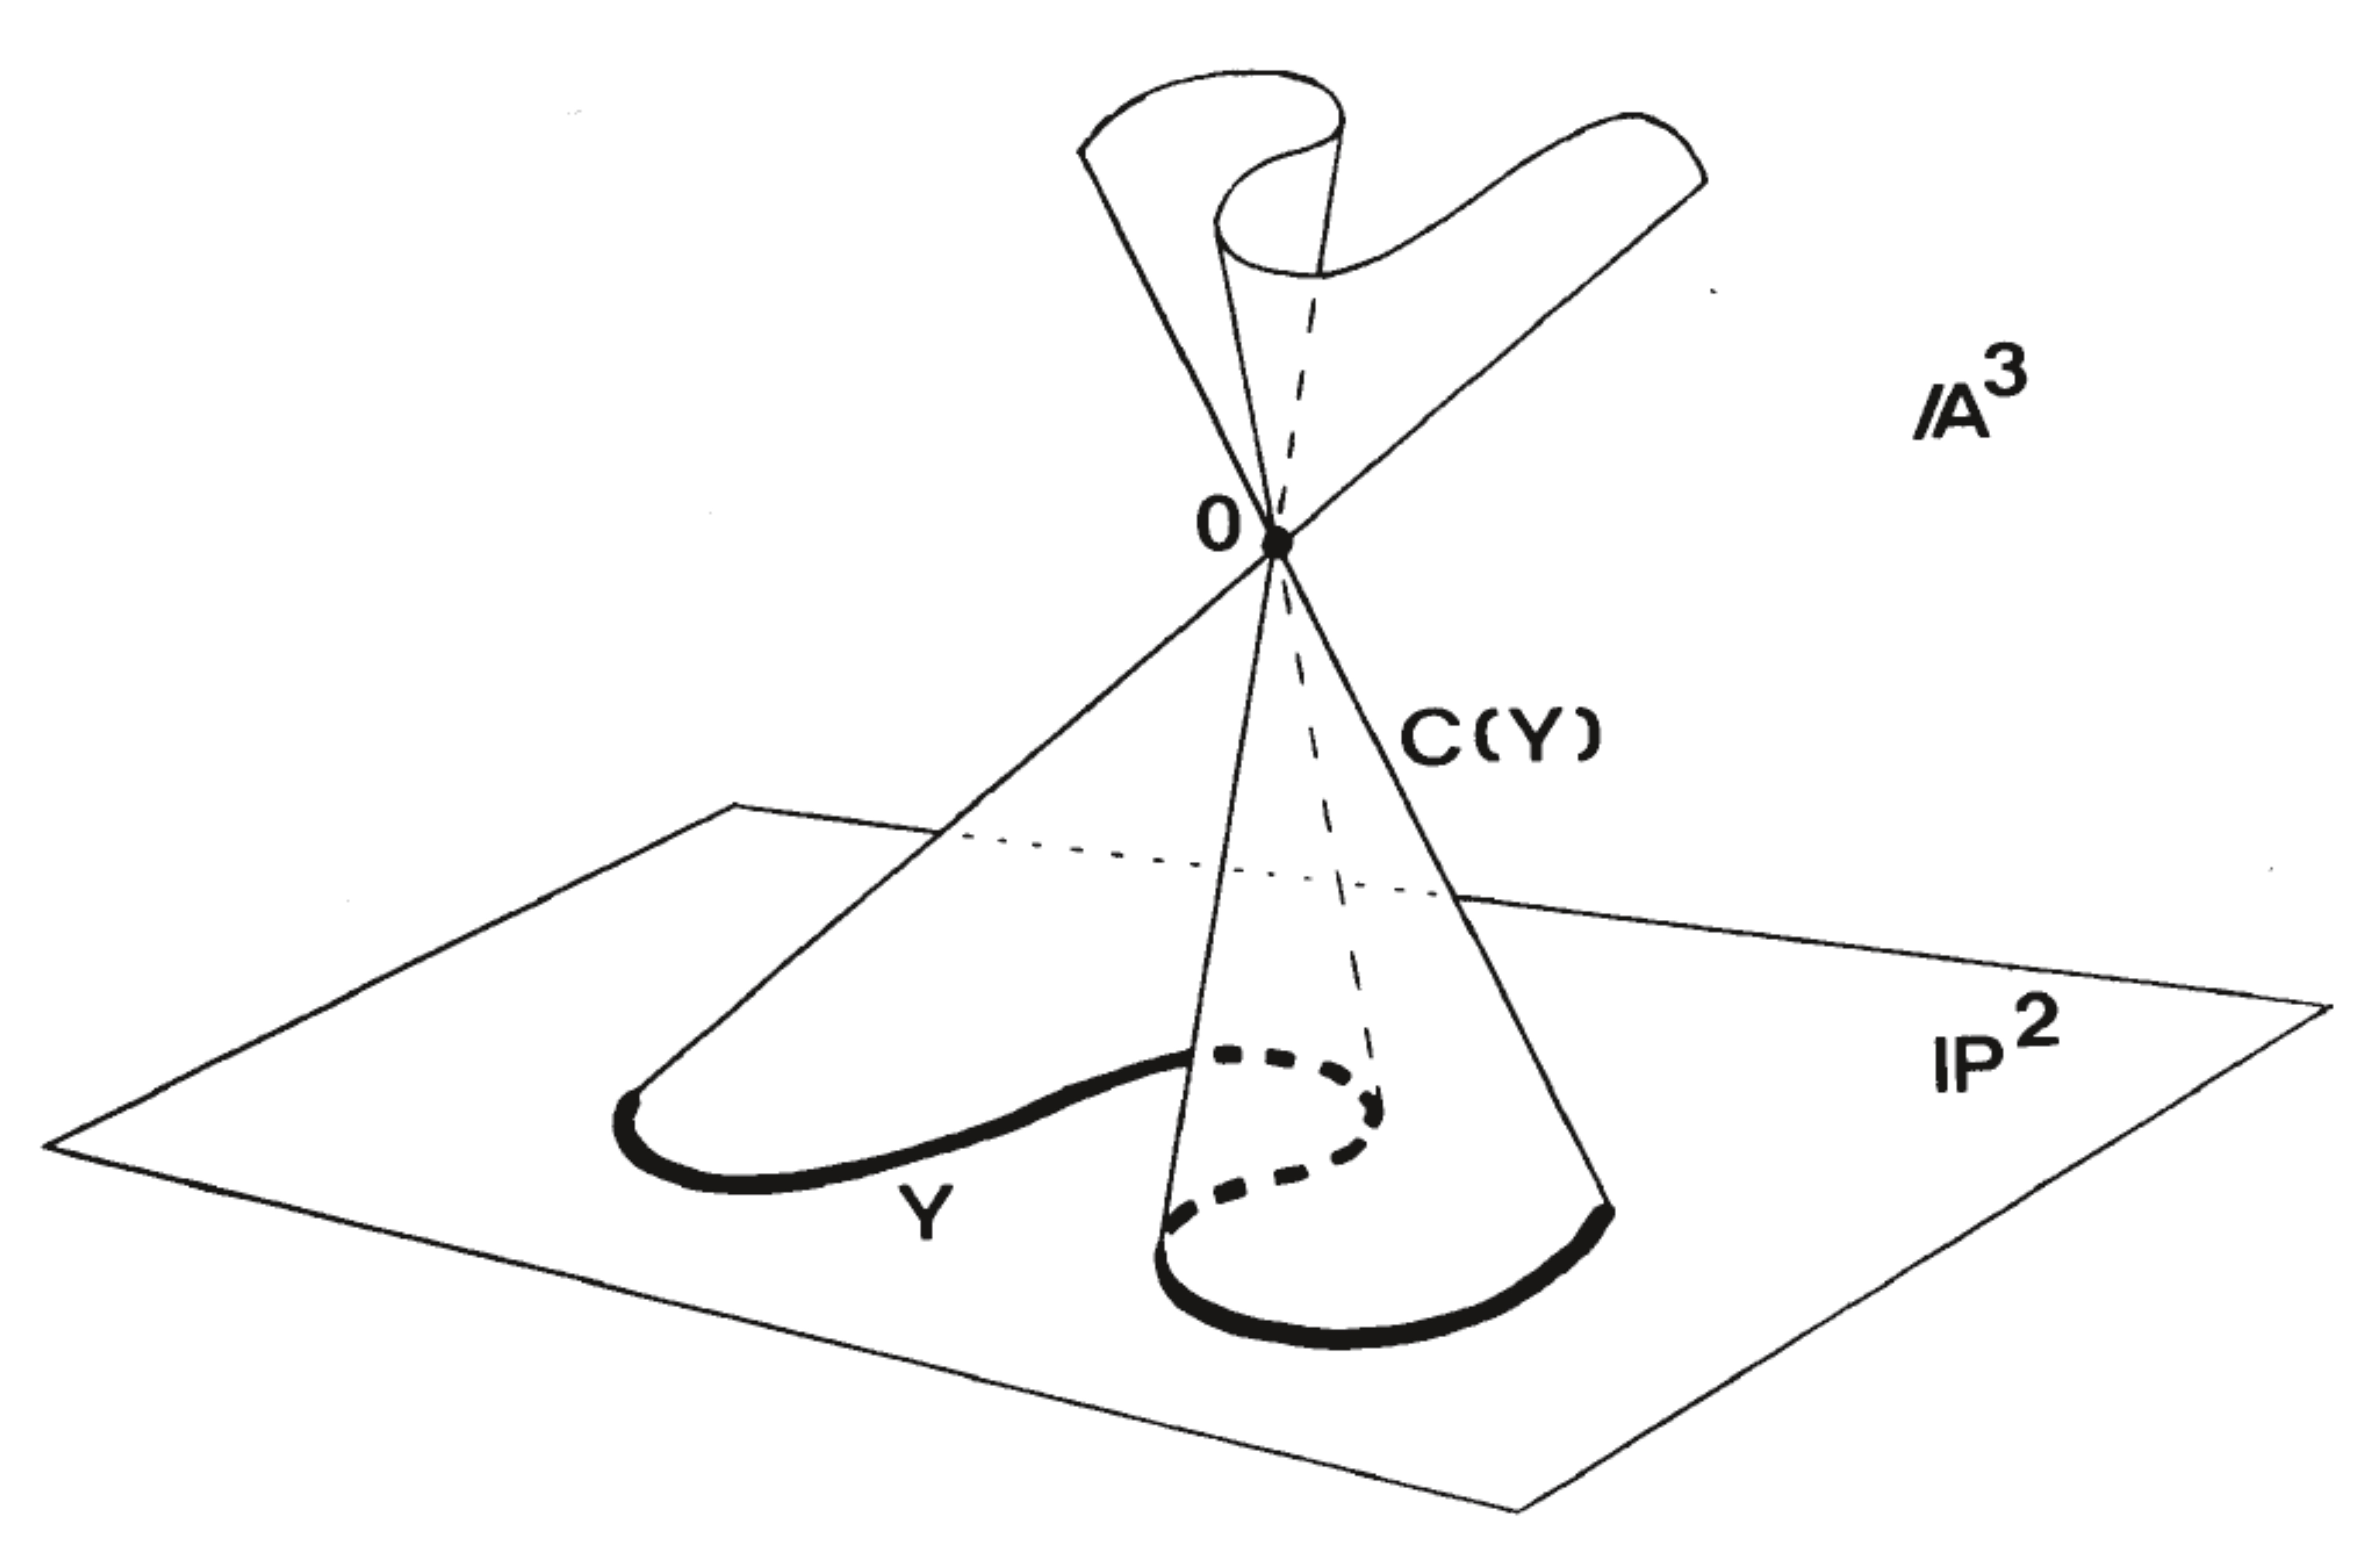
\includegraphics[width=0.5\columnwidth]{Figure1}\\
	Figure 1. $\mb P^2$에서의 곡선 상에서의 뿔
	\end{center}
	%
	\begin{enumerate}[label=,itemindent=0mm]
	\item Sol) (a) $I(Y)$가 동차 원소들에 의해 생성되므로 자명하다.\\
	(b) $C(Y)$가 기약 iff $I(Y)$가 소 아이디얼 iff $Y$가 기약.\\
	(c) $Y$가 기약일 경우 (Ex. 2.6)에 의해 $\dim Y+1=\dim S(Y)=(n+1)-\mrm{height}\:I(Y)=\dim A(C(Y))=\dim C(Y)$이다.\\
	$Y$가 기약이 아닌 경우 $Y$의 기약 성분이 $Y_1,\ldots,Y_n$이라 하자.
	$C(Y_1),\ldots,C(Y_n)$은 유한 개이고 (b)에 의해 기약이며 아핀 뿔의 정의에 의해 서로를 포함하지 않는다.
	따라서 Proposition 1.5의 유일성에 의해 이들은 $C(Y)$의 기약 성분들이다.
	각각의 $Y_i$가 기약이므로 $\dim Y_i+1=\dim C(Y_i)\:(1\le i\le n)$이 성립한다.
	$\dim Y=\max_i\dim Y_i,\dim C(Y)=\max_i\dim C(Y_i)$이므로 $\dim Y+1=\dim C(Y)$이다.\\
	\end{enumerate}
	%
	\begin{enumerate}[label=\tb{2.\arabic*.},itemindent=0mm,itemsep=4mm]
		\setcounter{enumi}{10}
		\item \tb{$\Pn$에서의 선형 대수다양체}. 1차다항식에 의해 정의된 초곡면은 \tb{초평면(hyperplane)}이라 불린다.
		\begin{enumerate}[label=(\alph*)]
			\item $\Pn$에서의 대수다양체 $Y$에 대한 다음 두 조건이 동치임을 보여라:
			\begin{enumerate}[label=(\roman*)]
				\item $I(Y)$는 1차다항식들에 의해 생성될 수 있다.
				\item $Y$는 초평면들의 교집합으로 표현될 수 있다.
			\end{enumerate}
			이 경우 우리는 $Y$가 $\Pn$에서의 \tb{선형 대수다양체(linear variety)}라 한다.
			\item 만약 $Y$가 $\Pn$에서의 $r$차원 선형 대수다양체이면
			$I(Y)$가 최소 $n-r$개의 1차다항식에 의해 생성됨을 보여라.
			\item $Y,Z$가 $\Pn$에서의 선형 대수다양체이며 $\dim Y=r,\dim Z=s$라 하자.
			만약 $r+s-n\ge 0$이면 $Y\cap Z\ne\es$이다.
			이에 더해 만약 $Y\cap Z\ne\es$이면 $Y\cap Z$는 차원 $r+s-n$ 이상의 선형 대수다양체이다.
			($\mb A^{n+1}$을 $k$ 상에서의 벡터 공간으로 간주하고 그 부분공간에서 작업하라.)
		\end{enumerate}
		\sol (a) 대수적 집합들의 교집합의 아이디얼은 아이디얼들의 합집합이다.\\
		(b) 사영공간을 아핀 열린집합 $U_i$들에 의해 덮고 (Ex. 1.9, 1.10b)를 적용하면 따라온다.\\
		(c) $\mb A^{n+1}$에서의 아핀 뿔을 고려하자. $Y$와 $Z$의 아핀 뿔은 벡터 공간으로 간주된 $\mb A^{n+1}$의
		$r+1$차원과 $s+1$차원 선형 부분공간이다. 따라서 그 교집합인 $Y\cap Z$의 아핀 뿔은
		$\mb A^{n+1}$의 $(r+1)+(s+1)-(n+1)=r+s-n+1$차원 이상의 선형 부분공간이다.
		그러므로 $Y\cap Z$는 $r+s-n$차원 이상의 선형 대수다양체이다.
		\item \tb{$d$차 매장}. 주어진 $n,d>0$에 대하여 $M_0,M_1,\ldots,M_N$이
		$n+1$개 변수 $x_0,\ldots,x_n$에 대한 모든 $d$차 단항식들이라 하자. 여기에서 $N=\binom{n+d}{n}-1$이다.
		함수 $\rho_d:\Pn\ra\mb P^N$을 점 $P=(a_0,\ldots,a_n)$을 단항식 $M_j$들에 $a_i$들을 대입하여 얻어진
		점 $\rho_d(P)=(M_0(a),\ldots,M_N(a))$로 대응시키는 함수로 정의하자.
		이는 $\Pn$에서 $\mb P^N$으로의 \tb{$d$차 매장($d$-uple embedding)}이라 불린다.
		예를 들어 만약 $n=1,d=2$이면 $N=2$이고 $\mb P^1$의 $\mb P^2$로의 $2$차 매장의 상 $Y$는 원뿔곡선이다.
		\begin{enumerate}[label=(\alph*)]
			\item $\ta:k[y_0,\ldots,y_N]\ra k[x_0,\ldots,x_n]$이
			$y_i$를 $M_i$로 대응시키는 것으로 정의된 준동형사상이며 $\mf a$가 $\ta$의 핵이라 하자.
			그 경우 $\mf a$는 동차 소 아이디얼이며 따라서 $Z(\mf a)$는 $\mb P^N$에서의 사영 대수다양체이다.
			\item $\rho_d$의 상이 정확히 $Z(\mf a)$임을 보여라. (한쪽 포함 관계는 간단하다. 반대쪽은 계산이 필요하다.)
			\item 이제 $\rho_d$가 $\Pn$에서 사영 대수다양체 $Z(\mf a)$로의 위상동형사상임을 보여라.
			\item $\mb P^3$에서의 비틀린 3차곡선(Ex. 2.9)이 적절한 좌표 선택 하에서
			$\mb P^1$의 $\mb P^3$으로의 3차 매장과 동일함을 보여라.
		\end{enumerate}
		\sol (a) $k[y_0,\ldots,y_N]$에 속한 다항식 $f$가 $\ta$에 의해 0으로 대응된다면
		$\ta$가 동차성을 보존하므로 $f$의 동차 성분들도 0의 동차 성분들, 즉 0으로 대응된다. 그러므로 $\mf a$는 동차 아이디얼이다.
		다음으로 $fg\in\mf a$이면 $\ta(fg)=\ta(f)\ta(g)=0$이며 따라서 $f$ 또는 $g$가 $\mf a$가 속한다.
		그러므로 $\mf a$는 소 아이디얼이며 $Z(\mf a)$는 사영 대수다양체이다.\\
		(b) $f\in\mf a=\ker\ta$ iff $f(M_0,\ldots,M_N)=0$이므로 $\Im\rho_d\bseq Z(\mf a)$임은 자명하다.\\
		$f\in I(\Im\rho_d)$라 하자. 그 경우 모든 $x\in\Im\rho_d$에 대하여 $f(x)=0$이며
		따라서 임의의 $(a_0,\ldots,a_n\in\Pn)$에 대하여 $f(M_0(a),\ldots,M_N(a))=0$이다.
		즉 $f(M_0,\ldots,M_N)$은 $n+1$변수 다항식이며 항등적으로 0이다.
		$k$가 무한체이므로 이는 $f(M_0,\ldots,M_N)=0$임을 함의한다.
		그러므로 $\mf a\pseq I(\Im\rho_d)$이며 $Z(\mf a)\bseq Z(I(\Im\rho_d))$이다.
		이제 $\Im\rho_d$가 $\mb P^N$에서의 Zariski 닫힌집합이며 따라서 $Z(I(\Im\rho_d))=\Im\rho_d$임을 보여야 한다.
		$\sum t_i=d$인 경우 $j(t_1,\ldots,t_n)$가 $M_{j(t_1,\ldots,t_n)}(a)=a_1^{t_1}\cdots a_n^{t_n}$을 만족시키는 수라 하자.
		또한 각각의 $i$에 대하여 $j_0(i)$를 $M_{j_0(i)}(a)=a_i^d$를 만족시키는 수로 정의하고
		$j_1(i,j)$를 $M_{j_1(i,j)}(a)=a_i^{d-1}a_j$를 만족시키는 수로 정의하자.\\
		$\Im\rho_d$가 다항식 $y_{j(t_0,\ldots,t_n)}y_{j(s_0,\ldots,s_n)}-y_{j(t'_0,\ldots,t'_n)}y_{j(s'_0,\ldots,s'_n)}
		\:(t_i+s_i=t'_i+s'_i)$들의 영점집합임을 보이자. $\Im\rho_d$의 점들이 이러한 다항식들을 만족시킴은 명백하다.
		역으로 이러한 영점집합에 속하는 임의의 점 $y_i=b_i$를 선택하자. 그 경우 모든 좌표 $b_{j_0(i)}$들이 동시에 0일 수 없다;
		이 경우 위 다항방정식들에 의해 $(b_0,\ldots,b_N)=(0,\ldots,0)$이 되어 모순이다.
		따라서 어떠한 좌표 $b_{j_0(i)}$가 0이 아니다. w.l.o.g. $b_{j_0(0)}=1$이라 하자.
		$a_0=1$로, $a_i=b_{j_1(0,i)}$로 정의하자. 그 경우 위 다항방정식들을 반복적용하면 $b_{j(t_0,\ldots,t_n)}
		=a_1^{t_1}a_2^{t_2}\cdots a_n^{t_n}=M_{j(t_0,\ldots,t_n)}(a)$를 얻는다. 따라서 이 점은 $\Im\rho_d$에 속한다.\\
		(c) 모든 좌표함수가 $d$차 동차 다항함수이므로 $\rho_d$는 Zariski 위상 하에서 연속 함수이다. (cf. Lemma 3.6)
		$\rho_d$의 역함수는 $y_{j_0(i)}\ne 0$인 조밀 열린집합 상에서 좌표 표현
		$(y_{j_1(i,0)},\ldots,y_{j_1(i,i-1)},y_{j_1(i,i+1)},\ldots,y_{j_1(l,n)})$으로 주어지므로 연속하다.
		이러한 조밀 열린 부분집합들은 $\Im\rho_d$의 덮개를 형성한다. 그러므로 이는 $\Im\rho_d$ 전체 상에서 연속하다.
		(역함수를 명시적으로 구축할 수 있으므로 $\rho_d$는 단사이다.) 따라서 $\rho_d$는 위상동형사상이다.\\
		(d) $\mb P^1$의 3차 매장은 $(x,y)\mt(x^3,x^2y,xy^2,y^3)$이다. 이는 (Ex 2.9)에서 얻은 비틀림 3차곡선의 매개변수 표현이다.
		\item $Y$가 $\mb P^2$의 $\mb P^5$로의 2차 매장의 상이라 하자. 이는 \tb{Veronese 곡면(Veronese surface)}이다.
		만약 $Z\bseq Y$가 닫힌 곡선이면(\tb{곡선(curve)}은 1차원 대수다양체이다)
		$V\cap Y=Z$를 만족시키는 초곡면 $V\bseq\mb P^5$가 존재함을 보여라.\\
		\sol $\mb P^2$의 2차 매장은 $(x,y,z)\mt(x^2,y^2,z^2,xy,yz,zx)$이다.
		2차 매장이 그 상으로의 대수다양체 동형사상이므로 (cf. (Ex. 2.13c), Section I.3)
		$Z$는 $\mb P^2$에서의 곡선으로 간주될 수 있으며 따라서 이는 $x,y,z$에 대한 동차다항식 $f$에 의해 정의된다.
		$f^2$는 짝수차 동차다항식이며 따라서 $x^2,y^2,z^2,xy,yz,zx$에 대한 다항식으로 표현 가능하다.
		(이러한 표현 방식은 유일하지 않다; 특정한 한 가지를 선택하자.
		예를 들어 각각의 항에서 $x,y,z$를 가능한 한 많이 $x^2,y^2,z^2$로 묶으면 $1$ 또는 $xy,yz,zx$ 중 정확히 하나가 남는다.)
		여기에서 변수를 $y_0,\ldots,y_5$로 대체한 다항식을 $g$라 하자.
		그 경우 $Y$의 모든 점은 $(x^2,y^2,z^2,xy,yz,zx)$로 표현되므로 $\mb P^5$에서의 $Z(g)\cap Y$는
		$\mb P^2$에서의 $Z(f^2)=Z(f)$에 대응된다. i.e. $Z(g)\cap Y=Z$가 성립한다.
		$Z$가 기약이므로 $Z(g)$의 어떠한 기약 성분 $Z(g_1)$이 존재하여 $Z(g_1)\ps Z$를 만족시킨다. 
		(여기에서 $g_1$은 $g$의 어떠한 기약 인수이다.) $Z(g_1)$이 요구된 초곡면 $V$이다.
		\item \tb{Segre 매장}. $\psi:\mb P^r\times\mb P^s\ra\mb P^N$이 순서 쌍 $(a_0,\ldots,a_r)\times(b_0,\ldots,b_s)$를
		사전 순서인 $(\ldots,a_ib_j,\ldots)$로 대응시키는 것으로 정의된 함수라 하자. 여기에서 $N=rs+r+s$이다.
		$\psi$가 잘 정의되었으며 단사임을 기억해 두라. 이는 \tb{Segre 매장(Segre embedding)}이라 불린다.
		$\psi$의 상이 $\mb P^N$의 \tb{부분대수다양체(subvariety)}임을 보여라.
		[Hint: $\mb P^N$의 동차 좌표가 $\sx{z_{ij}}{i=0,\ldots,r,j=0,\ldots,s}$라 하고
		$\mf a$가 $z_{ij}$를 $x_iy_j$로 대응시키는 준동형사상 $k[\{z_{ij}\}]\ra k[x_0,\ldots,x_r,y_0,\ldots,y_s]$의 핵이라 하자.
		그 후 $\Im\psi=Z(\mf a)$임을 보여라]\\
		\sol $f\in\mf a$ iff $f(x_0y_0,\ldots,x_ry_s)=0$이므로 (Ex. 2.12b)에서와 같은 논의에 의해 $\Im\psi=Z(\mf a)$이다.
		($\mf a$는 $z_{ij}z_{kl}-z_{kj}z_{il}$들에 의해 생성된다.)
		\item \tb{$\mb P^3$에서의 2차곡면} (Fig. 2). 방정식 $xy-zw=0$에 의해 정의된 $\mb P^3$에서의 곡면 $Q$를 고려하자.
		(\tb{곡면(surface)}은 2차원 대수다양체이다.)
		\begin{enumerate}[label=(\alph*)]
			\item $Q$가 적절한 좌표 선택 하에서 $\mb P^1\times\mb P^1$의 $\mb P^3$으로의 Segre 매장과 동일함을 보여라.
			\item $Q$가 $t\in\mb P^1$에 의해 매개화된 다음을 만족시키는 직선들의 두 개의 족 $\{L_t\},\{M_t\}$를 포함함을 보여라:
			(\tb{직선(line)}은 1차원 선형 대수다양체이다.)
			만약 $L_t\ne L_u$이면 $L_t\cap L_u=\es$, 만약 $M_t\ne M_u$이면 $M_t\cap M_u=\es$,
			모든 $t,u$에 대하여 $L_t\cap M_u=$ 한 점.
			\item $Q$가 이러한 직선들 이외에도 다른 곡선들을 포함함을 보이고 $Q$ 상에서의 Zariski 위상이
			$\mb P^1\times\mb P^1$ 상에서의 곱위상(여기에서 각각의 $\mb P^1$은 Zariski 위상을 가진다.)과
			$\psi$를 통해 위상동형이 아님을 보여라.
		\end{enumerate}
		\end{enumerate}
		%Figure 2
		\begin{center}
			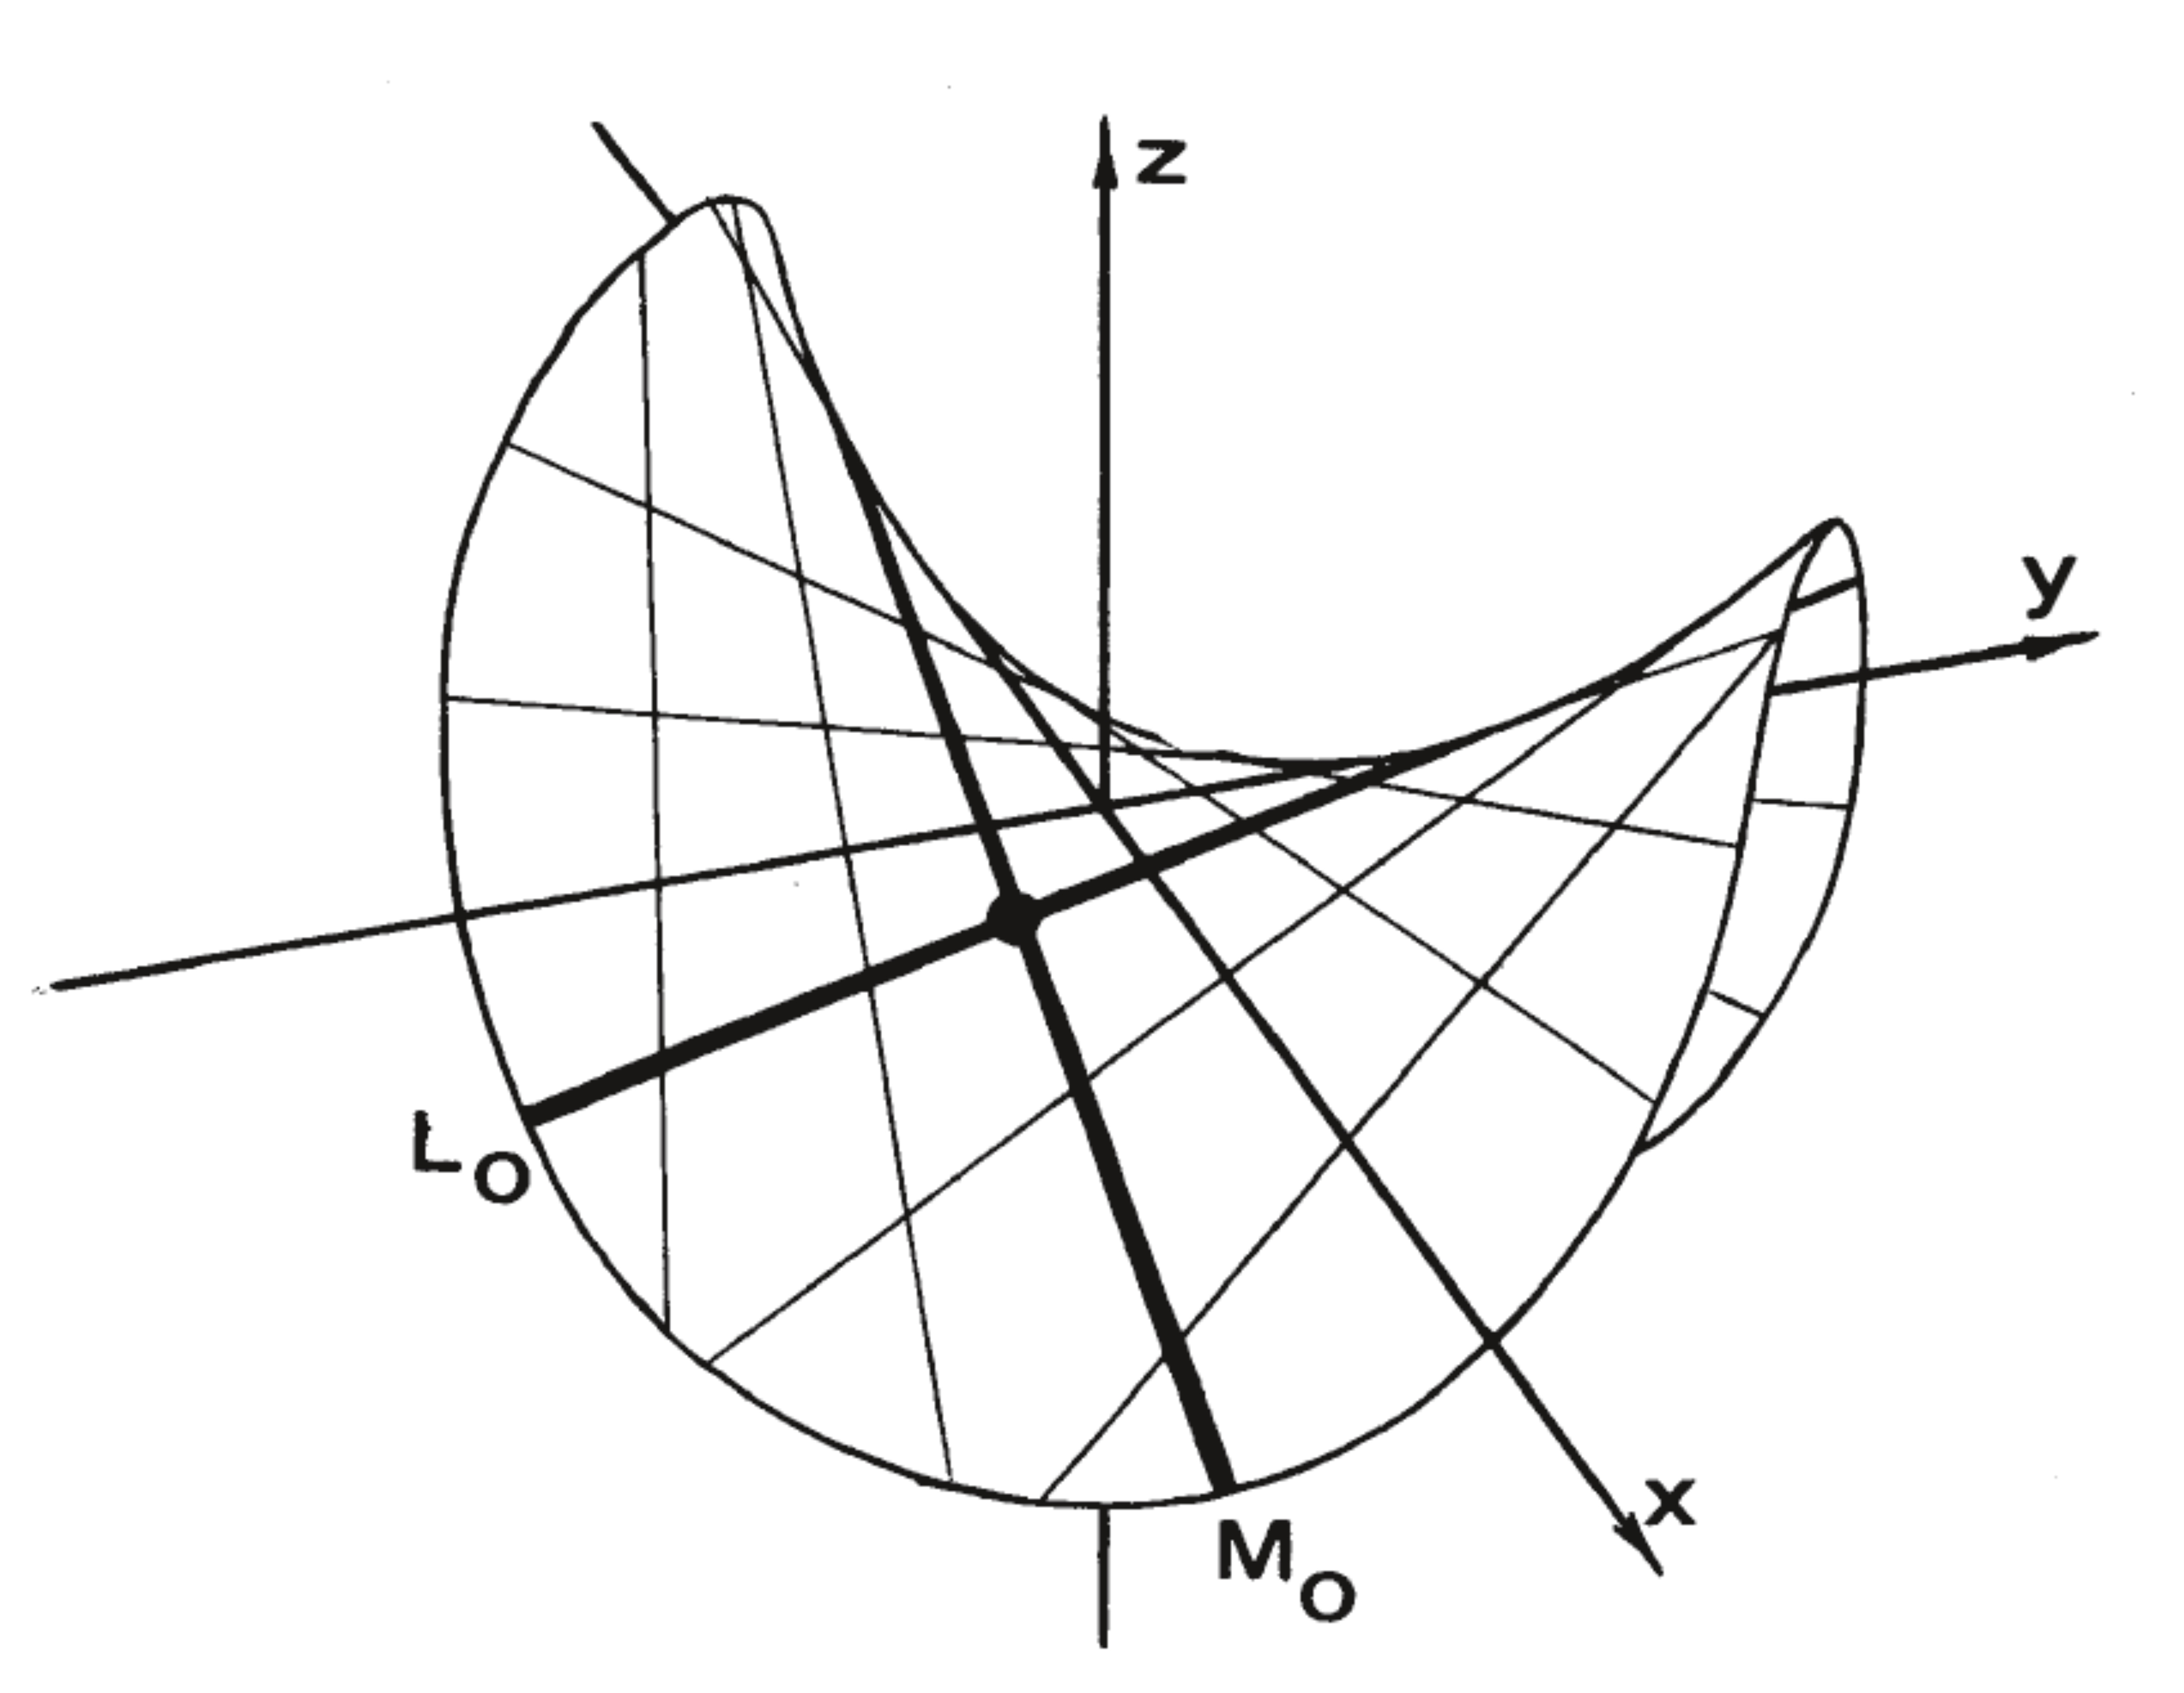
\includegraphics[width=0.5\columnwidth]{Figure2}\\
			Figure 2. $\mb P^3$에서의 2차곡면
		\end{center}
		%
		\begin{enumerate}[label=,itemindent=0mm]
		\item Sol) (a) $\mb P^1\times\mb P^1$의 Segre 매장은 $(x_0,x_1,y_0,y_1)\mt(x_0y_0,x_0y_1,x_1y_0,x_1y_1)=(w,x,y,z)$이다.
		(Ex. 2.14)에서 보였듯이 그 상의 아이디얼은 $z_{ij}z_{kl}-z_{kj}z_{il}$들에 의해 생성되며
		이들 중 자명하지 않은 원소는 $xy-zw$뿐이다. 따라서 $(xy-zw)$는 제시된 Segre 매장이다.\\
		(b) $L_t:Z(x-tz,y-tw)$ 및 $M_t:Z(x-tw,y-tz)$들이 요구된 직선이다.\\
		(c) $Q$에서는 $Z(xy-zw,x-y)$ 등 직선이 아닌 곡선도 존재한다. 그러나 Zariski 위상의 곱위상 하에서는
		모든 닫힌집합이 두 $\mb P^1$ 중 하나에 평행한 직선들의 유한 합집합이다.
		이러한 집합은 $\psi$에 의해 $Q$에서의 직선들의 유한 합집합으로 대응된다. 그러므로 이들은 위상동형이 아니다.\\
		\end{enumerate}
		\begin{enumerate}[label=\tb{2.\arabic*.},itemindent=0mm,itemsep=4mm]
		\setcounter{enumi}{15}
		\item \begin{enumerate}[label=(\alph*)]
			\item 두 대수다양체의 교집합이 대수다양체여야 할 필요는 없다.
			예를 들어 $Q_1$과 $Q_2$가 각각 방정식 $x^2-yw=0$과 $xy-zw=0$에 의해 주어진 $\mb P^3$에서의 2차곡면이라 하자.
			$Q_1\cap Q_2$가 비틀린 3차곡선과 직선의 합집합임을 보여라.
			\item 두 대수다양체의 교집합이 대수다양체이더라도 교집합의 아이디얼은 아이디얼들의 합이 아닐 수 있다.
			예를 들어 $C$가 방정식 $x^2-yz=0$에 의해 주어진 $\mb P^2$에서의 2차곡선이라 하자.
			$L$이 $y=0$에 의해 주어진 직선이라 하자. $C\cap L$이 한 점 $P$로 구성되어 있지만 $I(C)+I(L)\ne I(P)$임을 보여라.
		\end{enumerate}
		\sol (a) 아핀 열린집합 $w=1$에서 이는 $x^2-y=0,xy-z=0$이므로 이는 $(w,x,y,z)=(1,x,x^2,x^3)$인 비틀린 3차곡선이다.
		$Q_1\cap Q_2$가 닫힌집합이므로 이는 아핀 비틀린 3차곡선의 사영 폐포인 사영 비틀린 3차곡선을 포함한다.
		닫힌집합 $w=0$에서 이는 $x^2=xy=0$이므로 직선 $x=w=0$이다.\\
		(b) $C\cap L$은 한 점 $P=(0,0,z)$으로 구성된다. $x$는 $I(P)=(x,y)$에 속하지만 $I(C)+I(L)=(x^2-yz,y)$에 속하지 않는다.
		\item \tb{완비 교집합}. $\Pn$에서의 $r$차원 대수다양체 $Y$가 \tb{(강)완비 교집합((strict) complete intersection)}이라는
		것의 정의는 $I(Y)$가 $n-r$개 원소에 의해 생성될 수 있는 것이다.
		$Y$가 \tb{집합론적 완비 교집합(set-theoretic complete intersection)}이라는 것의 정의는
		$Y$가 $n-r$개 초곡면의 교집합으로 표현 가능한 것이다.
		\begin{enumerate}[label=(\alph*)]
			\item $Y$가 $\Pn$에서의 대수다양체이며 $Y=Z(\mf a)$라 하자. 또한 $\mf a$가 $q$개 원소에 의해 생성될 수 있다 하자.
			그 경우 $\dim Y\ge n-q$임을 보여라.
			\item 강완비 교집합이 집합론적 완비 교집합임을 보여라.
		\end{enumerate}
		\begin{enumerate}[label=*(\alph*)]
			\setcounter{enumii}{2}
			\item (b)의 역은 거짓이다. 예를 들어 $Y$가 $\mb P^3$에서의 비틀린 3차곡선이라 하자. (Ex. 2.9)
			$I(Y)$가 두 원소에 의해 생성될 수 없음을 보여라.
			반면에 $Y=H_1\cap H_2$를 만족시키는 각각 2차와 3차인 초곡면 $H_1,H_2$를 찾아라.
		\end{enumerate}
		\begin{enumerate}[label=**(\alph*)]
			\setcounter{enumii}{3}
			\item $\mb P^3$에서의 모든 닫힌 기약 곡선이 두 곡면의 집합론적 교집합인지는 아직 해결되지 않은 문제이다.
			해설에 대해서는 Hartshorne [1]과 Hartshorne [5, III, \S 5]를 참조하라.
		\end{enumerate}
		\sol (a) 사영공간을 아핀 열린집합 $U_i$들에 의해 덮고 (Ex. 1.9, 1.10b)를 적용하면 따라온다.\\
		(b) $Y$가 강완비 교집합이면 $I(Y)$의 $n-r$개 생성자들은 각각 초곡면을 정의하며
		$Y$는 이러한 초곡면들의 교집합이므로 집합론적 완비 교집합이다.\\
		(c) $Y=\sx{(w,x,y,z)=(t^3,t^2s,ts^2,s^3)}{t,s\in k}$이다.
		$Y$ 상에서 소멸하는 1차 동차다항식은 존재하지 않으며 $Y$ 상에서 소멸하는 2차 동차다항식은 $x^2-yw,y^2-zx,xy-zw$이다.
		이들은 서로를 생성하지 못하므로 $Y$의 아이디얼의 생성집합에는 이 세 원소가 반드시 포함되어야 한다.
		따라서 $Y$는 강완비 교집합이 아니다. 반면에 아핀 비틀린 3차곡선 $Y_0=Z(x^2-yw)\cap Z(x^3-zw^2)$(아핀 공간의 영점집합)이므로
		그 사영 폐포를 취하면 $Y=Z(x^2-yw)\cap Z(x^3-zw^2)$(사영 공간의 영점집합)이며 $Y$는 집합론적 완비 교집합이다.
	\end{enumerate}
	
	
	\subsection*{Section I.3}
	
	\begin{enumerate}[label=\tb{3.\arabic*.},itemindent=0mm,itemsep=4mm]
		\item \begin{enumerate}[label=(\alph*)]
			\item $\mb A^2$에서의 임의의 원뿔곡선이 $\mb A^1$ 또는 $\mb A^1-\{0\}$과 동형임을 보여라. (cf. Ex. 1.1)
			\item $\mb A^1$이 자신의 임의의 열린 진부분집합과 동형이 \ti{아님}을 보여라.
			(이 결과는 아래의 Ex. 6.7)에서 일반화된다.
			\item $\mb P^2$에서의 임의의 원뿔곡선은 $\mb P^1$과 동형이다.
			\item 우리는 나중에 (Ex. 4.8) 임의의 두 곡선이 위상동형임을 보일 것이다.
			그러나 $\mb A^2$는 심지어 $\mb P^2$와도 위상동형이 아님을 보여라.
			\item 만약 아핀 대수다양체가 사영 대수다양체와 동형이면 이는 한 점으로만 구성됨을 보여라.
		\end{enumerate}
		%
		\sol (a) Ex. 1.1에서 임의의 원뿔곡선 $Y$의 아핀 좌표환이 $k[x]$ 또는 $k[x,x^{-1}]$임을 보였다.
		이는 각각 $\mb A^1$과 $\mb A^1-\{0\}$의 아핀 좌표환이며 따라서 $Y$는 이들 중 하나와 동형이다.\\
		(b) $\mb A^1$의 열린 진부분집합은 $\mb A^1$에서 유한 개 점을 제외한 것이다.
		이는 평행이동에 의해 $\mb A^1-\{0,1,\ldots,n\}$과 동형이다. 이는 다시 (아핀 좌표계 $x,x_0,x_1,\ldots,x_n$을 가지는)
		$\mb A^{n+2}$에서의 초곡면 $xx_0=(x-1)x_1=(x-2)x_2=\cdots=(x-n)x_n=1$과 첫째 좌표 $x$로의 사영을 통해 동형이다.
		그 아핀 좌표환은 $k[x,x_0,x_1,\ldots,x_n]/(xx_0-1,(x-1)x_1-1,\ldots,(x-n)x_n-1)
		\cong k[x,x^{-1},(x-1)^{-1},\ldots,(x-n)^{-1}]$이다.
		그러나 이는 $\mb A^1$의 아핀 좌표환 $k[x]$와 동형이 아니므로 $\mb A^1$과 $\mb A^1-\{0,1,\ldots,n\}$은 동형이 아니다.\\
		(c) 사영평면의 원뿔곡선을 표현하는 동차다항식을 $z=1$을 대입하여 탈동차화하고 이를 Ex. 1.1에서와 같은 방식으로 변형한 후
		다시 동차화하면 다음을 얻는다: $f=x^2+axz+byz+cz^2\:(b\ne 0)$ 또는 $f=xy-z^2$.
		전자는 $ax+by+cz=-y'$으로 정의하면 $x^2-y'z$이므로 후자와 동일한 형태이다.
		따라서 사영평면의 모든 이차곡선은 $xz-y^2=0$과 동형이다.
		이는 2차 매장 $\mb P^1\ra\mb P^2$(Ex. 2.12)의 상이므로 $\mb P^1$과 동형이다. (cf. Ex. 3.4)\\
		(d) $\mb P^2$에서의 임의의 두 직선(1차원 기약 닫힌집합)은 교차하나 $\mb A^2$에서는 그렇지 않다.
		그러므로 이들은 위상동형이 아니다.\\
		(e) 아핀 대수다양체 $X$와 사영 대수다양체 $Y$가 동형이면 정칙함수환이 같아야 한다.
		$k\cong\mc O(Y)\cong\mc O(X)\cong A(X)$이므로 $X$는 한 점이다.
		%
		\item 기반 함수가 위상 공간 간의 위상동형인사상인 사상은 동형사상일 필요가 없다.
		\begin{enumerate}[label=(\alph*)]
			\item 예를 들어 $\ph:\mb A^1\ra\mb A^2$가 $t\mt(t^2,t^3)$으로 정의되었다 하자.
			$\ph$가 $\mb A^1$에서 곡선 $y^2=x^3$으로의 전단사 쌍연속 사상을 정의하지만 동형사상은 아님을 보여라.
			\item 다른 예를 위해, 기반체 $k$의 표수가 $p>0$이라 하고 함수 $\ph:\mb A^1\ra\mb A^1$을 $t\mt t^p$로 정의하자.
			$\ph$가 전단사 쌍연속이지만 동형사상은 아님을 보여라. 이는 \tb{Frobenius 사상(Frobenius morphism)}이라 불린다.
		\end{enumerate}
		%
		\sol (a) 각각의 좌표함수가 다항함수이므로 $\ph$는 대수다양체 사상이며 따라서 연속하다. 전단사임은 자명하다.
		$\ph$는 닫힌집합인 $\mb A^1$, 한 점, 공집합을 각각 $y^2=x^3$, 한 점, 공집합으로 대응시키므로 닫힌 함수이다.
		전단사 연속 닫힌 함수이므로 $\ph$는 쌍연속이며 위상동형사상이다.
		그러나 $\ph^{-1}$은 원점 근방에서 유리함수로 표현 불가하므로 대수다양체 사상이 아니며
		따라서 $\ph$가 대수다양체 동형사상이 아니다.\\
		(b) $k$가 대수적으로 닫힌 체이므로 모든 원소는 $p$제곱근을 가지며 따라서 $\ph$가 전사이다.
		$x^p-y^p=0$이면 $(x-y)^p=0$이고 $x-y=0$이므로 $\ph$가 단사이다.
		(a)에서와 같은 논의에 의해 $\ph$는 위상동형사상이지만 역함수가 유리함수로 표현 불가하므로 대수다양체 동형사상이 아니다.
		%
		\item \begin{enumerate}[label=(\alph*)]
			\item $\ph:X\ra Y$가 사상이라 하자. 그 경우 각각의 $P\in X$에 대하여
			$\ph$는 국소환의 준동형사상 $\ph_P^*:\mc O_{\ph(P),Y}\ra\mc O_{P,X}$를 유도한다.
			\item 사상 $\ph$가 동형사상일 필요충분조건은 $\ph$가 위상동형사상이며
			모든 $P\in X$에 대하여 국소환 상에 유도된 함수 $\ph_P^*$가 동형사상인 것임을 보여라.
			\item 만약 $\ph(X)$가 $Y$에서 조밀하면 모든 $P\in X$에 대하여 함수 $\ph_P^*$가 \ti{단사}임을 보여라.
		\end{enumerate}
		%
		\sol (a) $\ph_P^*:\mc O_{\ph(P),Y}\ra\mc O_{P,X}$를 $\bk{U,f}\mt\bk{\ph^{-1}(U),f\circ\ph}$로 정의하자.
		이것이 환 연산을 보존함은 자명하다.\\
		(b) ($\Ra$) $\ph$가 동형사상이면 Lemma 3.6에 의해 $\ph_P^*$들과 ${\ph^{-1}}_{\ph(P)}^*$들이 모두 환 준동형사상이다.
		이들은 서로의 역이므로 $\ph_P$가 환 동형사상이다.\\
		($\La$) $(\ph_P^*)^{-1}={\ph^{-1}}_{\ph(P)}^*$가 잘 정의됨은 $\ph^{-1}$이 대수다양체 사상임을 함의한다.\\
		(c) $\ph^*:f\mt f\circ\ph$로 정의하자. $\ph^*(f)=0$이라 가정하자. 그 경우 어떠한 근방 $\ph(U)\bs Y$ 상에서 $f=0$이다.
		만약 $f\ne 0$이면 $\ph(X)\bseq Z(f)\bsneq Y$이며 $\ph(X)$의 조밀성에 모순이다.
		%
		\item $\Pn$의 $d$차 매장(Ex. 2.12)가 그 상으로의 동형사상임을 보여라.\\
		%
		\sol $d$차 매장 $\rho_d$의 모든 좌표가 동차 다항함수이므로 $\rho_d$는 대수다양체 사상이다.
		각각의 $i$에 대하여 $j_0(i)$를 $M_{j_0(i)}(a)=a_i^d$를 만족시키는 수로 정의하고
		$j_1(i,j)$를 $M_{j_1(i,j)}(a)=a_i^{d-1}a_j$를 만족시키는 수로 정의하자.
		$\rho_d$의 역함수는 $y_{j_0(i)}\ne 0$인 조밀 열린집합 상에서 좌표 표현\\
		$(y_{j_1(i,0)},\ldots,y_{j_1(i,i-1)},y_{j_1(i,i+1)},\ldots,y_{j_1(l,n)})$으로 주어진다.
		이러한 조밀 열린 부분집합들은 $\Im\rho_d$의 덮개를 형성한다. 따라서 $\rho_d$는 대수다양체 동형사상이다.
		%
		\item 언어를 남용하여 대수다양체가 `아핀'이라는 것을 아핀 대수다양체와 동형인 것이라 하겠다.
		만약 $H\bseq\Pn$이 임의의 초곡면이면 $\Pn-H$가 아핀임을 보여라. [Hint: $H$가 $d$차라 하자.
		$\Pn$의 $\mb P^N$으로의 $d$차 매장을 고려하고 $\mb P^N$에서 초평면을 제외한 것이 아핀이라는 사실을 사용하라.]\\
		%
		\sol $\Pn-H$의 $d$차 매장의 상은 $\Pn$의 상과 $H$를 정의하는 다항식의 계수들에 의해 결정된 $\mb P^N$에서의 초평면의 차집합이다.
		$\mb P^N$에서 초평면을 제외한 것이 아핀이므로 그 닫힌 부분집합인 $\Pn-H$의 상도 아핀이다.
		(Ex. 3.4)에 의해 $d$차 매장이 그 상으로의 동형사상이므로 $\Pn-H$가 아핀이다.
		%
		\item 아핀이 아닌 준아핀 대수다양체가 존재한다. 예를 들어 $X=\mb A^2-\{0,0\}$가 아핀이 아님을 보여라.
		[Hint: $\mc O(X)\cong k[x,y]$임을 보이고 (3.5)를 사용하라. 다른 증명을 위해서는 (III, Ex. 4.3)을 참조하라.]\\
		%
		\sol 하나의 2차다항식이 $\{(0,0)\}$에서만 영점을 가질 수는 없다.
		따라서 $f=g/h$ 형태의 기약분수 표현에서 $h=1$이어야 하며 $\mc O(X)\cong k[x,y]$이다.
		$\mb A^2-\{(0,0)\}$이 아핀 대수다양체라 가정하자. $X=\mb A^2,Y=\mb A^2-\{(0,0)\}$에 대하여 Proposition 3.5을 적용하자.
		$k[x,y]$의 항등사상에 대응하는 사상은 $\mb A^2$의 항등사상이다.
		그러나 그 상은 $\mb A^2-\{(0,0)\}$에 포함되지 않으므로 모순이다.
		%
		\item \begin{enumerate}[label=(\alph*)]
		\item $\mb P^2$에서의 임의의 두 곡선이 공집합이 아닌 교집합을 가짐을 보여라.
		\item 더 일반적으로, $Y\bseq\Pn$이 1차원 이상의 사영 대수다양체이며 $H$가 초곡면이면 $Y\cap H\ne\es$임을 보여라.
		[Hint: (Ex. 3.5)와 (Ex. 3.1e)를 사용하라. 일반화를 위해서는 (7.2)를 참조하라.]
		\end{enumerate}
		%
		\sol (b) $Y\cap H=\es$이면 $Y\bseq\Pn-H$이며 (Ex. 3.5)에 의해 $\Pn-H$가 아핀이므로 $Y$도 아핀이다.
		$Y$가 아핀이며 사영이므로 (Ex. 3.1e)에 의해 한 점이다. 이는 1차원 이상임에 모순이다.
		(a)는 (b)의 특수한 경우이다.
		%
		\item $H_i$와 $H_j$가 $x_i=0$과 $x_j=0\:(i\ne j)$에 의해 정의된 $\Pn$에서의 초평면이라 하자.
		$\Pn-(H_i\cap H_j)$ 상에서의 임의의 정칙 함수가 상수함수임을 보여라.
		(이는 $Y=\Pn$인 경우에 대하여 (3.4a)의 다른 증명을 제공한다.)\\
		%
		\sol $\Pn-H_i$에서의 정칙 함수들은 $x_i$를 제외한 $n$개 변수에 대한 다항식의 $x_i$에 의한 동차화를
		같은 차수 $n$을 가지는 $x_i^n$으로 나눈 것이다. $\Pn-H_j$에서도 마찬가지이다.
		$\Pn-(H_i\cap H_j)$에서의 정칙 함수들은 동시에 $\Pn-H_i$와 $\Pn-H_j$에서 정칙이므로
		분모가 $x_i$의 멱이며 동시에 $x_j$의 멱이다. 그러므로 분모가 0차이며 따라서 분자도 0차이고 그러므로 상수함수이다.
		%
		\item 사영 대수다양체의 동차 좌표환은 동형 하에서 불변이 아니다.
		예를 들어 $X=\mb P^1$이라 하고 $Y$가 $\mb P^1$의 $\mb P^2$로의 2차 매장이라 하자.
		그 경우 $X\cong Y$(Ex. 3.4)이다. 그러나 $S(X)\not\cong S(Y)$임을 보여라.\\
		%
		\sol
		%
		\item \tb{부분대수다양체.} 위상공간의 부분집합이 \tb{국소 닫혀 있다(locally closed)}는 것의 정의는
		그 폐포 내에서 열린 부분집합인 것이다. 또는 이와 동치로 열린집합과 닫힌집합의 교집합인 것이다.\\
		만약 $X$가 준아핀 또는 준사영 대수다양체이며 $Y$가 기약 국소 닫힌 부분집합이라 하자.
		그 경우 $Y$도 동일한 아핀 또는 사영공간의 국소 닫힌 부분집합이 되므로 준아핀(resp. 준사영) 대수다양체이다.
		우리는 이를 $Y$ 상에서의 \tb{유도 구조(induced structure)}라 부르며 $Y$가 $X$의 \tb{부분대수다양체(subvariety)}라 한다.\\
		이제 $\ph:X\ra Y$가 사상이며 $X'\bseq X$와 $Y'\bseq Y$가 $\ph(X')\bseq Y'$을 만족시키는 기약 국소 닫힌 부분집합이라 하자.
		$\ph\rest_{X'}:X'\ra Y'$이 사상임을 보여라.\\
		%
		\sol
		%
		\item $X$가 임의의 대수다양체이며 $P\in X$라 하자.
		국소환 $\mc O_P$의 소 아이디얼과 $P$를 포함하는 $X$의 닫힌 부분대수다양체 간에 일대일 대응이 존재함을 보여라.\\
		%
		\sol
		%
		\item 만약 $P$가 대수다양체 $X$ 상의 점이면 $\dim\mc O_P=\dim X$이다. [Hint: 아핀 경우로 문제를 줄이고 (3.2c)를 사용하라.]\\
		%
		\sol
		%
		\item \tb{부분대수다양체의 국소환.} $Y\bseq X$가 부분대수다양체라 하자.
		$\mc O_{Y,X}$가 $U\cap Y\ne\es$인 열린집합 $U\bseq X$와 $U$ 상에서의 정칙 함수 $f$의 동치류 $\bk{U,f}$들의 집합이라 하자.
		$\bk{U,f}$가 $\bk{V,g}$와 동치임을 $U\cap V$ 상에서 $f=g$인 것으로 정의한다.
		$\mc O_{Y,X}$가 국소환이며 잉여류체 $K(Y)$를 가지고 차원이 $\dim X-\dim Y$임을 보여라.
		이는 $Y$의 $X$ 상에서의 \tb{국소환(local ring)}이다.
		만약 $Y=P$가 점이면 $\mc O_P$를 얻으며 $Y=X$이면 $K(X)$를 얻음을 기억해 두라.
		또한 만약 $Y$가 점이 아니면 $K(Y)$는 대수적으로 닫혀 있지 않으며
		따라서 이러한 방식으로 얻는 국소환들은 대수적으로 닫혀 있지 않은 잉여류체를 가진다.\\
		%
		\sol
		%
		\item \tb{한 점에서의 사영.} $\Pn$이 $\mb P^{n+1}$에서의 초평면이며 $P\in\mb P^{n+1}-\Pn$이라 하자.
		함수 $\ph:\mb P^{n+1}-\{P\}\ra\Pn$을 $\ph(Q)=P$와 $Q$를 포함하는 유일한 직선과 $\Pn$의 교집합으로 정의하자.
		\begin{enumerate}[label=(\alph*)]
		\item $\ph$가 사상임을 보여라.
		\item $Y\bseq\mb P^3$이 비틀린 3차곡선이라 하자. 이는 $\mb P^1$의 3차 매장의 상이다. (Ex. 2.12)
		만약 $t,u$가 $\mb P^1$ 상에서의 동차 좌표계이면 $Y$가 \tb{매개변수에 의해(parametrically)}
		$(x,y,z,w)=(t^3,t^2u,tu^2,u^3)$로 주어졌다고 한다. $P=(0,0,1,0)$이며 $\mb P^2$가 초평면 $z=0$이라 하자.
		$Y$의 $P$에서의 사영이 평면에서의 첨점을 가지는 3차곡선임을 보이고 그 방정식을 찾아라.
		\end{enumerate}
		%
		\sol (a) 좌표변환을 통해 $\Pn$이 $x_0=0$에 의해 정의되었으며 $P=(1,0,\ldots,0)$이라 하자.
		$Q=(x_0,x_1,\ldots,x_{n+1})\in\mb P^{n+1}-\{P\}$라 하면 $\ph(Q)=(0,x_1,\ldots,x_{n+1})$이다. 따라서 $\ph$는 사상이다.\\
		(b) 사영 $(t^3,t^2u,u^3)$의 점들은 $x^2z-y^3$의 영점이다.
		$x^2z-y^3$의 모든 영점이 $(t^3,t^2u,u^3)$ 형태임을 보이자.
		$x,y,z$ 중 0인 좌표가 존재하는 경우는 $(0,0,1)$ 또는 $(1,0,0)$뿐이며 각각 $t=0,u=1$과 $t=1,u=0$에 해당한다.
		그렇지 않은 경우 $x$의 임의의 3승근을 $t$로 설정하고 $u=ty/x$로 설정하면
		$t^3=x,t^2u=t^3y/x=y,u^3=t^3y^3/x^3=y^3/x^2=z$가 되므로 이러한 $t$와 $u$는 $(x,y,z)$를 표현한다.
		따라서 사영은 $x^2z-y^3$의 영점집합이며 이는 평면에서의 첨점을 가지는 3차곡선이다.
		%
		\item \tb{아핀 대수다양체의 곱.} $X\bseq\An$과 $Y\bseq\mb A^m$이 아핀 대수다양체라 하자.
		\begin{enumerate}[label=(\alph*)]
		\item $X\times Y\bseq\mb A^{n+m}$이 유도 위상 하에서 기약임을 보여라.
		[Hint: $X\times Y$가 닫힌 부분집합들의 합집합 $Z_1\cup Z_2$라 가정하자.
		$X_i=\sx{x\in X}{x\times Y}\bseq Z_i,i=1,2$라 하자. $X=X_1\cup X_2$이며 $X_1,X_2$가 닫힌집합임을 보여라.
		그 경우 $X=X_1$ 또는 $X_2$이며 따라서 $X\times Y=Z_1$ 또는 $Z_2$이다.]
		아핀 대수다양체 $X\times Y$는 $X$와 $Y$의 \tb{곱(product)}이라 불린다.
		그 위상이 일반적으로 곱위상과 같지 않음을 기억해 두라. (Ex. 1.4)
		\item $A(X\times Y)\cong A(X)\otimes_kA(Y)$임을 보여라.
		\item $X\times Y$가 대수다양체의 범주에서의 곱임을 보여라. i.e. (i) 사영 $X\times Y\ra X$와 $X\times Y\ra Y$가 사상이며
		(ii) 주어진 대수다양체 $Z$와 사상 $Z\ra X,Z\ra Y$에 대하여 유일한 사상 $Z\ra X\times Y$가 존재하여
		다음의 도표가 가환이도록 한다.
		%
		$$\begin{tikzcd}[row sep=large]Z\arrow[rr]\arrow[dr]\arrow[drrr]&&X\times Y\arrow[dl]\arrow[dr]\\&X&&Y\end{tikzcd}$$
		%
		\item $\dim X\times Y=\dim X+\dim Y$임을 보여라.
		\end{enumerate}
		%
		\sol (a) $X\times Y=Z_1\cup Z_2$이며 $Z_i$들이 닫힌집합이라 하고 $X_i=\sx{x\in X}{x\times Y}\bseq Z_i$라 정의하자.
		$Y$가 기약이므로 $X=X_1\cup X_2$이다. $X_i=\pr_1(Z_i)$이므로 닫힌집합이다.
		$X$가 기약이므로 $X=X_1$ 또는 $X=X_2$이며 따라서 $X\times Y=Z_1$ 또는 $Z_2$이다. 그러므로 $X\times Y$는 기약이다.\\
		(b) 준동형사상 $\ph:A(X)\otimes_kA(Y)\ra A(X\times Y)$를 $(\sum f_i\otimes g_i)(x,y)=\sum f_i(x)g_i(y)$이도록 정의하자.
		우변은 $X\times Y$ 상에서의 정칙 함수이다. $\ph$의 상에 좌표함수들이 포함되므로 $\ph$는 전사이다.
		$\ph$가 단사임을 보이기 위해서는 $f_i$들이 $A(X)$에서 선형 독립이며 $g_j$들이 $A(Y)$에서 선형 독립이면
		$f_i\otimes g_j$들이 $A(X\times Y)$에서 선형 독립임을 보이면 충분하다:
		만약 $\sum_{i,j}c_{ij}f_i(x)g_y(j)=0$이면 $f_i$들의 선형 독립성에 의해 임의의 $i$와 임의의 고정된 $y$에 대하여
		$\sum_jc_{ij}g_j(y)=0$이며 $g_j$들의 선형 독립성에 의해 모든 $c_{ij}=0$이다.\\
		(c) 사영이 사상임은 자명하다. $\ph:Z\ra X$와 $\psi:Z\ra Y$가 주어진 경우 유일한 사상
		$\ph\times\psi:Z\ra X\times Y,z\mt(\ph(z),\psi(z))$가 존재하여 사영과의 합성이 원래 사상이도록 한다.\\
		(d) $\dim X=n,\dim Y=m$이라 하자. $X$와 $Y$의 좌표들을 각각 $x_i,y_j$들이라 하자.
		$A(X\times Y)$는 모든 $x_i$들과 $y_j$들에 의해 생성된다. 이들이 대수적 독립임을 보이면 충분하다.
		$X\times Y$ 상에서 $f(x_1,\ldots,x_n,y_1,\ldots,y_m)=0$이라 하자.
		$x$를 고정하면 $y_j$들로 구성된 항들의 계수 $a_k(x)$들이 존재한다. $y_j$들의 대수적 독립성에 의해 모든 $a_k(x)=0$이다.
		그러므로 $f=0$이며 모든 좌표가 대수적 독립이다. 따라서 $\dim X\times Y=n+m$이다.
		%
		\item \tb{준사영 대수다양체의 곱.} Segre 매장(Ex. 2.14)을 사용하여 $\Pn\times\mb P^m$을 그 상과 동일시하고
		따라서 사영 대수다양체 구조를 부여하자. 이제 임의의 두 준사영 대수다양체 $X\bseq\Pn$과 $Y\bseq\mb P^m$에 대하여
		$X\times Y\bseq\Pn\times\mb P^m$을 고려하자.
		\begin{enumerate}[label=(\alph*)]
		\item $X\times Y$가 준사영 대수다양체임을 보여라.
		\item 만약 $X,Y$가 모두 사영이면 $X\times Y$도 사영임을 보여라.
		\end{enumerate}
		\begin{enumerate}[label=*(\alph*)]
		\setcounter{enumii}{2}
		\item $X\times Y$가 대수다양체의 범주에서의 곱임을 보여라.
		\end{enumerate}
		%
		\sol (b) $\Pn\times\mb P^m$에서의 사영을 고려하자.
		사영이 연속하므로 사영 대수다양체 $X$의 역상 $X\times\mb P^m$과 $Y$의 역상 $\Pn\times Y$가 닫힌집합이고
		그 교집합 $X\times Y$도 닫힌집합이다. (Ex. 3.15a)에서와 같은 논의에 의해 $X\times Y$가 기약이므로 사영 대수다양체이다.]\\
		(a) (b)에 의해 $\bar X\times\bar Y$가 사영 대수다양체이며 (b)에서와 유사한 논의에 의해 $X\times Y$는 이곳에서의 열린집합이다.
		i.e. $X\times Y$가 준사영 대수다양체이다.\\
		(c) $X$와 $Y$의 아핀 열린 덮개를 $\{X_i\},\{Y_j\}$라 하고 $Z_{ij}=\pr_1^{-1}(X_i)\cap\pr_2^{-1}(Y_j)$라 하자.
		(Ex. 3.15c)에 의해 가환 도표를 만족시키는 사상 $\phi_{ij}:Z_{ij}\ra X_i\times Y_j$가 존재한다.
		이들이 교집합 상에서 서로 호환되며 따라서 이어붙여져 사상 $Z\ra X\times Y$를 형성함을 보여야 한다.
		임의의 첨자 $i,i',j,j'$을 고정하자. 대수다양체 $X_i\cap X_{i'}$와 $Y_j\cap Y_{j'}$의
		임의의 아핀 열린집합 $X',Y'$을 고정하자;
		(Ex. 3.15c)의 유일성을 적용하면 $\pr_1^{-1}(X')\cap\pr_2^{-1}(Y')$ 상에서 $\phi_{ij}=\phi_{i'j'}$임을 얻는다.
		따라서 유일한 사상 $\phi:Z\ra X\times Y$가 존재하여 가환 도표를 만족시킨다.
		%
		\item \tb{정규 대수다양체.} 대수다양체 $Y$가 \tb{점 $P\in Y$에서 정규(normal at a point $P\in Y$)}라는 것의 정의는
		$\mc O_P$가 정수적으로 닫힌 환인 것이다. $Y$가 \tb{정규(normal)}라는 것의 정의는 모든 점에서 정규인 것이다.
		\begin{enumerate}[label=(\alph*)]
		\item $\mb P^2$에서의 모든 원뿔곡선이 정규임을 보여라.
		\item 방정식 $Q_1:xy=zw$와 $Q_2:xy=z^2$에 의해 주어진 $\mb P^3$에서의 2차곡면 $Q_1,Q_2$가 정규임을 보여라.
		(cf. 후자에 대하여 (II. Ex. 6.4))
		\item $\mb A^2$에서의 첨점을 가지는 3차곡선 $y^2=x^3$이 정규가 아님을 보여라.
		\item 만약 $Y$가 아핀이면 $Y$가 정규일 필요충분조건은 $A(Y)$가 정수적으로 닫혀 있는 것이다.
		\item $Y$가 아핀 대수다양체라 하자. 정규 아핀 대수다양체 $\bar Y$와 사상 $\pi:\bar Y\ra Y$가 존재하여
		$Z$가 정규 대수다양체이며 $\ph:Z\ra Y$가 \tb{우세(dominant)}(i.e. $\ph(Z)$가 $Y$에서 조밀) 사상이면
		유일한 사상 $\ta:Z\ra\bar Y$가 존재하여 $\ph=\pi\circ\ta$를 만족시키는 성질을 가진다.
		$\bar Y$는 $Y$의 \tb{정규화(normalization)}라 불린다. 위의 (3.9A)가 필요할 것이다.
		\end{enumerate}
		%
		\sol 정칙 국소환이 정수적으로 닫혀 있으므로 비특이 대수다양체는 정규이다.\\
		(a) (Ex. 3.1c)에 의해 원뿔곡선은 $\mb P^1$과 동형이며 $\mb P^1$이 비특이이다.\\
		(b) $Q_1$은 $\mb P^1\times\mb P^1$의 Segre 매장 하에서의 상이다. $\mb P^1\times\mb P^1$이 비특이이므로 $Q_1$이 정규이다.
		$Q_2$는 1차다항식에 의한 좌표변환을 통해 $x^2+y^2-z^2=0$으로 변환될 수 있다. (cf. Ex. 3.1)
		이는 유일한 특이점 $(0,0,0,1)$을 가진다. 따라서 아핀 열린집합 $w=1$에서 정규성을 확인하면 충분하다.\\
		i) $\Char k\ne 2$인 경우.
		$A(X)=\sx{u+vz}{u,v\in k[x,y]}$가 분수체 $K(X)=\sx{u+vz}{u,v\in k(x,y)}$에서 정수적으로 닫혀 있음을 보이면 충분하다.
		(cf. (d)) $A(X)$는 $k[x,y]$ 상에서의 유한생성 모듈이며 따라서 $A(X)$의 모든 원소가 $k[x,y]$ 상에서 정수적이다.
		만약 $\al=u+vz\in K(X)$가 $A(X)$ 상에서 정수적이면 이는 $k[x,y]$ 상에서도 정수적이어야 한다.
		그 최소다항식은 $\msf T^2-2u\msf T+u^2-(x^2+y^2)v^2$이며 따라서 $2u\in k[x,y]$이고 $u\in k[x,y]$여야 한다.
		마찬가지로 $(x^2+y^2)v^2\in k[x,y]$이다. $\Char k\ne 2$이므로 $x^2+y^2=(x+\sqrt{-1}y)(x-\sqrt{-1}y)$가
		서로 소 기약다항식의 곱이며 그러므로 $v\in k[x,y]$이고 따라서 $\al\in A(X)$이다.
		ii) $\Char k=2$인 경우. 정의하는 다항식이 $(x+y+z)^2=0$이므로 $A(X)=k[x,y]$이다. 이는 자명하게 정수적으로 닫혀 있다.\\
		(c) Theorem 6.2에 의해 1차원 Noether 국소 정역이 정칙 국소환임과 정수적으로 닫혀 있음은 동치이며
		따라서 $y^2=x^3$은 특이점을 가지므로 정규가 아니다.\\
		(d) 정역이 정수적으로 닫혀 있음은 모든 극대 아이디얼에서의 국소화가 정수적으로 닫혀 있음과 동치이다.\\
		(e) $A(\bar Y)$가 $A(Y)$의 $K(Y)$에서의 정수적 폐포라 하자.
		Theorem 3.9A에 의해 이는 동형 하에서 유일한 아핀 대수다양체 $\bar Y$를 정의한다. (d)에 의해 $\bar Y$는 정규이다.
		우세 사상 $\ph:Z\ra Y$는 함수체의 매장 $\ph^*:K(Y)=K(\bar Y)\hra K(Z),f\mt f\circ\ph$를 유도한다.
		$A(Z)$가 정수적으로 닫혀 있으므로 $\ph^*$의 $A(\bar Y)$로의 제한은 준동형사상 $A(\bar Y)\ra A(Z)$를 유도한다.
		이를 다시 $A(Y)$로 제한하면 다음과 같은 가환 도표가 성립한다.
		%
		$$\begin{tikzcd}A(Y)\arrow[r,hookrightarrow]\arrow[dr,swap,"\ph^*"]&A(\bar Y)\arrow[d,"\ph^*"]\\&A(Z)\end{tikzcd}$$
		%
		아핀 대수다양체의 범주는 정역인 유한생성 대수들의 범주와 반변 동치이므로
		대응하는 아핀 대수다양체에 대한 반대 화살표를 가진 가환 도표를 만족시키는 사상이 존재한다.
		%
		\item \tb{사영적 정규 대수다양체.} 사영 대수다양체 $Y\bseq\Pn$이 (주어진 매장에 대하여)
		\tb{사영적 정규(projectively normal)}라는 것의 정의는 그 동차 좌표환 $S(Y)$가 정수적으로 닫혀 있는 것이다.
		\begin{enumerate}[label=(\alph*)]
		\item $Y$가 사영적 정규이면 $Y$는 정규이다.
		\item 사영적 정규가 아닌 사영공간에서의 정규 대수다양체가 존재한다.
		예를 들어 $Y$가 매개변수에 의해 $(x,y,z,w)=(t^4,t^3u,tu^3,u^4)$에 의해 주어진 $\mb P^3$에서의 비틀린 4차곡선이라 하자.
		그 경우 $Y$는 정규이지만 사영적 정규가 아니다. 더 많은 예를 위해서는 (III, Ex. 5.6)을 참조하라.
		\item $Y$에서의 비틀린 4차곡선이 사영적 정규 곡선 $\mb P^1$과 동형임을 보여라. 따라서 사영적 정규성은 매장에 의존한다.
		\end{enumerate}
		%
		\sol (a) $Y$가 사영적 정규라 가정하자. i.e. $S(Y)$가 닫혀 있다. $S(Y)$의 분수체를 $Q=S(Y)_{(0)}$로 표기하자.
		임의의 점 $P\in Y$를 고정하고 $P$에 대응하는 극대 아이디얼을 $\mf m_P$라 하자.
		정수적으로 닫힌 정역의 극대 아이디얼에서의 국소화도 정수적으로 닫혀 있으므로 $S(Y)_{\mf m_P}$가 ($Q$에서) 정수적으로 닫혀 있다.
		$Q$와 그 부분환 $S(Y)_{\mf m_P}$는 $S(Y)$의 등급으로부터 유도된 자연스러운 정수 등급을 가진다.
		$Q$의 임의의 0급 원소 $b$는 $S(Y)_{\mf m_P}$ 상에서 정수적이므로
		최소다항식 $b^n+a_{n-1}b^{n-1}+\cdots+a_0=0,a_i\in S(Y)_{\mf m_P}$를 가질 것이다.
		여기에서 모든 $a_i$들을 자신의 0급항으로 대체해도 방정식이 성립한다.
		이는 모든 $b\in Q_0=S(Y)_{((0))}\cong K(Y)$가 $S(Y)_{(\mf m_P)}=\mc O_P$ 상에서 정수적임을 보여준다.
		i.e. 국소환 $\mc O_P$가 정수적으로 닫혀 있다.\\
		(b) $\mb P^3$ 비틀린 4차곡선 $Y$는 $\mb P^1$의 하나의 항 $t^2u^2$가 제외된 4차 매장 하에서의 상이다.
		$d$차 매장이 동형사상임을 보인 것과 동일한 방법으로 이것 또한 동형사상임을 보일 수 있다. $\mb P^1$이 정규이므로 $Y$도 정규이다.
		그러나 $S(Y)\cong k[t^4,t^3u,tu^3,u^4]$는 정수적으로 닫혀 있지 않다;
		$t^2u^2\in K(Y)$는 $\msf T^2-t^4u^4=0$의 근이지만 $S(Y)$에 속하지 않는다.\\
		(c) $S(\mb P^1)=k[x,y]$는 유일 인수분해 정역이므로 정수적으로 닫혀 있다.
		%
		\item \tb{$\An$의 자기동형사상.} $\ph:\An\ra\An$이 $n$변수 $x_1,\ldots,x_n$에 대한
		$n$개 다항식 $f_1,\ldots,f_n$에 의해 주어진 $\An$에서 $\An$으로의 사상이라 하자.
		$J=\det|\pa f_i/\pa x_j|$가 $\ph$의 \tb{Jacobi 다항식(Jacobian polynomial)}이라 하자.
		\begin{enumerate}[label=(\alph*)]
			\item 만약 $\ph$가 동형사상이면 (이 경우 우리는 $\ph$가 $\An$의 \tb{자기동형사상(automorphism)}이라 한다)
			$J$가 0이 아닌 상수다항식임을 보여라.
		\end{enumerate}
		\begin{enumerate}[label=**(\alph*)]
			\setcounter{enumii}{1}
			\item (a)의 역은 심지어 $n=2$인 경우에도 풀리지 않은 문제이다. 예를 들어 Vitushkin [1]을 참조하라.
		\end{enumerate}
		%
		\sol
		%
		\item $Y$가 2차원 이상의 대수다양체이며 $P\in Y$가 정규점이라 하자. $f$가 $Y-P$ 상에서의 정칙 함수라 하자.
		\begin{enumerate}[label=(\alph*)]
			\item $f$가 $Y$ 상에서의 정칙 함수로 확장됨을 보여라.
			\item $\dim Y=1$인 경우 이것이 거짓임을 보여라.
		\end{enumerate}
		일반화를 위해서는 (III, Ex. 3.5)를 참조하라.\\
		%
		\sol
		%
		\item \tb{군 대수다양체.} \tb{군 대수다양체(group variety)}는 대수다양체 $Y$와 사상 $\mu:Y\times Y\ra Y$로 구성되며
		$Y$의 기반집합이 $\mu$에 의해 주어진 연산 하에서 군을 형성하고 역사상 $y\ra y^{-1}$도 사상 $Y\ra Y$인 것이다.
		\begin{enumerate}[label=(\alph*)]
		\item \tb{덧셈군(additive group)} $\mb G_a$는 대수다양체 $\mb A^1$과 $\mu(a,b)=a+b$로 정의된 사상
		$\mu:\mb A^2\ra\mb A^1$에 의해 주어진다. 이것이 군 대수다양체임을 보여라.
		\item \tb{곱셈군(multiplicative group)} $\mb G_m$은 대수다양체 $\mb A^1-\{(0)\}$과 사상 $\mu(a,b)=ab$에 의해 주어진다.
		이것이 군 대수다양체임을 보여라.
		\item 만약 $G$가 군 대수다양체이며 $X$가 임의의 대수다양체이면 집합 $\Hom(X,G)$가 자연스러운 군 구조를 가짐을 보여라.
		\item 임의의 대수다양체 $X$에 대하여 $\Hom(X,\mb G_a)$가 덧셈 하에서의 군으로서 $\mc O(X)$와 동형임을 보여라.
		\item 임의의 대수다양체 $X$에 대하여 $\Hom(X,\mb G_m)$이 곱셈 하에서의 군으로서 $\mc O(X)$의 가역원들의 군과 동형임을 보여라.
		\end{enumerate}
		%
		\sol
		%
	\end{enumerate}
	
	
	\subsection*{Section I.4}
	
	\begin{enumerate}[label=\tb{4.\arabic*.},itemindent=0mm,itemsep=4mm]
		\item 만약 $f$와 $g$가 대수다양체 $X$의 열린집합 $U$와 $V$ 상에서의 정칙 함수이며 $U\cap V$ 상에서 $f=g$이면
		$U$ 상에서 $f$이고 $V$ 상에서 $g$인 함수는 $U\cup V$ 상에서의 정칙 함수임을 보여라.
		만약 $f$가 $X$ 상에서의 \ti{유리}함수이면 $f$가 정칙 함수로 표현될 수 있도록 하는 $X$의 최대 열린 부분집합 $U$가 존재함을 보여라.
		우리는 $f$가 $U$의 점들에서 \tb{정의되었다(defined)}고 한다.
		\item 유리사상에 대한 동일한 문제. 만약 $\ph$가 $X$에서 $Y$로의 유리사상이면 $\ph$가 사상에 의해 표현되도록 하는
		최대 열린집합이 존재함을 보여라. 우리는 유리사상이 이러한 열린집합의 점들에서 \tb{정의되었다(defined)}고 한다.
		\item \begin{enumerate}[label=(\alph*)]
			\item $f$가 $f=x_1/x_0$에 의해 주어진 $\mb P^2$ 상에서의 유리함수라 하자.
			$f$가 정의된 점들의 집합을 찾고 대응하는 정칙 함수를 기술하라.
			\item 이제 이 함수를 $\mb P^2$에서 $\mb A^1$로의 유리사상으로 간주하자. $\mb A^1$을 $\mb P^1$에 매장하고
			$\ph:\mb P^2\ra\mb P^1$이 그 결과로 얻어진 유리사상이라 하자. $\ph$가 정의된 점들의 집합을 찾고 대응하는 사상을 기술하라.
		\end{enumerate}
		%
		\sol (a) $f$는 $\sx{(x_0,x_1,x_2)}{x_0\ne 0}\cong\mb A^2$ 상에서 정의되었으며
		대응하는 정칙 함수는 $(x_1,x_2)\mt x_1$이다.\\
		(b) $\ph:\mb P^2\ra\mb P^1$은 $\mb P^2-\{(0,0,1)\}$에서 정의되었으며 대응되는 사상은 $(x_0,x_1,x_2)\mt(x_0,x_1)$이다.
		%
		\item 대수다양체 $Y$가 \tb{유리(rational)}라는 것을 어떠한 $n$에 대하여 $\Pn$과 쌍유리동치인 것으로 정의하자.
		(또는 (4.5)에 의해 이와 동치로 $K(Y)$가 $k$의 순수히 초월적 확대인 것이다.)
		\begin{enumerate}[label=(\alph*)]
		\item $\mb P^2$에서의 임의의 원뿔곡선은 유리 곡선이다.
		\item 첨점을 가진 3차곡선 $y^2=x^3$은 유리 곡선이다.
		\item $Y$가 $\mb P^2$에서의 결절점을 가진 3차곡선 $y^2z=x^2(x+z)$라 하자.
		점 $P=(0,0,1)$에서 직선 $z=0$으로의 사영 $\ph$(Ex. 3.14)는 $Y$에서 $\mb P^1$으로의 쌍유리사상을 유도함을 보여라.
		그러므로 $Y$는 유리 곡선이다.
		\end{enumerate}
		%
		\sol (a) (Ex. 3.1b)에 의해 $\mb P^2$에서의 임의의 원뿔곡선은 $\mb P^1$과 동형이며 동형은 쌍유리동치를 함의한다.\\
		(b) $\ph:\mb A^1\ra Y=\sx{(x,y)}{y^2=x^3},x\mt(x^2,x^3)$은 역 $(x,y)\mt x/y$을 가지며
		따라서 $\ph$는 $\mb A^1$과 $Y$ 간의 쌍유리사상이다. $\mb A^1$과 $\mb P^1$이 쌍유리동치이므로 $Y$가 유리 곡선이다.\\
		(c) $\ph:Y\ra\mb P^1,(x,y,z)\mt(x,y)$는 $(0,0,1)$을 제외한 점에서 정의되며 전사이고
		$(1,\pm1)$을 제외한 점에서 정의된 역 $(x,y)\mt(x,y,x^3/(y^2-x^2))$를 가진다.
		따라서 $\ph$는 쌍유리사상이며 $Y$가 유리 곡선이다.
		%
		\item $\mb P^3$에서의 2차곡면 $Q:xy=zw$가 $\mb P^2$와 쌍유리이지만 $\mb P^2$와 동형은 아님을 보여라. (cf. Ex. 2.15)\\
		%
		\sol $\ph:Q\ra\mb A^2,(w,x,y,z)\mt(x/w,y/w)$는 $w\ne 0$에서 정의되며 전사이고 역 $(x,y)\mt(1,x,y,xy)$를 가진다.
		따라서 $Q$와 $\mb A^2$와 쌍유리이고 그러므로 $\mb P^2$와도 쌍유리이다.
		$Q=\mb P^1\times\mb P^1$에서는 서로 소 곡선 $\{a\}\times\mb P^1$과 $\{b\}\times\mb P^1$이 존재하지만
		$\mb P^2$에서의 임의의 두 곡선은 교점을 가지므로 (cf. Theorem 7.2) 이들은 동형이 아니다.
	%
	\item \tb{평면 Cremona 변환.} $\mb P^2$에서 자신으로의 쌍유리사상은
	\tb{평면 Cremona 변환(plane Cremona transformation)}이라 불린다.
	\tb{2차 변환(quadratic transformation)}이라 불리는 예를 제시하겠다. 이는 $a_0,a_1,a_2$ 중 두 개가 0이지는 않은 경우
	$(a_0,a_1,a_2)\ra(a_1a_2,a_0a_2,a_0a_1)$에 의해 주어진 유리사상 $\ph:\mb P^2\ra\mb P^2$이다.
	\begin{enumerate}[label=(\alph*)]
	\item $\ph$가 쌍유리이며 스스로의 역임을 보여라.
	\item $\ph:U\ra V$가 동형사상이도록 하는 열린집합 $U,V\bseq\mb P^2$를 찾아라.
	\item $\ph$와 $\ph^{-1}$이 정의된 열린집합을 찾고 대응되는 사상을 기술하라. (V, 4.2.3)도 참조하라.
	\end{enumerate}
	\item $X$와 $Y$가 대수다양체라 하자. 점 $P\in X$와 $Q\in Y$가 존재하여
	국소환 $\mc O_{P,X}$와 $\mc O_{Q,Y}$가 $k$-대수로서 동형이라 하자.
	그 경우 열린집합 $P\in U\bseq X$와 $Q\in V\bseq Y$와 $P$를 $Q$로 대응시키는 $U$에서 $V$로의 동형사상이 존재한다.
	\item \begin{enumerate}[label=(\alph*)]
	\item $k$ 상에서의 임의의 양수 차원 대수다양체가 $k$와 동일한 기수를 가짐을 보여라.
	[Hint: 먼저 $\An$과 $\Pn$에 대하여 보여라. 그 후 임의의 $X$에 대하여 차원 $n$에 대한 귀납법을 사용하라.
	(4.9)를 사용하여 $X$가 초곡면 $H\bseq\mb P^{n+1}$과 쌍유리이도록 하라. (Ex. 3.7)을 사용하여
	$H$에 속하지 않은 한 점에서 $\Pn$으로의 $H$의 사영이 유한 개 점을 한 점으로 대응시키며 전사임을 보여라.]
	\item $k$ 상에서의 임의의 두 \ti{곡선}이 위상동형임을 연역하라. (cf. Ex. 3.1)
	\end{enumerate}
	\item $X$가 $\Pn$에서의 $r$차원 사영 대수다양체이며 $n\ge r+2$라 하자.
	적절한 $P\notin X$와 선형 대수다양체 $\mb P^{n-1}\bs\Pn$의 선택에 대하여 $P$에서 $\mb P^{n-1}$로의 사영(Ex. 3.14)이
	$X$에서 그 상 $X'\bseq\mb P^{n-1}$으로의 \ti{쌍유리사상}인 사상을 유도함을 보여라.
	(4.6A), (4.7A), (4.8A)가 필요할 것이다. 이는 특히 (4.9)의 쌍유리사상이 이러한 유한 번의 사영을 통해 얻어질 수 있음을 보여준다.
	\item $Y$가 $\mb A^2$에서의 첨점을 가진 3차곡선 $y^2=x^3$이라 하자.
	점 $O=(0,0)$을 부풀리고 $E$가 예외곡선이며 $\tilde Y$가 $Y$의 엄격한 변환이라 하자.
	$E$가 $\tilde Y$와 한 점에서 만나며 $\tilde Y\cong\mb A^1$임을 보여라.
	이 경우 사상 $\ph:\tilde Y\ra Y$가 전단사 쌍연속이지만 동형사상은 아니다.\\
	%
	\sol $\mb P^1$의 동차 좌표를 $t,u$라 하면 $\mb A^2$의 부풀림은 $\mb A^2\times\mb P^1$의 $xu=ty$에 의해 정의된 부분집합이다.
	$t\ne 0$인 경우 $t=1$이라 하고 $u$를 아핀 좌표로 사용하면 $xu=y$와 $x=0$ 또는 $x=u^2$를 얻는다.
	$u\ne 0$인 경우 $u=1$이라 하고 $t$를 아핀 좌표로 사용하면 $x=ty$와 $y=0$ 또는 $yt^3=1$을 얻는다.
	따라서 부풀림은 $E=\sx{(0,0,t,u)}{(t,u)\ne(0,0)}\cong\mb P^1$와
	엄격한 변환 $\tilde Y=\sx{(u^2,u^3,1,u)}{u\in k}\cong\mb A^1$로 분할된다. ($\bar Y$는 사영에 의해 $\mb A^1$과 동형이다.)
	$E$와 $\tilde Y$는 한 점 $(0,0,1,0)$에서 만난다.
	$\ph:\tilde Y\ra Y,(x,y,t,u)\mt(x,y)$는 $(0,0)$을 제외한 점에서 정의된 역 $(x,y)\mt(x,y,1,y/x)$를 가진다.
	따라서 $\ph$는 쌍유리사상이지만 역이 원점에서 정의되지 않으므로 동형사상은 아니다.
	%
	\end{enumerate}
	
	
	
	\subsection*{Section I.5}
	
	\begin{enumerate}[label=\tb{5.\arabic*.},itemindent=0mm,itemsep=4mm]
	\item $\mb A^2$에서의 다음 곡선들의 특이점의 위치를 찾고 형태를 그려라. ($\Char k\ne 2$라 가정하라.)
	각각의 방정식에 대응하는 곡선은 Figure 4에서 어떤 것인가?
	\begin{enumerate}[label=(\alph*)]
	\item $x^2=x^4+y^4$
	\item $xy=x^6+y^6$
	\item $x^3=y^2+x^4+y^4$
	\item $x^2y+xy^2=x^4+y^4$
	\end{enumerate}
	\end{enumerate}
	%
	%Figure 4
	\begin{center}
	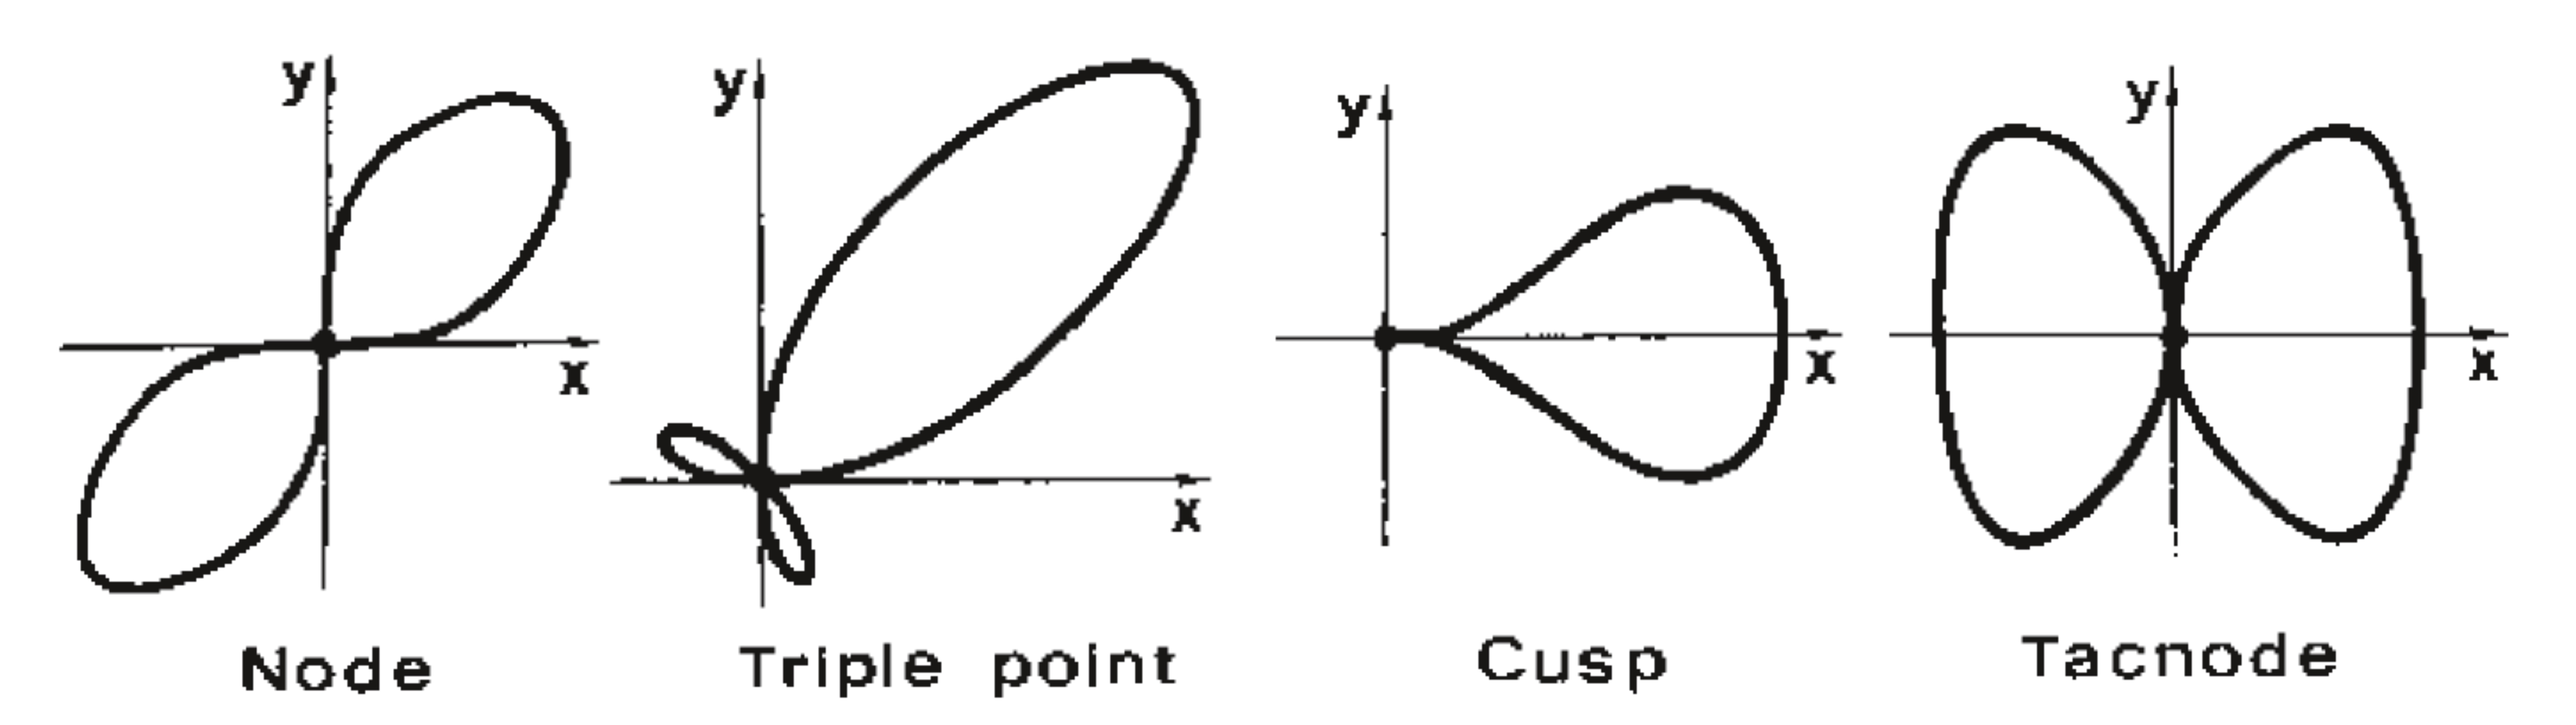
\includegraphics[width=0.8\columnwidth]{Figure4}\\
	Figure 4. 평면 곡선의 특이점
	\end{center}
	%
	\begin{enumerate}[label=,itemindent=0mm]
	\item Sol) Figure 4의 네 곡선은 차례대로 (b), (d), (c), (a)이다. 특이점은 모두 원점이다.\\
	\end{enumerate}
	%
	\begin{enumerate}[label=\tb{5.\arabic*.},itemindent=0mm,itemsep=4mm]
	\setcounter{enumi}{1}
	\item 다음과 같은 $\mb A^3$에서의 곡면들의 특이점의 위치를 찾고 특이점을 기술하라. ($\Char k\ne 2$라 가정하라.)
	각각의 방정식에 대응하는 곡선은 Figure 5에서 어떤 것인가?
	\begin{enumerate}[label=(\alph*)]
	\item $xy^2=z^2$
	\item $x^2+y^2=z^2$
	\item $xy+x^3+y^3=0$
	\end{enumerate}
	\end{enumerate}
	%
	%Figure 5
	\begin{center}
	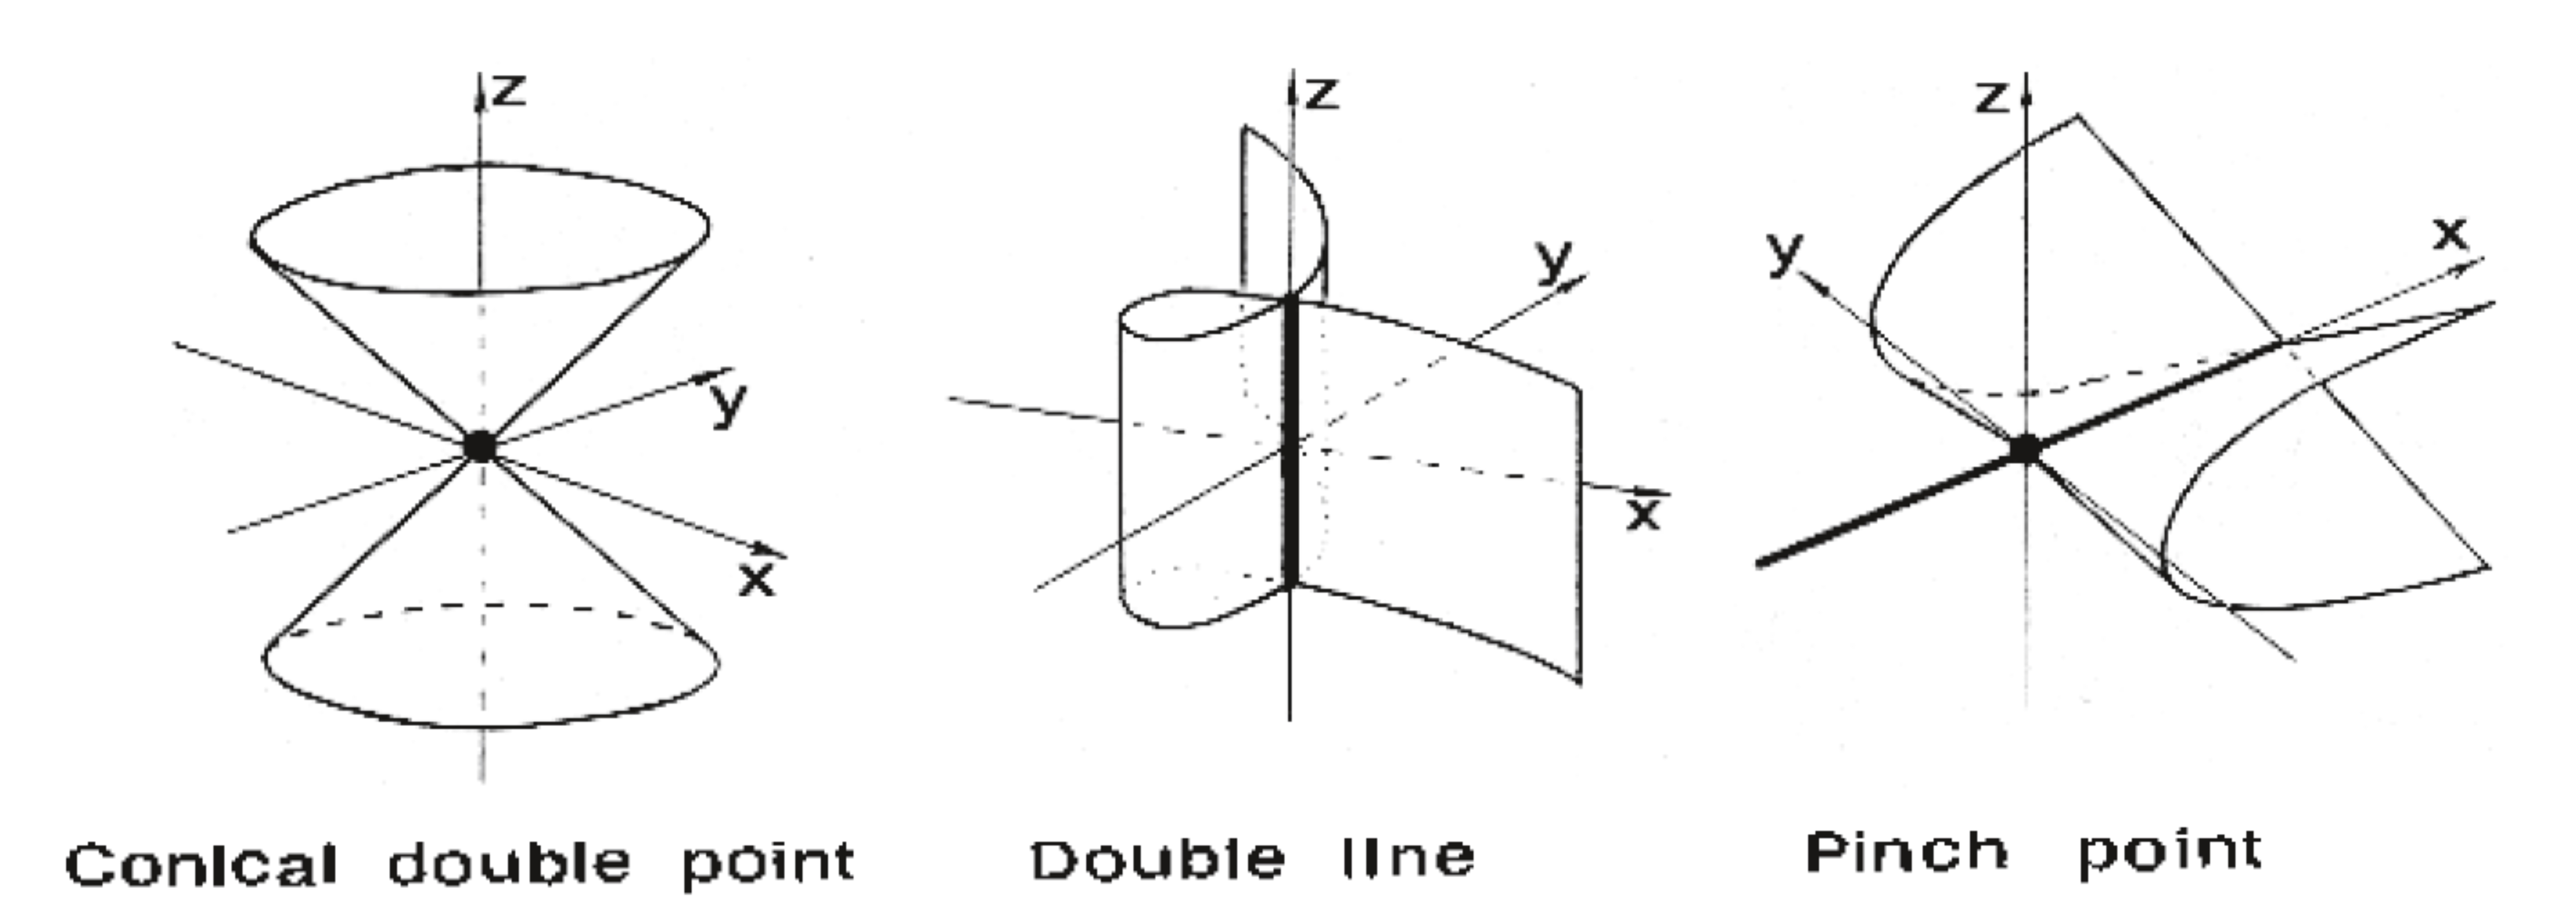
\includegraphics[width=0.8\columnwidth]{Figure5}\\
	Figure 5. 곡면 특이점
	\end{center}
	%
	\begin{enumerate}[label=,itemindent=0mm]
	\item Sol) Figure 5의 세 곡면은 순서대로 (b), (c), (a)이다. (a)의 특이점들은 $x$축, (b)의 특이점은 원점,
	(c)의 특이점들은 $z$축이다.\\
	\end{enumerate}
	%
	\begin{enumerate}[label=\tb{5.\arabic*.},itemindent=0mm,itemsep=4mm]
	\setcounter{enumi}{2}
	\item \tb{중복도.} $Y\bseq\mb A^2$가 방정식 $f(x,y)=0$에 의해 정의된 곡선이라 하자. $P=(a,b)$가 $\mb A^2$의 점이라 하자.
	좌표계를 1차다항식에 의해 변환하여 $P$가 점 $(0,0)$이 되도록 하자.
	그 후 $f$를 $x$와 $y$에 대한 $i$차 동차다항식 $f_i$들의 합 $f=f_0+f_1+\cdots+f_d$로 표현하자.
	$P$의 $Y$ 상에서의 \tb{중복도(multiplicity)}를 $f_r\ne 0$이도록 하는 최소 $r$로 정의하고 $\mu_P(T)$로 표기하자.
	($P\in Y\Lra\mu_P(Y)>0$임을 기억해 두라.) $f_r$의 선형 인수들은 $P$에서의 \tb{접선방향(tangent direction)}들이라 불린다.
	\begin{enumerate}[label=(\alph*)]
	\item $\mu_P(T)=1\Lra P$가 $Y$의 비특이점인 것임을 보여라.
	\item 위의 (Ex. 5.1)에 있는 각각의 특이점들의 중복도를 찾아라.
	\end{enumerate}
	%
	\sol (a) $f_1=\al x+\be y$라 하면 $\pa_xf(0,0)=\al,\pa_yf(0,0)=\be$이므로
	$f_r\ne 0$ iff $f$의 $(0,0)$에서의 Jacobian이 계수 1을 가짐 iff $P$가 비특이점인 것이다.\\
	(b) (Ex. 5.1)의 (a), (b), (c)의 특이점은 중복도 2이며 (d)의 특이점은 중복도 3이다.
	%
	\item \tb{교차 중복도.} 만약 $Y,Z\bseq\mb A^2$가 서로 다른 두 곡선이며 방정식 $f=0,g=0$에 의해 주어지고 만약 $P\in Y\cap Z$이면
		$Y$와 $Z$의 $P$에서의 \tb{교차 중복도(intersection multiplicity)} $(Y\cdot Z)_P$를
		$\mc O_P$-모듈 $\mc O_P/(f,g)$의 길이로 정의한다.
		\begin{enumerate}[label=(\alph*)]
			\item $(Y\cdot Z)_P$가 유한하며 $(Y\cdot Z)_P\ge\mu_P(Y)\cdot\nu_P(Z)$임을 보여라.
			\item 만약 $P\in Y$이면 $P$를 통과하는 거의 모든(i.e. 유한 개를 제외한 모든) 직선 $L$에 대하여 $(L\cdot Y)_P=\mu_P(Y)$임을 보여라.
			\item 만약 $Y$가 $\mb P^2$에서의 $d$차곡선이며 $L$이 $\mb P^2$에서의 직선이고 $L\ne Y$이면 $(L\cdot Y)=d$임을 보여라.
			여기에서 $(L\cdot Y)=\sum(L\cdot Y)_P$(모든 점 $P\in L\cap Y$에 대한 합)로 정의하며
			$(L\cdot Y)_P$는 $\mb P^2$의 적절한 아핀 덮개를 이용하여 정의된다.
		\end{enumerate}
	\item 모든 차수 $d>0$과 $p=0$ 또는 임의의 소수 $p$에 대하여 표수 $p$의 체 $k$ 상에서의
	$\mb P^2$에서의 비특이 $d$차곡선의 방정식을 제시하라.
	\item \tb{곡선 특이점의 부풀림.}
	\begin{enumerate}[label=(\alph*)]
	\item $Y$가 (Ex. 5.1)의 첨점 또는 결절점을 가지는 곡선이라 하자.
	$Y$를 $O=(0,0)$에서 부풀려 얻어진 곡선 $\tilde Y$는 비특이이다. (cf. (4.9.1)과 (Ex. 4.10))
	\item \tb{결절점(node)}(또는 \tb{통상2중점(ordinary double point)})을 서로 다른 접선방향(Ex. 5.3)들을 가지는
	평면 곡선의 2중점(i.e. 중복도 2의 점)으로 정의한다.
	만약 $P$가 평면 곡선 $Y$ 상에서의 결절점이면 $\ph^{-1}(P)$가 부풀려진 곡선 $\tilde Y$ 상에서의
	서로 다른 두 개의 비특이점들로 구성됨을 보여라. 우리는 `$P$를 부풀리는 것이 $P$에서의 특이점을 해소한다'고 말한다.
	\item $P\in Y$가 (Ex. 5.1)의 접촉절점이라 하자.
	만약 $\ph:\tilde Y\ra Y$가 $P$에서의 부풀림이면 $\ph^{-1}(P)$가 ($\Char k\ne 2$인 경우) 결절점임을 보여라.
	(b)를 이용하면 우리는 접촉절점이 2회의 순차적인 부풀림에 의해 해소될 수 있음을 알 수 있다.
	\item $Y$가 평면 곡선 $y^3=x^5$라 하자. 이는 $O$에서 `고차 첨점'을 가진다.
	$O$가 3중점임을 보여라; $O$를 부풀리는 것은 2중점을 제공한다. (어떠한 형태의 2중점인가?) 한 번 더 부풀리면 특이점이 해소된다.
	\end{enumerate}
	\ti{Note}: 우리는 나중에 (V, 3.8) 평면 곡선의 임의의 특이점이 유한 회의 순차적인 부풀림에 의해 해소될 수 있음을 보일 것이다.\\
	%
	\sol (a) (i) (Ex. 5.1)에서 첨점을 가지는 곡선은 $x^3-x^4=y^2+y^4$이다. 이를 원점에서 부풀리자.
	아핀 열린집합 $t=1$에서 $xu=y$와 $x=0$ 또는 $x^2(u^4+1)-x+u^2=0$을 얻는다.
	이곳에서 $E$와 $\tilde Y$의 교점은 $(x,y,u)=(0,0,0)$ 하나이다.
	$(0,0,0)$에서의 Jacobi 행렬 $\left(\begin{array}{ccc}0&1&0\\-1&0&0\end{array}\right)$가
	계수 $2=\codim Y$를 가지므로 $(0,0,0)$은 $\tilde Y$의 특이점이 아니다.
	아핀 열린집합 $u=1$에서 $x=ty$와 $y=0$ 또는 $y^2(1+t^4)-yt^3+1=0$을 얻는다.
	이곳에서는 $E$와 $\tilde Y$의 교점이 없다. 따라서 $\tilde Y$는 비특이이다.\\
	(ii) (Ex. 5.1)에서 결절점을 가지는 곡선은 $xy=x^6+y^6$이다. 이를 원점에서 부풀리자.
	아핀 열린집합 $t=1$에서 $xu=y$와 $x=0$ 또는 $x^4(1+u^6)-u=0$을 얻는다. Jacobi 행렬은 다음과 같다.
	%
	$$\left(\begin{array}{ccc}u&-1&x\\4x^3(1+u^6)&0&6x^4u^5-1\end{array}\right)$$
	%
	이는 $\tilde Y$의 모든 점에서 계수 2를 가진다. $u=1$에서도 동일하게 계산하면 $\tilde Y$가 비특이임이 따라온다.\\
	(b) (1차다항식에 의한 적절한 좌표변환을 거친 후) $Y$를 정의하는 다항식 $f$는 $xy+f_{3+}(x,y)$이다.
	($f_{3+}\sum_{n\ge 3}f_n$은 3차 이상의 항만 가지는 다항식이다.) 원점에서 이를 부풀리자.
	$g(x,u)=x^{-2}f_{3+}(x,xu)$라 하자. (이러한 $g$는 $x$에 대하여 1차 이상의 항만 가지는 다항식이다.)
	아핀 열린집합 $t=1$에서 $xu=y$와 $x=0$ 또는 $u+g(x,u)=0$을 얻는다.
	따라서 $t=1$ 내에서 $E$와 $\tilde Y$의 교점은 $(x,y,t,u)=(0,0,1,0)$ 하나이다.
	Jacobian은 $\left(\begin{array}{ccc}0&-1&0\\a&0&1\end{array}\right)$로 계수 2를 가진다. 따라서 $(0,0,1,0)$은 비특이점이다.
	마찬가지로 $u=1$에서 교점은 비특이점 $(0,0,0,1)$ 하나이다. 즉 $\ph^{-1}(P)$는 서로 다른 두 비특이점들로 구성된다.\\
	(c) (Ex. 5.1)에서 접촉절점을 가지는 곡선은 $x^2=x^4+y^4$이다. 이를 원점에서 부풀리자.
	아핀 열린집합 $t=1$에서 $xu=y$와 $x=0$ 또는 $1=x^2(1+u^2)$를 얻는다.
	따라서 $t=1$에서 $E$와 $\tilde Y$는 교차하지 않는다.
	아핀 열린집합 $u=1$에서 $x=ty$와 $y=0$ 또는 $t^2=y^2(t^4+1)$를 얻는다.
	따라서 $u=1$에서 $E$와 $\tilde Y$는 한 점 $(x,y,t)=(0,0,0)$에서 교차한다.
	$\tilde Y$를 평면 $x=ty$에서의 곡선으로 간주하면 위 교점에서 $f_2=y^2-t^2=(y-t)(y+t)$이므로 $\Char k\ne 2$인 경우 결절점이다.
	($\Char k=2$인 경우 $y+t=yt^2$이므로 비특이점이다.) (b)에 의해 이는 추가적인 부풀림에 의해 해소될 수 있다.\\
	(d) $f_1=f_2=0,f_3=y^3\ne 0$이므로 $Y$는 $O$에서 3중점을 가진다. 이를 $O$에서 부풀리자.
	아핀 열린집합 $u=1$에서 $x=ty$와 $y=0$ 또는 $1=t^5y^2$를 얻는다. 따라서 $u=1$에서 $E$와 $\tilde Y$는 교차하지 않는다.
	아핀 열린집합 $t=1$에서 $xu=y$와 $x=0$ 또는 $u^3=x^2$를 얻는다.
	따라서 $t=1$에서 $E$와 $\tilde Y$는 한 점 $(x,y,u)=(0,0,0)$에서 교차한다.
	$\tilde Y$를 평면 $xu=y$에서의 곡선으로 간주하면 $(x,u)=(0,0)$은 첨점이다.
	(a) (i)과 마찬가지 방식으로 부풀림을 통해 첨점을 해소할 수 있다.
	%
	\item $Y\bseq\mb P^2$가 방정식 $f(x,y,z)=0$에 의해 정의된 1차 초과의 비특이 평면 곡선이라 하자.
	$X\bseq\mb A^3$이 $f$에 의해 정의된 아핀 대수다양체라 하자. (이는 $Y$ 상에서의 뿔이다; (Ex. 2.10)을 참조하라.)
	$P$가 뿔의 \tb{꼭짓점(vertex)}인 점 $(0,0,0)$이라 하자. $\ph:\tilde X\ra X$가 $X$의 $P$에서의 부풀림이라 하자.
	\begin{enumerate}[label=(\alph*)]
	\item $X$가 하나의 특이점 $P$만을 가짐을 보여라.
	\item $\tilde X$가 비특이임을 보여라. (이를 아핀 열린집합들로 덮어라.)
	\item $\ph^{-1}(P)$가 $Y$와 동형임을 보여라.
	\end{enumerate}
	\item $Y\bseq\mb P^n$이 $r$차원 사영 대수다양체라 하자.
	$f_1,\ldots,f_t\in S=k[x_0,\ldots,x_n]$이 $Y$의 아이디얼을 생성하는 동차다항식들이라 하자.
	$P\in Y$가 동차 좌표 $P=(a_0,\ldots,a_n)$을 가지는 점이라 하자.
	$P$가 $Y$ 상에서 비특이일 필요충분조건은 행렬 $\|(\pa f_i/\pa x_j)(a_0,\ldots,a_n)\|$의 계수가 $n-r$인 것임을 보여라.
	[Hint: (a) 이러한 계수가 $P$에 대하여 선택된 동차 좌표에 독립적임을 보여라.
	(b) $P$를 포함하는 아핀 열린집합 $U_i\bseq\Pn$으로 보내고 아핀 Jacobi 행렬을 사용하라.
	(c) $f$가 $d$차 동차이면 $\sum x_i(\pa f/\pa x_i)=d\cdot f$라는 Euler 보조정리가 필요할 것이다.]\\
	%
	\sol $f_i$의 차수를 $d_i$로 표기하면 동차 좌표의 $a$배는 Jacobi 행렬의 $i$행이 $a^{d_i-1}$배가 되는 효과를 준다.
	이는 행렬의 계수에 영향을 주지 않는다.
	일반성을 잃지 않고 $P\in U_0$라 하자. 좌표를 $x_0=1$이도록 선택하자.
	그 경우 $P$에서의 아핀 Jacobi 행렬 $J_A$는 사영 Jacobi 행렬 $J_P$ 1열($x_0$에 대한 편도함수들)이 제거된 것이다.
	Euler 보조정리에 의해 $\sum x_i(P)(\pa f/\pa x_i)(P)=d\cdot f(P)=0$이므로
	1열은 어떠한 경우에도 다른 열들의 선형 결합으로 표현 가능하다; 따라서 1열의 제거는 계수에 영향을 주지 않는다.
	국소환과 그 극대 아이디얼 $\mf m$은 열린 근방에만 영향을 받으므로 아핀 경우와 사영 경우에 동일하다.
	$\rank J_P=\rank J_A=n-\dim\mf m/\mf m^2$이므로 $P$가 비특이 iff $\dim\mf m/\mf m^2=r$ iff $\rank J_P=n-r$이다.
	%
	\item $f\in k[x,y,z]$가 동차다항식이고 $Y=Z(f)\bseq\mb P^2$가 $f$에 의해 정의된 대수적 집합이며
	모든 $P\in Y$에 대하여 $(\pa f/\pa x)(P),(\pa f/\pa y)(P),(\pa f/\pa z)(P)$ 중 적어도 하나가 0이라 하자.
	$f$가 기약(이며 따라서 $Y$가 비특이 대수다양체)임을 보여라. [Hint: (Ex 3.7)을 사용하라.]
	\item 대수다양체 $X$ 상에서의 점 $P$에 대하여 $\mf m$이 국소환 $\mc O_P$의 극대 아이디얼이라 하자.
	$X$의 $P$에서의 \tb{Zariski 접공간(Zariski tangent space)} $T_P(X)$를 $\mf m/\mf m^2$의 쌍대 $k$-벡터 공간으로 정의한다.
	\begin{enumerate}[label=(\alph*)]
	\item 임의의 점 $P\in X$에 대하여 $\dim T_P(X)\ge\dim X$이며 등호가 성립할 필요충분조건은 $P$가 비특이점인 것이다.
	\item 임의의 사상 $\ph:X\ra Y$에 대하여 자연스러운 유도 $k$-선형 사상 $T_P(\ph):T_P(X)\ra T_{\ph(P)}(Y)$가 존재한다.
	\item 만약 $\ph$가 포물선 $x=y^2$의 $x$축 상으로의 종방향 사영이면 원점에서의 접공간의 유도 사상 $T_0(\ph)$가 0 사상임을 보여라.
	\end{enumerate}
	\item \tb{$\mb P^3$에서의 타원 4차곡선.} $Y$가 방정식 $x^2-xz-yw=0$과 $yz-xw-zw=0$에 의해 정의된
	$\mb P^3$에서의 대수적 집합이라 하자. $P$가 점 $(x,y,z,w)=(0,0,0,1)$이며 $\ph$가 $P$에서 평면 $w=0$으로의 사영이라 하자.
	$\ph$가 $Y-P$와 평면 3차곡선 $y^2z-x^3+xz^2=0$에서 점 $(1,0,-1)$을 제외한 것 간의 동형사상을 유도함을 보여라.
	그 후 $Y$가 기약 비특이 곡선임을 보여라. 이는 $\mb P^3$에서의 \tb{타원 4차곡선(eliptic quartic curve)}이라 불린다.
	이것이 두 방정식에 의해 정의되었으므로 이는 완비 교집합의 또 다른 예시이다. (Ex. 2.17)\\
	%
	\sol $Y$를 정의하는 두 식에서 $w$를 소거하여 $x(x^2-z^2)=(x+z)yw=y^2z$를 얻는다.
	즉 $\ph(Y-P)$는 $y^2z-x^3+xz^2=0$의 부분집합이다.
	$w$는 $y\ne 0$인 경우에는 $(x-z)x/y$이고 $x+z\ne 0$인 경우에는 $yz/(x+z)$으로 복원될 수 있다;
	$y\ne 0,x+z\ne 0$이며 $y^2z-x^3+xz^2=0$이 성립한다면 이러한 두 가지 $w$가 동일하므로 역이 모순 없이 잘 정의된다.
	그러나 $y=x+z=0$인 경우, 즉 $(1,0,-1)$은 $\ph(Y-P)$에 속하지 않는다.
	($Z(y^2z-x^3+xz^2)=Y'$이라 표기하면) 이는 $\ph$가 $Y-P$와 $Y'-\{(1,0,-1)\}$ 간의 동형사상임을 보여준다.
	도함수 $(z^2,0,y^2)$가 0이 되지 않으므로 $Y'$은 비특이이다. 따라서 $Y$도 $P$ 이외의 가능한 특이점이 없다.
	$Y$의 $P$에서의 Jacobian은 다음과 같다:
	%
	$$\left(\begin{array}{cccc}2x-z&-w&-x&-y\\-w&z&y-w&-x-z\end{array}\right)(0,0,0,1)
	=\left(\begin{array}{cccc}0&-1&0&0\\-1&0&-1&0\end{array}\right)$$
	%
	이는 계수 2를 가진다. 따라서 $Y$는 비특이이다.\\
	$y^2z-x^3+xz^2=fg,\deg f\ne 0,\deg g\ne 0$이라 가정하면 Theorem 7.2에 의해 $f$와 $g$의 공통영점이 존재하며
	이 점에서 $\pa_{x_i}(fg)=(\pa_{x_i}f)g+f(\pa_{x_i}g)=0$이므로 비특이성에 모순이다. 따라서 $Y'$은 기약이다.
	기약 대수적 집합의 열린 부분집합은 조밀하므로 임의의 두 열린 부분집합이 교차하며 따라서 $Y'-\{(1,0,1)\}$은 연결이다.
	그러므로 이와 동형인 $Y$에서의 열린집합 $Y-P$도 연결이다. $Y$가 공집합이 아닌 서로 소 열린집합 $Y_1,Y_2$로 분할된다면
	(한 점 집합 $P$가 공집합이 아닌 열린집합을 포함하지 못하므로) $Y_1,Y_2$는 모두 $Y-P$와 교차하며 따라서 $Y-P$의 연결성에 모순이다.
	따라서 $Y$는 연결이다.\\
	임의의 연결 비특이 대수적 집합은 기약이며 따라서 비특이 대수다양체이다: 먼저 좌표환의 정의를 임의의 대수적 집합으로 확대하자.
	기약 성분이 2개 이상 존재한다 하자. 연결성에 의해 임의의 두 기약 성분은 교차한다. $x$가 2개 이상의 기약 성분의 교집합에 속한다 하자.
	비특이성에 의해 $\mc O_x$가 정칙 국소환이다. 정칙 국소환은 정역이다. (가환대수학 교재를 참조하라.)
	따라서 $\mc O_x$는 $(0)$을 유일한 극소 소 아이디얼로 가진다.
	$\mc O_x$의 극소 소 아이디얼들은 $x$를 포함하는 기약 성분들에 대응된다.
	이는 $x$가 2개 이상의 기약 성분에 속함에 모순이다. 따라서 주장이 증명된다.
	%
	\item \tb{2차초곡면.} $\Char k\ne 2$이며 $f$가 $x_0,\ldots,x_n$에 대한 2차 동차다항식이라 하자.
	\begin{enumerate}[label=(\alph*)]
	\item 좌표계를 적절한 1차다항식에 의해 변환하는 것으로 어떠한 $0\le r\le n$에 대하여
	$f$가 $f=x_0^2+\cdots+x_r^2=0$의 형태가 될 수 있음을 보여라.
	\item $f$가 기약일 필요충분조건은 $r\ge 2$인 것임을 보여라.
	\item $r\ge 2$라 가정하고 $Q$가 $f$에 의해 정의된 $\Pn$에서의 2차초곡면이라 하자.
	$Q$의 특이 자취 $Z=\Sing Q$가 $n-r-1$차원 \ti{선형} 대수다양체(Ex. 2.11)임을 보여라.
	특히 $Q$가 비특이일 필요충분조건은 $r=n$인 것이다.
	\item $r<n$인 경우 $Q$는 축이 $Z$인 비특이 2차초곡면 $Q'\bseq\mb P^r$ 상에서의 뿔임을 보여라.
	(이러한 뿔의 개념은 (Ex. 2.10)에서 정의된 것의 일반화이다. 만약 $Y$가 $\mb P^r$의 닫힌 부분집합이며
	$Z$가 $\Pn$에서의 $n-r-1$차원 선형 부분공간이면 $\mb P^r$을 $\Pn$에 매장하여 $\mb P^r\cap Z=\es$이도록 하고
	\tb{축이 $Z$인 $Y$ 상에서의 뿔(cone over $Y$ with axis $Z$)}를 $Y$의 점과 $Z$의 점을 통과하는 모든 직선들의 합집합으로 정의한다.)
	\end{enumerate}
	\item 모든 정칙 국소환은 정수적으로 닫힌 정역이다. (Matsumura [2, Th. 36, p. 121])
	그러므로 (5.3)에 의해 임의의 대수다양체는 정규점들의 공집합이 아닌 열린 부분집합을 가짐을 알 수 있다. (Ex. 3.17)
	이 연습문제에서 ((5.3)을 사용하지 않고) 대수다양체의 비정규점들의 집합이 닫힌 진부분집합임을 보여라.
	(정수적 폐포의 유한성이 필요할 것이다: (3.9A)를 참조하라.)
	\item \tb{해석적 동형 특이점.}
	\begin{enumerate}[label=(\alph*)]
	\item 만약 $P\in Y$와 $Q\in Z$가 해석적 동형 평면 곡선 특이점이면 중복도 $\mu_P(Y)$와 $\mu_Q(Z)$가 동일함을 보여라. (Ex. 5.3)
	\item 본문의 예시 (5.6.3)을 일반화하여 만약 $f=f_r+f_{r+1}+\cdots\in k[[x,y]]$이며
	$f$의 최고차 형식 $f_r$이 $f_r=g_sh_t$로 분해되고 $g_s,h_t$가 각각 $s$차와 $t$차 동차이며
	공통 1차 인수를 갖지 않으면 $k[[x,y]]$에서의 형식적 멱급수
	%
	\begin{align*}
	g&=g_s+g_{s+1}+\cdots\\h&=h_t+h_{t+1}+\cdots
	\end{align*}
	%
	가 존재하여 $f=gh$를 만족시킨다.
	\item $Y$가 $\mb A^2$에서 방정식 $f(x,y)=0$에 의해 정의되며 $P=(0,0)$이 $Y$ 상에서의 중복도 $r$인 점이고
	따라서 $f$가 $x$와 $y$에 대한 다항식으로 전개되었을 경우 $f=f_r+$고차항 형태이다.
	$P$가 \tb{통상$r$중점(ordinary $r$-fold point)}임을 $f_r$이 서로 다른 $r$개 선형 인수들의 곱인 것으로 정의한다.
	임의의 두 통상2중점이 해석적 동형임을 보여라. 통상3중점에 대해서도 위와 같다.
	그러나 서로 동형이 아닌 통상4중점들의 1매개변수족이 존재함을 보여라.
	\end{enumerate}
		\begin{enumerate}[label=*(\alph*)]
			\setcounter{enumii}{3}
			\item $\Char k\ne 2$라 가정하자. 평면곡선의 임의의 2중점들이 유일하게 결정된 $r\ge 2$에 대하여
			곡선 $y^2=x^r$의 $(0,0)$에서의 특이점과 해석적 동형임을 보여라.
			만약 $r=2$이면 이는 결절점이다. (Ex. 5.6) 만약 $r=3$이면 이는 \tb{첨점(cusp)}이다;
			만약 $r=4$이면 \tb{접촉절점(tacnode)}이다. 심화된 논의를 위해서는 (V, 3.9.5)를 참조하라.
		\end{enumerate}
		\item \tb{평면 곡선들의 족.} 3변수 $x,y,z$에 대한 $d$차 동차다항식 $f$는 $\binom{d+2}2$개 계수들을 가진다.
		이러한 계수들이 $N=\binom{d+2}2-1=\fra 2d(d+3)$인 $\mb P^N$에서의 점을 표현한다 하자.
		\begin{enumerate}[label=(\alph*)]
			\item 이것이 $\mb P^N$의 점들과 $d$차방정식에 의해 정의될 수 있는 $\mb P^2$의 대수적 집합들 간의 대응 관계를 제공함을 보여라.
			$f$가 다수의 인자를 가지는 몇 가지 경우를 제외하면 이러한 대응이 일대일임을 보여라.
			\item 이러한 대응 하에서 (기약) 비특이 $d$차곡선들이 $\mb P^N$의 공집합이 아닌 Zariski-열린 부분집합의 점들에
			일대일 대응됨을 보여라. [Hint: (1) 동차다항식 $\pa f/\pa x_0,\ldots,\pa f/\pa x_n$에 적용된 소멸 이론 (5.7A)를 사용하라.
			(2) 위의 (Ex. 5.5, 5.8, 5.9)를 사용하라.]
		\end{enumerate}
	\end{enumerate}
	
	
	
	\subsection*{Section I.6}
	
	\begin{enumerate}[label=\tb{6.\arabic*.},itemindent=0mm,itemsep=4mm]
		\item \tb{유리(rational)} 곡선이 $\mb P^1$과 쌍유리동치인 곡선임을 상기하라. (Ex. 4.4)
		$Y$가 $\mb P^1$과 동형이 아닌 비특이 유리곡선이라 하자.
		\begin{enumerate}[label=(\alph*)]
			\item $Y$가 $\mb A^1$의 열린 부분집합과 동형임을 보여라.
			\item $Y$가 아핀임을 보여라.
			\item $A(Y)$가 유일 인수분해 정역임을 보여라.
		\end{enumerate}
		\item \tb{타원곡선.} $Y$가 $\mb A^2$에서의 곡선 $y^2=x^3-x$라 하고 기반체 $k$의 표수가 2가 아니라 하자.
		이 연습문제에서 우리는 $Y$가 유리 곡선이 아니며 따라서 $K(Y)$가 $k$의 순수히 초월적 확대가 아님을 보일 것이다.
		\begin{enumerate}[label=(\alph*)]
			\item $Y$가 비특이임을 보이고 $A=A(Y)\cong k[x,y]/(y^2-x^3+x)$가 정수적으로 닫힌 정역임을 연역하라.
			\item $k[x]$가 $x$의 $A$에서의 상에 의해 생성된 $K=K(Y)$의 부분환이라 하자.
			$k[x]$가 다항식환이며 $A$가 $k[x]$의 $K$에서의 정수적 폐포임을 보여라.
			\item 자기동형사상 $\si:A\ra A$가 존재하여 $y$를 $-y$로 대응시키며 $x$를 고정함을 보여라.
			임의의 $a\in A$에 대하여 $a$의 \tb{노름(norm)}을 $N(a)=a\cdot\si(a)$로 정의하자.
			$N(a)\in k[x],N(1)=1$이며 임의의 $a,b\in A$에 대하여 $N(ab)=N(a)\cdot N(b)$임을 보여라.
			\item 노름을 사용하여 $A$에서의 가역원들이 정확히 $k$의 0이 아닌 원소들임을 보여라.
			$x$와 $y$가 $A$의 기약원임을 보여라. $A$가 유일 인수분해 정역이 \ti{아님}을 보여라.
			\item $Y$가 유리 곡선이 아님을 보여라. (Ex. 6.1)
			이러한 중요한 결과의 다른 증명을 위해서는 (II, 8.20.3)과 (III, Ex. 5.3)을 참조하라.
		\end{enumerate}
		\item (a) $\dim X\ge 2$ 또는 (b) $Y$가 사영 대수다양체가 아니면 (6.8)의 결과가 거짓임을 반례를 통해 보여라.
		\item $Y$가 비특이 사영 곡선이라 하자. 상수함수가 아닌 $Y$ 상에서의 모든 유리함수가 전사 사상 $\ph:Y\ra\mb P^1$을 정의하며
		모든 $P\in\mb P^1$에 대하여 $\ph^{-1}(P)$가 유한집합임을 보여라.
		\item $X$가 비특이 사영 곡선이라 하자. $X$가 대수다양체 $Y$의 (국소 닫힌) 부분다양체라 하자. (Ex. 3.10)
		$X$가 사실 $Y$의 닫힌 부분집합임을 보여라. 일반화를 위해서는 (II, Ex. 4.4)를 참조하라.
		\item \tb{$\mb P^1$의 자기동형사상.} $\mb P^1$을 $\mb A^1\cup\{\infty\}$로 간주하자.
		그 경우 $\mb P^1$의 \tb{선형 분수 변환(fractional linear transformation)}을
		$a,b,c,d\in k,ad-bc\ne 0$에 대하여 $x\mt(ax+b)/(cx+d)$로 대응시키는 것으로 정의하자.
		\begin{enumerate}[label=(\alph*)]
			\item 선형 분수 변환이 $\mb P^1$의 \tb{자기동형사상(automorphism)}(i.e. $\mb P^1$과 자기 자신의 동형사상)을 유도함을 보여라.
			이러한 모든 선형 분수 변환들의 군을 $\mrm{PGL}(1)$로 표기할 것이다.
			\item $\Aut\mb P^1$이 $\mb P^1$의 모든 자기동형사상들의 군을 나타낸다 하자.
			$\Aut\mb P^1\simeq\Aut k(x)$(체 $k(x)$의 $k$-자기동형사상들의 군)임을 보여라.
			\item 이제 $k(x)$의 모든 자기동형사상이 선형 분수 변환임을 보이고 $\mrm{PGL}(1)\ra\Aut\mb P^1$이 동형사상임을 연역하라.
		\end{enumerate}
		\ti{Note}: 우리는 나중에(II, 7.1.1) 유사한 결과가 $\Pn$에 대하여 성립함을 보일 것이다:
		모든 자기동형사상은 도앛 좌표들의 선형 변환에 의해 주어진다.
		\item $P_1,\ldots,P_r,Q_1,\ldots,Q_s$가 $\mb A^1$의 서로 다른 점들이라 하자.
		만약 $\mb A^1-\{P_1,\ldots,P_r\}$이 $\mb A^1-\{Q_1,\ldots,Q_s\}$와 동형이면 $r=s$임을 보여라. 역이 참인가? cf. (Ex. 3.1)
	\end{enumerate}
	
	
	
	\subsection*{Section I.7}
	
	\begin{enumerate}[label=\tb{7.\arabic*.},itemindent=0mm,itemsep=4mm]
	\item \begin{enumerate}[label=(\alph*)]
	\item $\Pn$의 $\mb P^N$으로의 $d$차 매장(Ex. 2.12)의 차수를 찾아라. [답: $d^n$]
	\item $\mb P^r\times\mb P^s$의 $\mb P^N$으로의 Segre 매장(Ex. 2.14)의 차수를 찾아라. [답: $\binom{r+s}r$]
	\end{enumerate}
	%
	\sol (a) (Ex. 2.12)에 의해 동차 좌표환은 등급 대수로서 $d$차 단항식들에 의해 생성된 $k[x_0,\ldots,x_n]$의 부분대수와 동형이다.
	그러므로 $l$급 원소들은 $x_i$들에 대한 $dl$차 동차다항식들이며 따라서 $\ph_Y(l)={}_{n+1}H_{dl}=\binom{n+dl}{n}$이다.
	그러므로 $P_Y(z)=\binom{n+dz}n$이며 따라서 차수는 $n!\cdot\frac{d^n}{n!}=d^n$이다.\\
	(b) (Ex. 2.14)에 의해 동차 좌표환은 등급 대수로서 $x_iy_k$들에 의해 생성된
	$k[x_0,\ldots,x_r,y_0,\ldots,y_s]$의 부분대수와 동형이다.
	그러므로 $l$급 원소들은 $x_i$에 대하여 $l$차 동차, $y_i$에 대하여 $l$차 동차인 다항식들이며
	따라서 $\ph_Y(l)=\binom{r+l}l\binom{r+l}l=\binom{r+l}{r}\binom{s+l}s$이다.
	그러므로 $P_Y(z)=\binom{r+z}r\binom{s+z}s$이며 따라서 차수는 $(r+s)!\cdot\fra{r!s!}=\binom{r+s}r$이다.
	%
	\item $Y$가 $\Pn$에서의 $r$차원 대수다양체이며 Hilbert 다항식 $P_Y$를 가진다 하자.
	$Y$의 \tb{산술종수(arithmetic genus)}를 $p_a(Y)=(-1)^r(P_Y(0)-1)$로 정의하자.
	이는 $Y$의 사영 매장에 독립적인 중요한 불변량이다. (나중에 이를 (III, Ex. 5.3)에서 보게 될 것이다.)
	\begin{enumerate}[label=(\alph*)]
	\item $p_a(\Pn)=0$임을 보여라.
	\item 만약 $Y$가 평면 $d$차곡선이면 $p_a(Y)=\fra 2(d-1)(d-2)$임을 보여라.
	\item 더 일반적으로 만약 $H$가 $\Pn$에서의 $d$차 초곡면이면 $p_a(H)=\binom{d-1}n$이다.
	\item 만약 $Y$가 $\mb P^3$에서의 차수 $a,b$인 곡면들의 완비 교집합이면 (Ex. 2.17)
	$p_a(Y)=\fra 2ab(a+b-4)+1$이다.
	\item $Y^r\bseq\Pn,Z^s\bseq\mb P^m$이 사영 대수다양체라 하고
	$Y\times Z\bseq\Pn\times\mb P^m\ra\mb P^N$으로 Segre 매장에 의해 매장하자. 다음이 성립함을 보여라.
	%
	$$p_a(Y\times Z)=p_a(Y)p_a(Z)+(-1)^sp_a(Y)+(-1)^rp_a(Z)$$
	%
	\end{enumerate}
	%
	\sol (a) $\Pn$에 대하여 $\ph_{\Pn}(l)=\binom{n+l}n,P_{\Pn}(z)=\binom{n+z}n$, 차수 $n!\fra{n!}=1$이므로
	산술종수 $p_a(\Pn)=(-1)^n(1-1)=0$이다.\\
	(b) 평면 $d$차곡선은 단일한 $d$차 동차다항식 $f$에 의해 생성되며
	이러한 $f$는 동차 좌표환 내에서 $d$차 동차다항식들 간의 선형 종속 관계가 된다.
	따라서 $\ph_Y(l)$은 $l\le d$이면 $\binom{l+2}2$,
	$l\ge d$이면 $\binom{l+2}2-\binom{l-d+2}2$이다. ($f$를 인자로 가지는 다항식들 제외)
	그 경우 $P_Y(z)=\binom{z+2}2-\binom{z-d+2}2=\fra 2(z+2)(z+1)-\fra 2(z-d+2)(z-d+1)=zd-\frac{d^2-3d}2$이다.
	따라서 $P_Y(0)=-(d^2-3d)/2$이며 $p_a(Y)=(-1)(P_Y(0)-1)=(d-1)(d-2)/2$이다.\\
	(c) $d$차초곡면도 마찬가지로 단일한 $d$차 동차다항식에 의해 생성되므로 $\ph_Y(l)$은 $l\le d$이면 $\binom{l+n}n$,
	$l\ge d$이면 $\binom{l+n}n-\binom{l-d+n}n$이며 따라서 $P_Y(z)=\binom{z+n}n-\binom{z-d+n}n$이고
	$P_Y(0)=1+(-1)^{n+1}(d-n)\cdots(d-1)/n!$이다. 그러므로 $p_a(Y)=(-1)^{n-1}(P_Y(0)-1)=(d-1)\cdots(d-n)/n!=\binom{d-1}n$이다.\\
	(d) $Y=X_1\cap X_2,X_i=Z(f_i),\deg f_1=a,\deg f_2=b$라 하자. $X_1\cup X_2=Z(f_1f_2)$이므로 $\deg X_1\cup X_2=a+b$이다.
	다음의 완전열에 의해,
	%
	$$0\ra S/(f_1f_2)\ra S/(f_1)\oplus S/(f_2)\ra S/(f_1,f_2)\ra 0$$
	%
	$P_Y=P_{X_1}+P_{X_2}-P_{X_1\cup X_2}=\binom{z+3}3-\binom{z-a+3}3-\binom{z-b+3}3+\binom{z-a-b+3}3$이다.
	그러므로 $p_a(Y)=(-1)^1[\binom{3-a-b}3-\binom{3-a}3-\binom{3-b}3]=\fra 2ab(a+b-4)+1$이다.\\
	(e) $Y$와 $Z$의 동차 좌표환을 각각 $\bigoplus_iM_i\bseq k[x_0,\ldots,x_n]$과
	$\bigoplus N_i\bseq k[y_0,\ldots,y_m]$으로 분해하면
	$X\times Y$의 동차 좌표환은 $\bigoplus_iM_i\otimes N_i$와 동형이다. cf. (Ex. 2.14), (Ex. 7.1b).
	텐서곱의 차원은 곱인자의 차원의 곱이므로 $\ph_{Y\times Z}(l)=\ph_Y(l)\ph_Z(l)$이며 따라서 $\ph_{Y\times Z}=\ph_Y\ph_Z$이다.
	그러므로 $P_{Y\times Z}=P_YP_Z$이며 $p_a(Y\times Z)=(-1)^{r+s}(P_Y(0)P_Z(0)-1)
	=(-1)^{r+s}[(P_Y(0)-1)(P_Z(0)-1)+(P_Y(0)-1)+(P_Z(0)-1)]=p_a(Y)p_a(Z)+(-1)^sp_a(Y)+(-1)^rp_a(Z)$이다.
	%
		\item \tb{쌍대 곡선.} $Y\bseq\mb P^2$가 곡선이라 하자.
		직선 $L:a_0x_0+a_1x_1+a_2x_2=0$의 동차 좌표를 $(a_0,a_1,a_2)$로 취하여
		$\mb P^2$에 속한 직선들의 집합을 다른 사영공간 $(\mb P^2)^*$로 간주하자.
		각각의 비특이점 $P\in Y$에 대하여 유일한 직선 $T_P(Y)$가 존재하여 $Y$와의 $P$에서의 교차 중복도가 1 초과이도록 한다.
		이는 $Y$의 $P$에서의 \tb{접선(tangent line)}이다.
		함수 $P\mt T_P(Y)$가 $\mrm{Reg}\:Y$($Y$의 비특이점들의 집합)에서 $(\mb P^2)^*$로의 \ti{사상}을 정의함을 보여라.
		이 사상의 상의 폐포는 $Y$의 쌍대 곡선 $Y^*\bseq(\mb P^2)^*$라 불린다.
		\item $\mb P^2$에서의 $d$차 곡선 $Y$가 주어진 경우 $(\mb P^2)^*$의 Zariski 위상 하에서의 공집합이 아닌 열린 부분집합
		$U$가 존재하여 각각의 $L\in U$에 대하여 $L$이 $Y$와 정확히 $d$개 점에서 교차하도록 할 수 있다.
		[Hint: $Y$에 접하거나 또는 $Y$의 특이점을 지나는 $(\mb P^2)^*$에서의 직선들의 집합이 진부분집합에 포함됨을 보여라.]
		이 결과는 $Y$의 차수를 $\mb P^2$에서의 거의 모든 직선이 $Y$와 $d$개 점에서 만나도록 하는 수 $d$로 정의할 수 있었음을 보여준다.
		(여기에서 `거의 모든'은 쌍대 사영공간 $(\mb P^2)^*$와 동일시된 직선들의 집합의 공집합이 아닌 열린집합을 의미한다.)
		\item \begin{enumerate}[label=(\alph*)]
			\item $\mb P^2$에서의 $d>1$차 기약 곡선 $Y$는 중복도 $d$ 이상의 점을 가질 수 없음을 보여라. (Ex. 5.3)
			\item 만약 $Y$가 $d>1$차 기약 곡선이며 중복도 $d-1$인 점을 가지면 $Y$는 유리 곡선이다. (Ex. 6.1)
		\end{enumerate}
		\item \tb{선형 대수다양체.} 순수히 $r$차원인(i.e. 모든 기약 성분이 $r$차원인) 대수적 집합 $Y$가 차수 1을 가질 필요충분조건은
		$Y$가 선형 대수다양체(Ex. 2.11)인 것임을 보여라. [Hint: 먼저 (7.7)을 사용하여 $\dim Y=1$인 경우를 다루어라.
		그 후 초평면으로 자르고 귀납법을 사용하여 일반적인 경우를 다루어라.]
		\item $Y$가 $\Pn$에서의 차원 $r$이며 차수 $d>1$의 대수다양체라 하자. $P\in Y$가 비특이점이라 하자.
		$Q\in Y,Q\ne P$에 대하여 $X$를 모든 직선 $PQ$들의 합집합의 폐포로 정의하자.
		\begin{enumerate}[label=(\alph*)]
			\item $X$가 $r+1$차원 대수다양체임을 보여라.
			\item $\deg X<d$임을 보여라. [Hint: $\dim Y$에 대한 귀납법을 사용하라.]
		\end{enumerate}
		\item $Y^r\bseq\Pn$이 2차 대수다양체라 하자. $Y$가 $\Pn$에서의 $r+1$차원 선형 부분공간 $L$에 포함됨을 보여라.
		그러므로 $Y$는 $\mb P^{r+1}$에서의 2차초곡면과 동형이다. (Ex. 5.12)
	\end{enumerate}
	
	
	
	\section*{Chapter II}
	
	\subsection*{Section II.1}
	
	\begin{lemma*}
	%
		\tn{\\$\phi,\psi:\ms F\ra\ms G$가 위상공간 $X$ 상에서의 층 사상이며
		모든 $P\in X$에 대하여 $\phi_P=\psi_P$이면 $\phi=\psi$이다.\\\\
	%
		\pf 만약 $\phi(U)(s)\ne\psi(U)(s)$를 만족시키는 $U\bseq X$와 $s\in\ms F(U)$가 존재한다 가정하자.
		어떠한 $P\in U$에 대하여 $(\phi(U)(s))_P\ne(\psi(U)(s))_P$이다.
		(그렇지 않으면 각각의 점에 대하여 적당한 근방이 존재하여 그곳에서 $\phi(U)(s)=\psi(U)(s)$이므로 모순이다.)
		$(\phi(U)(s))_P=\phi_P(s_P),(\psi(U)(s))_P=\psi_P(s_P)$이므로 $\phi_P\ne\psi_P$이며 전제조건에 모순이다.}
	%
		\qed
	%
	\end{lemma*}
	
	\begin{enumerate}[label=\tb{1.\arabic*.},itemindent=0mm,itemsep=4mm]
	\item $A$가 가환군이라 하고 위상공간 $X$ 상에서 $A$에 연관된 \tb{상수 준층(constant presheaf)}을
	모든 $U\ne\es$에 대하여 $U\mt A$이며 제한함수가 항등사상인 준층으로 정의하자.
	본문에서 정의된 상수층 $\ms A$가 이러한 준층에 연관된 층임을 보여라.\\
	%
	\sol $A$에 연관된 상수 준층을 $\ms A_0$라 하고, $\ms A_0$에 연관된 층을 (1.2)에서와 같이 구축하자.
	모든 점 $P$에 대하여 줄기 $(\ms A_0)_P=A$이다. $\ms A_0^+(U)$는 다음을 만족시키는 함수 $s:U\ra A$들의 집합이다:
	각각의 $P\in U$에 대하여 $P$의 근방 $V\bseq U$와 원소 $t\in A$가 존재하여 모든 $Q\in V$에 대하여 $t=s(Q)$이다.
	따라서 원소 $s(P)=t$를 만족시키는 $P\in X$들의 집합은 열린집합이며
	그러므로 $s$는 $X$에서 이산위상이 부여된 $A$로의 함수로서 연속하다. 역으로 $s$가 연속하면 위 조건이 자명하게 성립한다.
	따라서 본문에서 정의한 상수층 $\ms A$는 $\ms A_0^+$와 일치한다.
	%
	\item \begin{enumerate}[label=(\alph*)]
	\item 임의의 층 사상 $\ph:\ms F\ra\ms G$에 대하여 각각의 점 $P$에 대하여
	$(\ker\ph)_P=(\ker\ph_P)$이며 $(\im\ph)_P=\im(\ph_P)$임을 보여라.
	\item $\ph$가 단사(resp. 전사)일 필요충분조건은 모든 $P$에 대하여
	줄기 상에서의 유도 함수 $\ph_P$들이 단사(resp. 전사)인 것임을 보여라.
	\item 층과 사상의 열 $\cdots\ms F^{i-1}\sr{\ph^{i-1}}\longra\ms F^i\sr{\ph^i}\longra\ms F^{i+1}\longra\cdots$가 완전열일
	필요충분조건이 각각의 $P\in X$에 대하여 대응하는 줄기의 열들이 가환군의 열로서 완전열인 것임을 보여라.
	\end{enumerate}
	%
	\sol (a) $s_P\in(\ker\ph)_P\Lra$ 어떠한 $P$의 근방 $U$와 $s\in\ker(\ph(U))\bseq\ms F(U)$가 존재하여 $s$가 $s_P$의 당김이다
	$\Lra s\in\ms F(U)$의 싹이 $s_P$이며 임의의 $V\bseq U$에 대하여 $\ph(V)(s\rest_V)=0\Lra\ph_P(s_P)=0\Lra s_P\in\ker(\ph_P)$.\\
	$s_P\in(\im\ph)_P\Lra$ 어떠한 $P$의 근방 $U$와 $s\in\im(\ph)(U)$가 존재하여 $s$가 $s_P$의 당김이다
	$\Lra t\in(\im(\ph(U)))$가 존재하여 $t$가 $s_P$의 당김이다
	$\Lra t_0\in\ms F(U)$가 존재하여 $\ph(t_0)=t$이며 $t$가 $s_P$의 당김이다 $\Lra s_P\in\im(\ph_P)$.\\
	(b) $\ker\ph=0\Lra\forall P\in X\:(\ker\ph)_P=0$ (층의 공리 (3)에 의해 $\La$ 방향이 성립) $\Lra\forall P\in X\ker(\ph_P)=0$,
	$\im\ph=\ms G\Lra\forall P\in X\:(\im\ph)_P=\ms G_P$ (층의 공리 (4)에 의해 $\La$ 방향이 성립)
	$\Lra\forall P\in X\:\im(\ph_P)=\ms G_P$\\
	(c) $\forall i\:\ker\ph^i=\im\ph^{i-1}\Lra\forall i\:\forall P\in X\:(\ker\ph^i)_P=(\im\ph^{i-1})_P$
	(층의 공리 (4)에서의 유일성에 의해 $\La$ 방향이 성립) $\Lra\forall i\:\forall P\in X\:\ker(\ph^i_P)=\im(\ph^{i-1}_P)
	\Lra\forall P\in X$에 대하여 가환군의 열 $\cdots\ms F^{i-1}_P\sr{\ph^{i-1}_P}\longra\ms F^i_P\sr{\ph^i_P}
	\longra\ms F^{i+1}_P\longra\cdots$가 완전열
	%
	\item \begin{enumerate}[label=(\alph*)]
	\item $\ph:\ms F\ra\ms G$가 $X$ 상에서의 층 사상이라 하자. $\ph$가 전사일 필요충분조건은 다음 조건이 성립하는 것이다:
	모든 열린집합 $U\bseq X$와 모든 $s\in\ms G(U)$에 대하여 $U$의 덮개 $\{U_i\}$와 원소 $t_i\in\ms F(U_i)$들이 존재하여
	모든 $i$에 대하여 $\ph(t_i)=s\rest_{U_i}$를 만족시킨다.
	\item 전사 층 사상 $\ph:\ms F\ra\ms G$과 $\ph(U):\ms F(U)\ra\ms G(U)$가 전사가 아니도록 하는 열린집합 $U$의 예를 제시하라.
	\end{enumerate}
	%
	\sol (a) $\ph$가 전사임은 모든 $\ph_P$가 전사임과 동치이다.\\
	($\La$) $P\in X,s_P\in\ms G_P$와 그 당김 $s\in\ms G(U)$를 선택하자.
	$U$의 덮개 $\{U_i\}$와 $t_i\in\ms F(U_i)$들이 존재하여 $\ph(t_i)=s\rest_{U_i}$를 만족시킨다.
	$P\in U_i$를 만족시키는 $i$에 대하여 $(t_i)_P=s_P$이다. 따라서 $\ph_P$가 전사이다.\\
	($\Ra$) $s\in\ms G(U)$를 선택하자. $\ph_P(t_P)=s_P$를 만족시키는 $t_P\in\ms F_P$들이 존재한다.
	따라서 모든 $P$에 대하여 ($t(P)$가 $t_P$의 임의의 당김이라 하면) $\ph(t(P)\rest_{V_P})=s\rest_{V_P}$를 만족시키는
	$P$의 근방 $V_P$가 존재한다. $U$의 열린 덮개 $\{V_P\}$와 $t(P)\rest_{V_P}$들은 주어진 조건을 만족시킨다.\\
	(b) $\mc O_\C$가 $\C$의 열린 부분집합 $U$에 $U$에서의 홀로모픽 함수들의 덧셈군을 대응시키는 홀로모픽 함수층이며
	$\mc O_\C^*$가 $\C$의 열린 부분집합 $U$에 $U$에서의 영점 없는 홀로모픽 함수들의 곱셈군을 대응시키는
	0이 아닌 홀로모픽 함수층이라 하자.
	$\ph:\mc O_\C\ra\mc O_\C^*,f\mt e^{2\pi if}$라 하자.
	충분히 작은 근방에서 모든 영점 없는 홀로모픽 함수는 로가리듬을 가지므로 임의의 $P$에 대하여 $\ph_P$는 전사이다.
	그러나 $U=\C^*$인 경우 $z$는 영점 없는 홀로모픽 함수이지만 대역적 로가리듬을 갖지 않으며 따라서 $\ph(U)$는 전사가 아니다.
	%
	\item \begin{enumerate}[label=(\alph*)]
	\item $\ph:\ms F\ra\ms G$가 준층 사상이며 각각의 $U$에 대하여 $\ph(U):\ms F(U)\ra\ms G(U)$가 단사라 하자.
	연관된 층 간의 유도 사상 $\ph^+:\ms F^+\ra\ms G^+$가 단사임을 보여라.
	\item (a)를 사용하여 만약 $\ph:\ms F\ra\ms G$가 층의 사상이면 본문에 언급된 것과 같이
	$\im\ph$가 $\ms G$의 부분층과 자연스럽게 동일시될 수 있음을 보여라.
	\end{enumerate}
	%
	\sol (a) 연관된 층의 정의에 의해 $\ms F_P=\ms F^+_P,\ms G_P=\ms G^+_P$이며 $\ph_P=\ph^+_P$이다.
	$\ph$가 단사이면 (Ex 1.2(b))에 의해 모든 $\ph_P=\ph_P^+$가 단사이며 따라서 $\ph^+$가 단사이다.\\
	(b) $\im_0$가 준층상을 나타낸다 하면 준층 사상으로 간주된 포함사상 $\io:\im_0(\ph)\ra\ms G$는 자명하게 단사이다.
	따라서 (a)에 의해 단사 층 사상 $\io^+:\im(\ph)\ra\ms G$가 존재하며 $\im(\ph)$를 $\ms G$의 부분층으로 간주할 수 있다.
	%
	\item 층의 사상이 동형사상일 필요충분조건은 단사이며 전사인 것임을 보여라.\\
	%
	\sol \tb{직접적인 해.} 층 사상 $\ph$에 대하여 각각의 $\ph(U)$의 역사상이 존재한다면 $\ph:U\mt(\ph(U))^{-1}$이
	층 사상의 정의에서의 가환 도표를 만족시킴이 자명하다.
	따라서 $\ph$가 동형사상일 필요충분조건은 각각의 $\ph(U)$의 역사상이 존재하는 것이다.
	즉 $\ker(\ph(U))=(\ker(\ph))(U)=0,\im(\ph(U))=\ms G(U)$인 것이다.
	전자의 조건은 단사성과 동치이다. 단사성이 성립할 경우 $\im(\ph(U))$는 $\ms F(U)$와 $\ph(U)$에 의해 동형이며
	$\ms F$가 층임에 의해 준층상 $\im_0(\ph)$도 층이다. 즉 준층상이 상과 같다.
	이러한 조건 하에서 전사성은 모든 $U$에 대하여 $\im\ph(U)=\ms G(U)$임과 동치이다.\\
	\tb{줄기에 의한 해.} Proposition 1.1과 (Ex 1.2(b))를 조합하면 따라온다.
	%
	\item \begin{enumerate}[label=(\alph*)]
	\item $\ms F'$이 층 $\ms F$의 부분층이라 하자. $\ms F$에서 몫층 $\ms F/\ms F'$으로의 자연스러운 함수가
	전사이며 핵 $\ms F'$을 가짐을 보여라. 그러므로 다음과 같은 완전열이 존재한다.
	%
	$$0\ra\ms F'\ra\ms F\ra\ms F/\ms F'\ra 0$$
	%
	\item 역으로 만약 $0\ra\ms F'\ra\ms F\ra\ms F''\ra 0$이 완전열이면 $\ms F'$이 $\ms F$의 부분층과 동형이며
	$\ms F''$이 $\ms F$의 이러한 부분층에 의한 몫과 동형임을 보여라.
	\end{enumerate}
	%
	\sol (a) 각각의 $\ph(U):\ms F(U)\ra\ms F(U)/\ms F'(U)$가 몫사상이라 하자. $U\mt\ph(U)$는 명백히 준층 사상이다.
	각각의 $U$에 대하여 $\ker(\ph(U))=\ms F'(U),\im(\ph(U))=\ms F(U)/\ms F'(U)$이다. 그러므로 $\ker(\ph)=\ms F'$이고,
	준층상 $U\mt\im(\ph(U))$에 연관된 층이 상 $\im\ph$이므로 몫층의 정의에 의해 $\ms F/\ms F'=\im\ph$이며 $\ph$가 전사이다.
	주어진 열이 완전열임이 따라온다.\\
	(b) 단사 사상 $\ms F'\ra\ms F$의 상은 $\ms F$의 부분층이며 $\ms F'$과 동형이다.
	사상 $\ms F\ra\ms F''$이 전사이므로 아래의 (Ex 1.7(a))에 의해 $\ms F/\ms F'\cong\ms F''$이다.
	%
	\item $\ph:\ms F\ra\ms G$가 층의 사상이라 하자.
	\begin{enumerate}[label=(\alph*)]
	\item $\im\ph\cong\ms F/\ker\ph$임을 보여라.
	\item $\coker\ph\cong\ms G/\im\ph$임을 보여라.
	\end{enumerate}
	%
	\sol (a) 군으로서 $\im(\ph(U))\cong\ms F(U)/\ker(\ph(U))$이다. 이러한 동형사상은 제한함수들과의 가환 도표를 만족시킨다.
	따라서 $\ph$의 준층핵 $U\mt\im(\ph(U))$는 준층 $U\mt\ms F(U)/\ms F'(U)$와 동형이며
	그러므로 각 준층에 연관된 층 $\im(\ph)=\ms F'$와 $\ms F/\ms F'$이 동형이다.\\
	(b) 군으로서 $\coker(\ph(U))\cong\ms F(U)/\im(\ph(U))$이며 이러한 동형사상들은 제한함수들과의 가환 도표를 만족시키므로
	준층 사상 $\psi$로 확장될 수 있다. 따라서 $\coker(\ph)_P\sr{\psi_P}{\cong}\ms F_P/\im(\ph)_P$가 동형사상이며
	(Ex 1.2(b))와 (Ex 1.5)에 의해 $\psi$가 동형사상이다.
	%
	\item 임의의 열린 부분집합 $U\bseq X$에 대하여 $X$ 상에서의 층의 범주에서 가환군의 범주로의 함자 $\Ga(U,\cdot)$가
	좌 완전 함자임을 보여라. i.e. 만약 $0\ra\ms F'\ra\ms F\ra\ms F''$이 층의 완전열이면
	$0\ra\Ga(U,\ms F')\ra\Ga(U,\ms F)\ra\Ga(U,\ms F'')$이 군의 완전열이다.
	함자 $\Ga(U,\cdot)$가 완전 함자일 필요는 없다; 아래의 (Ex 1.21)을 참조하라.\\
	%
	\sol 전제조건의 완전열에 등장하는 층 사상을 $\ph_1,\ph_2,\ph_3$라 부르자.
	전제조건은 $\im(\ph_1)=0=\ker(\ph_2),$ $\im(\ph_2)=\ker(\ph_3)$임과 동치이다.
	따라서 $\im(\ph_1)(U)=\im(\ph_1(U))=0=\ker(\ph_2(U)),\im(\ph_2)(U)=\ker(\ph_3(U))$이다.
	$\ker(\ph_2(U))=0$이므로 $\im(\ph_2(U))\cong\Ga(U,\ms F')$이고 $\ph_2$의 준층상이 $\ms F'$과 동형이며 따라서 스스로 층이다.
	이는 모든 $U$에 대하여 $\im(\ph_2(U))=\im(\ph_2)(U)$임을 함의한다. 따라서 $\im(\ph_2(U))=\ker(\ph_3(U))$이다.
	그러므로 제시된 군의 열이 완전열이다.
	%
	\item \tb{직접합(direct sum).} $\ms F$와 $\ms G$가 $X$ 상에서의 층이라 하자. 준층 $U\mt\ms F(U)\oplus\ms G(U)$가 층임을 보여라.
	이는 $\ms F$와 $\ms G$의 \tb{직접합(direct sum)}이라 불리며 $\ms F\oplus\ms G$로 표기된다.
	이것이 $X$ 상에서의 가환군의 층의 범주에서 직접합과 직접곱의 역할을 함을 보여라.\\
	%
	\sol $U$가 열린집합이며 $\{V_i\}$가 열린 덮개이고 $s=(s_1\oplus s_2)\in(\ms F\oplus\ms G)(U)$가 모든 $i$에 대하여
	$(s_1\oplus s_2)\rest_{V_i}=s_1\rest_{V_i}\oplus s_2\rest_{V_i}=0$을 만족시킨다면
	$\ms F$와 $\ms G$에 적용된 층의 공리 (3)에 의해 $s_1=0\in\ms F(U),s_2=0\in\ms G(U)$이며
	따라서 $s=0\in(\ms F\oplus\ms G(U))$이다. i.e. 층의 공리 (3)이 성립한다. 층의 공리 (4)도 마찬가지로 보일 수 있다.\\
	사영사상 $\pi_1:\ms F\oplus\ms G\ra\ms F,\pi_2:\ms F\oplus\ms G\ra\ms G$,
	포함사상 $\io_1:\ms F\ra\ms F\oplus\ms G,\io_2:\ms G\ra\ms F\oplus\ms G$가 자명한 방법으로 정의되었다 하자.\\
	임의의 가환군의 층 $\ms H$와 사상 $\ph_1:\ms H\ra\ms F,\ph_2:\ms H\ra\ms G$가 주어진 경우
	$\ph'(U)=\ph_1(U)\times\ph_2(U):\ms H(U)\mt(\ms F\oplus\ms G)(U)$는 제한함수들과의 가환 도표를 만족시키며
	따라서 $\ph':U\mt\ph'(U)$가 층 사상이다. 또한 이는 $\pi_1\circ\ph'=\ph_1,\pi_1\circ\ph'=\ph_2$를 만족시키는 유일한 사상이다.
	그러므로 $\ms G\oplus\ms H$와 사영사상 $\pi_1,\pi_2$는 가환군의 층의 범주에서의 곱이다.\\
	임의의 가환군의 층 $\ms H$와 사상 $\ph_1:\ms F\ra\ms H,\ph_2:\ms G\ra\ms H$가 주어진 경우
	$\ph'(U)=\ph_1(U)\oplus\ph_2(U):(\ms F\oplus\ms G)(U)\ra\ms H(U),s=(s_1,s_2)\mt\ph_1(s_1)\ph_2(s_2)$는
	제한함수들과의 가환 도표를 만족시키며 따라서 $\ph':U\mt\ph'(U)$가 층 사상이다.
	또한 이는 $\ph'\circ\io_1=\ph_1,\ph'\circ\io_2=\ph_2$를 만족시키는 유일한 사상이다.
	그러므로 $\ms G\oplus\ms H$와 포함사상 $\io_1,\io_2$는 가환군의 층의 범주에서의 쌍대곱이다.
	%
	\item \tb{직접극한(direct limit).} $\{\ms F_i\}$가 $X$ 상에서의 층과 사상들의 직접계라 하자.
	계 $\{\ms F_i\}$의 \tb{직접극한(direct limit)}을 $\limra\ms F_i$로 표기하며
	준층 $U\mt\limra\ms F_i(U)$에 연관된 층으로 정의한다.
	이것이 $X$ 상에서의 층의 범주에서의 직접극한임을 보여라. i.e. 이는 다음의 보편 성질을 가진다:
	주어진 층 $\ms G$와 직접계의 사상들과 호환되는 사상 $\ms F_i\ra\ms G$들의 족이 주어진 경우
	유일한 사상 $\limra\ms F_i\ra\ms G$가 존재하여 각각의 $i$에 대하여 원래 사상 $\ms F_i\ra\ms G$가
	사상의 합성 $\ms F_i\ra\limra\ms F_i\ra\ms G$에 의해 얻어지도록 한다.\\
	%
	\sol 직접계의 사상들을 $f_{ij}:\ms F_i\ra\ms F_j$로 표기하자. $U\mt\limra\ms F_i(U)$는 실제로 준층을 형성한다:
	$\limra\ms F_i(U)$의 하나의 원소 $x$가 $x_i\in\ms F_i(U)$와 $x_j\in\ms F_j(U)$를 동시에 표현할 필요충분조건은
	$k\ge i,k\ge j$인 $k$가 존재하여 $(f_{ik}(U))(x_i)=(f_{jk}(U))(x_j)$를 만족시키는 것이다.
	임의의 $V\bseq U$에 대하여 제한함수 $\limra\ms F_i(U)\ra\limra\ms F_i(V)$를 다음과 같이 정의한다:
	$x\in\limra\ms F_i(U)$에 대하여 $x$에 의해 표현되는 임의의 $x_i\in\ms F_i(U)$를 선택하고
	$x_i\rest_V$를 표현하는 $\limra\ms F_i(V)$가 $x\rest_V$이다.
	직접계에 속한 사상 $f_{ij}$의 성분들이 제한함수들과 교환 가능함에 의해 이는 $x_i$의 선택에 무관하게 잘 정의된다.
	다음으로 각각의 $\ms F_i$는 준층 $U\mt\limra\ms F_i(U)$에,
	그러므로 이에 연관된 층 $\limra\ms F_i$에 자명한 방식으로 매장될 수 있다.
	직접계의 사상들과 호환되는 사상 $\psi_i:\ms F_i\ra\ms G$들의 족이 주어진 경우
	군의 범주에서의 직접극한의 보편 성질에 의해 군 준동형사상 $\ph_i(U):\limra\ms F_i(U)\ra\ms G(U)$가 존재하여
	각각의 첨자 $i$에 대하여 $\psi_i(U)=\ph(U)\circ\io_i(U)$를 만족시킨다. ($\io_i$ 매장사상)
	$\psi_i$들이 층 사상임과 $U\mt\limra\ms F_i(U)$에서의 제한함수들의 정의에 의해 $\ph:U\mt\ph(U)$는 준층 사상이다.
	따라서 연관된 층 $\limra\ms F_i$ 및 연관된 층 간의 유도 사상 $\ph^+$는 요구된 보편 성질을 만족시킨다.
	%
	\item $\{\ms F_i\}$가 Noether 위상공간 $X$ 상에서의 층들의 직접계라 하자.
	이 경우 준층 $U\mt\limra\ms F_i(U)$가 이미 층임을 보여라. 특히 $\Ga(X,\limra\ms F_i)=\limra\Ga(X,\ms F_i)$이다.\\
	%
	\sol Noether 위상공간의 모든 부분공간이 Noether이며 Noether 위상공간은 준컴팩트이므로
	층의 정의에서 등장하는 열린 덮개가 유한 열린 덮개 $\{V_1,\ldots,V_n\}$이라 가정할 수 있다.\\
	$s\in\limra\ms F_i(U)$가 $\al=1,\ldots,n$에 대하여 $s\rest_{V_\al}=0$을 만족시키는 경우
	$0\in\Ga(V_\al,\limra\ms F_i)$를 표현하는 원소 $s_\al\ms F_{i_\al}(V_\al)$들을 선택하자.
	$s_\al$와 $0\in\Ga(V_\al,\ms F_{i_\al})$가 동일한 원소를 표현하므로 어떠한 $k_\al\ge i_\al$가 존재하여
	$f_{i_\al k_\al}(s_\al)=0$을 만족시킨다. 모든 $\al$에 대하여 $k\ge k_\al$를 만족시키는 $k$가 존재한다.
	이러한 $k$에 대하여 모든 $\al$에 대하여 $f_{i_\al k}(s_\al)=0\in\Ga(V_\al,\ms F_k)$이며
	$\ms F_k$에서의 층의 공리 (3)에 의해 $s$는 원소 $0\in\Ga(U,\ms F_k)$에 의해 표현된다. 따라서 $s=0$이다.
	층의 공리 (4)도 마찬가지로 성립한다.
	%
	\item \tb{역극한(Inverse Limit).} $\{\ms F_i\}$가 $X$ 상에서의 층들의 역계라 하자.
	준층 $U\mt\limla\ms F_i(U)$가 층임을 보여라. 이는 계 $\{\ms F_i\}$의 \tb{역극한(inverse limit)}이라 불리며
	$\limla\ms F_i$로 표기된다. 이것이 층의 범주에서 역극한의 보편 성질을 가짐을 보여라.\\
	%
	\sol 역계의 사상들을 $f_{ij}$로 호칭하자.
	구체적으로 $\limla\ms F_i(U)=\sx{a\in\prod_i\ms F_i(U)}{\forall i\;\forall j\;i\le j\ra a_i=f_{ij}(a_j)}$이다.
	제한함수는 좌표별로 $\ms F_i$에서의 제한함수를 적용하여 얻어진다.
	층의 공리와 역극한의 보편 성질도 좌표별로 적용하면 $U\mt\limla\ms F_i(U)$가 층이며 역극한의 보편 성질을 가짐이 따라온다.
	%
	\item \tb{준층의 에탈레 공간(Espace \'Etal\'e of a Presheaf).}
	(이 연습문제는 오직 층에 대한 우리의 정의와 문헌에서 찾을 수 있는 다른 정의 간의 연결을 수립하기 위한 목적으로 포함되었다.
	예를 들어 Godement [1, Ch. II, \S 1.2]를 참조하라.)
	$X$ 상에서의 준층 $\ms F$가 주어진 경우 $\ms F$의 \tb{에탈레 공간(espace \'etal\'e)}이라 불리는
	위상공간 $\etale(\ms F)$를 다음과 같이 정의한다: 집합으로서 $\etale(\ms F)=\bigcup_{P\in X}\ms F_P$이다.
	$s\in\ms F_P$를 $P$로 대응시키는 사영함수 $\pi:\etale(\ms F)\ra X$를 정의한다.
	각각의 열린집합 $U\bseq X$와 각각의 단면 $s\in\ms F(U)$에 대하여 우리는 $P\mt s_P$($P$에서의 싹)로 대응시키는
	함수 $\bar s:U\ra\etale(\ms F)$를 얻는다.
	이 함수는 성질 $\pi\circ\bar s=\id_U$를 가진다. 다르게 표현하면 이는 $\pi$의 $U$ 상에서의 `단면'이다.
	우리는 이제 모든 $U$와 모든 $s\in\ms F(U)$에 대하여 함수 $\bar s:U\ra\etale(\ms F)$가 연속이도록 하는
	가장 강한 위상을 부여하는 것으로 $\etale(\ms F)$를 위상공간으로 만들 것이다.
	이제 $\ms F$에 연관된 층 $\ms F^+$가 다음과 같이 기술될 수 있음을 보여라:
	임의의 열린집합 $U\bseq X$에 대하여 $\ms F^+(U)$는 $\etale(\ms F)$의 $U$ 상에서의 \ti{연속} 단면들의 집합이다.
	특히 원래 준층 $\ms F$가 층일 필요충분조건은 각각의 $U$에 대하여 $\ms F(U)$가
	$\etale(\ms F)$의 $U$ 상에서의 모든 연속 단면들의 집합인 것이다.\\
	%
	\sol $U\bseq X$가 열린집합이며 $s\in\ms F^+(U)$라 하자. $P\mt s_P$로 주어진 $\bar s:U\ra\etale(\ms F)$가 연속임을 보여야 한다.
	$V\bseq\etale{\ms F}$가 열린집합이라 하고 역상 $\bar s^{-1}(V)$를 고려하자. $P\in\bar s^{-1}(V)\bseq U$라 하자.
	$\ms F^+$의 정의에 의해 $P$의 근방 $U'\bseq U$와 $t\in\ms F(U')$이 존재하여 $s\rest_{U'}=t$이다.
	그러므로 $\bar s\rest_{U'}^{-1}(V)=\bar t^{-1}(V)$이다. 후자는 $\etale(\ms F)$의 위상의 정의에 의해 $P$의 열린 근방이다.
	$P$가 임의로 선택되었으므로 $s^{-1}(V)$가 열린집합이며 $s$가 연속이다.\\
	역으로 $\bar s:U\ra\etale(\ms F)$가 연속이라 하자. 이것이 단면 $s\in\ms F^+(U)$에 대응함을 보여야 한다.
	먼저 임의의 $t\in\ms F(U)$에 대응하는 $\bar t$들이 열린 함수임을 보이자:
	$\etale(\ms F)$의 위상이 끝 위상(final topology)이므로
	임의의 열린집합 $V$와 임의의 $s\in\ms F(U)$에 대하여 $\bar s^{-1}(\bar t(V))$가 열린집합임을 보이면 충분하다.
	$P\in\bar s^{-1}(\bar t(V))$이면 $\bar s(P)=s_P=\bar t(P)=t_P$이므로
	$P$의 근방 $U'\bseq V$가 존재하여 $s\rest_{U'}=t\rest_{U'}$이다. i.e. $P$의 $\bar s^{-1}(\bar t(V))$에서의 근방 $U'$이 존재한다.
	$P$가 임의로 선택되었으므로 $\bar s^{-1}(\bar t(V))$가 열린집합이다.\\
	임의의 점 $P\in U$를 선택하자. $\bar s(P)=s_P\in\ms F_P$이므로 $P$의 어떠한 근방 $V$와 어떠한 $t\in\ms F(V)$가 존재하여
	$\bar t(P)=\bar s(P)$이다. 그러므로 $P\in\bar s^{-1}(\bar t(V))$이다.
	$\bar t$가 열린 함수이고 $\bar s$가 연속이므로 이는 열린집합이다.
	따라서 각각의 $P\in U$에 대하여 근방 $U'$과 $t\rest_{U'}\in\ms F(U')$이 존재하여 $s\rest_{U'}=t\rest_{U'}$을 만족시킨다.
	i.e. $s\in\ms F^+(U)$이다.
	%
	\item \tb{지지집합(support).} $\ms F$가 $X$ 상에서의 층이며 $s\in\ms F(U)$가 열린집합 $U$ 상에서의 단면이라 하자.
	$s$의 \tb{지지집합(support)}은 $\Supp s$로 표기되며 $\sx{P\in U}{s_P\ne 0}$으로 정의된다.
	(여기에서 $s_P$는 $s$의 줄기 $\ms F_P$에서의 싹이다.) $\Supp s$가 $U$의 닫힌 부분집합임을 보여라.
	우리는 $\ms F$의 \tb{지지집합(support)} $\Supp\ms F$를 $\sx{P\in X}{\ms F_P\ne 0}$으로 정의할 것이다.
	이는 닫힌 부분집합일 필요가 없다.\\
	%
	\sol 만약 $P\in U\m\Supp s$, i.e. $s_P=0$이면 열린 근방 $V\ni P$가 존재하여 $s\rest_V=0$이며 따라서 $V\bseq U\m\Supp s$이다.
	그러므로 $U\m\Supp s$가 열린집합이며 $\Supp s$가 닫힌집합이다.\\
	(Ex. 1.19b)의 0에 의한 확장을 이용하면 지지집합이 닫힌집합이 아닌 층을 간단히 얻을 수 있다.
	%
	\item \tb{층 hom(Sheaf hom).} $\ms F,\ms G$가 $X$ 상에서의 가환군의 층이라 하자.
	임의의 열린집합 $U\bseq X$에 대하여 제한된 층의 사상집합 $\Hom(\ms F\rest_U,\ms G\rest_U)$가
	자연스러운 가환군 구조를 가짐을 보여라. 준층 $U\mt\Hom(\ms F\rest_U,\ms G\rest_U)$가 층임을 보여라.
	이는 $\ms F$에서 $\ms G$로의 \tb{국소사상층(sheaf of local morphisms)},
	또는 간단히 \tb{층 hom(sheaf hom)}이라 불리며 $\shhom(\ms F,\ms G)$로 표기된다.\\
	%
	\sol 사상집합은 점별 덧셈 하에서 가환군을 형성한다. $\{U_i\}$가 $U$의 열린 덮개라 하자.
	먼저 $f\in\Hom(\ms F\rest_U,\ms G\rest_U)$이며 $\forall i\;f\rest_{U_i}=0$라 가정하자.
	$f(s)\rest_{U_i}=f\rest_{U_i}(s\rest_{U_i})=0$이다. $\ms G$가 층이므로 $f(s)=0$이 성립한다.
	다음으로 만약 교집합 상에서 일치하는 $f_i\in\Hom(\ms F\rest_{U_i},\ms G\rest_{U_i})$들이 주어졌으면
	$f\in\Hom(\ms F\rest_U,\ms G\rest_U)$를 다음과 같이 정의한다:
	$x\in\ms F(V)$에 대하여 $f(V)(x)\in\ms G(V)$는 $f_i\rest_{V\cap U_i}(x\rest_{V\cap U_i})$들을 이어붙인 원소이다.
	그 경우 $f\rest_{U_i=f_i}$가 성립하며 따라서 $\shhom(\ms F,\ms G)$가 층이다.
	%
	\item \tb{연성층(Flasque sheaves).} 위상공간 $X$ 상에서의 층 $\ms F$가 \tb{연성(flasque, 軟性)}이라는 것의 정의는
	열린집합 간의 모든 포함 관계 $V\bseq U$에 대하여 제한함수 $\ms F(U)\ra\ms F(V)$가 전사인 것이다.
	\begin{enumerate}[label=(\alph*)]
	\item 기약 위상공간 상에서의 상수층이 연성층임을 보여라. 기약 위상공간에 대해서는 (I, \S 1)을 참조하라.
	\item 만약 $0\ra\ms F'\ra\ms F\ra\ms F''\ra 0$이 층의 완전열이며 $\ms F'$이 연성층이면 임의의 열린집합 $U$에 대하여
	가환군의 열 $0\ra\ms F'(U)\ra\ms F(U)\ra\ms F''(U)\ra 0$이 완전열이다.
	\item 만약 $0\ra\ms F'\ra\ms F\ra\ms F''\ra 0$이 층의 완전열이며 $\ms F'$과 $\ms F$가 연성층이면 $\ms F''$이 연성층이다.
	\item 만약 $f:X\ra Y$가 연속 함수이며 $\ms F$가 $X$ 상에서의 연성층이면 $f_*\ms F$가 $Y$ 상에서의 연성층이다.
	\item $\ms F$가 $X$ 상에서의 임의의 층이라 하자.
	$\ms F$의 \tb{불연속단면층(sheaf of discontinuous sections)}이라 불리는 새로운 층 $\ms G$를 다음과 같이 정의한다:
	각각의 열린집합 $U\bseq X$에 대하여 $\ms G(U)$는 모든 $P\in U$에 대하여 $s(P)\in\ms F_P$를 만족시키는
	함수 $s:U\ra\bigcup_{P\in U}\ms F_P$들의 집합이다.
	$\ms G$가 연성층이며 $\ms F$에서 $\ms G$로의 자연스러운 단사 사상이 존재함을 보여라.
	\end{enumerate}
	%
	\sol (a) 위상공간이 가역이면 상수 준층이 상수층이며 모든 제한함수가 상수함수이다.\\
	(b) (Ex. 1.8)에 의해 $\Ga(U,\cdot)$가 좌 완전 함자이므로 $\ph(U):\ms F(U)\ra\ms F''(U)$가 전사임을 보이면 충분하다.
	단면 $s\in\ms F''(U)$를 고정하자. (Ex. 1.3)에 의해 $U$의 덮개 $\{U_i\}_{i\in I}$와
	$t_i\in\ms F(U_i)$들이 존재하여 $\ph(t_i)=s\rest_{U_i}$를 만족시킨다.
	$J\bseq I$와 $\ph(z)=s\rest_{\bigcup_{j\in J}U_j}$를 만족시키는
	$z\in\ms F(\bigcup_{j\in J}U_j)$의 쌍 $(J,z)$들의 집합을 $S$라 하자.
	$(J,z)\le(J',z')$ iff $J\bseq J'\we z'\rest_{\bigcup_{j\in J}U_j}=z$로 정의하여 $S$를 순서화하자.
	$(\{i\},t_i)$들이 $S$에 속하므로 이는 공집합이 아니다.
	층의 공리에 의해 $S$에 속한 임의의 연쇄는 위로 유계이다. Zorn 보조정리에 의해 $S$는 극대원 $(I_0,z)$를 가진다.
	만약 $I_0\ne I$이면 $i\in I\m I_0$를 선택하자. $V=\bigcup_{i\in I_0}U_j$라 하자.
	$x_i=z\rest_{V\cap U_i}-t_i\rest_{V\cap U_i}$라 하면 $\ph(x_i)=0\in\ms F''(V\cap U_i)$이므로 $x_i\in\ms F'(V\cap U_i)$이다.
	$\ms F'$이 연성층이므로 $y_i\in\ms F'(U_i)$가 존재하여 $y_i\rest_{V\cap U_i}=x_i$를 만족시킨다.
	$t_i'=t_i+y_i$라 하면 $z$와 $t_i'$을 이어붙여 $\ph(t)=s\rest_{V\cup U_i}$를 만족시키는 $t\in\ms F(V\cup U_i)$를 얻을 수 있다.
	이는 $I_0$의 극대성에 모순이다. 따라서 $I_0=I$이며 $\ph(z)=s$이다.\\
	(c) 열린집합의 포함 관계 $V\bseq U$를 고정하자. (b)에 의해 다음이 성립한다.
	%
	$$\begin{tikzcd}0\arrow[r]&\ms F'(U)\arrow[r]\arrow[d]&\ms F(U)\arrow[r]\arrow[d]&\ms F''(U)\arrow[r]\arrow[d]&0\\
	0\arrow[r]&\ms F'(V)\arrow[r]&\ms F(V)\arrow[r]&\ms F''(V)\arrow[r]&0\end{tikzcd}$$
	%
	수직 화살표 중 왼쪽 2개는 전사이다. 따라서 합성 $\ms F(U)\ra\ms F(V)\ra\ms F''(V)$가 전사이며
	그러므로 $\ms F''(U)\ra\ms F''(V)$도 전사이다.\\
	(d) $f_*\ms F$의 제한함수들은 $\ms F$의 제한함수에서 정의역과 공역만 변화한 것이므로 자명하다.\\
	(e) $\ms G$에서의 제한함수들은 통상적인 함수의 제한이다. 이것이 자명하게 전사이므로 $\ms G$가 연성층이다.
	$s\in\ms F(U)$를 $\ms G(U)$에 속한 함수 $P\mt s_P$에 대응시키는 자연스러운 단사 사상 $\ms F\ra\ms G$가 존재한다.
	%
	\item \tb{마천루층(Skyscraper Sheaves).} $X$가 위상공간이며 $P$가 점이고 $A$가 가환군이라 하자.
	$X$ 상에서의 층 $i_P(A)$를 다음과 같이 정의하자: $P\in U$이면 $i_P(A)(U)=A$, 그 외의 경우 $0$.
	$i_P(A)$의 줄기가 모든 점 $Q\in\overline{\{P\}}$에서 $A$이며 그 외의 경우 $0$임을 검증하라.
	(여기에서 $\overline{\{P\}}$는 점 $P$로 구성된 집합의 폐포를 나타낸다.) 따라서 이는 `마천루층'이라 불린다.
	이 층은 $A$가 닫힌 부분공간 $\overline{\{P\}}$ 상에서의 상수층 $A$이며
	$i:\overline{\{P\}}\ra X$가 포함함수라 하면 $i_*(A)$로도 기술될 수 있다.\\
	%
	\sol $Q\in\overline{\{P\}}$임은 $Q$의 모든 근방에 $P$가 포함됨과 동치이다.
	이 경우 $Q$의 임의의 근방 $V$에 대하여 $i_P(A)(V)=A$이므로 $(i_P(A))_Q=A$가 된다.
	그렇지 않으면 어떠한 근방 $V$에 대하여 $i_P(A)(V)=0$이므로 $(i_P(A))_Q=0$이 된다.
	$i_*(A)(U)=A(i^{-1}(U))$이므로 이는 $P\in U$이면 $A$, $P\notin U$이면 $0$이 되어 $i_P(A)$와 일치한다.
	%
	\item \tb{$f^{-1}$의 수반 성질(Adjoint Property of $f^{-1}$).} $f:X\ra Y$가 위상공간 간의 연속 함수라 하자.
	$X$ 상에서의 임의의 층 $\ms F$에 대하여 자연스러운 함수 $f^{-1}f_*\ms F\ra\ms F$가 존재하며
	$Y$ 상에서의 임의의 층 $\ms G$에 대하여 자연스러운 함수 $\ms G\ra f_*f^{-1}\ms G$가 존재함을 보여라.
	이러한 함수들을 사용하여 $X$ 상에서의 임의의 층 $\ms F$들의 집합과 $Y$ 상에서의 임의의 층 $\ms G$들의 집합 간에
	다음과 같은 자연스러운 전단사 함수가 존재함을 보여라.
	%
	$$\Hom_X(f^{-1}\ms G,\ms F)=\Hom_Y(\ms G,f_*\ms F)$$
	%
	따라서 우리는 $f^{-1}$이 $f_*$의 \tb{좌 수반(left adjoint)}이며 $f_*$가 $f^{-1}$의 \tb{우 수반(right adjoint)}이라 한다.\\
	%
	\sol $f_*f^{-1}\ms G$는 $V\mt\limra_{W\pseq f(f^{-1}(V))}\ms G(W)$에 연관된 층이다.
	$V\pseq W$인 경우 제한함수 $\ms G(V)\ra\ms G(W)$와 준동형사상 $\ms G(W)\ra\limra\ms G(W)$의 합성 $\phi(V)$는
	$W$의 선택에 의존하지 않는다. 이들은 자명하게 제한함수와 교환 가능하며 따라서 준층 사상 $\phi$를 형성한다.
	(Ex. 1.4)에 의해 연관된 층 사상 $\phi^+:\ms G\ra f_*f^{-1}\ms G$가 존재한다. 이는 줄기 상에서 항등사상이다.\\
	$f^{-1}f_*\ms F$는 $U\mt\limra_{V\pseq f(U)}\ms F(f^{-1}(V))$에 연관된 층이다.
	직접극한의 성질에 의해 제한함수 $\ms F(f^{-1}(V))\ra\ms F(U)$들을
	$\ms F(f^{-1}(V))\ra\limra_{V\pseq f(U)}\ms F(f^{-1}(V))\sr{\psi(U)}\ra\ms F(U)$로 분해하는 유일한
	(층을 형성하는 대수 구조의) 준동형사상 $\psi(U)$가 존재한다.
	이러한 $\psi(U)$들은 정의에 의해 자명하게 제한함수들과 교환 가능하며 따라서 준층 사상 $\psi$를 형성한다.
	(Ex. 1.4)에 의해 연관된 층 사상 $\psi^+:f^{-1}f_*\ms F\ra\ms F$가 존재한다.\\
	사상 $g:f^{-1}\ms G\ra\ms F$가 주어진 경우 $f_*g:f_*f^{-1}\ms G\ra f_*\ms F$를 $f_*g(V)=g(f^{-1}(V))$로 정의한다.
	대응 $\Phi:\Hom_X(f^{-1}\ms G,\ms F)\ra\Hom_Y(\ms G,f_*\ms F)$를 $g\mt f_*g\circ\phi^+$로 정의한다.\\
	사상 $h:\ms G\ra f_*\ms F$가 주어졌다 하자. $V\pseq f(U)$인 모든 $V$에 대하여 $h(V):\ms G(V)\ra f_*\ms F(V)$가 존재하며
	이를 $f_*\ms F(V)\ra\limra_{V\pseq f(U)}f_*\ms F(V)$와 합성한 후 $\limra_{V\pseq f(U)}\ms G(V)$의 보편 성질을 이용하면
	이들을 분해하는 유일한 준동형사상 $h'(U):\limra_{V\pseq f(U)}\ms G(V)\ra\limra_{V\pseq f(U)}f_*\ms F(V)$를 얻는다.
	이는 준층 사상 $h'$을 형성하며 $h'$에 연관된 층 사상을 $f^{-1}h:f^{-1}\ms G\ra f^{-1}f_*\ms F$로 정의한다.
	대응 $\Psi:\Hom_Y(\ms G,f_*\ms F)\ra\Hom_X(f^{-1}\ms G,\ms F)$를 $h\mt\psi^+\circ f^{-1}h$로 정의한다.\\
	$\Phi$의 정의에 의해 다음의 가환 도표가 성립한다.
	%
	$$\begin{tikzcd}[column sep=2cm]\ms G(V)\arrow[r,"\Phi(g)(V)"]\arrow[d,"\phi^+(V)"]&f_*\ms F(V)\arrow[d,"="]\\
	f^{-1}\ms G(f^{-1}(V))\arrow[r,"g(f^{-1}(V))"]&\ms F(f^{-1}(V))\end{tikzcd}$$
	%
	$\Phi$가 단사임을 보이기 위해 점 $P\in X$를 고정하고 위 도표에서 $f(P)=Q$의 모든 열린 근방 $V$에 대하여 직접극한을 취하자.
	%
	$$\begin{tikzcd}[column sep=2.7cm]\ms G_Q\arrow[r,"\Phi(g)_Q"]\arrow[d,"\phi^+_P"]&(f_*\ms F)_Q\arrow[d,"\id_P"]\\
	(f^{-1}\ms G)_P\arrow[r,"g_P"]&\ms F_P\end{tikzcd}$$
	%
	$\phi$는 제한함수와 직접극한으로의 자연스러운 사상에서 유래했으므로 $\phi^+_P$가 동형사상이다.
	그러므로 $g$의 줄기들은 $\Phi(g)$의 줄기들에 의해 결정되며
	따라서 (사상의 동일성을 줄기에 대하여 확인하면 충분하므로) $\Phi$가 단사이다.\\
	$\Psi$가 직접극한과 층화에 의해 정의되며 직접극한과 층화가 줄기를 변화시키지 않으므로
	임의의 $P\in X$와 $Q=f(P)$에 대하여 다음이 성립한다.
	%
	$$\begin{tikzcd}[column sep=2.7cm]\ms G_Q\arrow[r,"h_Q"]\arrow[d,"\phi^+_P"]&(f_*\ms F)_Q\arrow[d,"\id_P"]\\
	(f^{-1}\ms G)_P\arrow[r,"\Psi(h)_P"]&\ms F_P\end{tikzcd}$$
	%
	($Q\notin f(X)$인 경우 $(f_*\ms F)_Q$가 자명 대수 구조이므로 무시해도 무방하다.) 즉 $\Phi$와 $\Psi$가 서로의 역이다.
	%
	\item \tb{0에 의한 층의 확장(Extending a Sheaf by Zero).} $X$가 위상공간이고 $Z$가 닫힌집합이며 $i:Z\ra X$가 포함함수이고
	$U=X-Z$가 여집합인 열린집합이며 $j:U\ra X$가 포함함수라 하자.
	\begin{enumerate}[label=(\alph*)]
	\item $\ms F$가 $Z$ 상에서의 층이라 하자. $X$ 상에서의 직접상층의 줄기 $(i_*\ms F)_P$는
	$P\in Z$인 경우 $\ms F_P$이고 $P\notin Z$인 경우 0이다.
	따라서 우리는 $i_*\ms F$를 \tb{$\ms F$를 $Z$ 밖에서 0으로 확장하여 얻어진 층%
	(sheaf obtained by extending $\ms F$ by zero outside $Z$)}이라 부른다.
	표기법을 남용하여 우리는 때로는 $i_*\ms F$ 대신 $\ms F$로 표기하고 `$i_*\ms F$를 고려하자'를 
	`$\ms F$를 $X$ 상에서의 층으로 간주하여 고려하자'라고 한다.
	\item 이제 $\ms F$가 $U$ 상에서의 층이라 하자. $j_!(\ms F)$가 다음의 준층에 연관된 $X$ 상에서의 층이라 하자:
	$V\bseq U$이면 $V\mt\ms F(V)$, 그렇지 않으면 $V\mt 0$.
	줄기 $(j_!(\ms F))_P$가 $P\in U$인 경우에는 $\ms F_P$이며 그렇지 않으면 0이고,
	$j_!\ms F$가 이러한 성질을 가지며 $U$로의 제한이 $\ms F$인 유일한 층임을 보여라.
	우리는 $j_!\ms F$를 \tb{$\ms F$를 $U$ 밖에서 0으로 확장하여 얻어진 층%
	(sheaf obtained by extending $\ms F$ by zero outside $U$)}이라 부른다.
	\item 이제 $\ms F$가 $X$ 상에서의 층이라 하자. 다음과 같은 $X$ 상에서의 층의 완전열이 존재함을 보여라.
	%
	$$0\ra j_!(\ms F\rest_U)\ra\ms F\ra i_*(\ms F\rest_Z)\ra 0$$
	%
	\end{enumerate}
	%
	\sol (a) $P\in Z$인 경우 $P$의 $Z$에서의 임의의 근방이 $X$에서의 근방으로 확장 가능하므로 $(i_*\ms F)_P=\ms F_P$가 성립한다.
	$P\notin Z$인 경우 $Z$가 닫힌집합이므로 $Z$와 서로 소인 $P$의 근방이 존재하며 따라서 $(i_*\ms F)_P=0$이다.\\
	(b) $P\in U$인 경우 $P$의 $X$에서의 임의의 근방 $V$는 부분근방 $U\cap V$를 가지며 $j_!\ms F(U\cap V)=\ms F(U\cap V)$이므로
	$(j_!\ms F)_P=\ms F_P$이다.
	$j_!\ms F$를 유도하는 준층을 $\ms F'$이라 부르자. $P\notin U$인 경우 $P$의 모든 근방 $V$에 대하여 $\ms F'(V)=0$이므로
	$\ms F'_P=0$이며 층화의 성질에 의해 $(j_!\ms F)_P=\ms F'_P=0$이다.\\
	$\ms G$가 이러한 성질을 가지는 다른 층이라 하자. 그 경우 $\ms G$의 층화 $\ms G^+$는 $\ms F'$의 층화와 일치한다:
	임의의 열린집합 $U'$에 대하여 점 $P\in U'$가 $U$에 속한다면 (1.2)의 조건 (2)에서 $V$를 $U$에 포함되도록 선택 가능하므로
	두 경우가 동치이며, $P\notin U$이면 $s_P=0$이므로 $P$의 근방 $V$가 존재하여 그곳에서 $s\rest_V=0$이므로 두 경우가 동치이다.
	따라서 $\ms G^+=j_!\ms F$이다. $\ms G$가 이미 층이므로 이는 다시 $\ms G$와 같다.\\
	(c) $V$가 열린집합이라 하자. $j_!(\ms F\rest_U)(V)\ra\ms F(V)$를 $V\bseq U$이면 항등 준동형사상,
	그 이외의 경우 0 준동형사상으로 정의하자. $\ms F(V)\ra i^{-1}\ms F(Z\cap V)$를 직접극한의 정의에서 등장하는 포함사상으로 정의하자.
	점 $P$에서의 줄기를 고려하자. 만약 $P\in U$인 경우 전자는 (단사) 항등 준동형사상 $\ms F_P\ra\ms F_P$,
	후자는 (전사) 자명 준동형사상 $\ms F_P\ra 0$이며 따라서 완전열을 형성한다.
	만약 $P\in Z$인 경우 전자는 (단사) 자명 준동형사상 $0\ra\ms F_P$,
	후자는 (전사) 항등 준동형사상 $\ms F_P\ra\ms F_P$이며 따라서 완전열을 형성한다.
	(1.2c)에 의해 원래 주어진 층과 사상의 열이 완전열이다.
	%
	\item \tb{부분집합에서 지지되는 부분층(Subsheaf with Supports in a Subset).}
	$Z$가 $X$의 닫힌 부분집합이며 $\ms F$가 $X$ 상에서의 층이라 하자.
	$\Ga_Z(X,\ms F)$를 지지집합(Ex. 1.14)이 $Z$에 포함된 모든 단면들로 구성된 $\Ga(X,\ms F)$의 부분군으로 정의한다.
	\begin{enumerate}[label=(\alph*)]
	\item 준층 $V\mt\Ga_{Z\cap V}(V,\ms F\rest_V)$가 층임을 보여라.
	이는 \tb{$Z$에서 지지되는 $\ms F$의 부분층(subsheaf of $\ms F$ with supports in $Z$)}이라 불리며 $\ms H_Z^0(\ms F)$로 표기한다.
	\item $U=X-Z$이며 $j:U\ra X$가 포함함수라 하자. 다음과 같은 $X$ 상에서의 층의 완전열이 존재함을 보여라.
	%
	$$0\ra\ms H_Z^0(\ms F)\ra\ms F\ra j_*(\ms F\rest_U)$$
	%
	이에 더해 만약 $\ms F$가 연성층이면 함수 $\ms F\ra j_*(\ms F_U)$가 전사이다.
	\end{enumerate}
	%
	\sol (a) $\{V_i\}$가 $V\bseq X$의 열린 덮개라 하자. $s\in\Ga_{Z\cap V}(V,\ms F\rest_V)$가
	$\forall i\;s\rest_{V_i}=0$을 만족시킨다 하자. 그 경우 $\supp s\rest_{V_i}=\es$이므로 $\supp s=0$이다.
	$\ms F$가 층이므로 $s=0$이다.
	교집합 상에서 일치하는 $s_i\in\Ga_{Z\cap V_i}(V_i,\ms F\rest_{V_i})$들이 주어졌다 하자.
	$\ms F$가 층이므로 $s\in\ms F(V)$가 존재하여 $s\rest_{V_i}=s_i$를 만족시킨다.
	$\supp s_i\bseq V_i\cap Z$이므로 $P\in V_i\m Z$에 대하여 $s_P=(s_i)_P=0$이며 따라서 $\supp s\bseq Z\cap V$이다.
	따라서 $s\in\Ga_{Z\cap V}(V,\ms F\rest_V)$이며 $\ms H^0_Z$가 층이다.\\
	(b) 포함 준동형사상 $\ms H^0_Z(\ms F)(V)\bseq\ms F(V)$과
	제한함수 $\ms F(V)\ra\ms F(U\cap V)=(j_*(\ms F\rest_U))(V)$를 통해 사상 $\ph,\psi$를 정의하자.
	$\ph$가 단사이므로 (Ex. 1.4b)에 의해 $\im(\ph(V))=\im(\ph)(V)$이다.
	($\ms F$를 자신의 층화 $\ms F^+$으로 간주하면) 단면 $s\in\ms F(V)$가 $\ker(\psi)(V)$에 속할 필요충분조건은
	$\supp s\bseq Z$인 것이므로 이들은 완전열 $0\ra\ms H^0_Z(\ms F)\sr\ph\ra\ms F\sr\psi\ra j_*(\ms F\rest_U)$를 형성한다.
	$\ms F$가 연성층이면 제한함수에 의해 유도된 사상 $\psi$가 전사이다.
	%
	\item \tb{대수다양체 상에서의 층의 예시(Some Examples of Sheaves on Varieties).}
	$X$가 Ch. I에서와 같이 대수적으로 닫힌 체 $k$ 상에서의 대수다양체라 하자.
	$\mc O_X$가 $X$ 상에서의 정칙 함수층이라 하자. (1.0.1)
	\begin{enumerate}[label=(\alph*)]
	\item $Y$가 $X$의 닫힌 부분집합이라 하자. 각각의 열린집합 $U\bseq X$에 대하여 $\ms I_Y(U)$가 $Y\cap U$의 모든 점에서 소멸하는
	정칙 함수들로 구성된 환 $\mc O_X(U)$의 아이디얼이라 하자. 준층 $U\mt\ms I_Y(U)$가 층임을 보여라.
	이는 $Y$의 \tb{아이디얼들의 층(sheaf of ideals)} $\ms I_Y$라 불리며 환의 층 $\mc O_X$의 부분층이다.
	\item 만약 $Y$가 부분대수다양체이면 몫층 $\mc O_X/\ms I_Y$는
	($i:Y\ra X$가 포함함수이며 $\mc O_Y$가 $Y$의 정칙함수층이라 하면) $i_*(\mc O_Y)$와 동형이다.
	\item 이제 $X=\mb P^1$이며 $Y$가 서로 다른 두 점 $P,Q\in X$의 합집합이라 하자.
	그 경우 다음과 같은 $X$ 상에서의 층의 완전열이 존재한다. (여기에서 $\ms F=i_*\mc O_P\oplus i_*\mc O_Q$이다.)
	%
	$$0\ra\ms I_Y\ra\mc O_X\ra\ms F\ra 0$$
	%
	그러나 대역적 단면 상에서의 포함함수 $\Ga(X,\mc O_X)\ra\Ga(X,\ms F)$가 전사가 아님을 보여라.
	이는 대역적 단면 함자 $\Ga(X,\cdot)$가 완전 함자가 아님을 보여준다.
	(cf. (Ex. 1.8); 이는 대역적 단면 함자가 좌 완전 함자임을 보여준다.)
	\item 다시 $X=\mb P^1$이라 하고 $\mc O$가 정칙함수층이라 하자. $\ms K$가 $X$의 함수체 $K$에 연관된 $X$ 상에서의 상수층이라 하자.
	자연스러운 단사 사상 $\mc O\ra\ms K$가 존재함을 보여라. $I_P$가 군 $K/\mc O_P$이며 $i_P(I_P)$가 $I_P$에 의해 $P$에서 주어진
	마천루층(Ex. 1.17)을 나타낸다 하면 몫층 $\ms K/\mc O$가 층의 직접합 $\sum_{P\in X}i_P(I_P)$와 동형임을 보여라.
	\item 마지막으로 (d)의 경우 다음 열이 완전열임을 보여라.
	%
	$$0\ra\Ga(X,\mc O)\ra\Ga(X,\ms K)\ra\Ga(X,\ms K/\mc O)\ra 0$$
	%
	(이는 복소다변수론에서의 `첫째 Cousin 문제'와 유사한 것이다. Gunning and Rossi [1, p. 248]을 참조하라.)
	\end{enumerate}
	%
	\sol (a) $\ms I_Y$는 함수의 제한 $f\mt f\rest_{U\cap Y},\mc O_X(U)\ra\mc O_Y(U\cap Y)$에 의해 주어진
	층 사상 $i^\#:\mc O_X\ra i_*\mc O_Y$의 핵이므로 층이다.\\
	(b) 제1 동형사상 정리에 의해 자명하게 성립한다.\\
	(c) $\mc O_X\ra\ms F$는 줄기 상에서 동형사상 $\mc O_P\ra\mc O_P,\mc O_Q\ra\mc O_Q$ 또는 ($P,Q$ 이외의 점에서)
	자명 준동형사상이므로 전사 사상이다. 따라서 $0\ra\ms I_Y\ra\mc O_X\ra\ms F\ra 0$이 완전열이다.
	그러나 $\Ga(X,\mc O_X)\cong k,\Ga(X,\ms F)\cong k\oplus k$이므로 포함함수가 전사가 아니다.\\
	(d) 함수체의 정의가 정칙 함수들의 동치류들의 체였으므로 포함 준동형사상 $\mc O_X(U)\hra K$가 존재하며
	이들이 포함사상 $\mc O\hra\ms K$를 형성한다. 사상 $\ms K\ra\sum_{P\in X}i_P(I_P)$도 자명하게 정의된다.
	줄기 상에서의 사상을 고려하면 완전열 $0\ra\mc O_P\ra K\ra K/\mc O_P\ra 0$을 형성한다.
	따라서 사상의 열 $0\ra\mc O\ra\ms K\ra\sum i_P(I_P)\ra 0$도 완전열이다.\\
	(e) $\Ga(X,\cdot)$가 좌 완전 함자이므로 $\Ga(X,\ms K)\ra\Ga(X,\ms K/\mc O)$가 전사임을 보이면 충분하다.
	(d)에서 $\ms K/\mc O=\sum i_P(I_P)$임을 보였으므로 이를 위해서는 임의의 $f\in K$와 점 $P$에 대하여 $f'\in K$가 존재하여
	모든 $Q\ne P$에 대하여 $f'\in\mc O_Q$이며 $f'-f\in\mc O_P$임을 보이면 충분하다. 1차 변환을 통해 $P$를 0으로 이동시키자.
	$K\cong k(x)$이므로 $f=x^{-\nu}\frac{\al(x)}{\be(x)}\;(x\nmid\al,\be),\al=\sum\al_ix^i,\be=\sum\be_ix^i$로 표현 가능하다.
	만약 $\nu\le 0$인 경우 $f'=1$로 선택하면 요구된 조건이 성립한다.
	만약 $\nu>0$이면 $c_0=\al_0/\be_0,c_i=\be_0^{-1}(\al_i-\sum_{j=0}^{i-1}c_j\be_{i-j}),f'=x^{-\nu}\sum_{i=0}^\nu c_i$로 정의하자.
	$Q\ne P$이면 $f'\in\mc O_Q$가 성립한다. $f-f'=\be^{-1}x^{-\nu}(\al-\be\sum c_i)$이다.
	$c_i$들의 정의에 의해 분자의 $\nu$차 이하 항들은 모두 소멸한다. 따라서 $f-f'\in\mc O_P$가 성립한다.
	%
	\item \tb{층 붙임(Glueing Sheaves).} $X$가 위상공간이며 $\mf U=\{U_i\}$가 $X$의 열린 덮개라 하자.
	각각의 $i$에 대하여 $U_i$ 상에서의 층 $\ms F_i$가 주어졌으며 각각의 $i,j$에 대하여
	동형사상 $\ph_{ij}:\ms F_i\rest_{U_i\cap U_j}\ra\ms F_j\rest_{U_i\cap U_j}$가 존재하여 다음을 만족시킨다 하자:
	(1) 각각의 $i$에 대하여 $\ph_{ii}=\id$이다.
	(2) 각각의 $i,j,k$에 대하여 $U_i\cap U_j\cap U_k$ 상에서 $\ph_{ik}=\ph_{jk}\circ\ph_{ij}$이다.
	그 경우 $X$ 상에서의 유일한 층 $\ms F$와 동형사상 $\psi_i:\ms F\rest_{U_i}\ra\ms F_i$들이 존재하여
	각각의 $i,j$에 대하여 $U_i\cap U_j$ 상에서 $\psi_j=\ph_{ij}\circ\psi_i$를 만족시킨다.
	우리는 $\ms F$가 층 $\ms F_i$들을 동형사상 $\ph_{ij}$들을 통해 \tb{붙이는(glueing)} 것으로 얻어졌다고 비형식적으로 표현한다.\\
	%
	\sol 어떤 $i$에 대하여 $U\bseq U_i$인 모든 열린집합 $U$에 대하여 $\ms F_0(U)$를 $\ms F_i(U)$로 정의하자;
	이러한 $i$가 다수 존재할 경우 이들 중 임의의 하나로 정의한다. (선택 공리에 의해 가능하다.)
	$V\bseq U$라 하자. 제한함수 $\rho_{UV}$는 만약 $\ms F_0(U)=\ms F_i(U),\ms F_0(V)=\ms F_i(V)$인 경우
	$\ms F_i$에서의 제한함수 $\rho_{i,UV}$로 정의하며
	만약 $\ms F_0(U)=\ms F_i(U),\ms F_0(V)=\ms F_j(V),i\ne j$인 경우 $\ph_{ij}\circ\rho_{i,UV}$로 정의한다.
	$\ph_{ij}$들이 동형사상이라는 사실과 서로 호환된다는 사실은 이러한 방식으로 정의된 $\rho_{UV}$가
	(모든 $V\bseq U$에 대하여 정의된 것은 아니지만) 제한함수의 조건을 만족시킴을 보여준다.
	$\ms F_0$는 준층을 형성하지 못하지만 $\ms F_0\rest_{U_i}$들은 $\ms F_i$와 동형인 층이다.
	이러한 동형사상들은 $\ph_{ij}$들과 호환된다.
	따라서 모든 점 $P\in X$에 대하여 $(\ms F_0)_P$를 정의할 수 있다.
	임의의 열린집합 $U$에 대하여 $\ms F(U)$가 다음을 만족시키는
	$U$에서 $\bigcup_{P\in U}(\ms F_0)_P$로의 함수 $s$들의 집합이라 하자.\\[-2mm]
	%
	\begin{enumerate}[label=(\arabic*)]
	\item 각각의 $P\in U$에 대하여 $s(P)\in(\ms F_0)_P$
	\item 각각의 $P\in U$에 대하여 어떠한 $i$에 대하여 $V\bseq U_i$를 만족시키는 $P$의 근방 $V\bs U$와
	원소 $t\in\ms F_0(V)$가 존재하여 모든 $Q\in V$에 대하여 $t$의 $Q$에서의 싹 $t_Q$가 $s(Q)$와 일치한다.\\[-2mm]
	\end{enumerate}
	%
	함수의 제한에 의한 제한함수들을 부여하면 $\ms F$는 층을 형성한다.
	$\ms F\rest_{U_i}$는 단순히 연관된 층 $(\ms F_0\rest_{U_i})^+\cong\ms F_0\rest_{U_i}\cong\ms F_i$이다.
	이러한 동형사상들은 $\ph_{ij}$들과 호환된다.
	%
	\end{enumerate}
	
	
	\subsection*{Section II.2}
	
	\begin{lemma}
	%
		\tn{\\체 $k$ 상에서의 스킴 $X$의 임의의 점 $x$의 잉여류체 $k(x)$는 $k$의 확대체이다.\\\\
	%
		\pf (Ex. 2.7)에 의해 사상 $\Spec k(x)\hra X,(0)\mt x$가 존재하며 이를 $X\ra\Spec k$와 합성하면
		사상 $\Spec k(x)\ra\Spec k$를 얻는다. 이는 환 준동형사상 $k\ra k(x)$에 대응한다.
		$k$가 체이므로 이는 단사이며 $k(x)$가 $k$의 확대체이다.}
	%
		\qed
	%
	\end{lemma}
	
	\begin{enumerate}[label=\tb{2.\arabic*.},itemindent=0mm,itemsep=4mm]
	\item $A$가 환이고 $X=\Spec A$이며 $f\in A$이고 $D(f)\bseq X$가 $V((f))$의 여집합인 열린집합이라 하자.
	국소환 달린 공간 $(D(f),\mc O_X\rest_{D(f)})$가 $\Spec A_f$와 동형임을 보여라.\\
	%
	\sol $A_f$의 소 아이디얼과 $A$의 소 아이디얼 중 $S=\sx{f^n}{n\in\Z^+}$와 교차하지 않는 것들은 일대일 대응한다.
	전자들의 공간은 $\Spec A_f$이고 후자들의 공간은 $D(f)$이다. $A$의 임의의 아이디얼 $\mf a$와 소 아이디얼 $\mf p$에 대하여
	$\mf a\bseq\mf p$ iff $S^{-1}\mf a\bseq S^{-1}\mf p$이므로 위상 또한 대응된다. 따라서 이들은 위상동형이다.
	Proposition 2.2(b)에 의해 $\mc O_X(D(f))=A_f$이며 따라서 $\mc O_X\rest_{D(f)}=\mc O_{A_f}$이다.
	그러므로 국소환 달린 공간으로서 $(D(f),\mc O_X\rest_{D(f)})\cong\Spec A_f$이다.
	%
	\item $(X,\mc O_X)$가 스킴이며 $U\bseq X$가 임의의 열린 부분집합이라 하자.
	$(U,\mc O_X\rest_U)$가 스킴임을 보여라. 우리는 이를 열린집합 $U$ 상에서의 \tb{유도 스킴 구조(induced scheme structure)}라 부르며
	$(U,\mc O_X\rest_U)$를 $X$의 \tb{열린 부분스킴(open subscheme)}이라 한다.\\
	%
	\sol $(U,\mc O_X\rest_U)$는 자명하게 국소환 달린 공간이다. $x\in U$를 선택하고 $V=\Spec A$가 $x$의 아핀 근방이라 하자.
	$D(f)\bseq V\cap U$이도록 하는 $f\in A$를 선택하자. (주 열린집합들이 위상기저를 형성하므로 이러한 $f$가 존재한다.)
	(Ex. 2.1)에 의해 $D(f)\cong\Spec A_f$이므로 $D(f)$는 $x$의 $U$에서의 아핀 근방이며 $(U,\mc O_U)$가 스킴이다.
	%
	\item \tb{축약 스킴.} 스킴 $(X,\mc O_X)$가 \tb{축약(reduced)}이라는 것의 정의는
	모든 열린집합 $U\bseq X$에 대하여 환 $\mc O_X(U)$가 멱영원을 갖지 않는 것이다.
	\begin{enumerate}[label=(\alph*)]
	\item $(X,\mc O_X)$가 축약일 필요충분조건은 모든 $P\in X$에 대하여 국소환 $\mc O_{X,P}$가 멱영원을 갖지 않는 것임을 보여라.
	\item $(X,\mc O_X)$가 스킴이라 하자. $(\mc O_X)_{\mrm{red}}$가 준층 $U\mt\mc O_X(U)_{\mrm{red}}$에 연관된 층이라 하자.
	(여기에서 임의의 환 $A$에 대하여 $A$의 자신의 멱영원들의 아이디얼에 대한 몫을 $A_{\mrm{red}}$로 표기한다.)
	$(X,(\mc O_X)_{\mrm{red}})$가 스킴임을 보여라.
	우리는 이를 $X$에 연관된 \tb{축약 스킴(reduced scheme)}이라 부르며 $X_{\mrm{red}}$로 표기한다.
	기반 위상공간의 상에서 위상동형사상인 스킴 사상 $X_{\mrm{red}}\ra X$가 존재함을 보여라.
	\item $f:X\ra Y$가 스킴 사상이며 $X$가 축약이라 가정하자.
	유일한 사상 $g:X\ra Y_{\mrm{red}}$가 존재하여 $f$가 $g$와 자연스러운 사상 $Y_{\mrm{red}}\ra Y$의 합성이도록 한다.
	\end{enumerate}
	%
	\sol (a) 먼저 $(X,\mc O_X)$가 축약이라 가정하자. 그 경우 모든 열린집합 $U$에 대하여 $\nil(\mc O_X(U))=0$이다.
	임의의 점 $P\in X$에 대하여 $U$가 $P$의 열린 아핀 근방이라 하자.
	따라서 $\nil(\mc O_{X,P})=\nil(\mc O_X(U)_P)=(\nil\mc O_X(U))_P=0_P=0$이다.
	(영근기와 국소화는 교환 가능하다. [AM, Corollary 3.12])\\
	역으로 모든 $P\in X$에 대하여 $\nil(\mc O_{X,P})=0$이라 하자. 임의의 열린집합 $U\bseq X$를 고정하자.
	만약 어떠한 $n$에 대하여 $s^n=0$을 만족시키는 $s\in\mc O_X(U)$가 존재한다면
	모든 $P\in U$에 대하여 $s_P^n=0$이며 가정에 의해 $s_P=0$이다.
	층의 성질에 의해 $s=0$이며 따라서 $\nil(\mc O_X(U))=0$이다. i.e. $(X,\mc O_X)$가 축약이다.\\
	(b) $((\mc O_X)_{\mrm{red}})_P=(\mc O_X/\nil\mc O_X)_P\cong\mc O_{X,P}/(\nil\mc O_X)_P=\mc O_{X,P}/\nil(\mc O_{X,P})$이다.
	(몫과 국소화는 교환 가능하다. [AM, Corollary 3.4]) $X$가 국소환 달린 공간이므로 $\mc O_{X,P}$는 국소환이며
	따라서 $((\mc O_X)_{\mrm{red}})_P\cong\mc O_{X,P}/\nil(\mc O_{X,P})$도 국소환이다.
	준층과 해당 준층에 연관된 층에서의 줄기는 서로 같으므로 $(X,(\mc O_X)_{\mrm{red}})$는 국소환 달린 공간이다.\\
	$(U,\mc O_X\rest_U)\cong\Spec A$가 $(X,\mc O_X)$의 아핀 열린 부분스킴이라 하자. 이들을 서로 동일시하자.
	만약 어떠한 $V\bseq U$에서 $s\in\mc O_{\Spec A}(V)$, i.e. $s$가 특정 조건을 만족시키는 함수
	$V\ra\coprod_{\mf p\in V}A_{\mf p}$라 하자.
	$s$가 멱영(i.e. $s\in\nil(\mc O_{\Spec A}(V))$)일 필요충분조건은 모든 점에서의 함숫값이 멱영원인 것이다.
	i.e. 함수 $V\ra\coprod_{\mf p\in V}\nil(A_{\mf p})=\coprod_{\mf p\in V}(\nil A)_{\mf p}$인 것이다.
	그러므로 몫을 취하면 $(\mc O_{\Spec A}(V))_{\mrm{red}}=\mc O_{\Spec A_{\mrm{red}}}(V)$이며
	따라서 $(U,(\mc O_X)_{\mrm{red}}\rest U)\cong(\Spec A)_{\mrm{red}}\cong\Spec A_{\mrm{red}}$이다.
	이는 $(X,(\mc O_X)_{\mrm{red}})$의 아핀 열린 부분스킴이며 $X$가 스킴임에 의해 이러한 $U$들이 $X$를 덮으므로
	$X_{\mrm{red}}=(X,(\mc O_X)_{\mrm{red}})$가 스킴이다.\\
	(c) $g$가 위상공간의 함수로서 $f$와 같고 $g^\#:\mc O_{Y_{\mrm{red}}}\ra g_*\mc O_X$를
	$\mc O_{Y_{\mrm{red}}}$에 속한 동치류를 그 임의의 대표원의 $f^\#:\mc O_Y\ra f_*\mc O_X$ 하에서의 값에 대응시키는 함수로 정의하자;
	$X$가 축약이므로 멱영원은 모두 0에 대응되며 따라서 $g^\#$가 잘 정의된다.\\
	자연스러운 사상 $Y_{\mrm{red}}\ra Y$는 위상공간의 항등사상과 환들의 몫사상에 의해 주어진다.
	이들의 합성은 자명하게 다시 $f$이다.
	%
	\item $A$가 환이며 $(X,\mc O_X)$가 스킴이라 하자. 사상 $f:X\ra\Spec A$가 주어진 경우
	층 상에서의 연관된 사상 $f^\#:\mc O_{\Spec A}\ra f_*\mc O_X$가 존재한다.
	대역적 단면을 취하면 준동형사상 $A\ra\Ga(X,\mc O_X)$를 얻는다. 그러므로 다음과 같은 자연스러운 함수가 존재한다.
	%
	$$\al:\Hom_{\mf{Sch}}(X,\Spec A)\ra\Hom_{\mf{Ring}}(A,\Ga(X,\mc O_X))$$
	%
	$\al$가 전단사임을 보여라. (cf. (I, 3.5)가 대수다양체에 대한 유사한 진술이다.)\\
	%
	\sol $U$가 $X$의 임의의 아핀 열린집합이라 하자. $(U,\mc O_U)$와 $\Spec(\Ga(U,\mc O_U))$를 동일시할 수 있다.
	임의의 환 준동형사상 $\phi:A\ra\Ga(X,\mc O_X)$가 주어졌다 하자.
	$\rho_{XU}:\Ga(X,\mc O_X)\ra\Ga(U,\mc O_X)=\Ga(U,\mc O_U)$가 제한이며 $\phi_U=\rho_{XU}\circ\phi$라 하자.
	이는 스킴 사상 $(\phi_U^*,\phi_U^\#):\Ga(U,\mc O_U)=\Spec(\Ga(U,\mc O_U))\ra\Spec A$를 유도한다.\\
	$U,V$가 아핀 열린집합이며 $V\bseq U$라 하자. $\rho_{XV}=\rho_{UV}\circ\rho_{XU}$이다.
	$\phi_U^*\rest_V$는 $\mf p'\mt\phi_U^*(\rho_{UV}^{-1}(\mf p'))$이며 이는 $\phi_V^*$와 같다.
	$\phi_U^\#$는 국소준동형사상 $\ph_{\mf p}:A_{\phi_U^{-1}(\mf p)}\ra\mc O_{U,P}$와의 합성에 의해 주어지며
	$P\in V$이면 $\mc O_{U,P}=\mc O_{X,P}=\mc O_{V,P}$이므로 임의의 $W\bseq V$에 대하여 $\phi_V^\#(W)=\phi_U^\#(W)$이다.\\
	이제 $U,U'$이 임의의 아핀 열린집합이라 하자. $U\cap U'$은 아핀 열린 부분집합 $V_i$들로 구성된 덮개를 가진다.
	그러므로 $U\cap U'$에서 $\phi_U^*=\phi_{U'}^*$이며 $V_i$에서의 층 사상들을 이어붙이면
	층의 공리에 의해 $W\bseq U\cap U'$에 대하여 $\phi_U^\#(W)=\phi_{U'}^\#(W)$이다.
	따라서 모든 $\phi_U^*$들을 이어붙이면 사상 $(\phi^*,\phi^\#):(X,\mc O_X)\ra\Spec A$를 얻는다.
	$\phi\mt(\phi^*,\phi^\#)$가 $\al$의 역이므로 $\al$는 전단사이다.
	%
	\item $\Spec\Z$를 기술하고 이것이 스킴의 범주에서의 끝 대상임을 보여라.
	i.e. 각각의 스킴 $X$에서 $\Spec\Z$로의 유일한 사상이 존재한다.\\
	%
	\sol $\Z$의 아이디얼들은 $(0)$과 $n\Z\:(n\in\Z+)$들이며 소 아이디얼들은 $p\Z$ ($p$ 양의 소수)들이다.
	$V(n\Z)=V((n))$은 $n$의 소인수 $p_i$들에 대한 $p_i\Z$들의 집합이다.
	따라서 위상공간은 닫힌점 $p\Z$들과 유일한 일반점 $(0)$으로 구성된다.
	닫힌 진부분집합들은 정확히 $(0)$을 포함하지 않는 유한집합들이다.
	$\Ga(D(n),\mc O)=(\Z)_n$이다. (cf. Proposition 2.2)\\
	$X$가 임의의 스킴이라 하자. $\Z$가 환의 범주에서의 시작 대상이므로 유일한 환 준동형사상 $\Z\ra\Ga(X,\mc O_X)$가 존재하며
	(Ex. 2.4)에 의해 스킴 사상 $X\ra\Spec\Z$가 유일하게 존재한다. 그러므로 $\Spec\Z$는 스킴의 범주에서의 끝 대상이다.
	%
	\item 자명환의 스펙트럼을 기술하고 이것이 스킴의 범주에서의 시작 대상임을 보여라.
	(우리의 관습에 의하면 모든 환 준동형사상은 $1$을 $1$로 대응시켜야 한다.
	자명환에서 $0=1$이므로 우리는 각각의 환 $R$에서 자명환으로의 유일한 준동형사상이 존재함을 알 수 있지만
	$R$에서 $0=1$이 아닌 한 자명환에서 $R$로의 준동형사상은 존재하지 않는다.)\\
	%
	\sol 자명환의 소 아이디얼은 존재하지 않으며 따라서 $\Spec 0=(\es,0)$(공스킴)이다.
	(여기에서 후자의 0은 유일한 열린집합 $\es$에 자명환 0을 대응시키는 층이다.)
	$X$가 임의의 스킴이라 하자. 위상공간의 공함수와 (환의 자명 준동형사상 $\mc O_X(U)\ra 0$들로 구성된)
	층의 자명 사상으로 구성된 유일한 사상 $\Spec 0=(\es,0)\ra X$가 존재한다.
	%
	\item $X$가 스킴이라 하자. 임의의 $x\in X$에 대하여 $\mc O_x$가 $x$에서의 국소환이고 $\mf m_x$가 그 극대 아이디얼이라 하자.
	$x$의 $X$ 상에서의 \tb{잉여류체(residue field)}를 체 $k(x)=\mc O_x/\mf m_x$로 정의한다. 이제 $K$가 임의의 체라 하자.
	$\Spec K$에서 $X$로의 사상을 제시하는 것은 점 $x\in X$와 포함사상 $k(x)\ra K$를 제시하는 것과 동치임을 보여라.\\
	%
	\sol ($\ra$) $(f,f^\#):\Spec K\ra X$가 스킴 사상이라 하자.
	$\Spec K$는 한 점 $(0)$으로 구성되며 $f$는 이를 어떠한 $x\in X$로 대응시킨다.
	줄기 상에서의 국소준동형사상은 $f_{(0)}^\#:\mc O_{X,x}\ra\mc O_{\Spec K,(0)}\cong K$이다.
	$f_{(0)}^\#$가 국소준동형사상이므로 $(f_{(0)}^\#)^{-1}(0)=\mf m_x$이며
	따라서 몫을 취하면 $f_{(0)}^\#$를 잉여류체 $k(x)=\mc O_{X,x}/\mf m_x$에서
	$K$로의 단사 준동형사상(즉 포함사상)으로 간주할 수 있다.\\
	($\la$) $x\in X$와 $k(x)\hra K$가 주어졌다 하자. 위상공간 상에서의 연속 함수 $f:\Spec K\ra X$를 $(0)\mt x$로 정의하자.
	$f^\#:\mc O_x\ra f_*\mc O_{\Spec K}$를 국소적으로 정의하자.
	만약 $x\in U\bseq X$이면 $f^\#(U):\mc O_X(U)\ra\mc O_{\Spec K}((0))\cong K$를
	$\mc O_X(U)\ra\mc O_{X,x}\ra\mc O_{X,x}/\mf m_{X,x}=k(x)\hra K$로 정의하자.
	(첫째 화살표는 $\mc O_X(U)$의 원소를 $x$에서의 싹에 대응시키는 준동형사상이며 둘째 화살표는 몫 준동형사상이다.)
	만약 $x\notin U$이면 $f^\#(U):\mc O_X(U)\ra\mc O_{\Spec K}(\es)=0$가 자명 준동형사상이라 하자.
	주어진 $k(x)\hra K$가 포함사상이라는 사실에서
	$f_{(0)}^\#:\mc O_{X,x}\ra\mc O_{\Spec K,(0)}\cong K$가 국소준동형사상임이 따라온다.
	%
	\item $X$가 스킴이라 하자. 임의의 점 $x\in X$에 대하여 $X$의 $x$에서의 \tb{Zariski 접공간(Zariski tangent space)} $T_x$를
	$k(x)$-벡터 공간 $\mf m_x/\mf m_x^2$의 쌍대로 정의한다.
	이제 $X$가 체 $k$ 상에서의 스킴이며 $k[\ep]/\ep^2$가 $k$ 상에서의 \tb{이원수환(ring of dual numbers)}이라 하자.
	$\Spec k[\ep]/\ep^2$에서 $X$로의 $k$-사상을 제시하는 것이
	\tb{$k$ 상에서 유리(rational over $k$)}(i.e. $k(x)=k$)인 점 $x\in X$와 $T_x$의 원소를 제시하는 것과 동치임을 보여라.\\
	%
	\sol $D=k[\ep]/\ep^2$는 유일한 소 아이디얼 $(\ep)$를 가진다.
	핵이 $(\ep)$인 준동형사상 $D\ra k,\ep\mt 0$은 정준 매장 $i:\Spec k\hra\Spec D,(0)\mt(\ep)$를 정의한다.\\
	($\ra$) 임의의 사상 $f:\Spec D\ra X$는 합성에 의해 사상 $f\circ i:\Spec k\ra X$를 결정하며
	이는 (Ex. 2.7)에 의해 닫힌점 $x\in X$와 포함사상 $k(x)\hra k$를 결정한다. 명백히 $x=f((\ep))$이다.
	$U=\Spec A$가 $x$의 아핀 열린 근방이라 하자. $\mf p$가 $x$에 대응하는 $A$의 아이디얼이라 하자.
	그 경우 $\mf m_x=\mf pA_{\mf p}$이다.\\
	$X$가 $k$ 상에서의 스킴이므로 사상 $X\ra\Spec k$가 존재하며 그 제한 $\Spec A\ra\Spec k$는 환 준동형사상 $k\ra A$에 대응한다.
	$k(x)$가 $k$의 확대체이며 위 문단에 의해 포함사상 $k(x)\hra k$가 존재하므로 $k(x)=k$이다.
	$f^\#_{(\ep)}:A_{\mf p}\ra D_{(\ep)}=D$는 국소준동형사상이므로 $(f^\#_{(\ep)})^{-1}((\ep))=\mf m_x$를 만족시키며
	준동형사상 $\mf m_x\ra(\ep)$로 제한될 수 있다.
	이는 준동형사상 $\mf m_x/\mf m_x^2\ra(\ep)/(\ep)^2\cong k$, 즉 쌍대 공간 $(\mf m_x/\mf m_x^2)^*$의 원소를 유도한다.\\
	($\la$) $x\in X$와 $\psi:\mf m_x/\mf m_x^2\ra k$가 주어졌다 하자. $U=\Spec A$가 $x$의 아핀 열린 근방이라 하자.
	$\mf p$가 $x$에 대응하는 $A$의 아이디얼이라 하자. 위상공간 상에서의 연속 함수 $f:\Spec D\ra X$를 $(\ep)\mt x$로 정의하자.
	$\psi$를 $\mf m_x^2$ 상에서 0으로 정의하여 $\mf m_x\ra(\ep)$로 확장 가능하며,
	$A_{\mf p}=k+\mf m_x$이므로 $k$ 상에서 항등함수인 준동형사상 $A_{\mf p}\ra D$로 확장 가능하다.
	자연스러운 준동형사상 $A\ra A_{\mf p}$와 합성하면 $k$ 상에서 항등사상인 환 준동형사상 $\ph:A\ra D$를 얻으며
	이는 $k$-사상 $\Spec D\ra\Spec A$에 대응한다. 매장 $\Spec A\ra X$에 이를 합성하면 $k$-사상 $\Spec D\ra X$를 얻는다.
	%
	\item 만약 $X$가 위상공간이며 $Z$가 $X$의 기약 닫힌집합이면 $Z$에 대한 \tb{일반점(generic point)}은
	$Z=\overline{\{\ze\}}$를 만족시키는 점 $\ze$이다.
	만약 $X$가 스킴이면 모든 (공집합이 아닌) 기약 닫힌 부분집합이 유일한 일반점을 가짐을 보여라.\\
	%
	\sol $U\bseq Z$가 열린집합이며 $\ze\in U$이고 $U$에서 $\bar\ze=U$를 만족시킨다면 $Z$가 기약이므로 $X$에서 $\bar\ze=Z$이다.
	따라서 아핀 스킴 $X=\Spec A$에 대하여 증명하면 충분하다. $Z=V(\mf a)$라 하자.
	(I, Corollary 1.4)에서와 본질적으로 동일한 논의에 의해 $V(\mf a)$가 기약일 필요충분조건은 $\mf a$가 소 아이디얼인 것이다.
	그 경우 $\mf a$는 $Z$의 유일한 일반점이다.
	%
	\item $\Spec\R[x]$를 기술하라. 그 위상공간을 집합 $\R$과 $\C$와 비교하면 어떠한가?\\
	%
	\sol $\R[x]$는 주 아이디얼 정역이므로 (비자명) 소 아이디얼들은 정확히 하나의 상수가 아닌 기약다항식에 의해 생성된 아이디얼들이다.
	$\R[x]$에서의 상수가 아닌 모닉 기약다항식은 $x-a\:(a\in\R)$ 또는 $(x-b)(x-\bar b)\:(b\in\C\m\R)$이다.
	$(0)$은 일반점이다. $(0)$을 제외한 모든 소 아이디얼이 극대 아이디얼이므로 이들은 닫힌점이다.
	닫힌 진부분집합들은 정확히 $(0)$을 포함하지 않는 유한집합들이다.
	그 여집합은 유한 개 점의 생성자들의 곱 $f$에 대하여 $D(f)$ 형태로 표현된다.
	$\Ga(D(f),\mc O)=(\R[x])_f$이다. (cf. Proposition 2.2)\\
	$(x-a)$들은 $a\in\R$에 1대1 대응하며 $((x-b)(x-\bar b))$들은 $b\in\C\m\R$에 1대2 대응한다.
	즉 일반점을 제외한 점들은 닫힌 상반평면과 1대1 대응한다.
	실수에 대응하는 점에서는 잉여류체가 $\R$이고 허수에 대응하는 점에서는 잉여류체가 $\C$이다.
	%
	\item $k=\mb F_p$가 $p$개 원소를 가지는 유한체라 하자. $\Spec k[x]$를 기술하라. 그 점들의 잉여류체가 무엇인가?
	주어진 잉여류체를 가지는 점들은 얼마나 존재하는가?\\
	%
	\sol 위상공간은 일반점 $(0)$과 기약 모닉 다항식 $f$들에 대한 닫힌점 $(f)$들로 구성된다.
	일반점에서의 잉여류체는 유리함수체 $\mb F_P(x)$이다.
	$n$차다항식에 대응되는 점에서의 잉여류체는 $(\mb F_p[x])_{(f)}/f(\mb F_p[x])_{(f)}\cong\mb F_p[x]/(f)\cong\mb F_{p^n}$이다.
	이러한 $f$의 개수는 다음의 목걸이 다항식(necklace polynomial)에 의해 주어진다. ($\mu$는 M\"obius 함수)
	%
	$$M_n(p)=\fra n\sum_{d|n}\mu(d)p^{n/d}$$
	%
	\item \tb{붙임 보조정리.} 본문(2.3.5)에서 기술된 붙임 과정을 다음과 같이 일반화하자.
	$\{X_i\}$가 스킴들의 (무한족일 수 있는) 족이라 하자. 각각의 $i\ne j$에 대하여 열린 부분집합 $U_{ij}\bseq X_i$가 주어졌으며
	이것이 유도 스킴 구조(Ex. 2.2)를 가진다 하자.
	또한 각각의 $i\ne j$에 대하여 스킴 동형사상 $\ph_{ij}:U_{ij}\ra U_{ji}$가 주어졌으며
	(1) 각각의 $i,j$에 대하여 $\ph_{ji}=\ph_{ij}^{-1}$이고
	(2) 각각의 $i,j,k$에 대하여 $\ph_{ij}(U_{ij}\cap U_{ik})=U_{ji}\cap U_{jk}$이며
	$U_{ij}\cap U_{ik}$ 상에서 $\ph_{ik}=\ph_{jk}\circ\ph_{ij}$라 하자.
	그 경우 스킴 $X$와 각각의 $i$에 대한 사상 $\psi_i:X_i\ra X$들이 존재하여
	(1) $\psi_i$가 $X_i$에서 $X$의 열린 부분스킴으로의 동형사상이며
	(2) $\psi_i(X_i)$들이 $X$를 덮고
	(3) $\psi_i(U_{ij})=\psi_i(X_i)\cap\psi_j(X_j)$이며
	(4) $U_{ij}$ 상에서 $\psi_i=\psi_j\circ\ph_{ij}$가 성립한다.
	우리는 $X$가 스킴 $X_i$들을 동형사상 $\ph_{ij}$들을 따라 \tb{붙이는(glueing)} 것으로 얻어졌다 한다.
	흥미로운 특수한 경우는 족 $X_i$가 임의로 주어졌으며 $U_{ij}$들과 $\ph_{ij}$들이 모두 공집합과 공함수인 경우이다.
	그 경우 스킴 $X$는 $X_i$들의 \tb{분리합집합(disjoint union)}이라 불리며 $\coprod X_i$로 표기된다.\\
	%
	\sol 첨자집합이 $I$라 하자. 위상공간 $X=\coprod_{i\in I}X_i/\sx{x\sim\ph_{ij}(x)}{i,j\in I,x\in U_{ij}}$라 하자.
	그 경우 $X_i$들을 $X$의 열린 부분집합으로 간주하고 $\mc O_{X_i}$들을 그 상에서의 층으로 간주할 수 있다.
	(Ex. 1.22)에 의해 이들을 붙이는 것으로 층 $\mc O_X$를 얻을 수 있다.
	위상공간의 항등함수 $X_i\ra X_i\bseq X$와 (Ex. 1.22)의 사상 $\mc O_X\rest_{X_i}\ra\mc O_{X_i}$는
	$\ph_{ij}$들과 호환되는 국소환 달린 공간 사상을 형성한다. (층 동형사상의 줄기는 자명하게 국소준동형사상이다.)
	각각의 $X_i$가 아핀 열린 덮개를 가지므로 이들의 합집합이 $X$의 아핀 열린 덮개가 된다.
	따라서 $(X,\mc O_X)$는 실제로 스킴이다.
	%
	\item 위상공간이 \tb{준컴팩트(quasi-compact)}임은 모든 열린 덮개가 유한 부분덮개를 가지는 것이다.
	\begin{enumerate}[label=(\alph*)]
	\item 위상공간이 Noether(I. \S 1)일 필요충분조건은 모든 열린 부분집합이 준컴팩트인 것임을 보여라.
	\item 만약 $X$가 아핀 스킴이면 $\sp(X)$가 준컴팩트이지만 일반적으로 Noether는 아님을 보여라.
	만약 $\sp(X)$가 준컴팩트이면 스킴 $X$가 \tb{준컴팩트(quasi-compact)}라 한다.
	\item 만약 $A$가 Noether 환이면 $\sp(\Spec A)$가 Noether 위상공간임을 보여라.
	\item $A$가 Noether가 아닌 경우에도 $\sp(\Spec A)$가 Noether일 수 있음을 실례를 통해 보여라.
	\end{enumerate}
	%
	\sol (a) 위상공간 $X$의 모든 열린 부분집합이 준컴팩트이며 $Y_1\pseq Y_2\pseq\cdots$가 닫힌집합들의 하강 연쇄라 하자.
	$\bigcap Y_i=Y$라 하자. $X-Y$가 준컴팩트하므로 유한 개 $X-Y_i$들이 이를 덮는다.
	따라서 이러한 하강 연쇄는 궁극적으로 하강을 멈춘다. 역은 (Ex. I.1.7b, c)에 의해 성립한다.\\
	(b) $X=\Spec A$라 하자. $D(f)$들의 집합이 $\sp(X)$의 위상기저이므로 $D(f)$들로 구성된 열린 덮개를 고려하면 충분하다.
	$\{D(f_\al)\}_{\al\in I}$가 $\Spec A$의 덮개임은 $(f_\al)$들을 모두 포함하는 $A$의 소 아이디얼은 $(1)=A$뿐임과 동치이다.
	모든 극대 아이디얼은 소 아이디얼이므로 이는 다시 $(\{f_\al\}_{\al\in I})=(1)$과 동치이다.
	따라서 어떠한 $f_1,f_2,\ldots,f_n\in\{f_\al\}_{\al\in I}$와 $a_1,a_2,\ldots,a_n\in A$들이 존재하여
	$a_1f_1+a_2f_2+\cdots+a_nf_n=1$을 만족시킨다. 그 경우 $\{D(f_1),D(f_2),\ldots,D(f_n)\}$은 주어진 덮개의 유한 부분덮개이다.\\
	(c) $\sp(\Spec A)$에서 닫힌집합들의 하강 연쇄 $V(\mf a_1)\pseq V(\mf a_2)\pseq\cdots$가 주어졌다 하자.
	이러한 포함 관계는 $\sqrt{\mf a_1}\bseq\sqrt{\mf a_2}\bseq\cdots$와 동치이다.
	$A$가 Noether이므로 이러한 상승 연쇄는 궁극적으로 상승을 멈춘다. 따라서 $\sp(\Spec A)$가 Noether이다.\\
	(d) $A=k[x_1,x_2,\ldots]/(x_1^2,x_2^2,\ldots)$라 하자. $(x_1)\bs(x_1,x_2)\bs\cdots$가 강증가하므로 $A$는 Noether가 아니다.
	모든 $x_i$가 멱영원이므로 $\nil A$에 속한다. 따라서 모든 비자명 소 아이디얼 $\mf p\in\sp(\Spec A)$가 모든 $x_i$를 포함한다.
	그러나 $(x_1,x_2,\ldots)$가 극대 아이디얼이므로 이는 $A$의 유일한 비자명 소 아이디얼이다.
	따라서 $\sp(\Spec A)$는 두 점 공간이며 자명하게 Noether이다.
	%
	\item \begin{enumerate}[label=(\alph*)]
	\item $S$가 등급환이라 하자. $\Proj S=\es$일 필요충분조건은 $S_+$의 모든 원소가 멱영인 것임을 보여라.
	\item $\ph:S\ra T$가 등급환의 (등급을 보존하는) 등급 준동형사상이라 하자.
	$U=\sx{\mf p\in\Proj T}{\mf p\not\pseq\ph(S_+)}$라 하자.
	$U$가 $\Proj T$의 열린 부분집합이며 $\ph$가 자연스러운 사상 $f:U\ra\Proj S$를 결정함을 보여라.
	\item 사상 $f$는 $\ph$가 동형사상이 아닌 경우에도 동형사상일 수 있다.
	예를 들어 $d_0$가 정수이며 $\ph_d:S_d\ra T_d$가 모든 $d\ge d_0$에 대하여 동형사상이라 하자.
	그 경우 $U=\Proj T$이며 사상 $f:\Proj T\ra\Proj S$가 동형사상임을 보여라.
	\item $V$가 동차 좌표환 $S$를 가지는 사영 대수다양체라 하자. (I, \S 2) $t(V)\cong\Proj S$임을 보여라.
	\end{enumerate}
	%
	\sol (a) 만약 $S_+\bseq\nil S$이면 모든 소 아이디얼이 $S_+$를 포함하므로 $\Proj S=\es$이다.\\
	역으로 $\Proj S=\es$이며 동급 원소 $f\in S_+$라 하자. $D_+(f)=\es$이므로 $\Spec S_{(f)}$가 공스킴이다.
	그러므로 $S_{(f)}=0$이다. 따라서 어떠한 $n$에 대하여 $f^n1-f^n0=0$이며 $f\in\nil S$이다.
	$S_+$가 동급 원소들에 의해 생성되므로 $S_+\bseq\nil S$이다.\\
	(b) $\ph$가 등급 준동형사상이므로 $\ph(S_+)$가 동급 아이디얼이며 $U=\Proj T\m V(\ph(S_+))$가 열려 있다.
	위상공간 상에서의 연속 함수 $U\ra\Proj S$를 $\mf p\mt\ph^{-1}(\mf p)$로 정의하자.
	각각의 $\mf p\in U$에 대하여 $\ph$를 국소화하여 $\ph_{\mf p}:S_{(\ph^{-1}(\mf p))}\ra T_{(\mf p)}$를 얻는다.
	이제 임의의 $V\bseq U$에 대하여 $f^\#(V):\mc O_{\Proj S}(V)\ra\mc O_{\Proj T}(f^{-1}(V))$가
	함수에 $\ph_{\mf p}$를 합성하는 것으로 주어진 환 준동형사상이라 하자. 이는 층 사상 $f^\#$를 준다.
	$f^\#_{\mf p}=\ph_{\mf p}$가 국소준동형사상이므로 $(f,f^\#)$는 스킴 사상이다.\\
	(c) 먼저 $U=\Proj T$임을 보이자. $\mf p$가 $T$의 동급 소 아이디얼이며 $\mf p\bseq\ph(S_+)$라 가정하자.
	임의의 동급원 $x\in T_+$를 선택하자. $\al=\deg x$라 하면 어떠한 $n$에 대하여 $n\al\ge d_0$이며
	따라서 $x^n\in T_{n\al}=\ph(S_{n\al})\bseq\mf p$이다.
	그러므로 $x\in\mf p$이며 따라서 $T_+\bseq\mf p$이고 $\mf p\notin\Proj T$이다. 따라서 $U=\Proj T$가 성립한다.\\
	전사성을 보이기 위해 $\mf p\in\Proj S$를 고정하자. $\mf q$가 $\ph(\mf p)$에 의해 생성된 동급 아이디얼의 근기라 하자.
	이는 동급 아이디얼이다. 먼저 $\ph^{-1}(\mf q)=\mf p$임을 보이자. 포함 관계 $\mf p\bseq\ph^{-1}(\mf q)$는 자명하다.
	$a\in\ph^{-1}(\mf q)$라 하면 어떠한 $n$에 대하여 $\ph(a^n)\in(\ph(\mf p))$이다.
	i.e. 어떠한 $b_i\in T$들과 $s_i\in\mf p$들에 대하여 $\ph(a^n)=\sum b_i\ph(s_i)$이다.
	충분히 큰 $m$에 대하여 $b_i$들에 대한 모든 $m$차단항식들이 $T_{\ge d_0}$에 속한다.
	$T_{\ge d_0}\cong S_{\ge d_0}$이므로 이러한 단항식들은 어떠한 $c_j\in S$에 대응한다.
	원소 $(\sum b_i\ph(s_i))^m$은 $\ph(s_i)$들에 대한 다항식이며 그 계수가 $b_i$들에 대한 $m$차다항식들이므로
	이는 $S_{\ge d_0}$에서 계수가 $c_j$들인 $s_i$들에 대한 다항식에 대응한다. 이는 $\mf p$의 원소이다.
	따라서 $a^{nm}\in\mf p$이며 그러므로 $a\in\mf p$이고 $\mf p=\ph^{-1}(\mf q)$가 성립한다.\\
	다음으로 $\mf q$가 소 아이디얼임을 보이자. 어떠한 $a,b\in T$에 대하여 $ab\in\mf q$라 하자.
	위 문단에서와 같은 논의에 의해 어떠한 $n,m$에 대하여 $(ab)^{nm}\in\ph(\mf p)$이며
	$a^{nm},b^{nm}\in T_{\ge d_0}\cong S_{\ge d_0}$이다.
	이 경우 $(ab)^{nm}\in\mf p$이므로 $a^{nm}$과 $b^{nm}$ 중 하나가 $\mf p$에 속한다.
	w.l.o.g. $a^{nm}\in\mf p$라 하면 $a\in\mf q$이며 $\mf q$가 소 아이디얼이다. 이는 전사성을 증명한다.\\
	단사성을 보이기 위해 $\mf p,\mf q\in\Proj T$이며 $\ph^{-1}(\mf p)=\ph^{-1}(\mf q)$라 하자.
	$t\in\mf p$라 하자. $t^{d_0}\in\mf p$이며 $d\ge d_0$에서 $\ph_d$가 동형사상이므로
	유일한 $s\in S$가 존재하여 $\ph(s)=t^{d_0}$를 만족시킨다.
	$s\in\ph^{-1}(\mf p)=\ph^{-1}(\mf q)$이므로 $\ph(s)=t^{d_0}\in\mf q$이다.
	$\mf q$가 소 아이디얼이므로 $t\in\mf q$이며 $\mf p\bseq\mf q$이다. 역방향도 동일하다. 이는 단사성을 증명한다.\\
	구조층이 동형임을 보여야 한다. $\Proj S$가 동급원 $s\in S$에 대한 $D_+(s)$ 형태의 아핀 열린집합들로 덮이므로
	이러한 주 열린집합 상에서 동형을 확인하면 충분하다. $D_+(s)=D_+(s^n)$이므로 w.l.o.g. $\deg s=d\ge d_0$라 가정할 수 있다.
	$t=\ph_d(s)$라 하면 $f^{-1}(D_+(s))=D_+(t)\bseq\Proj T$이다.
	$D_+(s)\cong\Spec S_{(s)},D_+(t)\cong\Spec T_{(t)}$이므로 $S_{(s)}\ra T_{(t)}$가 동형사상임을 보여야 한다.
	만약 $g/s^n\in S_{(s)}$가 $0$으로 대응된다면 어떠한 $m$에 대하여 ($m>0$으로 선택하자) $0=t^m\ph(g)=\ph(s^m)\ph(g)$이며
	$s^mg\in\ker\ph$가 성립한다. $s$의 선택에 의해 $\deg s^mg\ge d_0$이므로 $s^mg=0$이다.
	따라서 $g/s^n=0$이며 주어진 준동형사상이 단사이다.
	전사성을 보이기 위해 $h/t^n\in T_{(t)}$라 하자. 이는 $th/t^{n+1}$이며 $\deg th\ge d_0$이므로 $th=\ph(h')$이다.
	따라서 $h/t^n$은 $h'/s^{n+1}$의 상이다.\\
	(d) 함자 $t$의 정의와 $\mrm{Proj}$의 정의를 비교하면 따라온다.
	%
	\item \begin{enumerate}[label=(\alph*)]
	\item $V$가 대수적으로 닫힌 체 $k$ 상에서의 대수다양체라 하자. 점 $P\in t(V)$가 닫힌점일 필요충분조건은 그 잉여류체가 $k$인 것이다.
	\item 만약 $f:X\ra Y$가 $k$ 상에서의 스킴 사상이며 $P\in X$가 잉여류체 $k$를 가지는 점이면 $f(P)\in Y$도 잉여류체 $k$를 가진다.
	\item 이제 만약 $V,W$가 $k$ 상에서의 임의의 두 대수다양체이면 다음의 자연스러운 함수가 전단사임을 보여라.
	%
	$$\Hom_{\mf{Var}}(V,W)\ra\Hom_{\mf{Sch}/k}(t(V),t(W))$$
	%
	(단사성은 간단하다. 어려운 부분은 이것이 전사임을 보이는 것이다.)
	\end{enumerate}
	%
	\sol (a) 부분집합이 닫힌집합일 필요충분조건은 $t(V)$의 어떠한 (아핀으로 선택할 수 있는) 열린 덮개의 각 원소에서 닫힌집합인 것이다.
	그러므로 아핀 대수다양체의 경우를 고려하면 충분하다.
	이 경우 닫힌점은 극소 부분대수다양체, 즉 한 점에 대응하며 한 점의 잉여류체는 $k$이다.\\
	(b) $f^\#:\mc O_Y\ra f_*\mc O_X$는 잉여류체 간의 준동형사상 $k(f(P))\ra k(P)$를 유도한다.
	$X$와 $Y$가 $k$ 상에서의 스킴이므로 잉여류체는 $k$의 확대체이다.
	체 간의 준동형사상 $k\ra k(f(P))\ra k(P)=k$가 단사이므로 $k(f(P))=k$이다.\\
	(c) \tb{Step I.}
	$V$와 $W$가 아핀 대수다양체인 경우 준동형사상 $\ph:A(W)\ra A(V)$에 대응하는 대수다양체 사상을 $f:V\ra W$라 하자.
	$Y\bseq V$가 기약 닫힌집합이며 아이디얼 $\mf p\bseq A(V)$에 대응한다 하자.
	$\ph$에 대응하는 스킴 사상 $f':t(V)\ra t(W)$는
	이들 스킴을 좌표환의 스펙트럼과 동일시할 경우 $\mf p\mt\ph^{-1}(\mf p)$이므로 $f:Y\mt\overline{f(Y)}$이다.\\
	\tb{Step II.} $f:V\ra W$가 주어졌다 하자. $W$를 아핀 열린 부분대수다양체 $W_i$들로 덮을 수 있다.
	각각의 $f^{-1}(U_i)$를 아핀 열린 부분대수다양체 $V_{ij}$들로 덮을 수 있다.
	$t(V_{ij})$들과 $t(W_i)$들을 각각 $t(V)$와 $t(W)$의 부분스킴으로 간주할 수 있다.
	($V_ij$와 교차하는 기약 닫힌집합 $Y\in t(V)$를 $Y\cap V_{ij}\in t(V_{ij})$와 동일시한다.)
	$f':t(V)\ra t(W)$를 기약 닫힌집합 $Y\bseq V$를 $Y\mt\overline{f(Y)}$로 대응시키는 것으로 정의하고
	$\mc O_W(U)\ra f_*\mc O_V(U),g\mt g\circ f\rest_{f^{-1}(U)}$에서 열린집합들을 $\al$를 통해
	대응하는 $t(V),t(W)$에서의 열린집합으로 변경한 것을 $f^\#:\al_*\mc O_W\ra f'_*(\al_*\mc O_V)$로 정의하자.
	그 경우 $(f',f^\#)$의 제한 $V_{ij}\ra W_i$들은 Step I의 결과에 의해 실제로 스킴 사상이다. (i.e. 국소준동형사상들로 구성된다.)
	따라서 $(f',f^\#)$ 전체도 스킴 사상이다. 이는 주어진 대응의 존재성을 보여준다.\\
	\tb{Step III.} 스킴 사상 $f':t(V)\ra t(W)$가 주어진 경우 $V$의 점 $x$를 고정하고 대응하는 $t(V)$의 닫힌점을 $P=\{x\}$라 하자.
	$x$를 $f'(P)$의 유일한 원소로 대응시키는 함수를 $f$라 하면 $f$는 대수다양체 사상 $V\ra W$이다.
	((a), (b)에 의해 닫힌점의 상은 닫힌점이다.)
	이는 주어진 대응의 단사성을 보여준다.\\
	\tb{Step IV.} Step III에서 정의된 역방향 대응이 주어진 대응의 역임을 보이자.
	$f':t(V)\ra t(W)$에 $f:V\ra W$가 대응한다 하자. Step II에서와 마찬가지로 $W_i,V_{ij}$들을 정의하자.
	$f'\rest_{t(V_{ij})}$들은 사상 $t(V_{ij})\ra t(W_i)$로서 준동형사상 $A(W_i)\ra A(V_{ij})$에 대응하며
	이는 다시 대수다양체 사상 $f\rest_{V_{ij}}:V_{ij}\ra W_i$이다.
	즉 $f'$은 Step III에서 정의된 $f$에 대응하는 사상과 국소적으로 일치하며 따라서 대역적으로도 일치한다.
	%
	\item $X$가 스킴이며 $f\in\Ga(X,\mc O_X)$라 하고 $X_f$가 $f$의 $x$에서의 줄기 $f_x$가
	국소환 $\mc O_x$의 극대 아이디얼 $\mf m_x$에 포함되지 않도록 하는 점 $x\in X$들로 구성된 부분집합이라 하자.
	\begin{enumerate}[label=(\alph*)]
	\item 만약 $U=\Spec B$가 $X$의 열린 \ti{아핀} 부분스킴이며 $\bar f\in B=\Ga(U,\mc O_X\rest_U)$가 $f$의 제한이면
	$U\cap X_f=D(\bar f)$임을 보여라. $X_f$가 $X$의 열린 부분집합이라 결론지어라.
	\item $X$가 준컴팩트라 가정하자. $A=\Ga(X,\mc O_X)$이며 $a\in A$가 $X_f$로의 제한이 0인 원소라 하자.
	어떠한 $n>0$이 존재하여 $f^na=0$을 만족시킴을 보여라. [Hint: $X$의 아핀 열린 덮개를 사용하라.]
	\item 이제 $X$가 각각의 교집합 $U_i\cap U_j$가 준컴팩트하도록 하는 아핀 열린집합 $U_i$들로 구성된 유한 덮개를 가진다 하자.
	(이러한 전제조건은 예를 들어 만약 $\sp(X)$가 Noether인 경우에 만족된다.)
	$b\in\Ga(X_f,\mc O_{X_f})$라 하자. 어떠한 $n>0$에 대하여 $f^nb$가 $A$의 원소의 제한임을 보여라.
	\item (c)의 전제조건 하에서 $\Ga(X_f,\mc O_{X_f})\cong A_f$라 결론지어라.
	\end{enumerate}
	%
	\sol (a) $x\in U\cap X_f$ iff $x\in U$이며 $f_x\notin\mf m_x$인 것이다.
	$U$가 아핀이므로 $x$는 소 아이디얼 $\mf p\in\Spec B$에 대응한다. 따라서 국소환의 극대 아이디얼은 $\mf m_x=\mf pB_{\mf p}$이다.
	$\bar f_x\in\mf m_x$ iff $\bar f\in\mf p$인 것이며 따라서 $U\cap X_f=D(\bar f)$이다. 이는 $U$에서의 열린집합이다.
	아핀 열린 덮개의 모든 원소에 대하여 이것이 성립하므로 $X_f$는 $X$에서 열려 있다.\\
	(b) $U_i=\Spec A_i$들이 $X$의 유한 아핀 덮개라 하자. (준컴팩트성에 의해 이러한 유한 덮개가 존재한다.)
	각각의 $i$에 대하여 $a$의 $U_i\cap X_f=\Spec(A_i)_f$로의 제한이 0이므로 어떠한 $n_i$가 존재하여 $U_i$ 상에서 $f^{n_i}a=0$이다.
	그러므로 $n=\max_in_i$라 하면 $U_i$들이 $X$의 덮개이며 $\mc O_X$가 층이므로 $X$ 상에서 $f^na=0$이다.\\
	(c) $U_i=\Spec A_i$라 하자. $b\rest_{X_f\cap U_i}=b_i'/f^{n_i}$를 만족시키는 $b_i'\in A_i$와 $n_i\in\N$이 존재한다.
 	$\{U_i\}$가 유한 덮개이므로 $n=\max_in_i$라 하면 $b_i=b_i'f^{n-n_i}\in A_i$들에 대하여 $f^nb\rest_{X_f\cap U_i}=b_i$이다.
	$U_i\cap U_j:=U_{ij}$가 준컴팩트하다. $b_i-b_j\rest_{U_{ij}\cap X_f}=0$이므로
	(b)에 의해 $m_{ij}\in\N$이 존재하여 $U_{ij}$ 상에서 $f^{m_{ij}}(b_i-b_j)=0$이다.
	$m=\sup_{i,j}m_{ij}$라 하면 $f^{n+m}b\rest_{X_f\cap U_i}=f^mb_i$이며 이들은 교집합에서 일치한다.
	$U_i$ 상에서 $f^mb_i$인 유일한 원소 $c\in A$가 존재한다.
	$\mc O_{X_f}$에서의 층의 공리에 의해 $X_f$ 상에서 $f^{n+m}b=c\rest_{X_f}$이다.\\
	(d) $X_f$의 정의에 의해 $f^{-1}\in\Ga(X_f,\mc O_{X_f})$이다.
	그러므로 환 준동형사상 $\ph:A_f\ra\Ga(X_f,\mc O_{X_f})$를 $a/f^n\mt a\rest_{X_f}/f^n$로 정의할 수 있다.
	만약 $\ph(a/f^n)=\ph(b/f^m)\:(m\ge n)$이면 $f^{m-n}a-b$의 $X_f$로의 제한이 0이며
	따라서 (b)에 의해 $f^k(f^{m-n}a-b)=0$이고 $a/f^n=b/f^m$이다. 그러므로 $\ph$가 단사이다.
	(c)에 의해 모든 $b\in\Ga(X_f,\mc O_{X_f})$는 $\ph(c/f^n)$ 형태로 표현 가능하므로 $\ph$가 전사이다.
	그러므로 $\ph$는 환 동형사상이다.
	%
	\item \tb{아핀성 판정법.}
	\begin{enumerate}[label=(\alph*)]
	\item $f:X\ra Y$가 스킴 사상이며 $Y$가 열린 부분집합 $U_i$들에 의해 덮이고
	각각의 $i$에 대하여 유도된 사상 $f^{-1}(U_i)\ra U_i$가 동형사상이라 하자. 그 경우 $f$는 동형사상이다.
	\item 스킴 $X$가 아핀일 필요충분조건은 원소들의 유한집합 $f_1,\ldots,f_t\in A=\Ga(X,\mc O_X)$가 존재하여
	열린 부분집합 $X_{f_i}$들이 아핀이고 $f_1,\ldots,f_r$이 $A$에서의 단위 아이디얼을 생성하는 것이다.
	[Hint: 위의 (Ex. 2.4)와 (Ex. 2.16d)를 사용하라.]
	\end{enumerate}
	%
	\sol (a) 제시된 조건들이 성립하는 경우 $f$는 위상동형사상들을 이어붙인 사상이므로 위상동형사상이다.
	임의의 $p\in X$에 대하여 어떠한 $i$에 대하여 $p\in U_i$이다.
	$f^{-1}(U_i)\cong U_i$이므로 줄기 상에서의 사상 $f_p^{-1}((U_i)_p)\ra(U_i)_p$가 동형사상이다.
	이들을 이어붙이면 줄기 상에서의 동형사상 $f_p:X_p\ra Y_p$를 얻는다. 따라서 $f:X\ra Y$가 동형사상이다.\\
	(b) $A$가 아핀이면 $f_1=1$로 선택하면 충분하다.
	역으로 $f_1,\ldots,f_r\in A=\Ga(X,\mc O_X)$이고 $X_{f_i}=\Spec A_i$이며 $(f_1,\ldots,f_r)=(1)$이라 하자.
	$X_{f_i}\cap X_{f_j}=\Spec(A_i)_{f_j\rest_{X_{f_i}}}$가 아핀이므로 준컴팩트이다.
	그러므로 (Ex. 2.16d)에 의해 동형사상 $\ph_i:A_{f_i}\ra A_i,a/f_i^n\mt a\rest_{X_{f_i}}/f_i^n$가 존재한다.
	이는 스킴 동형사상 $\psi_i:X_{f_i}\ra\Spec A_{f_i}$에 대응한다.
	$\psi_i$들의 위상공간 간의 연속 함수들이 교집합에서 서로 일치함은 $D(f_i)\cap D(f_j)$에 대응하는 집합이
	$\Spec A_i$에서의 $D(f_j\rest_{X_{f_i}})$와 $\Spec A_j$에서의 $D(f_i\rest_{X_{f_j}})$라는 사실에서 따라온다.
	$\psi_i$의 층 사상은 줄기 상에서의 동형사상 $(\ph_i)_P:A_P\ra X_{\psi^{-1}(P)},a_P\mt a_{\psi^{-1}(P)}$에 의해 주어진다.
	(즉 임의의 싹 $a_P\in A_P$의 당김 $a\in A=\Ga(X,\mc O_X)$의 스킴 $X$에서의 점 $P$에서의 싹 $a_{\ph(P)}$에 대응시킨다.)
	정의역의 교집합 $P\in D(f_i)\cap D(f_j)$에서 $(\ph_i)_P=(\ph_j)_P$가 자명하게 성립한다.
	그러므로 $\psi_i$들을 이어붙이는 것으로 스킴 사상 $\psi:X\ra\Spec A$를 얻으며 (a)에 의해 이것이 동형사상이다.
	%
	\item 이 연습문제에서 우리는 환 준동형사상과 환의 스펙트럼의 유도된 사상의 몇 가지 성질들을 비교할 것이다.
	\begin{enumerate}[label=(\alph*)]
	\item $A$가 환이고 $X=\Spec A$이며 $f\in A$라 하자. $f$가 멱영일 필요충분조건은 $D(f)$가 공집합인 것임을 보여라.
	\item $\ph:A\ra B$가 환 준동형사상이며 $f:Y=\Spec B\ra X=\Spec A$가 아핀 스킴의 유도된 사상이라 하자.
	$\ph$가 단사일 필요충분조건은 층 사상 $f^\#:\mc O_X\ra f_*\mc O_Y$가 단사인 것임을 보여라.
	이에 더해 이 경우 $f$가 \tb{우세(dominant)}(i.e. $f(Y)$가 $X$에서 조밀)임을 보여라.
	\item 같은 표기 하에서 만약 $\ph$가 전사이면 $f$가 $Y$에서 $X$의 닫힌 부분집합으로의 위상동형사상이며
	$f^\#:\mc O_X\ra f_*\mc O_Y$가 전사임을 보여라.
	\item (c)의 역을 증명하라. 즉 만약 $f:Y\ra X$가 닫힌 부분집합으로의 위상동형사상이며 $f^\#:\mc O_X\ra f_*\mc O_Y$가 전사이면
	$\ph$가 전사이다. [Hint: $X'=\Spec(A/\ker\ph)$를 고려하고 (b)와 (c)를 사용하라.]
	\end{enumerate}
	%
	\sol (a) $f$가 멱영 iff $f\in\nil A=\bigcap_{\mf p\in\Spec A}$ iff $V((f))=\Spec A$ iff $D(f)=\es$.\\
	(b) $f^\#$가 단사이면 $f^\#(X):\Ga(X,\mc O_X)\ra\Ga(Y,\mc O_Y(Y))$가 단사이며 이는 $\ph:A\ra B$와 같다.\\
	역으로 $\ph$가 단사라 하자. $\mf p\in\Spec A$에 대하여 $f_{\mf p}^\#:A_{\mf p}\ra(f_*\mc O_{\Spec B})_{\mf p}$를 고려하자.
	그 경우 $(f_*\mc O_{\Spec B})_{\mf p}$는 $S=A\m\mf p$에 대한 $S^{-1}B$이므로 $B\otimes_AA_{\mf p}$이다.
	($\mf p$를 포함하는 임의의 열린집합 $U$를 기본 열린집합 $D(a)$로 축소할 수 있으며,
	이들 상에서의 직접극한을 취하는 것으로 줄기를 계산할 수 있다.
	$D(a)$의 역상이 $D(\ph(a))\bseq\Spec B$이므로 $(f_*\mc O_{\Spec B})_{\mf p}$는 $\mc O_{\Spec B}$의
	$a\notin\mf p$인 $D(a)$들에서 계산된 쌍대극한이며 이는 $B_{\ph(a)}$들의 쌍대극한이므로 $S^{-1}B$와 같다.)
	그러므로 $A\ra B$의 단사성에서 줄기 상에서의 함수 $f^\#_{\mf p}:A_{\mf p}\ra S^{-1}B$의 단사성이 따라온다.
	따라서 $f^\#$가 단사이다.\\
	만약 $f^\#$가 단사이며 $f(Y)$와 서로 소인 $X$의 열린 부분집합 $V$가 존재한다 하자.
	$V$를 적당한 $D(a)$로 축소할 수 있으며 $\mc O_X(D(a))=\Spec A_{(a)}$는 $f_*\mc O_Y(D(a))=\mc O_Y(\es)=0$으로 대응된다.
	이는 $f^\#$가 단사임에 모순이다.\\
	(c) $\ker\ph=I$라 하자. $I$를 포함하는 $A$의 소 아이디얼과 $A/I\cong B$의 소 아이디얼이 일대일 대응한다.
	$f+I\in A/I$이면 $D(f)\bseq\Spec A$의 역상이 $D(f+I)\bseq\Spec A/I$이므로 위상기저의 원소가 일대일 대응한다.
	따라서 $\Spec(A/I)$는 $V(I)\bseq\Spec A$와 위상동형이다.
	$\ph$가 전사이므로 층 사상의 $\mf p\in\Spec A$에서의 줄기 $A_{\mf p}\ra B\otimes_AA_{\mf p}$가 자명하게 전사이며
	따라서 $f^\#$가 전사이다.\\
	(d) $\ker\ph=I$라 하자. 환 준동형사상 $A\ra A/I\cong\ph(A)\hra B$와
	스킴 사상 $\Spec B=Y\sr i\ra\Spec\ph(A)\cong\Spec A/I=X'\sr{f'}\ra\Spec A=X$를 고려하자.
	$\ph(A)\hra B$가 단사이므로 $i^\#:\mc O_{X'}\ra i_*\mc O_Y$가 단사이며 $i(Y)$가 $X'$에서 조밀하다.
	$A\ra A/I$가 전사이므로 $f'^\#:\mc O_X\ra f'_*\mc O_{X'}$가 전사이고 $X'$이 $V(I)\bseq X$와 위상동형이다.
	전제조건에 의해 $f:Y\ra X$가 닫힌 부분집합으로의 위상동형사상이므로 $i(Y)=X'$이다.
	또한 $f'$과 $f=f'\circ i$가 모두 위상동형사상이므로 $i$도 위상동형사상이다.
	$f^\#=f'_*(i^\#)\circ f'^\#$가 전사이므로 $i^\#$도 전사이다. 따라서 (Ex. 1.5)에 의해 $i^\#$가 층 동형사상이다.
	그러므로 스킴 사상 $Y\ra X'$이 동형사상이고 따라서 $A/\ker\ph\ra B$가 환 동형사상이다.
	이는 $\ph$가 전사 환 준동형사상임을 보여준다.
	%
	\item $A$가 환이라 하자. 다음 조건들이 동치임을 보여라:\\[-2mm]
	\begin{enumerate}[label=(\roman*)]
	\item $\Spec A$가 비연결이다.
	\item 0이 아닌 원소 $e_1,e_2\in A$가 존재하여 $e_1e_2=0,e_1^2=e_1,e_2^2=e_2,e_1+e_2=1$을 만족시킨다.
	(이러한 원소들은 \tb{직교 멱등원(orthogonal idempotent)}들이라 불린다.)
	\item $A$가 두 비자명환의 직접곱 $A_1\times A_2$와 동형이다.
	\end{enumerate}
	%
	\sol (i) $\Ra$ (iii) $\Spec A$가 비연결이면 분리 $\Spec A=V(I)\cup V(J)$가 존재한다.
	$V(I)\cong\Spec A/I,V(J)\cong\Spec A/J$이며 이들이 서로 소이므로 $\Spec A=\Spec A/I\amalg\Spec A/J$이다. (Ex. 2.12)
	이는 $\Spec((A/I)\times(A/J))$와 동형이다.
	(환 $A,B$에 대하여 $\Spec A\amalg\Spec B\cong\Spec(A\times B)$임을 간단히 보일 수 있다.)
	스펙트럼 간의 동형사상이 환 동형사상에 대응하므로 $A\cong(A/I)\times(A/J)$이다.\\
	(iii) $\Ra$ (ii) $e_1=(1,0),e_2=(0,1)$로 선택하자.\\
	(ii) $\Ra$ (i) $e_1e_2=0$임으로 임의의 소 아이디얼 $\mf p$에 대하여 $e_1\in\mf p$ 또는 $e_2\in\mf p$이다.
	$e_1+e_2=1$이므로 둘 중 정확히 하나만 $\mf p$에 속한다. 따라서 $\Spec A_1=V((e_1))\cup V((e_2))$이다.
	\end{enumerate}
	
	
	\subsection*{Section II.3}
	
	\begin{lemma*}[Nike's Trick]
	%
		\tn{\\$X$가 스킴이며 $U_i=\Spec A_i\:(i=1,2)$가 아핀 열린 부분집합이라 하자.
		임의의 $x\in U_1\cap U_2$에 대하여 $x$의 열린 근방 $V\bseq U_1\cap U_2$가 존재하여
		$U_1$과 $U_2$에서 모두 기본 아핀 열린집합이다. i.e. 어떠한 $f_1\in A_1,f_2\in A_2$에 대하여
		$\Spec A_1$의 부분집합으로서 $V=D(f_1)$이며 $\Spec A_2$의 부분집합으로서 $V=D(f_2)$이다.\\\\
	%
		\pf 기본 아핀 열린집합의 기본 아핀 열린집합은 기본 아핀 열린집합이다:
		임의의 환 $A$와 $\Spec A$의 기본 아핀 열린집합 $D(f)=\Spec A_f\:(f\in A)$와
		$\Spec A_f$의 기본 아핀 열린집합 $D(g)=\Spec (A_f)_g\:(g\in A_f)$에 대하여
		$f^ng\in A$를 만족시키는 $n$이 존재하며 $\Spec A_f$에서의 $D(g)$는 $\Spec A$에서의 $D(f^ng)$에 대응한다.\\
		스펙트럼에서 기본 아핀 열린집합들이 위상기저를 형성하므로 $f\in A_1$이 존재하여 $x\in D(f)\bseq U_1\cap U_2$를 만족시킨다.
		만약 $V$가 $D(f)$에서의 기본 아핀 열린집합이면 위 문단에 의해 $U_1$에서도 그러하다.
		그러므로 문제를 $U_1\bseq U_2$인 경우로 줄일 수 있다.\\
		열린 매장 $i:U_1\ra U_2$는 환 준동형사상 $\phi:A_2\ra A_1$에 대응한다.
		$\Spec A_2$의 부분집합으로서 $D(g)\bseq U_1$을 만족시키는 $g\in A_2$를 선택하자.
		$i$가 $D(\phi(g))$와 $D(g)$ 간의 동형사상을 유도함을 보이겠다.
		스킴 $\Spec A_2$의 열린 부분집합의 유도 스킴 구조는 유일하므로 (Ex. 2.2)
		$D(\phi(g))$가 포함사상 $i$에 의해 $D(g)$와 대응됨을 보이면 충분하다.
		$\mf p\in i^{-1}(D(g))$ iff $g\notin i(\mf p)=\phi^{-1}(\mf p)$ iff $\phi(g)\notin\mf p$ iff $\mf p\in D(\phi(g))$이므로
		$i^{-1}(D(g))=D(\phi(g))$가 실제로 성립한다.}
	%
		\qed
	%
	\end{lemma*}
	
	
	\begin{enumerate}[label=\tb{3.\arabic*.},itemindent=0mm,itemsep=4mm]
	\item 사상 $f:X\ra Y$가 국소유한형일 필요충분조건은 $Y$의 \ti{모든} 아핀 열린 부분집합 $V=\Spec B$에 대하여
	$f^{-1}(V)$가 유한생성 $B$-대수 $A_j$들에 대한 아핀 열린 부분집합 $U_j=\Spec A_j$들로 덮일 수 있는 것이다.\\
	%
	\sol $f$가 국소유한형이라 하자.
	$V_i=\Spec B_i$들이 $Y$의 아핀 열린 덮개를 형성하며 $f^{-1}(V_i)$가 유한생성 $B_i$-대수 $A_{ij}$들에 대한
	$U_{ij}=\Spec A_{ij}$들로 덮인다 하자. $V=\Spec B$가 $Y$의 임의의 아핀 열린 부분집합이라 하자.
	$V_i\cap V$는 $V_i$에서의 열린집합이며 따라서 $D(f_{ik})\cong\Spec(B_i)_{f_{ik}}\:(f_{ik}\in B_i)$들의 합집합이다.
	(cf. Ex. 2.1) $f_{ik}$의 준동형사상 $B_i\ra A_{ij}$ 하에서의 상도 $f_{ik}$로 표기하자.
	$\Spec(B_i)_{f_{ik}}$의 $f\rest_{U_{ij}}$ 하에서의 역상은 $\Spec(A_{ij})_{f_{ik}}$이며
	이에 대응하는 환 준동형사상을 작용으로 간주하면 $(A_{ij})_{f_{ik}}$가 유한생성 $(B_i)_{f_{ik}}$-대수가 된다.\\
	그러므로 다음을 만족시키는 $\Spec C_i$들로 구성된 $\Spec B$의 아핀 열린 덮개가 존재한다:
	$\Spec C_i$의 $f$ 하에서의 역상은 유한생성 $C_i$-대수 $D_{ij}$에 대한 아핀 열린집합 $\Spec D_{ij}$들로 덮인다.
	$\mf p\in\Spec B$가 주어진 점이며 어떠한 $i$에 대하여 $\mf p\in\Spec C_i$라 하자.
	$\Spec C_i$가 열린집합이므로 $g_{\mf p}\in B$가 존재하여
	$\mf p\in D(g_{\mf p})=\Spec B_{g_{\mf p}}\bseq\Spec C_i$를 만족시킨다.
	$g_{\mf p}$의 준동형사상 $B\ra C_i,C_i\ra D_{ij}$ 하에서의 상도 $g_{\mf p}$로 표기하자.
	$\Spec(C_i)_{g_{\mf p}}\cong\Spec B_{g_{\mf p}}$이다. 그 역상은 $\Spec(D_{ij})_{g_{\mf p}}$들에 의해 덮인다.
	$(D_{ij})_{g_{\mf p}}$는 유한생성 $B_{g_{\mf p}}$-대수이며 따라서 유한생성 $B$-대수이다.
	(생성집합에 $g_{\mf p}^{-1}$을 추가하라.)
	그러므로 $\Spec B$의 역상은 유한생성 $B$-대수의 스펙트럼인 아핀 열린집합들에 의해 덮인다. 역은 자명하다.
	%
	\item 스킴 사상 $f:X\ra Y$가 \tb{준컴팩트(quasi-compact)}라는 것의 정의는 아핀 열린집합 $V_i$들로 구성된
	$Y$의 덮개가 존재하여 각각의 $i$에 대하여 $f^{-1}(V_i)$가 준컴팩트한 것이다.
	$f$가 준컴팩트일 필요충분조건은 \ti{모든} 아핀 열린 부분집합 $V\bseq Y$에 대하여 $f^{-1}(V)$가 준컴팩트한 것임을 보여라.\\
	%
	\sol 모든 아핀 스킴이 준컴팩트임을 기억해 두라. (Ex. 2.13b)\\
	$f$가 준컴팩트라 하자. $V_i=\Spec B_i$들이 $Y$의 아핀 열린 덮개이며 $f^{-1}(V_i)$들이 준컴팩트하다 하자.
	$Y$의 임의의 아핀 열린 부분집합 $U=\Spec B$를 선택하자.
	따라서 각각의 $U\cap V_i\bseq V_i$들을 $D(b_\al)\:(f_\al\in B_i)$ 형태의 집합들의 합집합으로 표현하자.
	$U=\Spec B$는 준컴팩트하므로 유한 개 $\Spec (B_i)_{b_\al}$들의 합집합으로 표현 가능하다.
	각각의 $f^{-1}(V_i)$를 유한 개 $\Spec A_{ij}$들로 덮자.
	$f^{-1}(\Spec(B_i)_{b_\al})=\bigcup_j\Spec(A_{ij})_{b_\al}$는 준컴팩트 집합들의 유한 합집합이므로 준컴팩트하다.
	따라서 이들의 유한 합집합 $f^{-1}(U)$도 준컴팩트하다. 역은 자명하다.
	%
	\item \begin{enumerate}[label=(\alph*)]
	\item 사상 $f:X\ra Y$가 유한형일 필요충분조건은 국소유한형이며 준컴팩트한 것이다.
	\item 이로부터 $f$가 유한형일 필요충분조건은 $Y$의 \ti{모든} 아핀 열린집합 $V=\Spec B$에 대하여
	$f^{-1}(V)$가 유한생성 $B$-대수 $A_j$들에 대한 유한 개 아핀 열린집합 $U_j=\Spec A_j$들로 덮일 수 있는 것이라 결론지어라.
	\item 만약 $f$가 유한형이면 \ti{모든} 아핀 열린 부분집합 $V=\Spec B\bseq Y$와
	\ti{모든} 아핀 열린집합 $U=\Spec A\bseq f^{-1}(V)$에 대하여 $A$가 유한생성 $B$-대수라는 사실도 보여라.
	\end{enumerate}
	%
	\sol (a) ($\ra$) $f$가 유한형이라 하자. 이것이 국소유한형임은 자명하다. $Y$의 아핀 열린 덮개 $\{V_i\}$가 존재하여
	$f^{-1}(V_i)$가 준컴팩트 집합 $\Spec A_i$들의 유한 합집합이며 따라서 준컴팩트 집합이도록 한다. 그러므로 $f$가 준컴팩트이다.\\
	($\la$) $f$가 국소유한형이며 준컴팩트이면 (Ex. 3.1)과 (Ex. 3.2)에 의해
	임의의 아핀 열린집합 $V=\Spec B\bseq Y$에 대하여 $f^{-1}(V)$가 준컴팩트이며 유한생성 $B$-대수의 스펙트럼들에 의해 덮이므로
	이러한 스펙트럼 중 유한 개에 의해 덮인다. 그러므로 $f$가 유한형이다.\\
	(b) ($\la$) 자명. ($\ra$) (a)의 ($\la$) 참조.\\
	(c) 스펙트럼 간의 사상 $f\rest_U:\Spec A\ra\Spec B$는 환 준동형사상 $B\ra A$에 대응하므로 $A$는 $B$-대수이다.
	$f^{-1}(V)$를 유한생성 $B$-대수 $A_i$에 대한 유한 개 아핀 열린집합 $U_i=\Spec A_i$들로 덮자.
	%
	\item 사상 $f:X\ra Y$가 유한일 필요충분조건은 $Y$의 \ti{모든} 아핀 열린 부분집합 $V=\Spec B$에 대하여
	$f^{-1}(V)$가 아핀이며 유한 $B$-모듈에 대한 $\Spec A$와 같은 것임을 보여라.\\
	%
	\sol $V_i=\Spec B_i$들이 $Y$를 덮으며 각각의 역상 $f^{-1}(V_i)=U_i=\Spec A_i$가 아핀이고
	각각의 $A_i$가 유한생성 $B_i$-모듈이라 하자. $U=f^{-1}(V)$라 하자.
	각각의 교집합 $V\cap V_i$를 $B$와 $B_i$에서 모두 기본 열린집합인 $D(f_{ij})=\Spec (B_i)_{f_{ij}}=D(g_k)=\Spec B_{g_k}$들로 덮자.
	$f^{-1}(D(f_{ij}))=\Spec(A_i)_{f_{ij}}$이다. (여기에서 $f_{ij}$는 $f_{ij}\in B_i$의 $A_i$에서의 상을 나타낸다.)
	$(A_i)_{f_{ij}}$가 유한생성 $(B_i)_{f_{ij}}$-모듈임이 따라온다.
	대응하는 $k$에 대하여 $(A_i)_{f_{ij}}=C_k$라 하면 $C_k$는 유한생성 $B_{g_k}$-모듈이다.
	$\Spec B$는 아핀 스킴이므로 (Ex. 2.13b)에 의해 준컴팩트이며 따라서 $\Spec B_{g_1},\ldots,\Spec B_{g_n}$들로 구성된
	유한 부분덮개가 존재한다. 이것이 덮개이므로 $g_1,\ldots,g_n$이 단위 아이디얼을 생성한다.
	그러므로 이들의 $\Ga(U,\mc O_U)$에서의 상도 단위 아이디얼을 생성한다. $f^{-1}(\Spec B_{g_k})=\Spec C_k=U_{g_k}$이므로
	((Ex. 2.16) 참조. 여기에서 $g_k$는 $g_k\in B$의 $\Ga(U,\mc O_U)$에서의 상을 나타낸다.)
	아핀성 판정법 (Ex. 2.17b)에 의해 $U$가 아핀이다. 이를 $\Spec A$라 하자.
	$g_1,\ldots,g_n\in B$가 단위 아이디얼을 생성하며 각각의 $A_{g_k}$가 유한생성 $B_{g_k}$-모듈이므로 $A$가 유한생성 $B$-모듈이다.
	($x\in A$가 $A_{g_k}$에서 유한 개 원소 $a_{kl}/g_k^{n_l}\;(a_{kl}\in A)$들의 $B_{g_k}$-선형 결합으로 표현 가능하면
	어떠한 $\al$에 대하여 $g_k^\al x$가 $a_{kl}$들의 $B$-선형 결합으로 표현 가능하다.
	모든 $k$에 대하여 유효한 충분히 큰 $\al$를 선택하자.
	1을 $g_k^\al$들의 $B$-선형 결합으로 표현 가능하므로 $x$를 $a_{kl}$들의 $B$-선형 결합으로 표현 가능하다.)
	%
	\item 사상 $f:X\ra Y$가 \tb{준유한(quasi-finite)}이라는 것의 정의는 모든 점 $y\in Y$에 대하여 $f^{-1}(y)$가 유한집합인 것이다.
	\begin{enumerate}[label=(\alph*)]
	\item 유한 사상이 준유한임을 보여라.
	\item 유한 사상이 \ti{닫힌} 함수임을 보여라. i.e. 임의의 닫힌 부분집합의 상이 닫혀 있다.
	\item 전사 유한형 준유한 사상이 유한일 필요가 없음을 반례를 통해 보여라.
	\end{enumerate}
	%
	\sol (a) $f$가 유한이라 하자. 점 $y\in Y$를 포함하는 아핀 열린집합 $\Spec B$가 존재하여
	그 역상이 유한 $B$-대수(=유한생성 $B$-모듈인 $B$-대수)의 스펙트럼 $\Spec A$이다.
	그러므로 $X=\Spec A,Y=\Spec B$인 경우로 문제를 줄일 수 있다.
	$y$가 아이디얼 $\mf p\bseq B$에 대응된다 하자.
	(Ex. 3.10)에 의해 $f^{-1}(y)$가 유한집합임은 올 $\Spec(A\otimes k(y))$가 유한집합임과 같다.
	i.e. $A\otimes_Bk(y)$의 소 아이디얼이 유한 개이다.
	$A$가 유한 $B$-대수이며 $k(y)$가 체이므로 $A\otimes_Bk(y)$는 유한 $k(y)$-모듈, i.e. 유한 차원 벡터 공간이다.
	(텐서곱의 정의에 의해 $b\in B$에 대하여 $b\cdot(a\otimes c)=(b\cdot a)\otimes c=a\otimes(b\cdot c)$이며 $k(y)$가 체이므로
	$b$의 $k(y)$ 상에서의 작용은 $k(y)$의 원소에 의한 곱셈으로 간주될 수 있다.)
	체 상에서의 유한 차원 대수는 Artin이며 Artin 환의 소 아이디얼은 유한 개만 존재한다. 이는 증명을 완료한다.\\
	(b) $f$가 유한이라 하면 유한성의 정의에 등장하는 $Y$의 적절한 아핀 열린 덮개가 존재한다.
	따라서 $X=\Spec A,Y=\Spec B$이며 $A$가 유한 $B$-대수인 경우로 문제를 줄일 수 있다.
	$\ph:A\ra B$가 $f:\Spec B\ra\Spec A$에 대응하는 환 준동형사상이라 하자.
	$\Spec A$에서의 임의의 닫힌집합 $V(\mf a)$를 고정하자. ($\mf a\bseq A$ 아이디얼)
	임의의 $\mf q\in V(\mf a)$에 대하여 $f(\mf q)=\ph^{-1}(\mf q)\in V(\ph^{-1}(\mf a))$이므로
	$f(V(\mf a))\bseq V(\ph^{-1}(\mf a))$이다.
	역으로 모든 $\mf p\in V(\ph^{-1}(\mf a))$에 대하여 $\ph^{-1}(\mf p)=\mf q$를 만족시키는 $\mf q\in V(\mf a)$를 찾아야 한다.
	몫을 취하면 다음의 가환 도표를 만족시키는 단사 정수적 환 준동형사상 $\ph'$을 얻는다.
	%
	$$\begin{tikzcd}A\arrow[r,"\ph"]\arrow[d]&B\arrow[d]\\A/\ph^{-1}(\mf a)\arrow[r,"\ph'"]&B/\mf a\end{tikzcd}$$
	%
	Lying over theorem에 의해 $\mf p$에 대응하는 $B/I$의 소 아이디얼 $\mf p'$에 대하여 
	$A/\ph^{-1}(\mf a)$의 소 아이디얼 $\mf q'$이 존재하여 $\ph'^{-1}(\mf p')=\mf q'$을 만족시킨다.
	$\mf q'$에 대응하는 $A$의 소 아이디얼을 $\mf q$가 요구된 아이디얼이다.\\
	(c) 임의의 체 $k$를 고정하자. 환 준동형사상 $\ph:k[x]\ra k[x,x^{-1}]\times k$를 $p(x)\mt(p(x),p(0))$으로 정의하자.
	이에 대응하는 스펙트럼 간의 사상을 $f$라 하자.
	$\Spec(k[x,x^{-1}]\times k)$는 $k[x,x^{-1}]$의 소 아이디얼 $\mf p$들에 대하여
	$\mf p\times k$들과 $k[x,x^{-1}]\times\{0\}$으로 구성된다.
	이들은 각각 $\Spec k[x,x^{-1}]$과 $\Spec k$와 동형이다. 따라서 $f$가 유한형이다.
	$k[x]$의 임의의 소 아이디얼 $\mf p$는 $k[x,x^{-1}]$의 소 아이디얼 $\bigcup_{n=0}^\infty x^{-n}\mf p$에 일대일 대응하므로
	$f$가 전사이며 $\mf p\ne (0)$이면 $f^{-1}(\mf p)$가 한 점 집합이고 $f^{-1}((0))$이 두 점 집합이다. 따라서 $f$가 준유한이다.
	그러나 $f^{-1}(\Spec k[x])=k[x,x^{-1}]\times k$가 유한 $k[x]$-대수가 아니므로 (Ex. 3.4)에 의해 $f$는 유한이 아니다.
	%
	\item $X$가 정수적 스킴이라 하자. $X$의 일반점 $\xi$의 국소환 $\mc O_\xi$가 체임을 보여라.
	이는 $X$의 \tb{함수체(function field)}라 불리며 $K(X)$로 표기된다.
	만약 $U=\Spec A$가 $X$의 임의의 아핀 열린 부분집합이면 $K(X)$는 $A$의 분수체와 동형이라는 사실도 보여라.\\
	%
	\sol $X$가 정수적 스킴이므로 위상공간이 기약이다. $A=\Ga(U,\mc O_X)$가 정역이다.
	$A$의 소 아이디얼 $(0)$은 $\Spec A$의 일반점이며, $X$의 기약성과 일반점의 유일성에 의해 동시에 $X$의 일반점 $\xi$이다.
	그러므로 $\mc O_\xi=A_{(0)}=Q(A)$($A$의 분수체)이다.
	%
	\item $Y$가 기약인 경우 사상 $f:X\ra Y$가 \tb{일반유한(generically finite)}이라는 것의 정의는
	$Y$의 일반점 $\eta$에 대하여 $f^{-1}(\eta)$가 유한집합인 것이다.
	사상 $f:X\ra Y$가 \tb{우세(dominant)}라는 것의 정의는 $f(X)$가 $Y$에서 조밀한 것이다.
	이제 $f:X\ra Y$가 정수적 스킴 간의 우세 일반유한 유한형 사상이라 하자.
	조밀 열린 부분집합 $U\bseq Y$가 존재하여 유도된 사상 $f^{-1}(U)\ra U$가 유한이도록 함을 보여라.
	[Hint: 먼저 $X$의 함수체가 $Y$의 함수체의 유한 체 확대임을 보여라.]\\
	%
	\sol \tb{Step I.} $k(X)$가 $k(Y)$의 유한 확대체임을 보이자.\\
	아핀 열린집합 $\Spec B=V\bseq Y$와 $A$가 유한생성 $B$-대수이도록 하는
	그 역상에서의 아핀 열린집합 $\Spec A=U\bseq f^{-1}(V)$를 선택하자. ($f$가 유한형이므로 가능하다.)
	$X$가 정수적이므로 $A$가 정역이다. $A$가 유한생성 $B$-대수이므로 $k(B)\otimes_BA\cong B^{-1}A$이다.
	Noether 정규화 보조정리에 의해 적당한 $n$과 대수적 독립 원소 $y_1,\ldots,y_n\in A$가 존재하여
	$B^{-1}A$가 $k(B)[y_1,\ldots,y_n]$의 유한 확대(따라서 정수적 확대)이도록 한다.
	이는 상승 정리(going up theorem)에 의해 스펙트럼 간의 전사 사상 $\Spec B^{-1}A\ra\mb A^n_{k(B)}$에 대응한다.
	$\Spec B^{-1}A$에 속한 소 아이디얼들은 $A$의 아이디얼 중 $B-\{0\}$과 교차하지 않는 것과 일대일 대응하며,
	따라서 $f^{-1}(\eta)\cap\Spec A$의 원소와 일대일 대응한다.
	일반유한성에 의해 이것이 유한집합이므로 $\mb A^n_{k(B)}$도 유한집합이며 따라서 $n=0$이다.
	이는 $k(A)$가 $k(B)$의 유한 확대임을 의미한다. 따라서 $k(B^{-1}A)=k(A)=k(X)$가 $k(B)=k(Y)$의 유한 확대이다.\\
	\tb{Step II.} $X$와 $Y$가 모두 아핀인 경우에 대하여 증명하자.\\
	$X=\Spec A,Y=\Spec B$라 하고 $\{a_i\}$가 $A$의 $B$ 상에서의 유한 생성집합이라 하자.
	각각의 $a_i$들은 $k(A)$의 원소로서 $k(B)$-계수 다항식의 근으로 표현 가능하다.
	분모를 소거하면 $B$-계수 다항식들을 얻는다. $b$가 이러한 다항식들의 최고차 계수들의 곱이라 하자.
	$B$와 $A$를 $B_b$와 $A_b$로 대체하면 $a_i$들을 $B$-계수 모닉 다항식의 근으로 표현 가능하다.
	즉 $A_b$가 $B_b$ 상에서 정수적이며 따라서 $A_b$가 유한생성 $B_b$-모듈이다. $\Spec B_b=U$라 하면 요구된 유한 사상을 얻는다.\\
	\tb{Step III.} 일반적인 경우에 대하여 증명하자.\\
	임의의 아핀 열린집합 $V=\Spec B\bseq Y$와 $f^{-1}(V)$의 유한 아핀 열린 덮개 $U_i=\Spec A_i$들을 선택하자.
	Step II에 의해 각각의 $i$에 대하여 조밀 열린 부분집합 $V_i$들이 존재하여 $f^{-1}(V_i)\cap U_i\ra V_i$가 유한 사상이도록 한다.
	$V'=\bigcap_iV_i$라 하면 $f^{-1}(V')\cap U_i\ra V'$들이 유한 사상이다.
	필요하다면 $V'$을 축소하는 것으로 $f^{-1}(V')$이 아핀이도록 할 수 있다.
	$V$를 $V'$으로, $U$를 $f^{-1}(V')$으로, $U_i$를 $f^{-1}(V')\cap U_i$로 대체하자.\\
	$U_i$들이 $U$의 열린 덮개를 형성한다. $U'\bseq\bigcap U_i$가 각각의 $U_i$에서 아핀인 열린집합이라 하자.
	즉 $U'=\Spec(A_i)_{a_i}$를 만족시키는 $a_i$들이 존재한다.
	각각의 $A_i$가 $B$ 상에서 유한이므로 각각의 $a_i$가 어떠한 $B$-계수 모닉 다항식 $g_i$의 근이다.
	가능한 최소 차수의 $g_i$들을 선택하자. $g_i$의 상수항들의 곱을 $b$라 하자. (이는 0이 아니다.)
	$\Spec B_b$의 역상이 $\Spec((A_i)_{a_i})_b$이며 $((A_i)_{a_i})_b$가 유한생성 $B_b$-모듈이다. 이는 요구된 유한 사상을 준다.
	%
	\item \tb{정규화.} 스킴이 \tb{정규(normal)}라는 것의 정의는 모든 국소환이 정수적으로 닫힌 정역인 것이다.
	$X$가 정수적 스킴이라 하자. $X$의 각각의 아핀 열린 부분집합 $U=\Spec A$에 대하여
	$\tilde A$가 $A$의 자신의 분수체에서의 정수적 폐포이며 $\tilde U=\Spec\tilde A$라 하자.
	스킴 $\tilde U$들을 붙이는 것으로 $X$의 \tb{정규화(normalization)}라 불리는 정규 정수적 스킴 $\tilde X$를 얻을 수 있음을 보여라.
	다음의 보편 성질을 가지는 사상 $\tilde X\ra X$가 존재한다는 사실도 보여라:
	모든 정규 정수적 스킴 $Z$와 모든 우세 사상 $f:Z\ra X$에 대하여 $f$는 $\tilde X$를 통해 유일하게 분해된다.
	만약 $X$가 $k$ 상에서 유한형이면 사상 $\tilde X\ra X$가 유한 사상이다. 이는 (I, Ex. 3.17)을 일반화한다.\\
	%
	\sol 정수적으로 닫혀 있음이 국소화 하에서 보존되므로 $\Spec\tilde A$가 정규 스킴이다.
	이들을 이어붙여 새로운 스킴을 만들 수 있음을 보여야 한다.
	$U=\Spec A,V=\Spec B$가 $X$의 두 아핀 열린 부분스킴이라 하자.
	$\tilde U=\Spec\tilde A,\tilde V=\Spec\tilde B$라 하자.
	$A\hra\tilde A,B\hra\tilde B$에 대응하는 스킴 사상을 $\tilde U\sr\phi\ra U,\tilde V\sr\psi\ra V$라 하자.
	$U'=\phi^{-1}(U\cap V),V'=\psi^{-1}(U\cap V)$라 하자. 우리는 자연스러운 동형사상 $U'\ra V'$이 존재함을 보여야 한다.
	스킴을 이어붙이기 위해서는 열린 덮개를 형성하면 충분하므로 $U$와 $V$가 모두 어떠한 아핀 열린집합 $W=\Spec C$에서의 기본 열린집합
	$\Spec C_f,\Spec C_g$라 가정할 수 있다. ($X$의 열린 덮개를 고정하고 덮개 원소들의 교집합에서 Nike's trick을 사용한다.)
	정수적으로 닫혀 있음이 국소화 하에서 보존되므로 $\tilde A\cong\tilde{(C_f)}\cong(\tilde C)_f$이며
	$\tilde B\cong\tilde{(C_g)}\cong(\tilde C)_g$이다. 즉 $\tilde U,\tilde V$를 모두
	$\Spec\tilde C$의 부분집합으로 간주할 수 있으며 따라서 이들을 이어붙여 스킴 $\tilde X$를 얻을 수 있다.
	또한 사상 $\phi:\tilde U\ra U$들을 이어붙여 사상 $\tilde X\ra X$를 얻는다.\\
	보편 성질을 검증하기 위해 $Z$가 정규이며 $\ph:Z\ra X$가 우세 사상이라 하자.
	이는 우세 사상 $\ph^{-1}(U)\ra U$를 유도한다. 또한 $Z$를 아핀 열린집합들로 덮을 수 있다.
	그러므로 $X$와 $Z$가 아핀인 경우에 대하여 보편 성질을 보이면 충분하다.
	환의 범주와의 동치에 의해 정수적으로 닫힌 환 $B$에 대하여 준동형사상 $A\ra B$가 주어진 경우
	$A\hra\tilde A\ra B$로 분해됨을 보이면 충분하다.
	$\tilde A\bseq Q(A)$이므로 $\phi:A\ra B$가 주어진 경우 이를 유일한 $\tilde\phi:\tilde A\ra Q(B)$로 확장할 수 있다.
	($Q$는 분수체를 의미한다.)
	그러나 $\tilde\phi(\tilde A)$의 원소들은 $\phi(A)$ 상에서 정수적이며 $B$가 $Q(B)$에서 정수적으로 닫혀 있으므로
	$\tilde\phi(\tilde A)\bseq B$이다. 이는 $\phi$가 $A\hra\tilde A\sr{\tilde\phi}\ra B$로 분해됨을 함의한다.\\
	추가적으로 $X$가 $k$ 상에서 유한형이라 가정하자. $X=\Spec A$인 경우로 문제를 줄일 수 있다.
	사상 $\tilde X\ra X$는 정역인 유한생성 $k$-대수 $A$에 대한 정수적 확대 $A\hra\tilde A$에 대응한다.
	이 경우 $\tilde A$가 유한생성 $A$-모듈이라는 대수학적 결과가 알려져 있다. 따라서 $\tilde X\ra X$가 유한 사상이다.
	%
	\item \tb{곱의 위상공간.} 대수다양체의 범주에서 두 대수다양체의 곱 상에서의 Zariski 위상이 곱위상과 같지 않았음을 상기하라.
	(I, Ex. 1.4) 이제 우리는 스킴의 범주에서 스킴의 곱의 기반 위상공간이 곱집합조차 아님을 보게 될 것이다.
	\begin{enumerate}[label=(\alph*)]
	\item $k$가 체이며 $\mb A^1_k=\Spec k[x]$가 $k$ 상에서의 아핀 직선이라 하자.
	$\mb A^1_k\times_{\Spec k}\mb A^1_k\cong\mb A^2_k$임을 보이고
	(심지어 $k$가 대수적으로 닫혀 있는 경우에도) 곱의 기반 점집합이 곱인자들의 기반 점집합의 곱집합이 아님을 보여라.
	\item $k$가 체이며 $s$와 $t$가 $k$ 상에서의 부정원이라 하자. 그 경우 $\Spec k(s),\Spec k(t)$와 $\Spec k$는 모두 한 점 공간이다.
	곱 스킴 $\Spec k(s)\times_{\Spec k}\Spec k(t)$를 기술하라.
	\end{enumerate}
	%
	\sol (a) 올곱의 구축에 의해 $\mb A^1_K\times_{\Spec k}\mb A^1_k=\Spec(k[x]\otimes_kk[x])=\Spec k[x,y]=\mb A^2_k$이다.
	$\Spec k[x]$ 2개의 곱집합은 $(\mf m_a,\mf m_b),(\mf m_a,\eta),(\eta,\mf m_b)$ 형태의 점들로 구성된다.
	($\eta$ 일반점, $\mf m$ 극대 아이디얼)
	그러나 $(xy-1)$과 같이 이러한 형태가 아닌 $k[x,y]$의 소 아이디얼이 존재하므로
	$\Spec k[x,y]$의 기반 집합은 $\Spec k[x]$ 2개의 곱이 아니다.\\
	(b) $\Spec k(s)\times_{\Spec k}\Spec k(t)=\Spec(k(s)\otimes_kk(t))$이며
	$k(s)\otimes_kk(t)$는 $k[s,t]$의 $s$에 대한 기약다항식들 및 $t$에 대한 기약다항식들에 의해 생성된 곱셈적 집합에 의한 국소화이다.
	그러므로 이곳에서의 소 아이디얼들은 $s$와 $t$를 모두 포함하는 기약다항식들에 대응한다.
	%
	\item \tb{사상의 올.}
	\begin{enumerate}[label=(\alph*)]
	\item 만약 $f:X\ra Y$가 사상이며 $y\in Y$가 점이면 $\sp(X_y)$가 유도 위상을 가지는 $f^{-1}(y)$와 위상동형임을 보여라.
	\item $X=\Spec k[s,t]/(s-t^2)$이며 $Y=\Spec k[s]$이고 $f:X\ra Y$가 $s\mt s$에 의해 정의된 사상이라 하자.
	만약 $y\in Y$가 $a\ne 0$인 점 $a\in k$이면 올 $X_y$가 두 점으로 구성되며 잉여류체 $k$를 가짐을 보여라.
	만약 $y\in Y$가 $0\in k$에 대응되면 올 $X_y$가 비축약 한 점 스킴임을 보여라.
	만약 $\eta$가 $Y$의 일반점이면 $X_\eta$가 한 점 스킴이며 그 잉여류체가 $\eta$의 잉여류체의 차수 2의 확대체임을 보여라.
	($k$가 대수적으로 닫혀 있다 가정하라.)
	\end{enumerate}
	%
	\sol $k(y)$가 $y$의 잉여류체라 하자. $\Spec k(y)\ra Y$가 자연스러운 사상이라 하자.\\
	(a) $V=\Spec A\bseq Y$가 $y$의 아핀 열린 근방이며 $f^{-1}(V)=\bigcup\Spec B_i$라 하자.
	%
	\begin{align*}
	X_y&=X\times_Y\Spec k(y)\\
	&=f^{-1}(V)\times_{\Spec A}\Spec k(y)\\
	&=\bigcup_i(\Spec B_i\times_{\Spec A}\Spec k(y))\\
	&=\bigcup\Spec(B_i\otimes_Ak(y))\\
	&=\bigcup f^{-1}\rest_{\Spec B_i}(y)=f^{-1}(y)
	\end{align*}
	%
	$\Spec(B_i\otimes_Ak(y))=f^{-1}\rest_{\Spec B_i}(y)$임은 다음과 같이 보일 수 있다:\\
	$B_i=B,f\rest_{\Spec B_i}=f,\mf p=y\in\Spec A$로 표기하자.
	$B\otimes_Ak(y)=B\otimes_A(A/\mf p)_{\mf p}=B_{\mf p}\otimes_AA/\mf p=B_{\mf p}/\mf pB_{\mf p}$이다.
	$\Spec B_{\mf p}=\sx{\mf q\in\Spec B}{f^{-1}(\mf q)\bseq\mf p}$이며
	$\Spec(B_{\mf p}/\mf pB_{\mf p})=\sx{\mf q\in\Spec B}{f^{-1}(\mf q)\bseq\mf p,\mf q\pseq f(\mf p)}
	=\sx{\mf q\in\Spec B}{f^{-1}(\mf q)=\mf p}=f^{-1}(\mf p)$이다.\\
	(b) 만약 $y$가 $a\in k$에 대응하는 닫힌점인 경우,
	%
	\begin{align*}
	X_y=X_a&=\Spec(k[s,t]/(s-t^2)\otimes_{k[s]}k(a))\\
	&=\Spec(k[s,t]/(s-t^2)\otimes_{k[s]}k[s]/(s-a))\\
	&=\Spec(k[s,t]/(s-t^2,s-a))\quad(\because M\otimes A/I\cong M/IM)\\
	&=\Spec(k[t]/(a-t^2))
	\end{align*}
	%
	만약 $a=0$이면 $X_y=\Spec(k[t]/t^2)$이다. 이는 한 점 $(t)$로 구성된 비축약 스킴이다.\\
	만약 $a\ne 0$이면 이는 $(x-\sqrt a)$와 $(x+\sqrt a)$의 두 점으로 구성된다.
	잉여류체는 $k(a)=k(t-a)=k[t]_{(t-a)}/(t-a)k[t]_{(t-a)}=(k[t]/(t-a))_{(t-a)}=k_{(t-a)}=k$이다.\\
	$Y$의 일반점 $\eta$에 대하여 $X_\eta$는 다음과 같다.
	%
	\begin{align*}
	X_\eta&=\Spec(k[s,t]\otimes_{k[s]}k(s))\\
	&=\Spec(k[s,t]/(s-t^2)\otimes_{k[s]}k[s]_0)\\
	&=\Spec(k[s]\m\{0\})^{-1}k[s.t]/(s-t^2)\quad(\because B\otimes_AS^{-1}A\cong S^{-1}B)\\
	&=\Spec(k(s)[t]/(s-t^2))
	\end{align*}
	%
	이는 체의 스펙트럼이므로 한 점으로 구성된다.
	잉여류체는 $k(s)[t]/(s-t^2)$ 자신이며, $s-t^2$가 $t$에 대한 2차다항식이므로 이는 $k(s)$의 2차 확대체이다.
	%
	\item \tb{닫힌 부분스킴.}
	\begin{enumerate}[label=(\alph*)]
	\item 닫힌 몰입은 기반 확대 하에서 안정하다: 만약 $f:Y\ra X$가 닫힌 몰입이며 $X'\ra X$가 임의의 사상이면
	$f':Y\times_XX'\ra X'$도 닫힌 몰입이다.
	\end{enumerate}
	\begin{enumerate}[label=*(\alph*)]
	\setcounter{enumii}{1}
	\item 만약 $Y$가 아핀 스킴 $X=\Spec A$의 닫힌 부분스킴이면 $Y$도 아핀이다.
	사실 $Y$는 적절한 아이디얼 $\mf a\bseq A$에 의해 결정된 닫힌 몰입 $\Spec A/\mf a\ra\Spec A$의 상이다.
	[Hint: 먼저 $Y$가 $D(f_i)\cap Y\:(f_i\in A)$ 형태의 유한 개의 아핀 열린 부분집합들에 의해 덮일 수 있음을 보여라.
	필요하다면 $D(f_i)\cap Y=\es$인 $f_i$들을 추가하는 것으로 $D(f_i)$들이 $X$를 덮는다 가정할 수 있다.
	다음으로 $f_1,\ldots,f_r$이 $A$의 단위 아이디얼을 생성함을 보여라.
	그 후 (Ex. 2.17b)를 사용하여 $Y$가 아핀임을 보이고 (Ex. 2.18d)를 사용하여 $Y$가 아이디얼 $\mf a\bseq A$에 의해 결정됨을 보여라.]
	Note: 우리는 나중에 아이디얼의 층을 사용하여 이 결과의 다른 증명을 제시할 것이다. (5.10)
	\end{enumerate}
	\begin{enumerate}[label=(\alph*)]
	\setcounter{enumii}{2}
	\item $Y$가 스킴 $X$의 닫힌 부분집합이라 하고 $Y$에 축약 유도 부분스킴 구조를 부여하자.
	만약 $Y'$이 동일한 위상공간을 가지는 $X$의 임의의 다른 닫힌 부분스킴이면 닫힌 몰입 $Y\ra X$가 $Y'$을 통해 분해됨을 보여라.
	우리는 축약 유도 구조가 닫힌 부분집합 상에서의 최소 부분스킴 구조라 말하는 것으로 이러한 성질을 나타낸다.
	\item $f:Z\ra X$가 사상이라 하자. 그 경우 $X$의 유일한 닫힌 부분스킴 $Y$가 존재하여 다음 성질을 가진다:
	사상 $f$가 $Y$를 통해 분해되며, 만약 $Y'$이 $X$의 임의의 다른 닫힌 부분스킴이고 $f$가 $Y'$을 통해 분해된다면
	$Y\ra X$도 $Y'$을 통해 분해된다. 우리는 $Y$를 $f$의 \tb{스킴 이론적 상(scheme-theoretic image)}이라 한다.
	만약 $Z$가 축약 스킴이면 $Y$는 단지 상 $f(Z)$의 폐포 상에서의 축약 유도 구조이다.
	\end{enumerate}
	%
	\sol (a) $g:X'\ra X$가 기반 확대이며 $Y'=Y\times_XX'$이라 하자. $f$의 기반 확대 $f':Y'\ra X'$이 닫힌 몰입임을 보여야 한다.
	$X'$을 $f'(Y')$의 점의 아핀 열린 근방 $U'$으로, $Y'$을 $f'^{-1}(U')$으로 대체할 수 있다.
	또한 이러한 $U'$을 어떠한 아핀 열린집합 $U\bseq X$에 대하여 $U'\bseq g^{-1}(U)$를 만족시키도록 선택할 수 있다.
	$U'=\Spec A',U=\Spec A$라 하자. $f$가 닫힌 몰입이므로 (b)에 의해 어떠한 아이디얼 $I$가 존재하여 $f^{-1}(U)=\Spec A/I$이다.
	$f'^{-1}(U')\cong f^{-1}(U)\times_UU'\cong\Spec(A'\otimes_AB)\cong\Spec(A'/IA')$이므로 $f'$도 닫힌 몰입이다.\\
	(b) $(f,f^\#):Y\ra X$가 닫힌 몰입이라 하자. $Y$의 아핀 열린 덮개 $U_i=\Spec B_i$들을 선택하자.
	$f^\#:\mc O_X\ra f_*\mc O_Y$가 전사이므로 각각의 $\mf p\in\Spec A$에 대하여
	국소준동형사상 $f^\#_{\mf p}:A_{\mf p}\ra\mc O_{Y,f^{-1}(\mf p)}$가 전사이다.
	이것이 국소준동형사상이라는 사실에서 각각의 $g\in A$에 대하여 $Y_g=X_g\cap Y,(U_i)_g=X_g\cap U_i$임이 따라온다.
	(cf. Ex. 2.16; 여기에서 $g$의 $f^\#$ 하에서의 상과 그 $U_i$로의 제한을 여전히 $g$로 표기했다.)
	$Y$의 위상이 $X$의 부분공간 위상이므로 $X$에서의 기본 열린집합(의 $Y$와의 교집합)들이 $Y$의 위상기저를 형성한다.
	따라서 $U_i$에 의한 열린 덮개를 $D(g)\cap Y$들에 의한 열린 덮개로 세분할 수 있다.
	만약 $D(g)\cap Y\bseq U_i$라 하면 $D(g)\cap Y=D(g)\cap U_i=(U_i)_g=\Spec(B_i)_g$이므로 이는 아핀 스킴이다.
	$X=\Spec A$가 준컴팩트이므로 그 닫힌 부분집합 $Y$도 준컴팩트이고
	따라서 $X$에서의 유한 개 기본 열린집합 $D(f_i)\:(f_i\in A,1\le i\le r)$들이 존재하여
	$\{D(f_i)\cap Y\}$가 $Y$의 아핀 열린 덮개이도록 한다.
	필요하다면 유한 개 $D(f_i)$들을 추가하는 것으로 $\{D(f_i)\}$가 $X$의 아핀 열린 덮개라 가정할 수 있다.
	이는 $(f_1,\ldots,f_r)=(1)$임을 의미한다. 따라서 이들의 $f^\#$ 하에서의 상은 $\Ga(Y,\mc O_Y)$의 단위 아이디얼을 생성한다.
	따라서 (Ex. 2.17)에 의해 $Y=\Spec B$가 아핀 스킴이다. (Ex. 2.18d)에 의해 $(f,f^\#)$에 대응하는 준동형사상 $\ph:A\ra B$가 전사이다.
	$\ker\ph=\mf a$라 하면 $B\cong A/\mf a$이며 따라서 $Y\cong\Spec A/\mf a$이다.\\
	(c) $X=\Spec A$가 아핀 스킴인 경우 (b)에 의해 $Y=\Spec A/\mf a,Y'=\Spec A/\mf a'$으로 표현 가능하다.
	축약 유도 부분스킴 구조의 정의에 의해 $\mf a\pseq\mf a'$이다.
	닫힌 몰입 $Y\ra X$는 전사 준동형사상 $A\ra A/\mf a,f\mt f+\mf a$에 대응하며
	이는 자명하게 $A\ra A/\mf a',f\mt f+\mf a'$과 $A/\mf a'\ra A/\mf a,f+\mf a'\mt f+\mf a$로 분해된다.\\
	일반적인 경우에는 이러한 사상들을 이어붙이면 된다.
	$X$의 아핀 열린 덮개를 고정하고 두 덮개 원소의 교집합에서 Nike's trick을 사용하여 분해된 사상이 교집합 상에서 일치함을 보일 수 있다.\\
	(d)
	%
	\item \tb{$\Proj S$의 닫힌 부분스킴.}
	\begin{enumerate}[label=(\alph*)]
	\item $\ph:S\ra T$가 등급을 보존하는 등급환 간의 전사 준동형사상이라 하자.
	(Ex. 2.14)의 열린집합 $U$가 $\Proj T$와 같으며 사상 $f:\Proj T\ra\Proj S$가 닫힌 몰입임을 보여라.
	\item 만약 $I\bseq S$가 동차 아이디얼이면 $T=S/I$라 하고 $Y$가 닫힌 몰입 $\Proj S/I\ra X$의 상으로 정의된
	$X=\Proj S$의 닫힌 부분스킴이라 하자. 서로 다른 동차 아이디얼들이 동일한 닫힌 부분스킴을 정의할 수 있음을 보여라.
	예를 들어 $d_0$가 정수라 하고 $I'=\bigoplus_{d\ge d_0}I_d$라 하자. $I$와 $I'$이 동일한 부분스킴을 결정함을 보여라.\\
	우리는 나중에 (5.16) (적어도 $S$가 $S_0$ 상에서의 다항식환인 경우)
	$X$의 모든 닫힌 부분스킴이 $S$의 동차 아이디얼 $I$에 의해 정의됨을 보일 것이다.
	\end{enumerate}
	%
	\sol
	%
	\item \tb{유한형 사상의 성질.}
	\begin{enumerate}[label=(\alph*)]
	\item 닫힌 몰입은 유한형 사상이다.
	\item 준컴팩트 열린 몰입(Ex. 3.2)은 유한형이다.
	\item 두 유한형 사상의 합성은 유한형이다.
	\item 유한형 사상은 기반 확대 하에서 안정하다.
	\item 만약 $X$와 $Y$가 $S$ 상에서의 유한형 스킴이면 $X\times_SY$가 $S$ 상에서 유한형이다.
	\item 만약 $X\sr f\ra Y\sr g\ra Z$가 두 사상이며 $f$가 준컴팩트하고 $g\circ f$가 유한형이면 $f$가 유한형이다.
	\item 만약 $f:X\ra Y$가 유한형 사상이며 $Y$가 Noether이면 $X$가 Noether이다.
	\end{enumerate}
	%
	\sol (a) $f:Y\ra X$가 닫힌 몰입이라 하자. $X$의 임의의 아핀 열린 덮개 $U_i=\Spec A_i$들을 선택하자.
	$f(Y)\cap U_i$는 $\Spec A_i$에서의 닫힌집합이므로 아이디얼 $\mf a\bseq A_i$에 대하여 $V(\mf a)$이다.
	그러므로 $f^{-1}(U_i)$는 $\Spec A_i/\mf a$이다. (cf. Ex. 3.11b) 따라서 $f$가 유한형이다.\\
	(b) $f:X\ra Y$가 열린 몰입이라 하자. i.e. $f(X)\bseq Y$가 열린 부분집합이며 $f:X\ra f(X)$가 동형사상이다.
	$Y$의 임의의 아핀 열린 덮개 $U_i=\Spec A_i$들을 선택하자.
	$f(X)\cap U_i$는 $D(f_j)=\Spec (A_i)_{f_j}\:(f_j\in A_i)$들의 합집합이다.
	$f^{-1}(U_i)$가 준컴팩트하며 $f^{-1}(D(f_j))\cong\Spec(A_i)_{f_j}$들에 의해 덮이므로 이들 중 유한 개에 의해 덮인다.
	따라서 $f$가 유한형이다.\\
	(c) $f:X\ra Y,g:Y\ra Z$가 유한형이라 하자. $V=\Spec C\bseq Z$가 임의의 아핀 열린집합이라 하자.
	$g^{-1}(V)$가 유한 개의 유한생성 $C$-대수 $B_i$들의 스펙트럼들에 의해 덮일 수 있다.
	각각의 $B_i$에 대하여 $f^{-1}(\Spec B_i)$가 유한 개의 유한생성 $B_i$-대수 $A_{ij}$들의 스펙트럼들에 의해 덮일 수 있다.
	(Ex. 3.3b) 각각의 $A_{ij}$는 유한생성 $C$-대수이며 이들이 유한 개이므로 $g\circ f$가 유한형이다.\\
	(d) $f:X\ra S$가 유한형 사상이며 $g:S'\ra S$가 사상이라 하자. $X'=X\times_SS'$이며 $f':X'\ra S'$가 사영이라 하자.
	$g^{-1}(U)\ne\es$를 만족시키는 아핀 열린집합 $U=\Spec A\bseq S$와
	$f'^{-1}(U')\ne\es$를 만족시키는 아핀 열린집합 $U'=\Spec A'\bseq g^{-1}(U)$를 선택하자.
	$f^{-1}(U)$를 유한 개의 유한생성 $A$-대수 $B_i$들의 스펙트럼 $V_i=\Spec B_i$들로 덮자.
	$f'^{-1}(U')$은 $V_i\times_UU'=\Spec(B_i\otimes_AA')$들에 의해 덮인다.
	$B_i\otimes_AA'$은 유한생성 $A'$-대수이다. (만약 $b_j$들이 $B_i$를 생성하면 $b_j\otimes 1$들이 $B_i\otimes_AA'$을 생성한다.)
	이제 위 논의를 $S$의 아핀 열린 덮개에 속한 모든 $U$와 $g^{-1}(U)$에 포함된 임의의 아핀 열린집합 $U'$에 대하여 적용하면
	$f'$이 유한형임이 따라온다.\\
	(e) 사상 $X\times_SY\ra S$는 $X\times_SY\ra Y\ra S$로 분해될 수 있다.
	첫째 사상은 가정과 (d)에 의해, 둘째 사상은 가정에 의해 유한형이다. 따라서 (c)에 의해 $X\times_SY\ra S$가 유한형 사상이다.\\
	(f) 전제조건이 성립한다 하자. 임의의 공집합이 아닌 아핀 열린집합
	$\Spec C\bseq Z,\Spec B\bseq g^{-1}(\Spec C)$, $\Spec A\bseq f^{-1}(\Spec A)$를 선택하자.
	(Ex. 3.3c)에 의해 $A$는 유한생성 $C$-대수이다. 사상 $f,g$에 대응하는 환 준동형사상 $C\ra B\ra A$가 존재한다.
	$\{a_1,\ldots,a_n\}$이 $A$의 $C$-대수로서의 생성자들이면 전사 준동형사상 $C[x_1,\ldots,x_n]\ra A,x_i\mt a_i$가 존재한다.
	이는 $C[x_1,\ldots,x_n]\ra B[x_1,\ldots,x_n]\ra A$로 분해된다. 따라서 $A$는 유한생성 $B$-대수이다.
	이제 위 논의를 $Z$의 아핀 열린 덮개에 속한 모든 $\Spec C$와 $g^{-1}(\Spec C)$에 포함된
	임의의 아핀 열린집합에 대하여 적용하면 $f$가 국소유한형임이 따라온다. $f$가 준컴팩트라는 가정에 의해 $f$가 유한형이다.\\
	(g) $Y$는 유한 개 Noether 환 $B_i$의 스펙트럼인 아핀 열린집합 $\Spec B_i$들에 의해 덮일 수 있다.
	각각의 $f^{-1}(\Spec B_i)$들은 유한 개 유한생성 $B_i$-대수 $A_{ij}$의 스펙트럼인
	준컴팩트 아핀 열린집합 $\Spec A_{ij}$들로 덮일 수 있다. 이들은 총 유한 개이다.
	Noether 환 상에서의 유한생성 대수가 Noether이므로 각각의 $A_{ij}$가 Noether이며 따라서 $X$가 Noether 스킴이다.
	%
	\item 만약 $X$가 체 상에서의 유한형 스킴이면 $X$의 닫힌점들이 조밀함을 보여라.
	이것이 임의의 스킴에 대해서는 참이 아님을 반례를 통해 보여라.\\
	%
	\sol $X$는 유한 개의 유한생성 $k$-대수들의 스펙트럼으로 덮일 수 있으므로
	$X$가 유한생성 $k$-대수의 스펙트럼인 경우만 보이면 충분하다.
	이는 어떠한 다항식환의 스펙트럼(=아핀 공간)의 닫힌 부분스킴이며 아핀 공간의 닫힌점들이 조밀하므로 $X$에서도 닫힌점들이 조밀하다.
	%
	\item $X$가 (대수적으로 닫혀 있을 필요는 없는) 체 $k$ 상에서의 유한형 스킴이라 하자.
	\begin{enumerate}[label=(\alph*)]
	\item 다음 세 조건이 동치임을 보여라. (이 경우 우리는 $X$가 \tb{기하학적으로 기약(geometrically irreducible)}이라 한다.)\\[-2mm]
	\begin{enumerate}[label=(\roman*)]
	\item $X\times_k\bar k$가 기약이다. (여기에서 $\bar k$는 $k$의 대수적 폐포를 나타낸다.
	표기법의 남용으로 $X\times_{\Spec k}\Spec \bar k$를 $X\times_k\bar k$로 표기한다.)
	\item $X\times_kk_s$가 기약이다. (여기에서 $k_s$는 $k$의 가분 폐포를 나타낸다.)
	\item $k$의 모든 확대체 $K$에 대하여 $X\times_kK$가 기약이다.\\[-2mm]
	\end{enumerate}
	\item 다음 세 조건이 동치임을 보여라. (이 경우 우리는 $X$가 \tb{기하학적으로 축약(geometrically reduced)}이라 한다.)\\[-2mm]
	\begin{enumerate}[label=(\roman*)]
	\item $X\times_k\bar k$가 축약이다.
	\item $X\times_kk_p$가 축약이다. (여기에서 $k_p$는 $k$의 완전 폐포를 나타낸다.)
	\item $k$의 모든 확대체 $K$에 대하여 $X\times_kK$가 축약이다.\\[-2mm]
	\end{enumerate}
	\item 만약 $X\times_k\bar k$가 정수적이면 $X$가 \tb{기하학적으로 정수적(geometrically integral)}이라 한다.
	기하학적으로 기약이 아니며 기하학적으로 축약이 아닌 정수적 스킴의 예를 제시하라.
	\end{enumerate}
	%
	\sol 스킴이 기약임은 열린 덮개의 각각의 원소가 기약임과 동치이므로 $X$가 아핀이라 가정할 수 있다.
	($U_i$가 $X$의 아핀 열린 덮개이면 $U_i\times_kK$가 $X\times_kK$의 아핀 열린 덮개이다.)
	그러므로 $A$가 유한생성 $k$-대수이며 $X=\Spec A$라 하자.
	$A\otimes_k\bar k$가 정역 iff $A\otimes_kk_s$가 정역 iff 임의의 $X\otimes_kK$가 정역임을 보이면 된다.
	(iii) $\ra$ (i) $\ra$ (ii)는 자명하다.\\
	(ii) $\ra$ (i). $\bar k/k_s$는 순수불가분(purely inseparable) 확대이다.
	i.e. $\Char k=p$라 하면 $\forall x\in\bar k\;\exists n\in\N\;x^{p^n}\in k_s$이다.
	(만약 $\Char k=0$이면 $\bar k=k_s$이다.)
	만약 $A\otimes_k\bar k$에서 $fg=0$이면 충분히 큰 $n$에 대하여 $f$와 $g$의 모든 계수들의 $p^n$승이 $k_s$의 원소이고
	따라서 $f^{p^n},g^{p^n}\in A\otimes_kk_s$이다. 따라서 $f^{p^n}$과 $g^{p^n}$이 $A\otimes_kk_s$에서의 영인자이다.\\
	(i) $\ra$ (iii). 필요하다면 $K$에 $\bar k$의 생성자들을 추가하는 것으로 $K$를 $\bar k$의 확대체로 간주할 수 있다.
	$A\otimes_kK$가 정역이 아니면 $A\otimes_k\bar k$도 정역이 아님을 보이자.
	$A\otimes_kK$에서 $fg=0$이라 하자.
	$f,g$의 계수를 미지수로 설정한다면 $fg=0$은 $A\otimes_k\bar k$-계수 다항방정식이며 $K$에서 근을 가진다.
	대입 준동형사상 $A\otimes_k\bar k\ra\bar k$들을 적용하면 $K$에서 공통근을 가지는 $\bar k$-계수 다항방정식들의 계를 얻는다.
	이들이 $\bar k[x_1,\ldots,x_n]$에 속한다 하자.
	Hilbert 영점 정리에 의해 이는 $\bar k$에서 공통근을 가진다.
	(그렇지 않으면 이러한 다항방정식들은 $\bar k[x_1,\ldots,x_n]$의 단위 아이디얼을 생성하며
	따라서 $K[x_1,\ldots,x_n]$의 단위 아이디얼을 생성하므로 이들이 $K$에서 공통근을 가짐에 모순이다.)
	그러므로 $A\otimes_k\bar k$에서의 영인자들이 존재한다.\\
	(b)
	%
	\item \tb{Noether 귀납법.} $X$가 Noether 위상공간이며 $\ms P$가 $X$의 닫힌 부분집합들의 성질이라 하자.
	$X$의 임의의 닫힌 부분집합 $Y$에 대하여 만약 $\ms P$가 $Y$의 모든 닫힌 진부분집합에 대하여 성립한다면
	$\ms P$가 $Y$에 대하여 성립한다 하자. (특히 $\ms P$는 공집합에 대하여 반드시 성립해야 한다.)
	그 경우 $\ms P$가 $X$에 대하여 성립한다.\\
	%
	\sol 닫힌 부분집합 $Y\bseq X$에서 $\ms P$가 성립하지 않는다 하자.
	전제조건에 의해 $Y$의 닫힌 진부분집합 중 $\ms P$가 성립하지 않는 $Y'$이 존재해야 한다.
	$Y$를 $Y'$으로 대체하고 동일한 과정을 반복하자. $X$가 Noether이므로 DCC에 의해 이러한 과정은 유한 회 반복 이후에 종료된다.
	종료 지점은 최소 닫힌집합 $\es$이다. 즉 $\es$에서 $\ms P$가 성립하지 않으며, 전제조건에 모순이다.
	%
	\item \tb{Zariski 공간.} 위상공간 $X$가 \tb{Zariski 공간(Zariski space)}이라는 것의 정의는 Noether이며
	모든 (공집합이 아닌) 기약 닫힌집합이 유일한 일반점을 가지는 것이다. (Ex. 2.9)\\
	예를 들어 $R$이 이산 부치환이며 $T=\sp(\Spec R)$이라 하자. 그 경우 $T$는 두 점 $t_0=$극대 아이디얼, $t_1=(0)$으로 구성된다.
	열린 부분집합은 $\es,\{t_1\},T$이다. 이는 일반점 $t_1$을 가지는 기약 Zariski 공간이다.
	\begin{enumerate}[label=(\alph*)]
	\item 만약 $X$가 Noether 스킴이면 $\sp(X)$가 Zariski 공간임을 보여라.
	\item Zariski 공간의 임의의 극소 공집합이 아닌 닫힌 부분집합은 한 점으로 구성된다.
	우리는 이들을 \tb{닫힌점(closed point)}이라 부른다.
	\item Zariski 공간 $X$가 $T_0$ 공리를 만족시킴을 보여라:
	$X$의 주어진 서로 다른 임의의 두 점에 대하여 이들 중 정확히 하나만을 포함하는 열린집합이 존재한다.
	\item 만약 $X$가 기약 Zariski 공간이면 그 일반점은 $X$의 모든 공집합이 아닌 열린 부분집합에 포함된다.
	\item 만약 $x_0,x_1$이 위상공간 $X$의 점이며 $x_0\in\overline{\{x_1\}}$이면
	우리는 $x_1$이 $x_0$에 \tb{특수화(specialize)}된다고 하며 $x_1\rightsquigarrow x_0$로 표기한다.
	또한 우리는 $x_0$가 $x_1$의 \tb{특수화(specialization)}이며 $x_1$이 $x_0$의 \tb{일반화(generalization)}라 한다.
	이제 $X$가 Zariski 공간이라 하자. $x_1\rightsquigarrow x_0$이면 $x_1>x_0$이도록 결정된 부분순서 하에서의 극소원들이 닫힌점들이며
	극대원들이 $X$의 기약 성분의 일반점들임을 보여라. 닫힌집합이 자신의 임의의 점의 모든 특수화를 포함함을 보여라.
	(우리는 닫힌집합들이 \tb{특수화 하에서 안정(stable under specialization)}하다고 한다.)
	마찬가지로 열린 부분집합들은 \tb{일반화 하에서 안정(stable under generalization)}하다.
	\item $t$가 (2.6)의 증명에서 도입된 위상공간들 상에서의 함자라 하자.
	만약 $X$가 Noether 위상공간이면 $t(X)$가 Zariski 공간임을 보여라.
	이에 더해 $X$ 자신이 Zariski 공간일 필요충분조건은 함수 $X\ra t(X)$가 위상동형사상인 것이다.
	\end{enumerate}
	%
	\sol (a) Noether 스킴의 위상공간이 Noether임은 자명하다.
	(Ex. 2.9)에 의해 스킴의 위상공간의 임의의 기약 닫힌집합이 유일한 일반점을 가진다. 따라서 이는 Zariski 공간이다.\\
	(b) 극소 비자명 닫힌집합 $D$가 2개 이상의 점을 가진다 하자.
	일반점의 유일성에 의해 일반점 이외의 임의의 점 $x$의 폐포는 $D$의 진부분집합이다. 이는 $D$의 극소성에 모순이다.\\
	(c) $T_0$ 공리가 성립하지 않는다면 어떠한 $x_0,x_1\in X,x_0\ne x_1$가 존재하여
	$x_0\in\overline{\{x_1\}}$이며 $x_1\in\overline{\{x_0\}}$이다.
	이 경우 $\overline{\{x_0\}}=\overline{\{x_1\}}$가 일반점 $x_0,x_1$을 가지므로 일반점의 유일성에 모순이다.\\
	(d) 비자명 열린집합 $V$가 존재하여 $X$의 일반점 $\xi$를 포함하지 않으면 $\overline{\{\xi\}}\bseq X-V$이므로 일반점임에 모순이다.\\
	(e) 폐포의 정의에 의해 점의 폐포는 기약 닫힌집합이며 기약 닫힌집합이 유일한 일반점을 가지므로
	특수화에 의한 부분순서는 기약 닫힌집합들의 포함 관계에 의한 부분순서와 순서동형이다. 닫힌점들이 극소원임은 자명하다.
	기약 닫힌집합들의 포함 관계에서의 극대원은 $X$의 기약 성분들이므로 이러한 집합의 일반점들이 특수화 하에서의 극대원이다.
	$D$가 닫힌집합이고 $x_1\in D$이며 $x_1\rightsquigarrow x_0$이면 $x_0\in\overline{\{x_1\}}\bseq D$이다.
	따라서 닫힌집합은 특수화 하에서 안정하다.
	$V$가 열린집합이고 $x_0\in V$이며 $x_1\rightsquigarrow x_0$라 하자.
	만약 $x_1\notin V$이면 $x_0\in\overline{\{x_1\}}\bseq X-V$이며 이는 $x_0\in V$임에 모순이다.
	따라서 열린집합은 일반화 하에서 안정하다.\\
	(f) $Y\bseq X$가 기약임과 $t(Y)\bseq t(X)$가 기약임이 동치이므로 $X$가 Noether라는 가정으로부터 $t(X)$가 Noether임이 따라온다.
	$t(X)$의 각각의 기약 닫힌 부분집합 $t(Y)$($Y$는 $X$의 기약 닫힌집합)가 유일한 일반점 $Y$를 가지므로 $t(X)$가 Zariski이다.
	(e)에서의 논의에 의해 Zariski 공간 $X$의 각 점은 기약 닫힌 부분집합과 일대일 대응하므로 $X$와 $t(X)$가 위상동형이다.
	역으로 Zariski 공간 $t(X)$와 $X$가 위상동형이면 $X$가 자명하게 Zariski이다.
	%
	\item \tb{구축 가능 집합.} $X$가 Zariski 위상공간이라 하자. $X$의 \tb{구축 가능 부분집합(constructible subset)}은
	(1) 모든 열린집합이 $\mf F$에 속하고 (2) $\mf F$의 원소들의 유한 교집합이 $\mf F$에 속하고
	(3) $\mf F$의 원소의 여집합이 $\mf F$에 속하도록 하는 부분집합들의 최소 집합족 $\mf F$의 원소이다.
	\begin{enumerate}[label=(\alph*)]
	\item $X$의 부분집합이 \tb{국소 닫혀 있다(locally closed)}는 것의 정의는 열린 부분집합과 닫힌 부분집합의 교집합인 것이다.
	$X$의 부분집합이 구축 가능할 필요충분조건은 국소 닫힌집합들의 유한 분리합집합으로 표현 가능한 것임을 보여라.
	\item 기약 Zariski 공간 $X$의 구축 가능 부분집합이 조밀할 필요충분조건은 일반점을 포함하는 것임을 보여라.
	이에 더해 그 경우 이는 공집합이 아닌 열린 부분집합을 포함한다.
	\item $X$의 부분집합 $S$가 닫혀 있을 필요충분조건은 구축 가능하며 특수화 하에서 안정한 것이다.
	마찬가지로 $X$의 부분집합 $T$가 열려 있을 필요충분조건은 구축 가능하며 일반화 하에서 안정한 것이다.
	\item 만약 $f:X\ra Y$가 Zariski 공간 간의 연속 함수이면 $Y$의 임의의 구축 가능 부분집합의 역상은 $X$의 구축 가능 부분집합이다.
	\end{enumerate}
	%
	\sol
	%
	\item 구축 가능 부분집합의 개념의 진정한 중요성은 Chevalley에 의한 다음의 정리에서 따라온다 - 
	Cartan and Chevalley [1, expos\'e 7]과 Matsumura [2, Ch. 2 \S 6]을 참조하라:
	$f:X\ra Y$가 Noether 스킴의 유한형 사상이라 하자. 그 경우 $X$의 임의의 구축 가능 부분집합의 상은 $Y$의 구축 가능 부분집합이다.
	특히 $f(X)$는 (열린집합이거나 닫힌집합일 필요는 없지만) $Y$의 구축 가능 부분집합이다. 이 정리를 다음 단계를 통해 증명하라.
	\begin{enumerate}[label=(\alph*)]
	\item $X$와 $Y$가 아핀 정수적 Noether 스킴이며 $f$가 우세 사상인 경우 $f(X)$ 자신이 구축 가능함을 보이는 것으로 문제를 줄여라.
	\end{enumerate}
	\begin{enumerate}[label=*(\alph*)]
	\setcounter{enumii}{1}
	\item 그 경우 다음의 가환대수학의 결과를 이용하여 $f(X)$가 $Y$의 공집합이 아닌 열린 부분집합을 포함함을 보여라:
	$A\bseq B$가 Noether 정역의 포함 관계이며 $B$가 유한생성 $A$-대수라 하자.
	0이 아닌 원소 $b\in B$가 주어진 경우 0이 아닌 원소 $a\in A$가 존재하여 다음 성질을 가진다:
	만약 $\ph:A\ra K$가 $A$에서 대수적으로 닫힌 체 $K$로의 임의의 준동형사상이며 $\ph(a)\ne 0$을 만족시키면
	$\ph$는 $\ph'(b)\ne 0$을 만족시키는 $B$에서 $K$로의 준동형사상 $\ph'$으로 확장된다.
	[Hint: 이러한 대수학적 결과를 $B$의 $A$ 상에서의 생성자의 개수에 대한 귀납법을 통해 보여라.
	1개 생성자의 경우 결과를 직접적으로 증명하라. $b=1$인 경우에 대하여 적용하라.]
	\end{enumerate}
	\begin{enumerate}[label=(\alph*)]
	\setcounter{enumii}{2}
	\item 이제 $Y$에 대한 Noether 귀납법을 사용하여 증명을 완료하라.
	\item $f(X)$가 열린집합도 닫힌집합도 아니도록 하는 대수적으로 닫힌 체 $k$ 상에서의 대수다양체 간의 사상 $f:X\ra Y$의 예를 제시하라.
	\end{enumerate}
	%
	\sol
	%
	\item \tb{차원.} $X$가 (대수적으로 닫혀 있을 필요는 없는) 체 $k$ 상에서의 유한형 정수적 스킴이라 하자.
	(I, \S 1)에서의 적절한 결과들을 사용하여 다음을 증명하라.
	\begin{enumerate}[label=(\alph*)]
	\item 임의의 닫힌점 $P\in X$에 대하여 $\dim X=\dim\mc O_P$이다. (환의 차원은 항상 Krull 차원을 의미한다.)
	\item $K(X)$가 $X$의 함수체라 하자. (Ex. 3.6) 그 경우 $\dim X=\trd K(X)/k$이다.
	\item 만약 $Y$가 $X$의 닫힌 부분집합이면 $\codim(Y,X)=\inf\sx{\dim\mc O_{P,X}}{P\in Y}$이다.
	\item 만약 $Y$가 $X$의 닫힌 부분집합이면 $\dim Y+\codim(Y,X)=\dim X$이다.
	\item 만약 $U$가 $X$의 공집합이 아닌 열린 부분집합이면 $\dim U=\dim X$이다.
	\item 만약 $k\bseq k'$이 체 확대이면 $X'=X\times_kk'$의 모든 기약 성분이 차원 $\dim X$를 가진다.
	\end{enumerate}
	%
	\sol
	%
	\item $R$이 자신의 잉여류체 $k$를 포함하는 이산 부치환이라 하자. $X=\Spec R[t]$가 $\Spec R$ 상에서의 아핀 직선이라 하자.
	(Ex. 3.20)의 진술 (a), (d), (e)가 $X$에 대하여 거짓임을 보여라.\\
	%
	\sol $u$가 이산 부치환 $R$의 (가역원 곱셈 하에서) 유일한 기약원이라 하자.
	$\Spec R[t]$는 2차원이지만 열린 부분집합 $\Spec R[t]_u=\Spec k[t]$는 1차원이다. 그러므로 (e)가 거짓이다.
	$R[t]/(ut-1)$에서 $t$가 $u$의 역원이 되므로 이는 분수체 $k$이다. 따라서 $(ut-1)$이 극대 아이디얼이다.
	$R[t]$가 유일 인수분해 정역이므로 모든 주 아이디얼이 높이 1이다.
	따라서 $P=(ut-1)$이 (a)의 반례이며 $Y=V((ut-1))$이 (d)의 반례이다.\\
	%
	\end{enumerate}
	\begin{enumerate}[label=\tb{*3.\arabic*.},itemindent=0mm,itemsep=4mm]
	\setcounter{enumi}{21}
	\item \tb{사상의 올의 차원.} $f:X\ra Y$가 $k$ 상에서의 유한형 정수적 스킴 간의 우세 사상이라 하자.
	\begin{enumerate}[label=(\alph*)]
	\item $Y'$이 $Y$의 닫힌 기약 부분집합이며 그 일반점 $\eta'$이 $f(X)$에 포함되어 있다 하자.
	$Z$가 $\eta'\in f(Z)$를 만족시키는 $f^{-1}(Y')$의 임의의 기약 성분이라 하자. $\codim(Z,X)\le\codim(Y',Y)$임을 보여라.
	\item $e=\dim X-\dim Y$가 $X$의 $Y$ 상에서의 \tb{상대적 차원(relative dimension)}이라 하자.
	임의의 점 $y\in f(X)$에 대하여 올 $X_y$의 모든 기약 성분이 차원 $e$ 이상임을 보여라.
	[Hint: $Y'=\overline{\{y\}}$라 하고 (Ex. 3.20b)와 (a)를 사용하라.]
	\item 조밀 열린 부분집합 $U\bseq X$가 존재하여 임의의 $y\in f(U)$에 대하여 $\dim U_y=e$를 만족시킴을 보여라.
	[Hint: 먼저 $X$와 $Y$가 아핀인 경우로 문제를 줄여라. $X=\Spec A,Y=\Spec B$라 하자. 그 경우 $A$는 유한생성 $B$-대수이다.
	$t_1,\ldots,t_e\in A$가 $K(X)$의 $K(Y)$ 상에서의 초월 기저라 하고 $X_1=\Spec B[t_1,\ldots,t_e]$라 하자.
	그 경우 $X_1$이 $Y$ 상에서의 아핀 $e$-공간과 동형이며 사상 $X\ra X_1$이 일반유한이다. 이제 위의 (Ex. 3.7)을 사용하라.]
	\item 원래 사상 $f:X\ra Y$로 되돌아가 임의의 정수 $h$에 대하여 $E_h$가 다음을 만족시키는 점 $x\in X$들의 집합이라 하자:
	$y=f(x)$라 하면 올 $X_y$의 기약 성분 $Z$가 존재하여 $x\in Z$이며 $\dim Z\ge h$이다.
	(1) $E_e=X$이며 (위의 (b)를 사용하라) (2) 만약 $h>e$이면 $E_h$가 $X$에서 조밀하지 않고 (위의 (c)를 사용하라)
	(3) 모든 $h$에 대하여 $E_h$가 닫혀 있다. ($\dim X$에 대한 귀납법을 사용하라.)
	\item Chevalley에 의한 다음 정리를 증명하라 - Cartan and Chevalley [1, expos\'e 8]을 참조하라.
	각각의 정수 $h$에 대하여 $C_h$가 $\dim X_y=h$를 만족시키는 점 $y\in Y$들의 집합이라 하자.
	그 경우 부분집합 $C_h$들은 구축 가능하며 $C_e$가 $Y$의 조밀 열린 부분집합을 포함한다.
	\end{enumerate}
	%
	\sol
	\\
	%
	\end{enumerate}
	\begin{enumerate}[label=\tb{3.\arabic*.},itemindent=0mm,itemsep=4mm]
	\setcounter{enumi}{22}
	\item 만약 $V,W$가 대수적으로 닫힌 체 $k$ 상에서의 두 대수다양체이고 $V\times W$가
	(I, Ex. 3.15, 3.16)에서 정의된 이들의 곱이며 $t$가 (2.6)의 함자이면 $t(V\times W)=t(V)\times_{\Spec k}t(W)$이다.\\
	%
	\sol
	%
	\end{enumerate}
	
	
	\subsection*{Section II.4}
	
	%Lemma
	\begin{lemma*}
	%
		\tn{유한 사상이 기반 확대 하에서 안정하다.\\\\
	%
		\pf $f:X\ra Y$가 유한 사상이며 $g:Y'\ra Y$가 기반 확대이고 $f':X'=X\times_YY'\ra Y'$이 확대된 사상이라 하자.
		$f$의 유한성에 의해 유한 개 $V_i=\Spec B_i$들이 존재하여 유한 $B_i$-대수 $A_i$에 대하여 $f^{-1}(V_i)=\Spec A_i$이다.
		집합 $g^{-1}(V_i)$들이 $Y'$의 열린 덮개를 형성한다.
		각각의 $g^{-1}(V_i)$들을 아핀 열린집합 $V_{ij}'=\Spec B_{ij}'$들로 덮을 수 있다. 그 역상은 다음과 같다.}
	%
		$$f'^{-1}(V_{ij}')=X\times_YV_{ij}'\cong f^{-1}(V_i)\times_{V_i}V_{ij}'=\Spec(A_i\otimes_{B_i}B_{ij}')$$
	%
		\tn{$A_{ij}'=A_i\otimes_{B_i}B_{ij}'$라 하자. 이것이 유한 $B_{ij}'$-대수임을 보여야 한다.
		$b\in B_i$의 $a\otimes c$에 대한 작용 $b\cdot(a\otimes c)=(b\cdot a)\otimes c=a\otimes(b\cdot c)$는
		준동형사상 $\psi:B_i\ra B_{ij}'$ 하에서의 $b$의 상 $\psi(b)$에 의한 곱셈으로 간주될 수 있으므로
		$a_k$들이 $A_i$를 $B_i$-모듈로서 생성한다면 $a_k\otimes 1$들이 $A_{ij}'$을 $B_{ij}'$-모듈로서 생성한다. 이는 증명을 완료한다.}
	%
		\qed
	%
	\end{lemma*}
	
	
	\begin{enumerate}[label=\tb{4.\arabic*.},itemindent=0mm,itemsep=4mm]
	\item 유한 사상이 진 사상임을 보여라.\\
	%
	\sol (4.8f)와 유한 사상의 정의에 의해 아핀 스킴 간의 유한 사상이 진 사상임을 보이면 충분하다.
	(4.1)에 의해 아핀 스킴 간의 사상은 분리이다. 유한 사상은 자명하게 유한형이다. 유한 사상이 기반 확대 하에서 안정함을 위에서 보였다.
	(Ex. 3.5b)에 의해 유한 사상은 닫힌 사상이므로 유한 사상은 보편 닫힌 사상이다. 따라서 이는 진 사상이다.
	%
	\item $S$가 스킴이며 $X$가 $S$ 상에서의 축약 스킴이고 $Y$가 $S$ 상에서의 분리 스킴이라 하자.
	$f$와 $g$가 $X$에서 $Y$로의 $S$-사상이며 이들이 $X$의 조밀 열린집합 상에서 일치한다 하자. $f=g$임을 보여라.
	이러한 결과가 (a) $X$가 비축약 또는 (b) $Y$가 비분리인 경우에 실패함을 반례를 통해 보여라.
	[Hint: $f$와 $g$로부터 얻어진 사상 $h:X\ra Y\times_SY$를 고려하라.]\\
	%
	\sol
	%
	\item $X$가 아핀 스킴 $S$ 상에서의 분리 스킴이라 하자. $U$와 $V$가 $X$의 아핀 열린 부분집합이라 하자.
	그 경우 $U\cap V$도 아핀이다. $X$가 분리가 아닌 경우 이것이 실패하는 예시를 제시하라.\\
	%
	\sol
	%
	\item $f:X\ra Y$가 Noether 스킴 $S$ 상에서의 유한형 분리 스킴 간의 사상이라 하자.
	$Z$가 $X$의 닫힌 부분스킴이며 $S$ 상에서 진이라 하자.
	$f(Z)$가 $Y$에서 닫혀 있으며 $f(Z)$에 상 부분스킴 구조(Ex. 3.11d)를 부여한 것이 $S$ 상에서 진임을 보여라.
	우리는 이 결과를 `진 스킴의 상이 진이다'라고 말하는 것으로 언급할 것이다.
	[Hint: $f$를 그래프 사상 $\Ga_f:X\ra X\times_SY$와 둘째 사영 $p_2$로 분해하고 $\Ga_f$가 닫힌 몰입임을 보여라.]\\
	%
	\sol
	%
	\item $X$가 체 $k$ 상에서의 유한형 정수적 스킴이며 함수체 $K$를 가진다 하자.
	부치 $K/k$가 (I, \S 6) $X$ 상에서 \tb{중심(center)} $x$를 가진다는 것을
	그 부치환 $R$이 국소환 $\mc O_{x,X}$를 지배하는 것으로 정의한다.
	\begin{enumerate}[label=(\alph*)]
	\item 만약 $X$가 $k$ 상에서 분리이면 임의의 부치 $K/k$의 $X$ 상에서의 중심은 (존재한다면) 유일하다.
	\item 만약 $X$가 $k$ 상에서 진이면 모든 부치 $K/k$가 $X$ 상에서 유일한 중심을 가진다.
	\end{enumerate}
	\begin{enumerate}[label=*(\alph*)]
	\setcounter{enumii}{2}
	\item (a)와 (b)의 역을 증명하라. [Hint: (a)와 (b)가 (4.3)과 (4.7)로부터 간단히 따라오는 것과 달리
	이들의 역은 서로 다른 체에서의 부치의 비교를 요구한다.]
	\end{enumerate}
	\begin{enumerate}[label=(\alph*)]
	\setcounter{enumii}{3}
	\item 만약 $X$가 $k$ 상에서 진이며 $k$가 대수적으로 닫힌 체이면 $\Ga(X,\mc O_X)=k$임을 보여라.
	이 결과는 (I, 3.4a)를 일반화한다. [Hint: $a\in\Ga(X,\mc O_X)$이며 $a\notin k$라 하자
	$K/k$의 부치환 $R$이 존재하여 $a^{-1}\in\mf m_R$임을 보여라. 그 후 (b)를 사용하여 모순을 얻어라.]
	\end{enumerate}
	%
	\sol (a), (b) $R$이 부치 $K/k$의 부치환이라 하자.
	Lemma 4.4에 의해 $x\in X$가 중심임은 $\mf m_R\mt x$에 의해 정의된 사상 $\Spec R\ra X$가 다음의 가환 도표를 만족시킴과 동치이다.
	%
	$$\begin{tikzcd}[column sep=2cm]\Spec K\arrow[d]\arrow[r]&X\arrow[d]\\\Spec R\arrow[r]\arrow[ur]&\Spec k\end{tikzcd}$$
	%
	분리성[resp. 진성]의 부치 판정법으로부터 중심의 유일성[유일 존재성]이 따라온다.\\
	(c) $R$이 임의의 부치환이고 $L$이 그 분수체라 하자. 다음과 같은 가환 도표가 주어졌다 하자.
	%
	$$\begin{tikzcd}[column sep=2cm]\Spec L\arrow[d]\arrow[r]&X\arrow[d]\\\Spec R\arrow[r]&\Spec k\end{tikzcd}$$
	%
	$z$가 $\Spec L\ra X$의 유일한 점이며 $Z=\overline{\{z\}}$가 축약 유도 구조를 가진다 하자.
	그 경우 $Z$는 $X$의 정수적 부분스킴이며 함수체 $k(z)$($z$에서의 잉여류체)를 가진다.
	사상 $\Spec L\ra X$는 포함 준동형사상 $k(z)\bseq L$을 제공한다. $S=k(z)\cap R$이라 하자.
	체의 부분환이 부치환일 필요충분조건은 0이 아닌 모든 $x$에 대하여 $x$ 또는 $x^{-1}$을 포함하는 것이므로
	$R$이 부치환이라는 사실로부터 $S$가 부치환임이 따라온다. 그러므로 다음의 가환 도표를 얻는다.
	%
	$$\begin{tikzcd}\Spec L\arrow[d]\arrow[r]&\Spec k(z)\arrow[r]\arrow[d]&X\arrow[d]\\
	\Spec R\arrow[r]&\Spec S\arrow[r]&\Spec k\end{tikzcd}$$
	%
	먼저 $z$가 $X$의 일반점이라 가정하자. 그 경우 $R$은 $X$의 함수체 $K(X)$의 부치환이고 중심의 유일성[resp. 유일 존재성]은
	사상 $\Spec R\ra X$의 유일성[resp. 유일 존재성]과 동치이다.
	일반적인 경우에 대해서는 $X$ 상에서 중심의 유일성[유일 존재성]이 성립한다면
	$X$의 모든 닫힌 정수적 부분스킴에서 이것이 성립함을 귀납적으로 보이는 것으로 증명을 완료할 것이다.\\[2mm]
	\tb{Step I.} $f:X\ra Y$가 $k$ 상에서의 정수적 스킴 간의 진 우세 사상(이와 동치로 진 전사 사상)이라 하자.
	$K(X)/k$의 중심의 유일성[resp. 유일 존재성]은 $K(Y)/k$의 중심의 유일성[유일 존재성]과 동치이다.\\
	$R$이 $K(Y)/k$의 부치환이라 하자. $f:X\ra Y$가 우세 사상이므로 이는 $X$의 일반점을 $Y$의 일반점으로 대응시킨다.
	그러므로 이는 단사 체 준동형사상 $K(Y)\ra K(X)$를 유도한다. 그러므로 $K(Y)$를 $K(X)$의 부분체로 간주할 수 있다.
	$R'$이 $R$을 지배하는 $K(X)$의 부치환이라 하자. 그 경우 $R'\cap K(Y)=R$이다.
	Lemma 4.4에 의해 $y$가 $R$의 $Y$ 상에서의 중심임은 $R$이 $\mc O_{y,Y}$를 지배함과 동치이며
	이는 다시 $R'$이 $\mc O_{y,Y}$를 지배함과 동치이다.
	이는 사상 $\Spec R'\ra Y$를 유도하며 따라서 다음의 가환 도표가 성립한다.
	%
	$$\begin{tikzcd}[column sep=2cm]\Spec K(X)\arrow[d]\arrow[r]&X\arrow[d,"f"]\\
	\Spec R'\arrow[r]\arrow[dashed,ur]&Y\end{tikzcd}$$
	%
	$X\ra Y$가 진 사상이므로 대각선 사상 $\Spec R'\ra X$가 유일하게 존재한다.
	그러므로 우리는 $f(x)=y$를 만족시키는 $R'$의 $X$ 상에서의 유일한 중심 $x$를 얻는다.
	그러므로 $K(X)/k$의 중심의 유일성이 $K(Y)/k$의 중심의 유일성을 함의한다.
	역으로 어떠한 $R'$의 $X$ 상에서의 중심이 유일하지 않다면 이러한 중심들의 $f$ 하에서의 상이 일치할 수 없으므로
	$K(Y)/k$의 중심의 유일성이 $K(X)/k$의 중심의 유일성을 함의한다.\\
	$R$과 $R'$이 위 문단에서와 같으며 $R'$이 $X$ 상에서 중심 $x$를 가진다 하자.
	Lemma 4.4에 의해 이는 사상 $\Spec R'\ra X$와 동치이다. 이를 $f$와 합성하면 사상 $\Spec R'\ra Y$를 얻는다.
	이것이 $\Spec R$을 통해 분해됨을 주장하겠다. $f(x)=y$라 하자.
	함수체 간의 사상이 모두 단사이므로 국소환 간의 국소준동형사상 $\mc O_{y,Y}\ra\mc O_{x,X}\ra R'$은 모두 단사이다.
	그러나 $\mc O_{y,Y}\bseq K(Y)\bseq K(X)$이므로 $\mc O_{y,Y}\bseq K(Y)\cap R'=R$이다.
	그러므로 $R$이 $\mc O_{y,Y}$를 지배하며 따라서 $y$가 $R$의 중심이다.
	그러므로 $K(X)/k$의 중심의 존재성이 $K(Y)/k$의 중심의 존재성을 함의한다.
	또한 위 문단에서와 같은 논의에 의해 $K(X)/k$의 부치환 $R'$이 주어졌으며 $R=R'\cap K(Y)$의 중심이 존재한다면
	이를 $R'$의 중심으로 올릴 수 있으므로 $K(Y)/k$의 중심의 존재성이 $K(X)/k$의 중심의 존재성을 함의한다.\\[2mm]
	\tb{Step II.} $X$가 정규 스킴인 경우에 대하여 보이면 충분하다.\\
	$Z\bseq X$가 여차원 1의 닫힌 정수적 부분스킴이라 하자.
	(Ex. 3.8)에 의해 $X$의 정규화 $\tilde X$가 존재하며
	보편 성질을 가지는 전사 사상 $\nu:\tilde X\ra X$가 유한 사상이다. 그러므로 (Ex. 4.1)에 의해 이는 진 사상이다.
	유한 사상과 전사 사상이 기반 확대 하에서 안정하므로 $\nu':Z\times_X\tilde X\ra Z$가 유한 전사 사상이다.
	유한 사상이 닫힌 사상이므로 $Z\times_XX'$의 각각의 기약 성분은 $\nu'$에 의해 $Z$의 기약 닫힌집합으로 대응된다.
	$\nu'$의 전사성과 $Z$의 기약성에 의해 $Z$ 전체로 대응되는 $Z\times_X\tilde X$의 기약 성분이 존재한다. 이를 $Z'$이라 하자.
	이는 $\tilde X$의 부분집합이다. 여기에 축약 유도 구조를 부여하자. $Z'\ra Z\times_X\tilde X$이 닫힌 몰입이므로 유한 사상이며
	따라서 여기에 사영을 합성한 사상 $Z'\ra Z$가 유한 전사 사상이다. (Ex. 4.1)에 의해 이는 진 사상이다.
	따라서 여기에 Step I을 적용 가능하다.
	그러므로 $X$를 $\tilde X$로, $Z$를 $Z'$으로 대체하고 정규 스킴에 대해서 증명하면 충분하다.\\[2mm]
	\tb{Step III.} 여차원 1인 부분스킴에서 중심의 유일성[유일 존재성]이 성립한다.
	$Z$가 Step II에서와 같으며 $z\in Z$가 $Z$의 일반점이라 하자.
	$\mc O_{z,X}$가 정수적으로 닫힌 1차원 Noether 국소환이므로 Theorem I.6.2A에 의해 이산 부치환이다.
	$R\bseq K(Z)=k(z)$가 $k$ 상에서 자명한 부치환이라 하고 $q:\mc O_{z,X}\ra\mc O_{z,Z}=k(z)$가 자연스러운 몫사상이라 하자.
	$S=q^{-1}(R)\bseq\mc O_{z,X}$라 하자. $S$가 부치환임을 주장하겠다:
	$e\in K(X)$가 임의의 0이 아닌 원소라 하자. $e$ 또는 $e^{-1}$이 $\mc O_{z,X}$에 속한다.
	w.l.o.g. $e\in\mc O_{z,X}$라 하자. 만약 $e\in\mf m_z$이면 $e\in S$이다.
	그렇지 않으면 $e^{-1}$도 $\mc O_{z,X}$에 속하므로 $q(e)$와 $q(e^{-1})$ 중 하나가 $R$에 속한다.
	즉 $e$와 $e^{-1}$ 중 하나가 $S$에 속한다. 따라서 $S$가 부치환이다.\\
	$z'\in Z$가 $R$의 $Z$ 상에서의 중심이라 하자.
	그 경우 $\mc O_{z',X}=q^{-1}(\mc O_{z',Z})$가 $S$에 의해 지배되므로 이는 $S$의 $X$ 상에서의 중심이다.
	$Z\ra X$가 집합론적 함수로서 단사이므로 만약 $R$이 2개의 서로 다른 중심을 가지면 $S$도 그러하다.
	따라서 $K(X)/k$의 중심의 유일성은 $K(Z)/k$의 중심의 유일성을 함의한다.
	다음으로 $z'\in X$가 $S$의 중심이면 $\mc O_{z',X}\bseq S\bseq\mc O_{z,X}$이며 따라서 $z'\in\bar z=Z$이다.
	$\mc O_{z,X}$에 의한 몫을 취하면 $\mc O_{z',Z}$가 $R$에 의해 지배됨을 보일 수 있다. i.e. $z'$이 $R$의 중심이다.
	따라서 $K(X)/k$의 중심의 존재성은 $K(Z)/k$의 중심의 존재성을 함의한다.\\[2mm]
	이제 차원에 대한 귀납법에 의해 임의의 닫힌 정수적 부분스킴 $Z$에 대하여 이것이 성립한다. 이는 증명을 완료한다.\\
	(d) 어떠한 $a\in\Ga(X,\mc O_X)$가 존재하여 $a\notin k$라 하자. 상 $a\in K$를 고려하자.
	$k$가 대수적으로 닫힌 체이므로 $a$가 $k$ 상에서 초월적이며 따라서 $k[a^{-1}]$이 다항식환이다.
	국소화 $k[a^{-1}]_{(a^{-1})}$을 고려하자. 이는 $K$에 포함된 국소환이며 따라서 이를 지배하는 부치환 $R\bseq K$가 존재한다.
	$\mf m_R\cap k[a^{-1}]_{(a^{-1})}=(a^{-1})$이므로 $a^{-1}\in\mf m_R$이 성립한다.
	$X$가 $k$ 상에서 진이므로 다음 가환 도표의 유일한 대각선 사상이 존재한다.
	%
	$$\begin{tikzcd}[column sep=2cm]\Spec K\arrow[d]\arrow[r]&X\arrow[d]\\
	\Spec R\arrow[r]\arrow[dashed,ur]&\Spec k\end{tikzcd}$$
	%
	대역적 단면을 취하면 다음 도표를 얻는다.
	%
	$$\begin{tikzcd}[column sep=2cm]K&\Ga(X,\mc O_X)\arrow[l]\arrow[dashed,dl]\\
	R\arrow[u]&k\arrow[u]\arrow[l]\end{tikzcd}$$
	%
	이는 $a\in R$이며 따라서 $v_R(a)\ge 0$임을 함의한다. 그러나 $a^{-1}\in\mf m_R$이므로 $v_R(a^{-1})>0$이다.
	$0=v_R(1)=v_R(a)+v_R(a^{-1})>0$이므로 이는 모순이다.
	%
	\item $f:X\ra Y$가 $k$ 상에서의 아핀 대수다양체 간의 진 사상이라 하자. 그 경우 $f$는 유한 사상이다.
	[Hint: (4.11A)를 사용하라.]\\
	%
	\sol
	%
	\item \tb{$\R$ 상에서의 스킴.} $\R$ 상에서의 임의의 스킴 $X_0$에 대하여 $X=X_0\times_{\R}\C$라 하자.
	$\al:\C\ra\C$가 복소 공액이며 $\si:X\ra X$가 $X_0$를 고정시키고 $\C$에 $\al$를 작용하여 얻어진 자기동형사상이라 하자.
	그 경우 $X$는 $\C$ 상에서의 스킴이며 $\si$는 다음의 가환 도표를 만족시킨다는 의미로 \tb{반선형(semi-linear)} 자기동형사상이다.
	%
	$$\begin{tikzcd}[column sep=large]X\arrow[r,"\si"]\arrow[d]&X\arrow[d]\\\Spec\C\arrow[r,"\al"]&\Spec\C\end{tikzcd}$$
	%
	$\si^2=\id$이므로 우리는 $\si$를 \tb{대합(involution)}이라 부른다.
	\begin{enumerate}[label=(\alph*)]
	\item 이제 $X$가 $\C$ 상에서의 분리 스킴이며 $\si$가 $X$ 상에서의 반선형 대합이라 하고
	임의의 두 점 $x_1,x_2\in X$에 대하여 이들 모두를 포함하는 아핀 열린 부분집합이 존재한다 가정하자.
	(이러한 마지막 조건은 예를 들어 $X$가 준사영인 경우 만족된다.)
	$\R$ 상에서의 유일한 유한형 분리 스킴 $X_0$가 존재하여 $X_0\times_{\R}\C\cong X$를 만족시키며
	이러한 동형사상이 $X$의 주어진 대합과 위에서 기술된 $X_0\times_{\R}\C$의 대합을 동일시함을 보여라.
	\end{enumerate}
	다음 진술들에서 $X_0$는 $\R$ 상에서의 유한형 분리 스킴을 나타내며
	$X,\si$는 이에 대응하는 $\C$ 상에서의 대합을 가지는 스킴을 나타낸다.
	\begin{enumerate}[label=(\alph*)]
	\setcounter{enumii}{1}
	\item $X_0$가 아핀일 필요충분조건은 $X$가 아핀인 것이다.
	\item 만약 $X_0,Y_0$가 $\R$ 상에서의 이러한 두 스킴이면 사상 $f_0:X_0\ra Y_0$을 제시하는 것은
	대합과 교환 가능한 (i.e. $f\circ\si_X=\si_Y\circ f$) 사상 $f:X\ra Y$를 제시하는 것과 동치이다.
	\item 만약 $X\cong\mb A^1_{\C}$이면 $X_0\cong\mb A^1_{\R}$이다.
	\item 만약 $X\cong\mb P^1_{\C}$이면 $X_0\cong\mb P^1_{\R}$이거나
	또는 $X_0$가 동차방정식 $x_0^2+x_1^2+x_2^2=0$에 의해 주어진 $\mb P^2_{\R}$에서의 원뿔곡선과 동형이다.
	\end{enumerate}
	%
	\sol
	%
	\item $\ms P$가 다음을 만족시키는 사상의 성질이라 하자:
	\begin{enumerate}[label=(\roman*)]
	\item 닫힌 몰입이 $\ms P$를 가진다.
	\item $\ms P$를 가지는 두 사상의 합성이 $\ms P$를 가진다.
	\item $\ms P$가 기반 확대 하에서 안정하다.
	\end{enumerate}
	그 경우 다음이 성립함을 보여라:
	\begin{enumerate}[label=(\alph*)]
	\item $\ms P$를 가지는 사상의 곱은 $\ms P$를 가진다.
	\item 만약 $f:X\ra Y,g:Y\ra Z$가 사상이며 $g\circ f$가 $\ms P$를 가지고 $g$가 분리이면 $f$가 $\ms P$를 가진다.
	\item 만약 $f:X\ra Y$가 $\ms P$를 가지면 $f_{\mrm{red}}:X_{\mrm{red}}\ra Y_{\mrm{red}}$가 $\ms P$를 가진다.
	\end{enumerate}
	[Hint: (b)를 보이기 위하여 그래프 사상 $\Ga_f:X\ra X\times_ZY$를 고려하고
	이것이 대각 사상 $\De:Y\ra Y\times_ZY$로부터 기반 확대에 의해 얻어졌음을 기억해 두라.]\\
	%
	\sol
	%
	\item 사영적 사상들의 합성이 사영적임을 보여라.
	[Hint: (I, Ex. 2.14)에서 정의된 Segre 매장을 사용하고 이것이 닫힌 몰입 $\mb P^r\times\mb P^s\ra\mb P^{rs+r+s}$를 제공함을 보여라.]
	사영적 사상이 위 (Ex. 4.8)의 성질 (a)-(f)를 가진다 결론지어라.\\
	%
	\sol $f:X\ra Y,g:Y\ra $가 사영적 사상이라 하자. 닫힌 몰입 $f'$과 $g'$이 존재하여 다음 가환 도표를 만족시킨다.
	(여기에서 $\mrm{id}\times g'$도 닫힌 몰입이다.)
	%
	$$\begin{tikzcd}X\arrow[rr,"f'"]\arrow[drr,"f"]&&\mb P^r_{\Z}\times_{\Z}Y\arrow[d]\arrow[r,"\mrm{id}\times g'"]
	&\mb P^r_{\Z}\times_{\Z}\mb P^s_{\Z}\times_{\Z}Z\arrow[d]\\
	&&Y\arrow[dr,"g"]\arrow[r,"g'"]&\mb P^r_{\Z}\times_{\Z}Z\arrow[d]\\&&&Z\end{tikzcd}$$
	%
	Segre 매장 $\psi:\mb P^r_{\Z}\times_{\Z}\mb P^s_{\Z}\ra\mb P^{rs+r+s}_{\Z}$를 이용하면
	$f\circ g:X\ra Z$를 닫힌 몰입 $(\psi\times\mrm{id})\circ(\mrm{id}\times g')\circ f'$과
	사영 $\mb P^{rs+r+s}\times_{\Z}Z\ra Z$로 분해할 수 있다. 따라서 $f\circ g$가 사영적이다.\\
	$n=0$에 대하여 $\mb P^0_Y=\mb P^0_{\Z}\times_{\Z}Y=\Proj\Z\times_{\Z}Y=\Spec\Z\times_{\Z}Y=Y$이므로
	닫힌 몰입 $X\ra Y$가 자명하게 사영적이다. 사영적 사상들의 합성이 사영적임을 위 문단에서 보였다.
	$f:X\ra Y$가 $X\ra\Pn_Y$와 $\Pn_Y\ra Y$로 분해되는 사영적 사상인 경우 기반 확대 $Y'\ra Y$ 하에서
	$Y'\times_Y\Pn_Y\cong\Pn_{\Z}\times_{\Z}Y\times_YY'=\Pn_{\Z}\times_{\Z}Y'=\Pn_{Y'}$이므로
	확장된 사상 $X'\ra Y'$를 $X'=Y'\times_YX\ra\Pn_{Y'}$과 $\Pn_{Y'}\ra Y'$으로 분해할 수 있다.
	닫힌 몰입이 기반 확대 하에서 안정하므로 전자가 닫힌 몰입이며 따라서 사영적 사상이 기반 확대 하에서 안정하다.
	그러므로 (Ex. 4.8)의 결과들이 성립한다.\\
	%
	\end{enumerate}
	\begin{enumerate}[label=\tb{*4.\arabic*.},itemindent=0mm,itemsep=4mm]
	\setcounter{enumi}{9}
	\item \tb{Chow 보조정리.} 이 결과는 진 사상들이 사영적 사상에 상당히 가깝다고 말해준다.
	$X$가 Noether 스킴 $S$ 상에서 진이라 하자. 그 경우 스킴 $X'$과 사상 $g:X'\ra X$가 존재하여 $X'$이 $S$ 상에서 사영적이며
	열린 조밀 부분집합 $U\bseq X$가 존재하여 $g$가 $g^{-1}(U)$에서 $U$로의 동형사상을 유도한다.
	이 결과를 다음 단계를 거쳐 증명하라.
	\begin{enumerate}[label=(\alph*)]
	\item $X$가 기약인 경우로 문제를 줄여라.
	\item $X$가 $S$ 상에서 준사영적인 유한 개 열린집합 $U_i,i=1,\ldots,n$들에 의해 덮일 수 있음을 보여라.
	$U_i\ra P_i$가 $U_i$에서 $S$ 상에서의 사영적 스킴 $P_i$로의 열린 몰입이라 하자.
	\item $U=\bigcap U_i$라 하고 주어진 사상 $U\ra X$와 $U\ra P_i$들에서 나온 다음 사상을 고려하자.
	%
	$$f:U\ra X\times_SP_1\times_S\cdots\times_SP_n$$
	%
	$X'$이 닫힌 상 부분스킴 구조(Ex. 3.11d) $\overline{f(U)}$라 하자. $g:X'\ra X$가 첫째 인자로의 사영이며
	$h:X'\ra P=P_1\times_S\cdots\times_SP_n$이 나머지 인자로의 사영이라 하자.
	$h$가 닫힌 몰입이며 따라서 $X'$이 $S$ 상에서 사영적임을 보여라.
	\item $g^{-1}(U)\ra U$가 동형사상임을 보이고 증명을 완료하라.
	\end{enumerate}
	%
	\sol
	\\
	%
	\end{enumerate}
	\begin{enumerate}[label=\tb{4.\arabic*.},itemindent=0mm,itemsep=4mm]
	\setcounter{enumi}{10}
	\item 독자가 더 어려운 가환대수를 하고 Noether 스킴만을 다루고자 한다면
	분리성 및 진성 판정법을 \ti{이산} 부치환만을 이용하여 표현할 수 있다.
	\begin{enumerate}[label=(\alph*)]
	\item 만약 $\mc O,\mf m$이 분수체 $K$를 가지는 Noether 국소 정역이며 $L$이 $K$의 유한생성 체 확대이면
	$\mc O$를 지배하는 $L$의 이산 부치환 $R$이 존재한다. 다음 단계를 통해 이를 증명하라.
	$\mc O$ 상에서의 다항식환을 취하면 $L$이 $K$의 \ti{유한} 확대인 경우로 문제를 줄일 수 있다.
	그 후 $\mf m$의 생성자 $x_1,\ldots,x_n$을 적절히 선택하면
	$\mc O'=\mc O[x_2/x_1,\ldots,x_n/x_1]$에서의 아이디얼 $\mf a=(x_1)$이 단위 아이디얼과 일치하지 않음을 보여라.
	$\mf p$가 $\mf a$의 극소 소 아이디얼이며 $\mc O'_{\mf p}$가 $\mc O'$의 $\mf p$에서의 국소화라 하자.
	이는 $\mc O$를 지배하는 1차원 Noether 국소 정역이다. $\tilde{\mc O}'_{\mf p}$가 $\mc O'_{\mf p}$의 $L$에서의 정수적 폐포라 하자.
	Krull-Akizuki 정리(Nagata [7, p. 115]를 참조하라)를 사용하여 $\tilde{\mc O}'_{\mf p}$가 1차원 Noether임을 보여라.
	마지막으로 $R$을 $\tilde{\mc O}'_{\mf p}$의 극대 아이디얼 중 하나에서의 국소화로 취하라.
	\item $f:X\ra Y$가 Noether 스킴 간의 유한형 사상이라 하자. $f$가 분리[resp. 진]일 필요충분조건은
	(4.3)[resp. (4.7)]의 판정법이 모든 \ti{이산} 부치환에 대하여 성립하는 것임을 보여라.
	\end{enumerate}
	%
	\sol
	%
	\item \tb{부치환의 예시.} $k$가 대수적으로 닫힌 체라 하자.
	\begin{enumerate}[label=(\alph*)]
	\item 만약 $K$가 $k$ 상에서의 1차원 함수체이면 (I, \S 6) $K/k$의 ($K$ 자신을 제외한) 모든 부치환이 이산이다.
	그러므로 이들 모두의 집합은 (I, \S 6)의 추산적 비특이 곡선 중 하나이다.
	\item 만약 $K/k$가 2차원 함수체이면 서로 다른 여러 종류의 부치가 존재한다. $X$가 함수체 $K$를 가지는 완비 비특이 곡면이라 하자.
	\begin{enumerate}[label=(\arabic*)]
	\item 만약 $Y$가 $X$ 상에서의 기약 곡선이며 일반점 $x_1$을 가지면 국소환 $R=\mc O_{x,X}$가 $K/k$의 이산 부치환이며
	$X$ 상에서 (닫힌점이 아닌) 점 $x_1$에서 중심을 가진다.
	\item 만약 $f:X'\ra X$가 쌍유리사상이며 $Y'$이 $X'$에서의 기약 곡선이고 $Y'$의 $X$에서의 상이 하나의 닫힌점 $x_0$이면
	$Y'$의 일반점의 $X'$ 상에서의 국소환 $R$은 $K/k$의 이산 부치환이며 $X$ 상에서 닫힌점 $x_0$에서 중심을 가진다.
	\item $x_0\in X$가 닫힌점이라 하자. $f:X_1\ra X$가 $x_0$의 부풀림이며 (I, \S 4) $E_1=f^{-1}(x_0)$가 예외곡선이라 하자.
	닫힌점 $x_1\in E_1$을 선택하고 $f_2:X_2\ra X_1$이 $x_1$의 부풀림이며 $E_2=f_2^{-1}(x_1)$이 예외곡선이
	이러한 방식을 반복하면 대수다양체 $X_i$들과 그 상에서의 닫힌점 $x_i$들의 열을 얻으며
	각각의 $i$에 대하여 국소환 $\mc O_{x_{i+1},X_{i+1}}$이 $\mc O_{x_i,X_i}$를 지배한다.
	$R_0=\bigcup_{i=0}^\infty\mc O_{x_i,X_i}$라 하자. 그 경우 $R_0$는 국소환이며
	따라서 (I, 6.1A)에 의해 이는 $K/k$의 어떠한 부치환 $R$에 의해 지배된다.
	$R$이 $K/k$의 부치환이며 $X$ 상에서 $x_0$에서 중심을 가짐을 보여라. 어떠한 경우에 $R$이 이산 부치환인가?
	\end{enumerate}
	\end{enumerate}
	Note. 우리는 나중에 (V, Ex. 5.6) 사실 (3)의 $R_0$가 이미 이산 부치환임을 보게 될 것이다. 따라서 $R_0=R$이다.
	이에 더해 $K/k$의 모든 부치환은 ($K$ 자신을 제외하면) 위에 기술된 3가지 중 하나이다.\\
	%
	\sol
	%
	\end{enumerate}

	
	\subsection*{Section II.5}
	
	\begin{enumerate}[label=\tb{5.\arabic*.},itemindent=0mm,itemsep=4mm]
	\item $(X,\mc O_X)$가 환 달린 공간이며 $\ms E$가 유한 계수 국소자유 $\mc O_X$-모듈이라 하자.
	$\ms E$의 \tb{쌍대(dual)} $\check{\ms E}$를 층 $\shhom_{\mc O_X}(\ms E,\mc O_X)$로 정의한다.
	\begin{enumerate}[label=(\alph*)]
	\item $\check{(\check{\ms E})}\cong\ms E$임을 보여라.
	\item 임의의 $\mc O_X$-모듈 $\ms F$에 대하여 $\shhom_{\mc O_X}(\ms E,\ms F)\cong\check{\ms E}\otimes_{\mc O_X}\ms F$이다.
	\item 임의의 $\mc O_X$-모듈 $\ms F,\ms G$에 대하여 $\Hom_{\mc O_X}(\ms E\otimes\ms F,\ms G)\cong
	\Hom_{\mc O_X}(\ms F,\shhom_{\mc O_X}(\ms E,\ms G))$이다.
	\item (사영 공식) 만약 $f:(X,\mc O_X)\ra(Y,\mc O_Y)$가 환 달린 공간 사상이며 $\ms F$가 $\mc O_X$-모듈이고
	$\ms E$가 유한 계수 국소자유 $\mc O_Y$-모듈이면
	자연스러운 동형사상 $f_*(\ms F\otimes_{\mc O_X}f^*\ms E)\cong f_*(\ms F)\otimes_{\mc O_Y}\ms E$가 존재한다.
	\end{enumerate}
	%
	\sol 문제가 국소적이므로 $\ms E=\mc O_X^n$이라 가정할 수 있다.
	$e_i$들이 기저이며 $\phi_i\in\shhom_{\mc O_X}(\ms E,\mc O_X)(X)$가 사영이라 하자.\\
	(a) $F:\ms E\ra\shhom(\shhom(\ms E,\mc O_X),\mc O_X)$를 $F(U):s\mt(\phi\mt\phi(s))$로 정의하자.
	임의의 열린집합 $U\bseq X$를 고정하자. 단사성을 보이기 위해 $s,t\in\ms E(U)$가 $F(U)(s)=F(U)(t)$를 만족시킨다 하자.
	그 경우 사영 $\phi_i$들에 대하여 $\phi_i(s)=\phi_i(t)$가 성립하므로 $s=t$이다.\\
	전사성을 보이기 위해 $P\in X$를 고정하고 $t_P\in(\shhom(\shhom(\ms E,\mc O_X),\mc O_X))_P$라 하자.
	그 경우 열린집합 $V\bseq X$와 단면 $t\in\check{\check{\ms E}}(V)$가 존재한다.
	$s_i=t(\phi_i)\in\mc O_X(V)$이며 $s=(s_1,\ldots,s_n)\in\mc O_X(V)^n$이라 하자.
	그 경우 모든 $\psi\in\shhom(\ms E,\mc O_X)(V)$에 대하여 $\psi=\sum a_i\phi_i$ 형태로 표현 가능하며
	$F(V)(s)(\psi)=\psi(s)=\sum a_is_i=\sum a_it(\phi_i)=\sum t(a_i\phi_i)=t(\psi)$이므로 $F(V)(s)=t$이며 $F$가 전사이다.
	따라서 $F$는 동형사상 $\ms E\cong\check{\check{\ms E}}$이다.\\
	(b) 모든 $\psi\in\check{\ms E}$와 모든 열린집합 $V\bseq U\bseq X$에 대하여 $\psi(U)(V)(e_i)=b_i$라 하면
	임의의 $s\in\ms E\rest_U(V)$에 대하여 $\psi(U)(V)(s)=\psi(U)(V)(\sum\phi_i(U)(V)(s)e_i)=\sum\phi_i(U)(V)(s)b_i$이므로
	$\phi_i(U)(V)$들이 $\psi(U)(V)$들을 생성한다.
	준동형사상 $G:\check{\ms E}\otimes F\ra\shhom(\ms E,\ms F)$를 $\phi_i\otimes a_i\mt(\psi:e_i\mt a_i)$로 정의하자.
	그 경우 이는 명백히 동형사상이다.\\
	(c) $H:\Hom_{\mc O_X}(\ms E\otimes\ms F,\ms G)\ra\Hom_{\mc O_X}(\ms F,\Hom_{\mc O_X}(\ms E,\ms G))$를
	$\ph\mt(\psi:x\mt\ph(-\otimes x))$로,\\
	$H':\Hom_{\mc O_X}(\ms F,\Hom_{\mc O_X}(\ms E,\ms G))\ra\Hom_{\mc O_X}(\ms E\otimes\ms F,\ms G)$를
	$\psi\mt(\ph:a\otimes x\mt\psi(x)(a))$로 정의하자. 이들은 서로의 역이며 따라서 동형사상이다.\\
	(d) $\ms E\cong\mc O_Y^n$이라 가정할 수 있다. 다음이 성립한다.
	\begin{align*}
	f_*(\ms F\otimes_{\mc O_X}f^*\ms E)&\cong f_*(\ms F\otimes_{\mc O_X}f^*(\mc O_Y^n))\\
	&\cong f_*(\ms F\otimes_{\mc O_X}\mc O_X^n)\\
	&\cong f_*(\ms F\otimes_{\mc O_X}\mc O_X)^n\\
	&\cong f_*(\ms F)^n\\
	&\cong f_*(\ms F)\otimes_{\mc O_Y}\mc O_Y^n\\
	&\cong f_*(\ms F)\otimes_{\mc O_Y}\ms E
	\end{align*}
	%
	\item $R$이 분수체 $K$를 가지는 이산 부치환이며 $X=\Spec R$이라 하자.
	\begin{enumerate}[label=(\alph*)]
	\item $\mc O_X$-모듈을 제시하는 것은 $R$-모듈 $M$, $K$-벡터 공간 $L$, 준동형사상 $\rho:M\otimes_RK\ra L$을 제시하는 것과 동치이다.
	\item 이러한 $\mc O_X$-모듈이 준연접일 필요충분조건은 $\rho$가 동형사상인 것이다.
	\end{enumerate}
	%
	\sol (a) $\Spec R=\{(0),\mf m\},\mc O_X(X)=R,\mc O_X(\{(0)\})=K$이다.
	$\mc O_X$-모듈은 $R$-모듈 $M$과 $K$-모듈 $L$ 및 제한사상인 $R$-모듈 준동형사상 $M\ra L$로 구성되며
	이러한 사상에 $K$를 텐서곱하면 $R$-모듈 준동형사상 $M\otimes_RK\ra L\otimes_RK\cong L$을 얻는다.
	역으로 $R$-모듈 준동형사상 $\rho:M\otimes_RK\ra L$이 주어진 경우 $\mc O_X$-모듈의 제한사상을 $x\mt\rho(x,1)$로 정의할 수 있다.\\
	(b) (5.4)에 의해 $\Spec R$ 상에서의 $\mc O_X$-모듈이 준연접 iff 어떠한 $M$에 대하여 $\tilde M$인 것이며
	이 경우 $L=M_{(0)}\cong M\otimes_RK$가 성립한다. i.e. $\rho$가 동형사상이다.
	역으로 $\rho$가 동형사상이면 이러한 $\mc O_X$-모듈이 $\tilde M$과 동형이며 따라서 준연접이다.
	%
	\item $X=\Spec A$가 아핀 스킴이라 하자. 함자 $\tilde{\;}$ 와 $\Ga$가 다음과 같은 의미로 수반임을 보여라:
	임의의 $A$-모듈 $M$과 임의의 $\mc O_X$-모듈의 층 $\ms F$에 대하여 다음과 같은 자연스러운 동형사상이 존재한다.
	%
	$$\Hom_A(M,\Ga(X,\ms F))\cong\Hom_{\mc O_X}(\tilde M,\ms F)$$
	%
	\nlsol 주어진 $\phi\in\Hom_A(M,\Ga(X,\ms F))$에 대하여 $F(\phi):\tilde M\ra\ms F$를 다음과 같이 정의한다:
	$f\in A$에 대하여 $F(\phi)(D(f)):\tilde M(D(f))\cong M_f\ra\ms F(D(f)),m/f^n\mt\phi(m)\rest_{D(f)}/f^n\:(m\in M,n\ge0)$.
	이는 $A_f$-모듈 준동형사상이다.
	역으로 주어진 $\psi:\tilde M\ra\ms F$에 대하여
	$G(\psi)=\psi(X):\tilde M(X)=M\ra\ms F(X)=\Ga(X,\ms F)$로 정의한다.
	이러한 $F:\Hom_A(M,\Ga(X,\ms F))\ra\Hom_{\mc O_X}(\tilde M,\ms F)$와
	$G:\Hom_{\mc O_X}(\tilde M,\ms F)\ra\Hom_A(M,\Ga(X,\ms F))$는 함자이다.
	임의의 $\phi:M\ra\Ga(X,\ms F)$에 대하여 $(G\circ F)(\phi)=F(\phi)(X)=\phi$이다.
	임의의 $\psi:\tilde M\ra\ms F$에 대하여 $(F\circ G)(\psi)(D(f)):\tilde M(D(f))\ra\ms F(D(f)),
	m/f^n\mt G(\psi)(m)\rest_{D(f)}/f^n=\psi(D(f))(m)/f^n=\psi(D(f))(m/f^n)$이며 $(F\circ G)(\psi)=\psi$이다.
	그러므로 $\Hom_A(M,\Ga(X,\ms F))\cong\Hom_{\mc O_X}(\tilde M,\ms F)$이다.
	%
	\item 스킴 $X$ 상에서의 $\mc O_X$-모듈의 층 $\ms F$가 준연접일 필요충분조건은 $X$의 임의의 점에 대하여 근방 $U$가 존재하여
	$\ms F\rest_U$가 $U$ 상에서의 자유층 간의 사상의 여핵과 동형이도록 하는 것이다.
	만약 $X$가 Noether이면 $\ms F$가 연접일 필요충분조건은 $\ms F$가 국소적으로 유한 계수 자유층 간의 사상의 여핵인 것이다.
	(이러한 성질들은 원래 준연접 및 연접층의 정의였다.)\\
	%
	\sol $\ms F$가 준연접[resp. 연접]이라 하자.
	문제가 국소적이므로 $X=\Spec A$이며 어떠한 [resp. 유한생성] $A$-모듈 $M$에 대하여 $\ms F\cong\tilde M$이라 가정할 수 있다.
	$M$의 생성자들을 $\sx{m_i}{i<n}$들이라 하자. [resp. $n$이 유한]
	$\phi:A^n\ra M$을 $A^n$의 자유 생성자들을 $m_i$들로 대응시키는 전사 준동형사상으로 정의하자.
	$\ker\ph$에 대하여 동일 방식으로 $\psi:A^m\ra\ker\ph\bseq A^n$을 구축하자. [resp. $m$이 유한]
	$A^m\sr\psi\ra A^n\sr\phi\ra M\ra 0$을 얻으며 따라서 $M\cong\coker\psi$이다.\\
	역으로 $\tilde{A^m}\ra\tilde{A^n}\ra\ms F\ra 0$가 존재한다 하자. $X=\Spec A$라 가정할 수 있다.
	그 경우 (5.7)에 의해 $\ms F$가 준연접이다. [resp. $X$가 Noether인 경우 연접]
	%
	\item $f:X\ra Y$가 스킴 사상이라 하자.
	\begin{enumerate}[label=(\alph*)]
	\item (심지어 $X$와 $Y$가 체 $k$ 상에서의 대수다양체인 경우에도)
	$\ms F$가 $X$ 상에서 연접인 경우 $f_*\ms F$가 $Y$ 상에서 연접이 아닐 수 있음을 반례를 통해 보여라.
	\item 닫힌 몰입이 유한 사상임을 보여라. (\S 3)
	\item 만약 $f$가 Noether 스킴 간의 유한 사상이며 $\ms F$가 $X$ 상에서 연접이면 $f_*\ms F$가 $Y$ 상에서 연접임을 보여라.
	\end{enumerate}
	%
	\sol (a) $f:\Spec k[x,y]=\mb A_k^2\ra\Spec k[x]=\mb A_k^1$가 포함 $k[x]\hra k[x,y]$에 의해 유도된 사상이라 하자.
	$\Ga(\mb A_k^1,f_*\mb A_k^2)=k[x,y]$는 $k[x]$ 상에서의 유한생성 모듈이 아니다.\\
	(b) $f$가 닫힌 몰입이라 하자. $V=\Spec A\bseq Y$가 임의의 아핀 열린 부분집합이라 하자.
	$f\rest_{f^{-1}(V)}:f^{-1}(V)\ra V$가 명백히 닫힌 몰입이다.
	(5.10)에 의해 $A$의 어떠한 아이디얼 $I$에 대하여 $\mc O_Y\rest_{f^{-1}(V)}\cong\Spec(A/I)$이다. 그러므로 $f$는 유한 사상이다.\\
	(c) $Y$의 임의의 아핀 열린 부분집합 $V=\Spec R$에 대하여 $\ms F(f^{-1}(V))$가 유한생성 $R$-모듈임을 보여야 한다.
	$f$가 유한 사상이므로 유한생성 $R$-모듈 $A$에 대하여 $f^{-1}(V)\cong\Spec A$이다.
	$\ms F$가 $X$ 상에서의 연접층이므로 어떠한 유한생성 $A$-모듈 $M$에 대하여 $\ms F\rest_{f^{-1}(V)}\cong\tilde M$이다.
	$M$은 다시 유한생성 $R$-모듈로 간주될 수 있다.
	%
	\item \tb{지지집합.} (Ex. 1.14)와 (Ex. 1.20)에서 층의 단면의 지지집합, 층의 지지집합, 집합에서 지지되는 부분층의 개념을 상기하라.
	\begin{enumerate}[label=(\alph*)]
	\item $A$가 환이며 $M$이 $A$-모듈이고 $X=\Spec A$이며 $\ms F=\tilde M$이라 하자.
	임의의 $m\in M=\Ga(X,\ms F)$에 대하여 $\Supp m=V(\Ann m)$임을 보여라.
	(여기에서 $\Ann m=\sx{a\in A}{am=0}$은 $m$의 \tb{소멸자(annihilator)}이다.)
	\item $A$가 Noether이며 $M$이 유한생성이라 하자. $\Supp\ms F=V(\Ann M)$이다.
	\item Noether 스킴 상에서의 연접층의 지지집합은 닫혀 있다.
	\item 임의의 아이디얼 $\mf a\bseq A$에 대하여 $M$의 부분모듈 $\Ga_{\mf a}(M)=\sx{m\in M}{\exists n>0\;\mf a^nm=0}$을 정의한다.
	$A$가 Noether이며 $M$이 임의의 $A$-모듈이라 하자.
	$Z=V(\mf a)$이며 $\ms F=\tilde M$이라 하면 $\tilde{\Ga_{\mf a}(M)}\cong\ms H^0_Z(\ms F)$임을 보여라.
	[Hint: (Ex. 1.20)과 (5.8)을 사용하여 $\ms H_Z^0(\ms F)$가 준연접임을 보여라. 그 후 $\Ga_{\mf a}(M)\cong\Ga_Z(\ms F)$임을 보여라.]
	\item $X$가 Noether 스킴이며 $Z$가 닫힌 부분집합이라 하자.
	만약 $\ms F$가 준연접[resp. 연접] $\mc O_X$-모듈이면 $\ms H^0_Z(\ms F)$도 준연접[resp. 연접]이다.
	\end{enumerate}
	%
	\sol (a) $P\in\Supp m$이며 $a\in\Ann m$이라 하자. i.e. $m_P\ne 0$이며 $am=0$이다.
	(특히 $m_P\ne 0$ iff $\forall a\in A\m P\;am\ne 0$이다.)
	만약 $a\notin P$이면 $a\in A\m P$이며 따라서 $m_P=0$이므로 모순이다. 따라서 $\Supp m\bseq V(\Ann m)$이다.\\
	역으로 $Q\in V(\Ann m)$이라 하자. 그 경우 $\forall a\in A\m Q$에 대하여 $a\notin\Ann m$이며 따라서 $am\ne 0$이다.
	그러므로 $m_Q\ne 0$이며 $Q\in\Supp m$이다. 따라서 $V(\Ann m)\bseq\Supp m$이다. 이는 이들이 서로 같음을 증명한다.\\
	(b) $\Supp\ms F=\sx{P\in\Spec A}{(\tilde M)_P\ne 0}$이다. (5.1b)에 의해 $(\tilde M)_P=\tilde{(M_P)}$이다.
	$M$이 유한생성이므로 $M=Am_1+\cdots+Am_n$으로 표현 가능하며 따라서 $M_P\ne 0$ iff 어떠한 $i$에 대하여 $(m_i)_P\ne 0$이다.
	그러므로 $\Supp\ms F=\sx{P\in\Spec A}{\exists i\;(m_i)_P\ne 0}=\bigcup_{i=1}^n\Supp m_i=\bigcup_{i=1}^nV(\Ann m_i)
	=V(\bigcap_{i=1}^n\Ann m_i)=V(\Ann M)$이다.\\
	(c) $X$가 Noether 스킴이며 $\ms F$가 $X$ 상에서의 연접층이라 하자.
	그 경우 유한 개 Noether 환 $A_i$들과 유한생성 $A_i$-모듈 $M_i$들이 존재하여 $U_i=\Spec A_i$들이 $X$의 덮개를 형성하며
	$\ms F\rest_{U_i}\cong\tilde M_i$이도록 한다. (c)에 의해 $\Supp(\ms F\rest_{U_i})=V(\Ann M_i)$이며
	따라서 $\Supp\ms F=\bigcup\Supp\ms F\rest_{U_i}=\bigcup_iV(\Ann M_i)$이다.
	이는 닫힌집합들의 합집합이므로 닫힌집합이다.\\
	(d) (Ex. 1.20)에 의해 포함사상을 $j:U=X\m Z\ra X$라 하면 $0\ra\ms H^0_Z(\ms F)\ra\ms F\ra j_*(\ms F\rest_U)$가 완전열이다.
	$X$가 Noether이며 $\ms F$가 준연접이므로 (5.8)에 의해 $j_*\ms F$가 준연접이다.
	$\ms H^0_Z(\ms F)$는 준연접층 간의 사상의 핵이므로 (5.7)에 의해 준연접이다. i.e. 이는 $\tilde{\Ga(X,\ms H^0_Z(\ms F))}$이다.
	$\Ga(X,\ms H^0_Z(\ms F))=\Ga_Z(\ms F)=\sx{m\in\Ga(X,\ms F)}{\supp m\bseq Z=V(\mf a)}$이다.
	(a)에 의해 $\Supp m=V(\Ann m)$이므로 $m\in\Ga_Z(\ms F)$ iff $\sqrt{\mf a}\bseq\sqrt{\Ann m}$
	iff $\exists n>0\;\mf a^n\bseq\Ann m$이다.
	($\Ra$: $A$가 Noether이므로 $\exists\be>0\;(\sqrt{\Ann m})^\be\bseq\Ann m$이다.
	그러므로 $\sqrt{\mf a}\bseq\sqrt{\Ann m}\Ra\mf a^\be\bseq(\sqrt{\mf a})^\be\bseq\Ann m$이다.
	$\La$: $A$가 Noether이므로 $\exists\al>0\;(\sqrt{\mf a})^\al\bseq\mf a$이다.
	$(\sqrt{\mf a})^\al\bseq\mf a\bseq\sqrt{\Ann m}$이므로 $\sqrt{\mf a}\bseq\sqrt{\sqrt{\Ann m}}=\sqrt{\Ann m}$이다.)
	따라서 $\Ga_Z(\ms F)=\Ga_a(M)$이며 $\ms H^0_Z(\ms F)\cong\tilde{\Ga_{\mf a}(M)}$이다.\\
	(e) $\ms F$가 준연접층[resp. 연접층]이면 유한 개 Noether 환 $A_i$들과 [resp. 유한생성] $A_i$-모듈 $M_i$들이 존재하여
	$\ms F\rest_{U_i}\cong\tilde M$이다. (d)에 의해 $\ms H^0_Z(\ms F\rest_{U_i})\cong\tilde{\Ga_a(M_i)}$이다.
	[resp. $A_i$가 Noether이므로 $M_i$가 Noether이며 따라서 $\Ga_a(M_i)$가 유한생성 $A_i$-모듈이다.]
	그러므로 $\ms F$가 준연접층[resp. 연접층]이다.
	%
	\item $X$가 Noether 스킴이며 $\ms F$가 연접층이라 하자.
	\begin{enumerate}[label=(\alph*)]
	\item 만약 어떠한 점 $x\in X$에 대하여 줄기 $\ms F_x$가 자유 $\mc O_x$-모듈이면
	$x$의 근방 $U$가 존재하여 $\ms F\rest_U$가 자유이다.
	\item $\ms F$가 국소자유일 필요충분조건은 모든 $x\in X$에 대하여 그 줄기 $\ms F_x$들이 자유 $\mc O_X$-모듈인 것이다.
	\item $\ms F$가 가역(i.e. 국소자유 계수 1)일 필요충분조건은 연접층 $\ms G$가 존재하여 $\ms F\otimes\ms G\cong\mc O_X$인 것이다.
	(이는 가역이라는 용어를 정당화한다: 이는 $\ms F$가 연산 $\otimes$를 가지는 연접층들의 모노이드에서의 가역원임을 의미한다.)
	\end{enumerate}
	%
	\sol (a) 문제가 국소적이므로 Noether 환 $A$와 유한생성 $A$-모듈 $M$에 대하여
	$X=\Spec A$이며 $\ms F\cong\tilde M$이라 할 수 있다.
	$M$의 생성자들을 $m_1,\ldots,m_m$이라 하자.
	$x\in X$가 $\ms F_x$가 자유 $\mc O_x$-모듈이도록 하며 소 아이디얼 $\mf p\bseq A$에 대응한다 하자.
	이 경우 $\ms F_x\cong M_{\mf p}\cong\mc O_x^n$이다.
	$M_{\mf p}$의 자유 생성자들이 $x_1,\ldots,x_n$라 하자.
	$x_i=y_i/f_i\:(y_i\in M,f_i\in A\m\mf p)$로 표현하고 $f=\prod_if_i$라 하자.
	이 경우 $x_i$들은 $D(f)$ 상에서의 단면들로 간주될 수 있다.
	$m_j$의 $M_{\mf p}$에서의 상이 $\frac{a_{j,1}}{g_{j,1}}x_1+\cdots+\frac{a_{j,n}}{g_{j,n}}x_n$이라 하자.
	$G=\prod_{j,k}g_{j,k}$라 하자. 그 경우 $m_j$들은 $D(fg)$ 상에서 $x_i$들에 의해 선형생성된다.
	$h=fg$라 하면 $M_h=A_hm_1+\cdots+A_hm_m=A_hx_1+\cdots+A_hx_n$이다.
	$x_i$들이 $M_{\mf p}$에서 선형 독립이므로 $M_h$에서도 선형 독립이며 따라서 이러한 합이 직접합이다.
	그러므로 $\ms F\rest_{D(h)}\cong\tilde{M_h}\cong\tilde{(\mc O_X\rest_{D(h)})^n}$이다.\\
	(b) (a)에 의해 자명.\\
	(c) ($\Ra$) $\ms G=\check{\ms F}=\shhom_{\mc O_X}(\ms E,\mc O_X)$라 하자. (cf. Ex. 5.1)
	문제가 국소적이므로 $\ms F$가 자유라 가정하자.
	각각의 열린집합 $U$에 대하여 $\check{\ms F}(U)=\Hom_{\mc O_U}(\mc O_U,\mc O_U)\cong\mc O_X(U)$이므로
	$\check{\ms F}$가 연접층이다.
	(Ex. 5.1)에 의해 $\ms F\otimes\check{\ms F}=\shhom(\ms F,\ms F)$이다.
	각각의 $U$에 대하여 $\shhom(\ms F,\ms F)(U)\cong\Hom_{\mc O_U}(\mc O_U,\mc O_U)\cong\mc O(U)$이며
	따라서 $\ms F\otimes\check{\ms F}\cong\mc O_X$이다.\\
	($\La$) 문제가 국소적이므로 Noether 환 $A$, 유한생성 $A$-모듈 $M,N$에 대하여
	$X=\Spec A,\ms F=\tilde M,\ms G=\tilde N,\ms F\otimes\ms G\cong\mc O_X$라 가정하자.
	그 경우 $\mf p\in\Spec A$이면 $M_{\mf p}\otimes_{A_{\mf p}}N_{\mf p}\cong A_{\mf p}$이므로
	자유 모듈의 합인자 $M_{\mf p}$와 $N_{\mf p}$가 국소환 $A_{\mf p}$ 상에서의 사영 모듈이며 따라서 자유 모듈이다.
	이들의 계수를 각각 $m,n$이라 하자.
	$(A_{\mf p})^m\otimes_{A_{\mf p}}\otimes_{A_{\mf p}}(A_{\mf p})^n(\cong A_{\mf p})^{mn}\cong A_{\mf p}$이므로 $m=n=1$이다.
	따라서 $M_{\mf p}\cong A_{\mf p}=\mc O_{X,\mf p}$이다.
	(a)에 의해 $\mf p$의 근방 $U$에서 $\ms F\rest_U\cong\mc O_X\rest_U$이며 따라서 $\ms F$가 가역층이다.
	%
	\item 다시 $X$가 Noether 스킴이며 $\ms F$가 $X$ 상에서의 연접층이라 하자. 다음 함수를 고려하자.
	%
	$$\ph(x)=\dim_{k(x)}\ms F_x\otimes_{\mc O_x}k(x)$$
	%
	여기에서 $k(x)=\mc O_x/\mf m_x$는 점 $x$에서의 잉여류체이다. Nakayama 보조정리를 사용하여 다음의 결과들을 증명하라.
	\begin{enumerate}[label=(\alph*)]
	\item 함수 $\ph$가 \tb{상반연속(upper semi-continuous)}이다.
	i.e. 임의의 $n\in\Z$에 대하여 집합 $\sx{x\in X}{\ph(x)\ge n}$이 닫힌집합이다.
	\item 만약 $\ms F$가 국소자유이며 $X$가 연결이면 $\ph$가 상수함수이다.
	\item 역으로 만약 $X$가 축약이며 $\ph$가 상수함수이면 $\ms F$가 국소자유이다.
	\end{enumerate}
	%
	\sol (a) $U=\sx{x\in X}{\ph(x)<n}$이 열린집합임을 보이면 충분하다. $U=\es$이면 자명하므로 $U\ne\es$라 가정하자.
	문제가 국소적이므로 Noether 환 $A$와 유한생성 $A$-모듈 $M$에 대하여 $X=\Spec A,\ms F=\tilde M$이라 가정할 수 있다.
	$\{m_1,\ldots,m_l\}$이 $M$의 최소 기수 생성집합이라 하자.
	$\mf p\in U\bseq\Spec A$를 선택하고 $\dim M_{\mf p}\otimes_{\mf p}(A_{\mf p}/\mf pA_{\mf p})
	=\dim M_{\mf p}/\mf pM_{\mf p}=s<n$이라 하자.
	Nakayama 보조정리에 의해 $n_1,\ldots,n_s\in M_{\mf p}$가 $n_j+\mf pM_{\mf p}$들이
	$M_{\mf p}/\mf pM_{\mf p}$의 자유 생성자이도록 하는 원소들이라면 이들이 $M_{\mf p}$를 생성한다.
	$m_i$의 $M\ra M_{\mf p}$ 하에서의 상을 $n_j$들의 선형 결합으로 표현하자.
	%
	$$\frac{m_i}1=\sum_{j=1}^s\frac{a_{ij}}{g_{ij}}n_j\qquad(a_{ij}\in M,g_{ij}\in A\m\mf p)$$
	%
	$g=\prod_{i,j}g_{ij}$라 하면 (각각의 $\mf q\in D(g)$에 대하여 $n_1,\ldots,n_s$가 $M_{\mf q}$를 생성하므로)
	$g\notin\mf p,\mf p\in D(g)\bseq U$이다. 따라서 $U$가 열린집합이다.\\
	(b) $X$가 Noether이며 $\ms F$가 국소자유이므로 유한 개 Noether 환 $A_i$들이 존재하여 $\Spec A_i$들이 $X$를 덮으며
	$\ms F\rest_{\Spec A_i}\cong\tilde{(A_i^{n_i})}$이도록 한다.
	$\mf p\in\Spec A_i$에 대하여 $\ph$의 값은 다음과 같다.
	%
	$$\ph(\mf p)=\dim_{A_{i,\mf p}/\mf pA_{i,\mf p}}(A_{i,\mf p})^{n_i}\otimes_{A_{i,\mf p}}(A_{i,\mf p}/\mf pA_{i,\mf p})
	=\dim_{A_{i,\mf p}/\mf pA_{i,\mf p}}(A_{i,\mf p}/\mf pA_{i,\mf p})^{n_i}=n_i$$
	%
	$X$의 연결성에 의해 $n_i$는 모든 $i$에 대하여 일정하다. 따라서 $\ph$가 상수함수이다.
	%
	(c) 문제가 국소적이므로 축약 Noether 환 $A$와 유한생성 $A$-모듈 $M$에 대하여 $X=\Spec A$이며 $\ms F=\tilde M$이라 가정하자.
	각각의 $\mf p\in\Spec A$에 대하여 $M_{\mf p}$가 자유 $A_{\mf p}$-모듈임을 보이면 (Ex. 5.7b)에 의해 국소자유성을 보일 수 있다.
	$\dim_{A_{\mf p}/\mf pA_{\mf p}}M_{\mf p}/\mf pM_{\mf p}=n$이라 하자.
	$\{\bar m_1,\ldots,\bar m_n\}$이 $M_{\mf p}/\mf pM_{\mf p}$의 기저라 하자.
	그 경우 Nakayama 보조정리에 의해 이들의 몫사상 하에서의 임의의 역상 원소 $m_1,\ldots,m_n$들이 $M_{\mf p}$를 생성한다.
	이들이 서로 선형 독립임을 보이자. $\sum\frac{a_i}{b_i}m_i=0\;(a_i\in A,b_i\in A\m\mf p)$라 하자.
	만약 어떠한 $a_j\notin\mf p$이면 $a_j$가 $A_{\mf p}$에서의 가역원이며 따라서 다음이 성립한다.
	%
	$$\sum_{i\ne j}\frac{b_ja_i}{a_jb_i}m_i=-m_j$$
	%
	따라서 $\sx{m_i}{i\ne j}$가 $M_{\mf p}$를 생성하며 $\sx{\bar m_i}{i\ne j}$가 $M_{\mf p}/\mf pM_{\mf p}$를 생성한다.
	이는 모순이다. 따라서 모든 $a_j\in\mf p$이다. 어떠한 $j$에 대하여 $a_j/b_j\ne 0$이라 가정하자.
	영근기와 국소화가 교환 가능하므로 $\nil A_{\mf p}=\bigcap_{\mf q_{\mf p}\in\Spec A_{\mf p}}\mf q_{\mf p}=0$이다.
	따라서 어떠한 $\mf q$에 대하여 $a_j/b_j\notin\mf q_{\mf p}$이며 $A_{\mf q}$에서 $a_j/b_j$가 가역이다.
	그러므로 $A_{\mf q}$에서 다음이 성립한다.
	%
	$$\sum_{i\ne j}\frac{b_ja_i}{a_jb_i}m_i=-m_j$$
	%
	따라서 $\dim M_{\mf q}/\mf qM_{\mf q}\le n-1<n$이다. 이는 $\ph$가 상수함수임에 모순이다.
	그러므로 $\{m_1,\ldots,m_n\}$은 $M_{\mf p}$의 기저이며 $M_{\mf p}$가 자유 $A_{\mf p}$-모듈이다.
	%
	\item $S$가 등급환이며 $S_0$-대수로서 $S_1$에 의해 생성된다 하자. $M$이 등급 $S$-모듈이며 $X=\Proj S$라 하자.
	\begin{enumerate}[label=(\alph*)]
	\item 자연스러운 준동형사상 $\al:M\ra\Ga_*(\tilde M)$이 존재함을 보여라.
	\item 이제 어떠한 체 $k$에 대하여 $S_0=A$가 유한생성 $k$-대수이며 $S_1$이 유한생성 $A$-모듈이고 $M$이 유한생성 $S$-모듈이라 하자.
	함수 $\al$가 충분히 큰 모든 차수에 대하여 동형사상임을 보여라.
	i.e. $d_0\in\Z$가 존재하여 모든 $d\ge d_0$에 대하여 $\al_d:M_d\ra\Ga(X,\tilde M(d))$가 동형사상이다.
	[Hint: (5.19)의 증명의 기법들을 활용하라.]
	\item 동일한 전제조건 하에서 등급 $S$-모듈들 상에서의 동치 관계 $\approx$를 $M\approx M'$ iff
	정수 $d$가 존재하여 $M_{\ge d}\cong M'_{\ge d}$인 것이도록 정의한다. (여기에서 $M_{\ge d}=\bigoplus_{n\ge d}M_n$이다.)
	등급 $S$-모듈 $M$이 \tb{준유한생성(quasi-finitely generated)}임을 유한생성 모듈과 동치인 것으로 정의한다.
	이제 함자 $\tilde{\;}$와 $\Ga_*$가 준유한생성 등급 $S$-모듈들의 법 동치 관계 $\approx$ 하에서의 범주와
	연접 $\mc O_X$-모듈의 범주 간의 동치를 유도함을 보여라.
	\end{enumerate}
	%
	\sol (a) $\Ga_*(\tilde M)=\Oplus_{d\in\Z}\Ga(X,\tilde M(d))=\Oplus_{d\in\Z}\Ga(X,\tilde{(M(d))})$이다.
	임의의 $m\in M_d$는 $\tilde{(M(d))}$의 단면으로 간주될 수 있다.
	이 경우 $\al_d:M_d\ra\Ga(X,\tilde{(M(d))})$를 군 준동형사상으로 정의할 수 있다. $\al=\Oplus\al_d$라 하자.
	만약 $s\in S_d,m\in M_{d'}$이면 $s\al(m)$은 $\tilde{(M(d'))}\otimes\mc O_X(d)$의 대역적 단면 $m\otimes s$에 대응하며
	이는 다시 $\tilde{(M(d'))}\otimes\mc O_X(d)\cong\tilde{(M(d+d'))}$ 하에서 $\al(sm)$에 대응한다.
	따라서 $\al(sm)=s\al(m)$이며 $\al$가 모듈 준동형사상이다.\\
	(b) \tb{Step I.} $M=(S/\mf p)(n)$ 형태인 경우에 대하여 보이자.
	$(S/\mf p_i)(n)_d=(S/\mf p)_{n+d}$이므로 $n=0$이라 가정할 수 있다.
	$\forall\mf q\notin V(\mf p)$, i.e. $\forall\mf q\not\pseq\mf p$에 대하여
	$((S/\mf p)(d))_{(\mf q)}=((S/\mf p)_{\mf q})_d=0$이므로
	$\Ga(X,\tilde{(S/\mf p)}(d))\cong\Ga(V(\mf p),\tilde{(S/\mf p)}(d))$이다.
	$\Proj S/\mf p\cong V(\mf p)$로 동일시하고 $S/\mf p$를 $S$로 대체하면 $S$가 등급 정역인 경우로 문제를 줄일 수 있다.
	충분히 큰 모든 $d$에 대하여 $S_d\cong\Ga(X,\mc O_X(d))=S_d'$임을 보여야 한다.
	(5.19)의 증명에서의 표기법과 내용을 도입하자.
	$S'=\Oplus_{n\ge 0}\Ga(X,\mc O_X(n))$이 유한생성 $S$-모듈이며 $S'\pseq S$로 간주할 수 있다.
	$\{z_i\}$가 그 유한 생성집합이라 하자. 어떠한 $n$이 존재하여 모든 $y\in S_{\ge n}$에 대하여 $yz_i\in S_{\ge n}$이다.
	$d_0=\max\deg z_i+n$이라 하면 $d\ge d_0$인 경우 $S_d'\bseq S_d$이며 따라서 $S_d'=S_d$이다.\\
	\tb{Step II.} $M$이 일반적인 유한생성 $S$-모듈인 경우에 대하여 보이자.
	(I, 7.4)에 의해 다음과 같이 등급 부분모듈들에 대한 $M$의 유한 여과
	%
	$$0=M^0\bseq M^1\bseq\cdots\bseq M^r=M$$
	%
	이 존재하여 각각의 $i$에 대하여 어떠한 동급 소 아이디얼 $\mf p_i\bseq S$와 어떠한 정수 $n_i$가 존재하여
	$M^i/M^{i-1}\cong(S/\mf p_i)(n_i)$를 만족시킨다.
	$i$에 대한 귀납법을 사용하여 등급 $d\ge d_i$에서 $M^i_d\cong\Ga(X,\tilde M^i(d))$가 동형사상이라 하자.
	$\tilde{\;}$가 완전 함자이고 가역원 $\mc O_X(n)$에 의한 텐서곱이 완전 함자이며 $\Ga(X,-)$가 좌 완전 함자이고
	$\al$가 정의에 의해 포함 또는 몫과 자연스럽게 호환되므로 다음과 같이 행이 완전열인 가환 도표가 성립한다.
	%
	$$\begin{tikzcd}0\arrow[r]&M^i\arrow[r]\arrow[d,"\al_d"]&M^{i+1}\arrow[r]\arrow[d,"\al_d"]
	&(S/\mf p_i)(n_i)\arrow[r]\arrow[d,"\al_d"]&0\\
	0\arrow[r]&\Ga(X,\tilde M^i(d))\arrow[r]&\Ga(X,\tilde M^{i+1}(d))\arrow[r]&\Ga(X,\tilde{(S/\mf p_i)}(n_i+d))\end{tikzcd}$$
	%
	Step I에 의해 어떠한 $e_i$가 존재하여 $d\ge e_i$이면 오른쪽 수직 화살표가 동형사상이다.
	귀납가정에 의해 $d\ge d_i$이면 왼쪽 수직 화살표가 동형사상이다.
	뱀 보조정리에 의해 $d\ge d_{i+1}=\max\{d_i,e_i\}$이면 중간 수직 화살표가 동형사상이다.
	이는 귀납법을 완료하며 따라서 $d\ge d_r$이면 $\al_d:M_d\ra\Ga(X,\tilde M(d))$가 동형사상임을 보여준다.\\
	(c) (b)에 의해 $M$이 유한생성이면 $M\cong\Ga_*(\tilde M)$이다. 이는 $M$이 준유한생성인 경우에도 성립한다.
	(5.15)에 의해 $\ms F$가 준연접이면 $\tilde{(\Ga_*(\ms F))}\cong\ms F$이다.
	그러므로 $M$이 준유한생성 $S$-모듈이면 $\tilde M$이 연접이고 $\ms F$가 연접이면 $\Ga_*(\ms F)$가 준유한생성임을 보이면 충분하다.\\
	$M$이 준유한생성 $S$-모듈이라 하자. 유한생성 $S$-모듈 $M'$이 존재하여 $d\gg 0$이면 $M_{\ge d}\cong M'_{\ge d}$이다.
	그 경우 임의의 원소 $f\in S_1$에 대하여 ($m/f^n=mf^d/f^{n+d}$이므로) $M_{(f)}\cong M'_{(f)}$이다.
	$M'$이 유한생성 $S$-모듈이므로 $M'_{(f)}$도 유한생성 $S_{(f)}$-모듈이다.
	$S$가 $S_0$-대수로서 $S_1$에 의해 생성되므로 $\Proj S_{(f)}$ 형태의 열린집합들이 $X=\Proj S$를 덮는다.
	각각의 $\Proj S_{(f)}$ 상에서 $\tilde M$의 제한이 연접층이므로 $\tilde M$이 연접층이다.\\
	$\ms F$가 연접층이라 하자. (5.17)에 의해 $n\gg 0$이면 $\ms F(n)$이 유한 개 대역적 단면들에 의해 생성된다.
	$M'$이 이러한 단면들에 의해 생성된 $\Ga_*(\ms F)$의 부분모듈이라 하자.
	포함사상 $M'\ra\Ga_*(\ms F)$는 층의 포함 $\tilde M'\hra \tilde{(\Ga_*(\ms F))}\cong\ms F$를 유도한다. (5.15)
	$\ms F(n)$이 $M'$에 속한 단면들에 의해 생성되므로 $\mc O(n)$과 텐서곱하여 얻은 $\tilde{(M'(n))}\hra\ms F(n)$는 동형사상이다.
	다시 $\mc O(-n)$과 텐서곱하면 $\tilde M'\cong\ms F$를 얻는다.
	$M'$이 유한생성이므로 (b)에 의해 $d\gg 0$이면 $M_d'\cong\Ga(X,\tilde M'(d))\cong\Ga(X,\ms F(d))=\Ga_*(\ms F)_d$이다.
	따라서 $M'\approx\Ga_*(\ms F)$이며 $\Ga_*(\ms F)$가 준유한생성이다.
	%
	\item $A$가 환이며 $S=A[x_0,\ldots,x_r]$이며 $X=\Proj S$라 하자. 우리는 $S$에서의 동차 아이디얼 $I$가
	$X$의 닫힌 부분스킴을 정의함을 보였으며 (Ex. 3.12) 역으로 $X$의 모든 닫힌 부분스킴이 이러한 방식으로 등장함을 보였다. (5.16)
	\begin{enumerate}[label=(\alph*)]
	\item 임의의 동차 아이디얼 $I\bseq S$에 대하여 $I$의 \tb{포화(saturation)}를
	$\bar I=\sx{s\in S}{\forall i\le r\;\exists n\ge 0\;x_i^ns\in I}$로 정의한다.
	$I$가 \tb{포화(saturated)}임을 $I=\bar I$인 것으로 정의한다. $\bar I$가 $S$의 동차 아이디얼임을 보여라.
	\item $S$의 두 동차 아이디얼 $I_1,I_2$가 $X$의 동일한 부분스킴을 정의할 필요충분조건은 이들이 동일한 포화를 가지는 것이다.
	\item 만약 $Y$가 $X$의 임의의 닫힌 부분스킴이면 아이디얼 $\Ga_*(\ms I_Y)$가 포화이다.
	따라서 이는 부분스킴 $Y$를 정의하는 최대 동차 아이디얼이다.
	\item $S$의 포화 아이디얼과 $X$의 닫힌 부분스킴 간에 일대일 대응이 존재한다.
	\end{enumerate}
	%
	\sol (a) $I$의 동차 생성자를 $f_1,\ldots,f_k$라 하자.
	$\bar I$는 $x_i^{-n}f_j\;(n\ge 0)$들 중 여전히 다항식인 것들에 의해 생성된다.
	이들은 모두 동차다항식이므로 $\bar I$가 동차 아이디얼이다.\\
	(b) (d) (5.9)에 의해 부분스킴 $Y\bseq X$는 아이디얼의 준연접층 $\ms I_Y$에 대응한다.
	(5.15)에 의해 이는 다시 아이디얼 $I=\Ga_*(\ms I_Y)$에 대응한다.
	이제 $\tilde I_1\cong\tilde I_2$ iff $\bar I_1=\bar I_2$임을 보이면 충분하다.
	$\ph:\tilde I_1\cong\tilde I_2$ iff 모든 $i$에 대하여 아핀 열린집합 $D_+(x_i)\cong\Spec A[x_0,\ldots,\hat x_i,\ldots,x_r]$들
	상에서 이들의 제한 $\ph\rest_{D_+(x_i)}:\tilde{((I_1)_{(x_i)})}\cong\tilde{((I_2)_{(x_i)})}$ (5.11b) 인 것이며
	iff $\forall i\;(I_1)_{(x_i)}=(I_2)_{(x_i)}$ (5.5)이다.
	먼저 $I_1=I,I_2=\bar I$이며 $\ph$가 포함 준동형사상인 특수한 경우를 다루자.
	각각의 $i$에 대하여 $I_{(x_i)}\bseq(\bar I)_{(x_i)}$는 자명하다.
	$f/x_i^d\in(\bar I)_{(x_i)}\;(f\in\bar I,\deg f=d)$라 하자. 그 경우 어떠한 $n$에 대하여 $x_i^nf=g\in I$이며
	$g/x_i^{n+d}\in I_{(x_i)}$이다. 따라서 $I_{(x_i)}=(\bar I)_{(x_i)}$이다.
	그러므로 일반적인 경우 양변을 포화 아이디얼 $\bar I_1$과 $\bar I_2$에 대한 것으로 대체할 수 있으며,
	포화성의 정의에 의해 자명하게 $\forall i\;(\bar I_1)_{(x_i)}=(\bar I_2)_{(x_i)}$ iff $\bar I_1=\bar I_2$이다.
	이는 $\Proj S/I_1\cong\Proj S/I_2$ iff $\bar I_1=\bar I_2$이며
	따라서 $X$의 닫힌 부분스킴들과 $S$의 포화 아이디얼들이 일대일 대응함을 보여준다.\\
	(c) $s\in\overline{\Ga(X,\ms I_Y(n))}$이라 하자.
	각각의 $i$에 대하여 $k_i\ge 0$이 존재하여 $x_i^{k_i}s\in\Ga(X,\ms I_Y(n+k_i))$이 성립한다.
	$D_+(x_i)$로 제한하면 $x_i^{k_i}s\rest_{D_+(x_i)}\in\Ga(D_+(x_i),\ms I_Y(n+k_i))$이다.
	$\mc O_X(-k_i)\rest_{D_+(x_i)}=\tilde{(S(-k_i)_{(x_i)})}$의 대역적 단면 $x_i^{-k_i}$와 텐서곱하면
	$s\rest_{D_+(x_i)}\in\Ga(D_+(x_i),\ms I_Y(n))$을 얻는다.
	$D_+(x_i)$들을 이어붙이면 $s\in\Ga(X,\ms I_Y(n))$이며 따라서 이들의 직접합 $\Ga_*(\ms I_Y)$가 포화이다.
	%
	\item $S$와 $T$가 등급환이며 $S_0=T_0=A$라 하자.
	\tb{Descartes 곱(Cartesian product)} $S\times_AT$를 등급환 $\bigoplus_{d\ge 0}S_d\otimes_AT_d$로 정의한다.
	만약 $X=\Proj S$이며 $Y=\Proj T$이면 $\Proj(S\times_AT)\cong X\times_AY$임을 보이고
	$\Proj(S\times_AT)$ 상에서의 층 $\mc O(1)$이 $X\times Y$ 상에서의 층
	$p_1^*(\mc O_X(1))\otimes p_2^*(\mc O_Y(1))$과 동형임을 보여라.\\
	환의 Descartes 곱은 다음과 같은 방식으로 사영공간의 \tb{Segre 매장(Segre embedding)}과 연관된다.
	만약 $x_0,\ldots,x_r$이 사영적 매장 $X\hra\mb P^r_A$에 대응하는 $A$ 상에서의 $S_1$의 생성집합이며
	$y_0,\ldots,y_s$가 사영적 매장 $Y\hra\mb P^s_A$에 대응하는 $T_1$의 생성집합이면
	$\{x_i\otimes y_j\}$는 $(S\times_AT)_1$의 생성집합이며 따라서 사영적 매장 $\Proj(S\times_AT)\hra\mb P^N_A$를 정의한다.
	(여기에서 $N=rs+r+s$이다.) 이는 단지 $X\times Y\bseq\mb P^r\times\mb P^s$의 Segre 매장 하에서의 상이다.\\
	%
	\sol $S$와 $T$가 각각 $\al_1,\ldots,\al_n\in S_1$과 $\be_1,\ldots,\be_m\in T_1$에 의해 유한생성되는 $A$-대수라 가정하자.
	$S\times_AT$는 $\al_i\otimes\be_j$들에 의해 $A$-대수로서 생성된다. 다음의 준동형사상이 전단사임을 보이자.
	%
	$$\psi:S_{(\al_i)}\otimes T_{(\be_j)}\ra(S\times_AT)_{(\al_i\otimes\be_j)},
	\frac{s}{\al_i^\mu}\otimes\frac{t}{\be_j^\nu}\mt
	\frac{s\al_i^{\max\{\mu,\nu\}-\mu}\otimes t\be_j^{\max\{\mu,\nu\}-\nu}}{(\al_i\otimes\be_j)^{\max\{\mu,\nu\}}}$$
	%
	이는 명백히 전사이다. 단사성을 보이기 위해 어떠한 $s_k,t_k$들에 대하여 다음이 성립한다 가정하자.
	%
	\begin{align*}
	0&=\psi(\sum_{k=1}^l\frac{s_k}{\al_i^{\mu_k}}\otimes\frac{t_k}{\be_j^{\nu_k}})\\
	&=\sum_k\frac{s_k\al_i^{\max\{\mu_k,\nu_k\}-\mu_k}\otimes 
	t_k\be_j^{\max\{\mu_k,\nu_k\}-\nu_k}}{(\al_i\otimes\be_j)^{\max\{\mu_k,\nu_k\}}}\\
	&=\frac{\sum_ks_k\al_i^{M-\mu_k}\otimes 
	t_k\be_j^{M-\nu_K}}{(\al_i\otimes\be_j)^M}\quad(M=\max\{\mu_k\}\cup\{\nu_k\})
	\end{align*}
	%
	국소화의 정의에 의해 어떠한 $N\ge M$에 대하여 $S_N\otimes_AT_N$에서 다음이 성립한다.
	%
	$$\sum_ks_k\al_i^{N-\mu_k}\otimes t_k\be_j^{N-\nu_K}=0$$
	%
	텐서곱의 정의에 의해 이는 $\sum_k(s_k\al_i^{N-\mu_k},t_k\be_j^{N-\nu_k})$가
	$(rs,t)-r(s,t),(s,rt)-r(s,t),(s_1+s_2,t)-(s_1-t)-(s_2-t),(s,t_1+t_2)-(s,t_1)-(s,t_2)$ 형태의 원소들에 의해 생성됨을 의미한다.
	그러므로 $\sum_k(s_k/\al_i^{\mu_k},t_k/\be_j^{\nu_k})$가 $S_{(\al_i)}$와 $T_{(\be_j)}$에 대한 유사한 원소들에 의해 생성되며
	따라서 $S_{(\al_i)}\otimes_AT_{(\be_j)}$에서 다음이 성립한다.
	%
	$$\sum_{k=1}^l\frac{s_k}{\al_i^{\mu_k}}\otimes\frac{t_k}{\be_j^{\nu_k}}=0$$
	%
	이는 $\psi$가 단사임을 보여준다. 그러므로 $\Proj(S\times_AT)\rest_{D_+(\al_i\otimes\be_j)}\cong
	X\rest_{D_+(\al_i)}\times_AY\rest_{D_+(\be_j)}=(X\times_AY)\rest_{D_+(\al_i)\times_AD_+(\be_j)}$이며
	이들을 이어붙이면 $\Proj(S\times_AT)\cong X\times_AY$를 얻는다.\\
	층의 동형을 각각의 덮개 원소에 대하여 보이자.
	%
	$$\begin{tikzcd}(X\times_AY)\rest_{D_+(\al_i)\times_AD_+(\be_j)}\arrow[r,"p_1"]\arrow[d,"p_2"]
	&X\rest_{D_+(\al_i)}\cong\Spec S_{(\al_i)}\arrow[d]\\
	Y\rest_{D_+(\be_j)}\cong\Spec T_{(\be_j)}\arrow[r]&\Spec A\end{tikzcd}$$
	%
	이는 다음과 같은 환 준동형사상에 대응한다.
	%
	$$\begin{tikzcd}(S\times_AT)_{(\al_i\otimes\be_j)}&S_{(\al_i)}\arrow[l]\\
	T_{(\be_j)}\arrow[u]&A\arrow[u]\arrow[l]\end{tikzcd}$$
	%
	$\mc O_X(1)=\tilde{S(1)}$이므로 $\mc O_X(1)\rest_{D_+(\al_i)}=\tilde{S(1)_{(\al_i)}}$이며
	$p_1^*(\mc O_X(1)\rest_{D_+(\al_i)})$은
	$S(1)_{(\al_i)}\otimes_{S_{(\al_i)}}(S\times_AT)_{(\al_i\otimes\be_j)}$에 연관된 층이다.
	$S(1)_{(\al_i)}$는 $S_{\al_i}$의 등급 1의 원소들의 모듈이므로 $\al_iS_{(\al_i)}$와 같다.\\
	따라서 $p_1^*(\mc O_X(1)\rest_{D_+(\al_i)})\otimes p_2^*(\mc O_Y(1)\rest_{D_+(\be_j)})$는 다음 모듈에 연관된 층이다.
	%
	\begin{align*}
	&(S(1)_{(\al_i)}\otimes_{S_{(\al_i)}}(S\times_AT)_{(\al_i\otimes\be_j)})\otimes_{(S\times_AT)_{(\al_i\otimes\be_j)}}
	(T(1)_{(\be_j)}\otimes_{T_{(\be_j)}}(S\times_AT)_{(\al_i\otimes\be_j)})\\
	&=S(1)_{(\al_i)}\otimes_{S_{(\al_i)}}(S\times_AT)_{(\al_i\otimes\be_j)}\otimes_{T_{(\be_j)}}T(1)_{(\be_j)}\\
	&=\al_iS_{(\al_i)}\otimes_{S_{(\al_i)}}(S\times_AT)_{(\al_i\otimes\be_j)}\otimes_{T_{(\be_j)}}\be_jT_{(\be_j)}\\
	&=\al_i\be_j(S\times_AT)_{(\al_i\otimes\be_j)}\\
	&=((S\times_AT)(1))_{(\al_i\otimes\be_j)}
	\end{align*}
	%
	정의에 의해 이는 $\mc O_{X\times_AY}(1)\rest_{D_+(\al_i\otimes\be_j)}$이다.
	따라서 $p_1^*(\mc O_X(1))\otimes p_2^*(\mc O_Y(1))\cong\mc O_{X\times_AY}(1)$이다.\\
	추가적으로 Segre 매장은 덮개 원소 상에서 $z_{ij}\mt\al_i\otimes\be_j$에 의해 주어지므로,
	($z_{ij}$들은 다항식환의 생성자)
	%
	\begin{align*}
	\si^*(\mc O_{\mb P_A^N}(1)\rest_{D_+(z_{ij})})&=\si^*(\tilde{(A[z_{00},\ldots,z_{rs}](1)_{(z_{ij})})})\\
	&=\si^*(\tilde{(z_{ij}A[z_{00},\ldots,z_{rs}]_{(z_{ij})})})\\
	&=\tilde{((S\times_AT)_{(\al_i\otimes\be_j)}\otimes_Az_{ij}A[z_{00},\ldots,z_{rs}]_{(z_{ij})})}\\
	&=\tilde{(\al_i\be_j(S\times_AT)_{(\al_i\otimes\be_j)})}\\
	&=\tilde{((S\times_AT(1))_{(\al_i\otimes\be_j)})}\\
	&=\mc O_{X\times_AY}(1)\rest_{D_+(\al_i\otimes\be_j)}
	\end{align*}
	%
	$\si^*(\mc O_{\mb P_A^N}(1))\cong\mc O_{X\times_AY}(1)$이다.
	%
	\item \begin{enumerate}[label=(\alph*)]
	\item $X$가 스킴 $Y$ 상에서의 스킴이라 하고 $\ms L,\ms M$이 $X$ 상에서의 매우 풍부한 가역층이라 하자.
	$\ms L\otimes\ms M$도 매우 풍부한 층임을 보여라. [Hint: Segre 매장을 사용하라.]
	\item $f:X\ra Y$와 $g:Y\ra Z$가 스킴 사상이라 하자. $\ms L$이 $X$ 상에서의 $Y$에 대하여 매우 풍부한 가역층이라 하고
	$\ms M$이 $Y$ 상에서의 $Z$에 대하여 매우 풍부한 가역층이라 하자.
	$\ms L\otimes f^*\ms M$이 $X$ 상에서의 $Z$에 대하여 매우 풍부한 가역층임을 보여라.
	\end{enumerate}
	%
	\sol 몰입에 대한 Grothendieck [EGA]의 정의를 수용하자: 몰입은 닫힌 몰입과 열린 몰입의 합성이다.\\
	먼저 몰입들의 합성이 다시 몰입임을 보이자.
	열린 부분스킴의 열린 부분스킴이 열린 부분스킴이므로 열린 몰입의 경우는 자명하다.
	$i:Z\ra Y$와 $j:Y\ra X$가 닫힌 몰입이라 하자. 이들은 위상공간의 함수로서 닫힌 부분집합으로의 위상동형사상이다.
	따라서 $j\circ i$도 닫힌 부분집합으로의 위상동형사상이다.
	또한 직접상 함자 $j_*$가 완전 함자이므로 (줄기 상에서 간단히 보일 수 있다) $\mc O_X\ra j_*\mc O_Y\ra j_*i_*\mc O_Z$가 전사이다.
	따라서 $j\circ i$가 닫힌 몰입이다.\\
	$i:Z\ra Y$와 $j:Y\ra X$가 몰입이라 하자. 이들이 닫힌 몰입과 열린 몰입의 합성
	$Z\sr{i'}\ra Y'\bseq Y\sr{j'}\ra X'\bseq\ra X$로 분해된다 하자.
	$Y'$의 위상이 $j'(Y')$의 $X'$에서의 부분공간 위상과 위상동형이므로 $j'^{-1}(U)=Y'$인 열린집합 $U\bseq X'$이 존재한다.
	$Z\sr{i'}\ra Y'\sr{j'\rest_{Y'}}\ra U$가 닫힌 몰입의 합성이므로 닫힌 몰입이다.
	$U\bseq X'\bseq X$가 열린 몰입의 합성이므오 열린 몰입이다. 따라서 $Z\ra U\ra X$가 몰입이다.\\
	다음으로 몰입들의 곱이 다시 몰입임을 보이자.
	열린 부분스킴의 올곱이 올곱의 열린 부분스킴이므로 열린 몰입이 기반 확대 하에서 안정하다.
	(Ex. 3.11)에 의해 닫힌 몰입은 기반 확대 하에서 안정하다. 따라서 임의의 몰입이 기반 확대 하에서 안정하다.
	$X,Y$가 $A$ 상에서의 스킴이며 $i_1:X'\ra X,i_2:Y'\ra Y$가 몰입이라 하자.
	$i_1\times\mrm{id}:X'\times_X(X\times_AY)=X'\times_AY\ra X\times_AY$와
	$\mrm{id}\times i_2:(X'\times_AY)\times_YY'=X'\times_AY'\ra X'\times_AY$도 몰입이며
	이들의 합성 $i_1\circ i_2:X'\times_AY'\ra X\times_AY$가 몰입이다.\\
	(a) $i_1:X\ra\mb P_Y^r,i_2:X\ra\mb P_Y^s$가 닫힌 매장이며 $i_1^*(\mc O(1))\cong\ms L,i_2^*(\mc O(1))\cong\ms M$이라 하자.
	$\mb P_Y^r\times_Y\mb P_Y^s$를 Segre 매장 $\si$를 통해 $\mb P_Y^{r+s+rs}$에 매장하자. 이는 (Ex. 4.9)에 의해 몰입이다.
	$p_1,p_2$가 올곱에서의 사영이라 하자.
	올곱의 보편 성질에 의해 $i:X\ra\mb P_Y^r\times_Y\mb P_Y^s$가 존재하여 $p_1\circ i=i_1,p_2\circ i=i_2$를 만족시킨다.
	%
	$$\begin{tikzcd}&\mb P_Y^r\\
	X\arrow[d]\arrow[ur,"i_1"]\arrow[rr,dashed,"i"]\arrow[dr,swap,"i_2"]&&
	\mb P_Y^r\times_Y\mb P_Y^s\arrow[r,"\si"]\arrow[ul,swap,"p_1"]\arrow[dl,"p_2"]&\mb P_Y^{r+s+rs}\\
	Y&\mb P_Y^s\end{tikzcd}$$
	%
	$i_1^*=i^*p_1^*,i_2^*=i^*p_2^*$이므로 (Ex. 5.11)에 의해 다음이 성립한다.
	%
	\begin{align*}
	\ms L\otimes_{\mc O_X}\ms M&\cong i_1^*(\mc O_{\mb P_Y^r}(1))\otimes_{\mc O_X}i_2^*(\mc O_{\mb P_Y^s}(1))\\
	&=i^*(p_1^*(\mc O_{\mb P_Y^r}(1))\otimes p_2^*(\mc O_{\mb P_Y^s}(1)))\\
	&=i^*(\mc O_{\mb P_Y^r\times\mb P_Y^s(1)})\\
	&=i^*\si^*(\mc O_{\mb P_Y^{r+s+rs}}(1))
	\end{align*}
	%
	이러한 $i$는 구체적으로 $\mrm{id}\times i_2:\mb P_Y^r\times X\ra\mb P_Y^r\times\mb P_Y^s$와
	$i_1\times\mrm{id}:X\ra\mb P_Y^r\times X$의 합성으로 구축할 수 있다.
	따라서 $\ms L\otimes_{\mc O_X}\ms M$이 매우 풍부한 층이다.\\
	(b) $i_1:X\ra\mb P_Y^r$과 $i_2:Y\ra\mb P_Z^s$가 존재하여
	$\ms L\cong i_1^*(\mc O_{\mb P_Y^r}(1)),\ms M\cong i_2^*(\mc O_{\mb P_Z^s}(1))$이다.
	$\mb P_Y^r=\mb P_\Z^r\times Y\sr{\mrm{id}\times g}\ra\mb P_Z^r=\mb P_\Z^r\times Z\sr h\ra\mb P_\Z^r$를 고려하자.
	($h$는 올곱에서의 사영, $\mrm{id}\times g$는 사영 $p_1':\mb P_Y^r\ra\mb P_\Z^r$과 $\mb P_Y^r\sr{p_2'}\ra Y\sr g\ra Z$로부터
	올곱의 보편 성질에 의해 주어진 사상) 그 경우 다음이 성립한다.
	%
	\begin{align*}
	\mc O_{\mb P_Y^r}(1)&=p_1'^*(\mc O_{\mb P_\Z^r}(1))\\
	&=(\mrm{id}\times g)^*h^*(\mc O_{\mb P_\Z^r}(1))\\
	&=(\mrm{id}\times g)^*(\mc O_{\mb P_Z^r}(1))
	\end{align*}
	%
	올곱 $\mb P_Z^r\times_Z\mb P_Z^s=(\mb P_\Z^r\times\mb P_\Z^s)\times Z$를 고려하자. 사영을 $p_1,p_2$라 하자.
	Segre 매장 $\si$를 통해 이를 $\mb P_\Z^{r+s+rs}\times Z=\mb P_Z^{r+s+rs}$에 매장하자.
	이는 (Ex. 4.9)에 의해 몰입이다.
	$\mb P_Z^r\times_Z\mb P^s_Z$를 $\mb P^r_\Z\times(\mb P_\Z^s\times Z)$로 간주하면
	$\mrm{id}\times i_2:\mb P^r_\Z\times Y\ra\mb P^r_\Z\times(\mb P_\Z^s\times Z)$를 정의할 수 있다.
	$g=p_2''\circ i_2$($p_2'':\mb P^s_\Z\times Z\ra Z$)이므로 $p_1\circ(\mrm{id}\times i_2)=\mrm{id}\times g$가 성립한다.
	올곱의 보편 성질에 의해 $i=(\mrm{id}\times i_2)\circ i_1:X\ra\mb P_Z^r\times_Z\mb P_Z^s$은
	$p_1\circ i=(\mrm{id}\times g)\circ i_1,p_2\circ i=i_2\circ f$를 만족시키는 유일한 사상이다.
	%
	$$\begin{tikzcd}X\arrow[d,"f"]\arrow[r,"i_1"]\arrow[drr,dashed,swap,"i"]
	&\mb P_Y^r=\mb P_\Z^r\times Y\arrow[r,"\mrm{id}\times g"]\arrow[dl,swap,"p_2'"]\arrow[dr,"\mrm{id}\times i_2"]
	&\mb P_Z^r=\mb P_\Z^r\times Z\\
	Y\arrow[d,"g"]\arrow[r,"i_2"]&\mb P_Z^s=\mb P_\Z^s\times Z\arrow[dl,swap,"p_2''"]&\mb P_Z^r\times_Z\mb P_Z^s
	=(\mb P_\Z^r\times\mb P_\Z^s)\times Z\arrow[u,swap,"p_1"]\arrow[l,swap,"p_2"]\arrow[d,"\si"]\\
	Z&&\mb P_\Z^{r+s+rs}\times Z=\mb P_Z^{r+s+rs}\end{tikzcd}$$
	%
	(Ex.5.11)에 의해 다음이 성립한다.
	%
	\begin{align*}
	\ms M\otimes_{\mc O_X}f^*\ms L&=
	i_1^*(\mc O_{\mb P_Y^r}(1))\otimes_{\mc O_X}f^*i_2^*(\mc O_{\mb P_Z^s}(1))\\
	&=i_1^*(\mrm{id}\times g)^*(\mc O_{\mb P_Z^r}(1))\otimes_{\mc O_X}f^*i_2^*(\mc O_{\mb P_Z^s}(1))\\
	&=i^*(p_1^*(\mc O_{\mb P_Z^r}(1))\otimes_{\mc O_X}p_2^*(\mc O_{\mb P_Z^s}(1)))\\
	&=i^*(\mc O_{\mb P_Z^r\times\mb P_Z^s}(1))\\
	&=i^*\si^*(\mc O_{\mb P_Z^{r+s+rs}}(1))
	\end{align*}
	%
	따라서 $\ms L\otimes f^*\ms M$이 $X$ 상에서의 $Z$에 대한 매우 풍부한 층이다.
	%
	\item $S$가 등급환이며 $S_1$에 의해 $S_0$-대수로서 생성된다 하자.
	임의의 정수 $d>0$에 대하여 $S^{(d)}$가 등급환 $\bigoplus_{n\ge 0}S_n^{(d)}$라 하자. (여기에서 $S_n^{(d)}=S_{nd}$이다.)
	$X=\Proj S$라 하자. $\Proj S^{(d)}\cong X$이며
	$\Proj S^{(d)}$ 상에서의 층 $\mc O(1)$이 이러한 동형사상 하에서 $\mc O_X(d)$에 대응함을 보여라.\\
	이러한 구축은 다음과 같은 방식으로 \tb{$d$차 매장($d$-uple embedding)}(I, Ex. 2.12)과 관련된다.
	만약 $x_0,\ldots,x_r$이 $S_1$의 생성자들의 집합이며 매장 $X\hra\mb P^r_A$에 대응된다면
	$x_i$들에 대한 $d$차 단항식들의 집합은 $S_1^{(d)}=S_d$의 생성집합이다.
	이들은 $\Proj S^{(d)}$의 사영적 매장을 정의하며 이는 단지 $\mb P^r_A$의 $d$차 매장 하에서의 $X$의 상이다.\\
	%
	\sol $S$가 $S_0$-대수로서 $\{x_i\}_{i\in I}\bseq S_1$에 의해 생성된다 하자.
	$S^{(d)}$는 $S_0$-대수로서 $\sx{\prod_ix_i^{d_i}}{\sum d_i=d}$에 의해 생성된다.
	자연스러운 준동형사상 $\ph:S^{(d)}\ra S$가 존재한다. $\Proj S^{(d)}=Y$라 하자.
	$\mf p\in X$에 대하여 만약 $\ph^{-1}(\mf p)\pseq S^{(d)}_1$이면
	모든 $i$에 대하여 $x_i^d\in\mf p$이며 따라서 $x_i\in\mf p$이다.
	$\mf p\pseq S_+$이므로 $\mf p\notin\Proj S$이며 모순이다.
	따라서 $\ph^{-1}(\mf p)\in Y$이며 사상 $f:X\ra Y$를 얻는다. (Ex. 2.14)\\
	$\mf p,\mf q\in X$에 대하여 $f(\mf p)=f(\mf q)$라 하자.
	$s\in\mf p$이면 $s\in\mf p\cap S^{(d)}=\ph^{-1}(\mf p)=f(\mf p)=f(\mf q)=\ph^{-1}(\mf q)=\mf q\cap S^{(d)}$이며
	따라서 $s\in\mf q$이다. 그러므로 $\mf p=\mf q$이며 $f$가 단사이다.\\
	$\sx{D_+(g)}{g\in S_d}$는 $X$의 열린 덮개이며 $f^{-1}(D_+(g)\cap Y)=D_+(g)$이다.
	$D_+(g)\cong\Spec S_{(g)}$ 상에서 $f$는 $S^{(d)}_{(g)}\ra S_{(g)},s/f^n\mt s/f^n$에 대응한다.
	$\deg f=d$이며 $s/f^n\in S_{(g)}$가 0급 원소이므로 $\deg s=nd$이며 따라서 $s\in S^{(d)}$이다.
	따라서 $S^{(d)}_{(g)}\ra S_{(g)}$가 환 동형사상이고 $f\rest_{\Spec S_{(g)}}$가 스킴 동형사상이다.
	이들을 이어붙이면 $X\cong Y$를 얻는다.\\
	동일한 동형사상 하에서 $\mc O_X(d)(D_+(g))\cong\tilde{(S(d)_{(g)})}
	\cong\tilde{(S^{(d)}(1)_{(g)})}=\mc O_Y(1)(D_+(g))$가 성립하므로 이들을 이어붙이면 $\mc O_X(d)\cong\mc O_Y(1)$을 얻는다.
	%
	\item $A$가 환이며 $X$가 $\mb P^r_A$의 닫힌 부분스킴이라 하자.
	$I$가 (5.16)의 증명에서 구축된 아이디얼 $\Ga_*(\ms I_X)$라 하면
	주어진 매장에 대한 $X$의 \tb{동차 좌표환(homogeneous coordinate ring)} $S(X)$를 $A[x_0,\ldots,x_r]/I$로 정의한다.
	(물론 만약 $A$가 체이며 $X$가 대수다양체인 경우 이는 (I, \S 2)에서 주어진 정의와 일치한다!)
	스킴 $X$가 \tb{정규(normal)}라는 것의 정의는 $X$의 국소환들이 정수적으로 닫힌 정역인 것임을 상기하라.
	닫힌 부분스킴 $X\bseq\mb P^r_A$가 주어진 매장에 대하여 \tb{사영적 정규(projectively normal)}라는 것의 정의는
	그 동차 좌표환 $S(X)$가 정수적으로 닫힌 정역인 것이다. (cf. (I, Ex. 3.18))
	이제 $k$가 대수적으로 닫힌 체이며 $X$가 $\mb P^r_k$의 연결 정규 닫힌 부분스킴이라 하자.
	어떠한 $d>0$에 대하여 $X$의 $d$차 매장이 사영적 정규임을 다음과 같이 보여라.
	%
	\begin{enumerate}[label=(\alph*)]
	\item $S$가 $X$의 동차 좌표환이며 $S'=\bigoplus_{n\ge 0}\Ga(X,\mc O_X(n))$이라 하자.
	$S$가 정역이며 $S'$이 그 정수적 폐포임을 보여라. [Hint: 먼저 $X$가 정수적임을 보여라.
	그 후 $S$를 $X$ 상에서의 환의 층 $\ms S=\bigoplus_{n\ge 0}\mc O_X(n)$의 대역적 단면으로 간주하고
	$\ms S$가 정수적으로 닫힌 정역의 층임을 보여라.]
	\item (Ex. 5.9)를 사용하여 충분히 큰 모든 $d$에 대하여 $S_d=S_d'$임을 보여라.
	\item 충분히 큰 $d$에 대하여 $S^{(d)}$가 정수적으로 닫혀 있음을 보이고 따라서 $X$의 $d$차 매장이 사영적 정규라 결론지어라.
	\item (a)의 따름정리로서 닫힌 부분스킴 $X\bseq\mb P^r_A$가 사영적 정규일 필요충분조건이 정규이며
	모든 $n\ge 0$에 대하여 자연스러운 함수 $\Ga(\mb P^r,\mc O_{\mb P^r}(n))\ra\Ga(X,\mc O_X(n))$이 전사인 것임을 보여라.
	\end{enumerate}
	%
	\sol (a) $X$가 정규이므로 모든 국소환이 정역이며 따라서 축약이다. $X$가 비기약이라 가정하자.
	$X$의 연결성에 의해 $x\in X$가 존재하여 $x$가 $X$의 2개 이상의 기약 성분에 포함된다.
	문제가 국소적이므로 (필요하다면 $X$를 $x$의 아핀 열린 근방으로 축소하는 것으로) $X=\Spec A$라 가정할 수 있다.
	$x$가 소 아이디얼 $\mf p$에 대응한다 하자. $x$를 포함하는 $X$의 기약 성분은
	$\mf q\bseq\mf p$를 만족시키는 극소 소 아이디얼 $\mf q$와 일대일 대응한다.
	그러므로 $\mc O_{X,x}=A_{\mf p}$는 2개 이상의 극소 소 아이디얼 $\mf q_{\mf p}$들을 가진다.
	이는 $\mc O_{X,x}$가 정역임에 모순이다. 따라서 $X$가 기약이며 (3.1)에 의해 정수적이다.\\
	$X$가 축약이므로 $X$의 스킴 구조가 축약 유도 부분스킴 구조이며 이는 동일한 기반 집합을 가지는 최소 부분스킴 구조이다.
	이러한 기반 집합은 기약이다. (I, \S 2)에서 (기약 닫힌) 부분대수다양체에 대응하는 최대 아이디얼이 소 아이디얼임을 보였다.
	따라서 $I$가 소 아이디얼이며 $S=k[x_1,\ldots,x_r]/I$가 정역이다.\\
	층 $\ms S=\Oplus_{n\ge 0}\mc O_X(n)$을 고려하자. $S_+$를 제외한 임의의 소 아이디얼 $\mf p$를 고려하자. 그 경우,
	%
	$$\ms S_{\mf p}=\Oplus_{n\ge 0}S(n)_{\mf p}=\sx{\sfrac sf\in S_{\mf p}}{s\text{의 임의의 동차 성분의 차수}\ge\deg f}$$
	%
	$x$가 $\deg x=1$이며 $\mf p\in D_+(x)$를 만족시키는 동차원이라 하자.
	그 경우 $\mc O_{X,\mf p}=S_{(\mf p)}\ra S_{(\mf p)}(n)\cong(\mc O_X(n))_{\mf p},f\mt x^nf$가 동형사상이다.
	$x$가 $S_{(\mf p)}$ 상에서 초월적이므로
	$S_{(\mf p)}[x]=\Oplus_{n\ge 0}x^nS_{(\mf p)}\cong\Oplus_{n\ge 0}(\mc O_X(n))_{\mf p}=\ms S_{\mf p}$이다.
	$X$가 정규 스킴이므로 $S_{(\mf p)}$가 정수적으로 닫힌 정역이며
	따라서 $S_{(\mf p)}[x]\cong\ms S_{\mf p}$가 정수적으로 닫힌 정역이다.
	이는 $S'=\Ga(X,\ms S)$가 정수적으로 닫힌 정역임을 함의한다.
	(5.19)의 증명에 의해 $S'$은 $S$ 상에서 정수적이며 따라서 $S'$이 $S$의 정수적 폐포이다.\\
	(b) (Ex. 5.9b)\\
	(c) $S_0=S_0'=k$이며 충분히 큰 $d$에 대하여 $d\ge d_0$이면 $S_d=S_d'$이다. 따라서 $S^{(d)}=S'^{(d)}$이다.
	$S'$이 정수적으로 닫혀 있으므로 $S'^{(d)}=S^{(d)}$가 정수적으로 닫혀 있음이 따라온다.
	따라서 (Ex. 5.13)에 의해 $X$의 $d$차 매장 $\Proj S^{(d)}$가 사영적 정규이다.\\
	(d) ($\Ra$) $S$가 정수적으로 닫혀 있으므로 $S_{\mf p}$와 $S_{(\mf p)}$도 그러하다. 따라서 $X$가 정규이다.
	(a)에 의해 $S=S'$이며 $S_n=\Ga(X,\mc O_X(n))$이다. 따라서 $\Ga(\mb P^r,\mc O_{\mb P^r}(n))\ra\Ga(X,\mc O_X(n))$이 전사이다.\\
	($\La$) $X$가 정규이므로 (a)에 의해 $S_d\hra S_d'$이며 $S'$이 정수적으로 닫힌 정역이다.
	$\Ga(\mb P^r,\mc O_{\mb P^r}(n))\ra\Ga(X,\mc O_X(n))$이 전사이므로 $S_d\cong S_d'$이다.
	따라서 $S\cong S'$이 정수적으로 닫혀 있으며 $X$가 정규이다.
	%
	\item \tb{연접층의 확대.} 우리는 다음 정리를 여러 단계를 거쳐 증명할 것이다:
	$X$가 Noether 스킴이며 $U$가 열린 부분집합이고 $\ms F$가 $U$ 상에서의 연접층이라 하자.
	그 경우 $X$ 상에서의 연접층 $\ms F'$이 존재하여 $\ms F'\rest_U=\ms F$를 만족시킨다.
	\begin{enumerate}[label=(\alph*)]
	\item Noether 아핀 스킴 상에서 모든 준연접층이 자신의 연접 부분층들의 합집합임을 보여라.
	층 $\ms F$가 부분층 $\ms F_\al$들의 \tb{합집합(union)}임은 모든 열린집합 $U$에 대하여
	군 $\ms F(U)$가 부분군 $\ms F_\al(U)$들의 합집합인 것이다.
	\item $X$가 Noether 아핀 스킴이고 $U$가 열린 부분집합이며 $\ms F$가 $U$ 상에서 연접이라 하자.
	그 경우 $X$ 상에서의 연접층 $\ms F'$가 존재하여 $\ms F'\rest_U=\ms F$를 만족시킨다.
	[Hint: $i:U\ra X$가 포함사상이라 하자. $i_*\ms F$가 준연접임을 보이고 (a)를 사용하라.]
	\item (b)에서와 같이 $X,U,\ms F$가 주어졌다 하고
	추가적으로 $\ms F\bseq\ms G\rest_U$를 만족시키는 $X$ 상에서의 준연접층 $\ms G$가 주어졌다 하자.
	$\ms F'\rest_U=\ms F$를 만족시키는 $\ms G$의 연접 부분층 $\ms F'$을 찾을 수 있음을 보여라.
	[Hint: 동일한 방법을 사용하지만 $i_*\ms F$를 $\rho^{-1}(i_*\ms F)$로 대체하라.
	여기에서 $\rho$는 자연스러운 사상 $\ms G\ra i_*(\ms G\rest_U)$이다.]
	\item 이제 $X$가 임의의 Noether 스킴이며 $U$가 열린 부분집합이고 $\ms F$가 $U$ 상에서의 연접층이며
	$\ms G$가 $\ms F\bseq\ms G\rest_U$를 만족시키는 $X$ 상에서의 준연접층이라 하자.
	$X$ 상에서의 연접 부분층 $\ms F'\bseq\ms G$가 존재하여 $\ms F'\rest_U=\ms F$가 존재함을 보여라.
	$\ms G=i_*\ms F$라 하고 처음에 제시된 결과를 증명하라.
	[Hint: $X$를 아핀 열린집합들로 덮고 한 번에 하나씩으로 확장하라.]
	\item 추가적인 따름정리로 Noether 스킴 상에서 임의의 준연접층 $\ms F$가 자신의 연접 부분층들의 합집합임을 보여라.
	[Hint: 만약 $s$가 $\ms F$의 열린집합 $U$ 상에서의 단면이면 (d)를 $s$에 의해 생성된 $\ms F\rest_U$의 부분층에 적용하라.]
	\end{enumerate}
	%
	\sol (a) Noether 환 $A$에 대하여 $X=\Spec A$ 상에서의 준연접층 $\ms F=\tilde M$을 고려하자.
	$\{M_\al\}$가 $M$의 모든 유한생성 부분모듈들의 집합이라 하자. $\bigcup_\al M_\al=M$이다.
	따라서 $\ms F=\tilde M=\tilde{(\bigcup_\al M_\al)}=\bigcup_\al\tilde M_\al$이다.\\
	(b) $\ms F$가 $U$ 상에서의 연접층이며 $i:U\hra X$가 포함사상이라 하자.
	$i_*\ms F$는 준연접층이며 따라서 $\tilde M$으로 표현 가능하다.
	$X=\Spec A$가 Noether이므로 유한 개 $f_i$들에 대한 $D(f_i)=\Spec A_f$들로 $U$를 덮을 수 있다.
	$D(f_i)$ 상에서 $M(D(f_i))=M_{f_i}=\ms F(D(f_i))$가 유한생성 모듈이며
	따라서 유한 개 $m_{ij}/f_i^{n_j}\;(m_{ij}\in M)$들에 의해 생성된다.
	모든 $m_{ij}$들에 의해 생성된 $M$의 유한생성 부분모듈 $N$에 대한 $\tilde N$은 $\ms F$를 확장하는 연접층이다.
	%
	\item \tb{층 상에서의 텐서 연산.} 먼저 모듈 상에서의 다양한 텐서 연산의 정의를 상기하라. $A$가 환이며 $M$이 $A$-모듈이라 하자.
	$n\ge 1$에 대하여 $T^n(M)$이 $M$의 자신과의 $n$회 텐서곱 $M\otimes\cdots\otimes M$이라 하자.
	$n=0$에 대하여 $T^0(M)=A$라 한다. 그 경우 $T(M)=\bigotimes_{n\ge 0}T^n(M)$은 (비가환) $A$-대수이며
	우리는 이를 $M$의 \tb{텐서 대수(tensor algebra)}라 한다.
	우리는 \tb{대칭 대수(symmetric algebra)} $S(M)=\bigoplus_{n\ge 0}S^n(M)$을
	모든 $x,y\in M$에 대한 $x\otimes y-y\otimes x$ 형태의 원소들에 의해 생성된 양쪽 아이디얼에 의한 $T(M)$의 몫으로 정의한다.
	그 경우 $S(M)$은 가환 $A$-대수이다.
	그 $n$차 성분 $S^n(M)$은 $M$의 $n$번째 \tb{대칭곱(symmetric product)}이라 한다.
	우리는 임의의 $x,y\in M$에 대하여 $x\otimes y$의 $S(M)$에서의 상을 $xy$로 표기할 것이다.
	예를 들어 $M$이 계수 $r$의 자유 $A$-모듈이면 $S(M)\cong A[x_1,\ldots,x_r]$임을 기억해 두라.\\
	우리는 $M$의 \tb{외대수(exterior algebra)} $\We(M)=\bigoplus_{n\ge 0}\We^n(M)$을
	모든 $x\in M$에 대하여 $x\otimes x$ 형태의 원소들에 의해 생성된 양쪽 아이디얼에 의한 $T(M)$의 몫으로 정의한다.
	이 아이디얼이 $x\otimes y+y\otimes x$ 형태의 모든 원소들을 포함함을 기억해 두라.
	따라서 $\We(M)$은 \tb{반가환(skew commutative)} 대칭 $A$-대수이다.
	이는 만약 $u\in\We^r(M)$이며 $v\in\We^s(M)$이면 $u\we v=(-1)^{rs}v\we u$임을 나타낸다.
	(여기에서 우리는 이 대수에서의 곱셈을 $\we$로 나타냈다; 따라서 $x\otimes y$의 $\We^2(M)$에서의 상은 $x\we y$로 표기된다.)
	$n$번째 성분 $\We^n(M)$은 $M$의 $n$번째 \tb{외멱(exterior power)}이라 불린다.\\
	이제 $(X,\mc O_X)$가 환 달린 공간이며 $\ms F$가 $\mc O_X$-모듈의 층이라 하자.
	$\ms F$의 \tb{텐서 대수(tensor algebra)}, \tb{대칭 대수(symmetric algebra)}, \tb{외대수(exterior algebra)}를
	각각의 열린집합 $U$에 $\ms F(U)$에 대응하는 $\mc O_X(U)$-모듈의 텐서 연산을 적용한 것을 대응시키는 준층에 연관된 층으로 정의한다.
	그 결과물은 $\mc O_X$-대수이며 이들의 각각의 차수 성분들은 $\mc O_X$-모듈이다.\\
	\begin{enumerate}[label=(\alph*)]
	\item $\ms F$가 계수 $n$의 국소자유층이라 하자. 그 경우 $T^r(\ms F),S^r(\ms F),\We^r(\ms F)$도 국소자유이며
	각각 계수 $n^r,\binom{n+r-1}{n-1},\binom nr$이다.
	\item 다시 $\ms F$가 계수 $n$의 국소자유층이라 하자. 그 경우 임의의 $r$에 대하여
	곱셈 함수 $\We^r\ms F\otimes\We^{n-r}\ms F\ra\We^n\ms F$가 완전쌍이다.
	i.e. 이는 $\We^r\ms F$와 $\check{(\We^{n-r}\ms F)}\otimes\We^n\ms F$ 간의 동형사상을 유도한다.
	특수한 경우로 만약 $\ms F$가 계수 2이면 $\ms F\cong\check{\ms F}\otimes\We^2\ms F$임을 기억해 두라.
	\item $0\ra\ms F'\ra\ms F\ra\ms F''\ra 0$이 국소자유층의 완전열이라 하자.
	그 경우 임의의 $r$에 대하여 $S^r(\ms F)$의 유한 여과가 존재하여,
	%
	$$S^r(\ms F)=F^0\pseq F^1\pseq\cdots\pseq F^r\pseq F^{r+1}=0$$
	%
	각각의 $p$에 대하여 몫이 다음과 같도록 한다.
	%
	$$F^p/F^{p+1}\cong S^p(\ms F')\otimes S^{r-p}(\ms F'')$$
	%
	\item 대칭멱 대신 외멱에 대한 (c)와 같은 진술을 증명하라.
	특히 만약 $\ms F',\ms F,\ms F''$이 각각 계수 $n',n,n''$을 가지면
	동형사상 $\We^n\ms F\cong\We^{n'}\ms F'\otimes\We^{n''}\ms F''$이 존재한다.
	\item $f:X\ra Y$가 환 달린 공간 사상이며 $\ms F$가 $\mc O_Y$-모듈이라 하자.
	그 경우 $f^*$는 $\ms F$ 상에서의 모든 텐서 연산과 교환 가능하다.
	i.e. $f^*(S^n(\ms F))=S^n(f^*\ms F)$ ect.
	\end{enumerate}
	%
	\sol (a) 문제가 국소적이므로 $\ms F\cong\mc O_X^n$이라 가정할 수 있다.
	$T^r(\ms F)\cong\mc O_X^n\otimes\cdots\times\mc O_X^n\cong\mc O_X^{n^r}$이다.
	($A^n\otimes_AA^m\cong\Oplus_{i=1}^nA\otimes_AA^m\cong\Oplus_{i=1}^nA^m\cong A^{nm}$를 반복적용하라.)\\
	그 계수 $n^r$은 $n$가지 원소를 중복을 허용하여 순서대로 $r$개 선택하는 중복순열이다.\\
	$S^r(\ms F)$는 교환에 의해 순서를 제거했으므로 계수가 중복조합 $\binom{n+r-1}{n-1}$이다.\\
	$\We^r(\ms F)$는 중복을 불허했으며 반교환에 의해 순서를 제거했으므로 계수가 조합 $\binom nr$이다.\\
	(b) 대역적 단면 $f\in\We^r\ms F$는 $g\mt f\we g$에 의해 사상 $\We^{n-r}\ms F\ra\We^n\ms F$를 유도한다.
	(Ex. 5.1b)에 의해 이는 $\check{\We^{n-r}\ms F}\otimes\We^n\ms F$의 원소로 간주될 수 있다.\\
	역으로 사상 $\We^{n-r}\ms F\ra\We^n\ms F$가 주어진 경우
	이는 대역적 단면들 상에서의 함수 $\Ga(X,\We^r\ms F)\ra\Ga(X,\We^n\ms F)\cong\Ga(X,\mc O_X)$를 유도한다.
	%
	\item \tb{아핀 사상.} 스킴 사상 $f:X\ra Y$가 \tb{아핀(affine)}이라는 것의 정의는
	$Y$의 아핀 열린 덮개 $\{V_i\}$가 존재하여 각각의 $i$에 대하여 $f^{-1}(V_i)$가 아핀이도록 하는 것이다.
	\begin{enumerate}[label=(\alph*)]
		\item $f:X\ra Y$가 아핀 사상일 필요충분조건은 \ti{모든} 아핀 열린집합 $V\bseq Y$에 대하여 $f^{-1}(V)$가 아핀인 것임을 보여라.
		[Hint: $Y$가 아핀인 경우로 문제를 줄이고 (Ex. 2.17)을 사용하라.]
		\item 아핀 사상은 준컴팩트이며 분리이다. 임의의 유한 사상이 아핀이다.
		\item $Y$가 스킴이며 $\ms A$가 $\mc O_Y$-대수들의 준연접층이라 하자.
		(i.e. 환의 층이며 동시에 $\mc O_Y$-모듈들의 준연접층)
		유일한 스킴 $X$와 사상 $f:X\ra Y$가 존재하여 모든 아핀 열린집합 $V\bseq Y$에 대하여 $f^{-1}(V)\cong\Spec\ms A(V)$를 만족시키며
		$Y$의 아핀 열린 부분집합들의 모든 포함 관계 $U\hra V$에 대하여
		사상 $f^{-1}(U)\hra f^{-1}(V)$가 제한 준동형사상 $\ms A(V)\ra\ms A(U)$에 대응되도록 한다.
		이러한 스킴 $X$는 $\bSpec\ms A$라 불린다.
		[Hint: $Y$에서의 아핀 열린집합 $V$에 대한 스킴 $\Spec\ms A(V)$들을 이어붙이는 것으로 $X$를 구축하라.]
		\item 만약 $\ms A$가 준연접 $\mc O_Y$-대수이면 $f:X\ra\bSpec\ms A\ra Y$는 아핀 사상이며 $\ms A\cong f_*\mc O_X$이다.
		역으로 만약 $f:X\ra Y$가 아핀 사상이면 $\ms A=f_*\mc O_X$는 $\mc O_Y$-대수들의 준연접층이며 $X\cong\bSpec\ms A$이다.
		\item $f:X\ra Y$가 아핀 사상이며 $\ms A=f_*\mc O_X$라 하자. $f_*$가 준연접 $\mc O_X$-모듈의 범주에서
		준연접 $\ms A$-모듈(i.e. $\ms A$-모듈 구조를 가지는 준연접 $\mc O_Y$-모듈)의 범주로의 동치를 유도함을 보여라.
		[Hint: 임의의 준연접 $\ms A$-모듈 $\ms M$에 대하여 준연접 $\mc O_X$-모듈 $\tilde{\ms M}$을 구축하고
		함자 $f_*$와 $\tilde{\;}$가 서로의 역임을 보여라.]
	\end{enumerate}
	\item \tb{벡터다발.} $Y$가 스킴이라 하자. $Y$ 상에서의 게수 $n$의 \tb{(기하학적) 벡터다발((geometric) vector bundle)}은
	스킴 $X$와 사상 $f:X\ra Y$에 다음을 만족시키는 $Y$의 열린 덮개 $\{U_i\}$ 및
	동형사상 $\psi_i:f_i^{-1}(U_i)\ra\An_{U_i}$들로 구성된 추가적인 데이터가 부여된 것이다:
	임의의 $i,j$와 임의의 아핀 열린 부분집합 $\Spec V\bseq U_i\cap U_j$에 대하여
	$\An_V=\Spec A[x_1,\ldots,x_n]$의 자기동형사상 $\psi=\psi_j\circ\psi_i^{-1}$은
	$A[x_1,\ldots,x_n]$의 \tb{선형(linear)} 자기동형사상 $\ta$에 의해 주어진다.
	i.e. 임의의 $a\in A$에 대하여 $\ta(a)=a$이며 적절한 $a_{ij}\in A$들에 대하여 $\ta(x_i)=\sum a_{ij}x_j$이다.\\
	계수 $n$의 벡터다발 간의 \tb{동형사상(isomorphism)} $g:(X,f,\{U_i\},\{\psi_i\})\ra(X',f',\{U_i'\},\{\psi_i'\})$은
	다음을 만족시키는 기반 스킴의 동형사상 $g:X\ra X'$이다:
	$f=f'\circ g$가 성립하며 또한 $X,f$에 모든 $U_i$ 및 $U_i'$들로 구성된 $Y$의 덮개와
	동형사상 $\psi_i$ 및 $\psi_i'\circ g$들을 추가한 것도 $X$ 상에서의 벡터다발 구조이다.
	\begin{enumerate}[label=(\alph*)]
		\item $\ms E$가 스킴 $Y$ 상에서의 계수 $n$의 국소자유층이라 하자.
		$S(\ms E)$가 $\ms E$ 상에서의 대칭 대수라 하고 $X=\bSpec S(\ms E)$이며 사영사상 $f:X\ra Y$를 가진다 하자.
		$\ms E\rest_U$가 자유이도록 하는 각각의 아핀 열린 부분집합 $U\bseq Y$에 대하여 $\ms E$의 기저를 선택하고
		$\psi:f^{-1}(U)\ra\An_U$가 $S(\ms E(U))$와 $\mc O(U)[x_1,\ldots,x_n]$의 동일시에 의해 주어진 동형사상이라 하자.
		그 경우 $(X,f,\{U\},\{\psi\})$는 $Y$ 상에서의 계수 $n$의 벡터다발이며 이는 선택된 $\ms E_U$의 기저에 (동형 하에서) 의존하지 않는다.
		우리는 이를 \tb{$\ms E$에 연관된 기하학적 벡터다발(geometric vector bundle associated to $\ms E$)}이라 하며
		$\mbf V(\ms E)$로 표기한다.
		\item 임의의 사상 $f:X\ra Y$에 대하여 $f$의 열린집합 $U\bseq T$ 상에서의 \tb{단면(section)}은
		$f\circ s=\id_U$를 만족시키는 사상 $s:U\ra X$이다.
		단면을 어떻게 더 작은 열린집합으로 제한하는지 또는 이들을 어떻게 이어붙이는지는 명백하다.
		그러므로 준층 $U\mt\{f\text{의 }U\text{ 상에서의 단면들의 집합}\}$은 $Y$ 상에서의 집합의 층이며 $\ms S(X/Y)$로 표기된다.
		만약 $f:X\ra Y$가 계수 $n$의 벡터다발이면 단면의 층 $\ms S(X/Y)$는 자연스러운 $\mc O_Y$-모듈 구조를 가지며
		이러한 구조 하에서 계수 $n$의 국소자유 $\mc O_Y$-모듈이 됨을 보여라.
		[Hint: 모듈 구조를 국소적으로 정의하면 충분하며 따라서 우리는 $Y=\Spec A$가 아핀이고 $X=\An_Y$라 가정할 수 있다.
		그 경우 단면 $s:Y\ra X$는 $A$-대수 준동형사상 $\ta:A[x_1,\ldots,x_n]\ra A$에 의해 등정하며
		이는 다시 $A$의 원소들의 순서 $n$조 $\bk{\ta(x_1),\ldots,\ta(x_n)}$을 결정한다.
		이러한 단면 $s$와 $A$의 원소들의 순서 $b$조 간의 대응을 이용하여 모듈 구조를 정의하라.]
		\item 다시 $\ms E$가 $Y$ 상에서의 계수 $b$의 국소자유층이며 $X=\mbf V(\ms E)$이며
		$\ms S=\ms S(X/Y)$가 $X$의 $Y$ 상에서의 단면들의 층이라 하자.
		$\ms S=\check{\ms E}$임을 다음과 같이 보여라.
		임의의 열린집합 $V$ 상에서 주어진 단면 $s\in\Ga(V,\check{\ms E})$에 대하여
		$s$를 $\Hom(\ms E\rest_V,\mc O_V)$의 원소로 간주할 수 있다.
		그러므로 $s$는 $\mc O_V$-대수 준동형사상 $S(\ms E\rest_V)\ra\mc O_V$를 결정한다.
		이는 스펙트럼의 사상 $V=\bSpec\mc O_V\ra\bSpec S(\ms E\rest_V)=f^{-1}(V)$를 결정하며 이는 $X/Y$의 단면이다.
		이러한 구축이 $\check{\ms E}$에서 $\ms S$로의 동형사상을 제공함을 보여라.
		\item 요약하면 우리가 $Y$ 상에서의 계수 $n$의 국소자유층의 동형류와
		$Y$ 상에서의 계수 $n$의 벡터다발의 동형류 간의 1-1 대응을 수립했음을 보여라.
		이것으로 인해 우리는 결과에 혼동을 주지 않는다면 `국소자유층'과 `벡터다발'을 혼용한다.
	\end{enumerate}
	\end{enumerate}
	
	
	
	\subsection*{Section II.6}
	
	
	
	\begin{enumerate}[label=\tb{6.\arabic*.},itemindent=0mm,itemsep=4mm]
	\item $X$가 (*)를 만족시키는 스킴이라 하자. 그 경우 $X\times\Pn$도 (*)를 만족시키며 $\Cl(X\times\Pn)\cong(\Cl X)\times\Z$이다.
	{\renewcommand{\labelenumi}{\tb{*6.\arabic{enumi}.}}
	\item \tb{사영공간에서의 대수다양체.} $k$가 대수적으로 닫힌 체이며
	$X$가 여차원 1에서 비특이인 $\Pn_k$의 닫힌 부분대수다양체라 하자. (따라서 (*)를 만족시킨다.)
	$X$ 상에서의 임의의 인자 $D=\sum n_iY_i$에 대하여 $D$의 \tb{차수(degree)}를 $\sum n_i\deg Y_i$로 정의한다.
	(여기에서 $\deg Y_i$는 사영 대수다양체로 간주된 $Y_i$의 차수이다. (I, \S 7))
	\begin{enumerate}[label=(\alph*)]
	\item $V$가 $\Pn$에서의 기약 초곡면이며 $X$를 포함하지 않는다 하자. $Y_i$가 $V\cap X$의 기약 성분들이라 하자.
	(I, Ex. 1.8)에 의해 이들은 모두 여차원 1을 가진다.
	각각의 $i$에 대하여 $Y_i\cap U_i\ne\es$를 만족시키는 $\Pn$의 어떠한 열린집합 $U_i$ 상에서의 $V$에 대한 방정식을 $f_i$라 하자.
	$\bar f_i$가 $f_i$의 $U_i\cap X$로의 제한이며 $n_i=v_{Y_i}(\bar f_i)$라 하자.
	그 경우 우리는 \tb{인자(divisor)} $V\cdot X$를 $\sum n_iY_i$로 정의할 수 있다.
	이를 선형성에 의해 확장하면 각각의 성분이 $X$를 포함하지 않는 인자들로 구성된 $\Div\Pn$의 부분군에서
	$\Div X$로의 잘 정의된 준동형사상을 제공함을 보여라.
	\item 만약 $D$가 $\Pn$ 상에서의 주인자이며 $D\cdot X$가 (a)에서와 같이 정의되면 $D\cdot X$가 $X$ 상에서의 주인자임을 보여라.
	그러므로 우리는 준동형사상 $\Cl\Pn\ra\Cl X$를 얻는다.
	\item (a)에서 정의된 정수 $n_i$가 (I, \S7)에서 정의된 교차 중복도 $i(X,V;Y_i)$와 동일함을 보여라.
	그 후 일반화 B\'ezout 정리(I, 7.7)를 사용하여
	각각의 성분이 $X$를 포함하지 않는 $\Pn$ 상에서의 임의의 인자 $D$에 대하여 다음이 성립함을 보여라.
	%
	$$\deg(D\cdot X)=(\deg D)\cdot(\deg X)$$
	%
	\item 만약 $D$가 $X$ 상에서의 주인자이면 $\Pn$ 상에서의 유리함수 $f$가 존재하여 $D=(f)\cdot X$를 만족시킴을 보여라.
	$\deg D=0$이라 결론지어라. 그러므로 차수 함수는 준동형사상 $\deg:\Cl X\ra\Z$를 정의한다.
	(모든 완비 비특이 곡선이 사영이므로 이는 (6.10)의 다른 증명을 제공한다.)
	마지막으로 다음의 가환 도표가 성립하며 특히 함수 $\Cl\Pn\ra\Cl X$가 단사이다.
	%
	$$\begin{tikzcd}[column sep=large,row sep=large]
	\Cl\Pn\arrow[r]\arrow[d,"\cong" swap,"\mrm{deg}"]&\Cl X\arrow[d,"\mrm{deg}"]\\
	\Z\arrow[r,"\cdot(\deg X)"]&\Z\end{tikzcd}$$
	%
	\end{enumerate}
	\item \tb{원뿔.} 이 연습문제에서 우리는 사영 대수다양체 $V$의 인자류군을 그 원뿔(I, Ex. 2.10)의 인자류군과 비교할 것이다.
	그러므로 $V$가 여차원 1에서 비특이인 $\Pn$에서의 1차원 이상의 사영 대수다양체라 하자.
	$X=C(V)$가 $\mb A^{n+1}$에서의 $V$ 상에서의 아핀 원뿔이며 $\bar X$가 그 $\mb P^{n+1}$에서의 사영 폐포라 하자.
	$P\in X$가 이 원뿔의 꼭짓점이라 하자.
	\begin{enumerate}[label=(\alph*)]
	\item $\pi:\bar X-P\ra V$가 사영 함수라 하자. $V$가 각각의 $i$에 대하여
	$\pi^{-1}(U_i)\cong U_i\times\mb A^1$을 만족시키는 열린 부분집합 $U_i$들로 덮일 수 있음을 보이고
	(6.6)에서와 같이 $\pi^*:\Cl V\ra\Cl(\bar X-P)$가 동형사상임을 보여라.
	$\Cl\bar X\cong\Cl(\bar X-P)$이므로 $\Cl V\cong\Cl\bar X$도 성립한다.
	\item $V\bseq\bar X$는 무한대에서의 초평면 단면이다.
	$H$가 $V$를 포함하지 않는 $\Pn$에서의 임의의 초평면이면
	인자 $V$의 $\Cl\bar X$에서의 인자류가 $\pi^*(V\cdot H\text{의 인자류})$임을 보여라.
	(6.5)를 사용하여 다음의 완전열이 성립함을 보여라.
	%
	$$0\ra\Z\ra\Cl V\ra\Cl X\ra 0$$
	%
	여기에서 첫째 화살표는 $1\mt V\cdot H$로 대응시키며 둘째 화살표는 $\pi^*$에 $X-P$로의 제한과 $X$로의 포함을 합성한 것이다.
	(첫째 화살표의 단사성은 위 연습문제에서 따라온다.)
	\item $S(V)$가 $V$의 동차 좌표환이라 하자. (이는 동시에 $X$의 아핀 좌표환이다.)
	$S(V)$가 유일 인수분해 정역일 필요충분조건은 (1) $V$가 사영적 정규이며 (Ex. 5.14)
	(2) $\Cl V\cong\Z$이고 이것이 $V\cdot H$의 인자류에 의해 생성되는 것이다.
	\item $\mc O_P$가 $X$의 $P$에서의 국소환이라 하자. 자연스러운 제한함수가 동형사상 $\Cl X\ra\Cl(\Spec\mc O_P)$를 유도함을 보여라.
	\end{enumerate}}
	\item $k$가 $\Char k\ne 2$인 체라 하자. $f\in k[x_1,\ldots,x_n]$이 \tb{제곱 없는(square-free)} 상수 아닌 다항식이라 하자.
	i.e. $f$의 기약다항식으로의 유일한 인수분해에 반복되는 인자가 없다.
	$A=k[x_1,\ldots,x_n,z]/(z^2-f)$라 하자. $A$가 정수적으로 닫힌 환임을 보여라.
	[Hint: $A$의 분수체 $K$는 단지 $k(x_1,\ldots,x_n)[z]/(z^2-f)$이다.
	이는 $k(x_1,\ldots,x_n)$의 Galois 확대이며 $z\mt -z$에 의해 생성된 Galois 군 $\Z/2\Z$를 가진다.
	만약 $\al=g+hz\in K$이며 $g,h\in k(x_1,\ldots,x_n)$이면 $\al$의 최소다항식은 $X^2-2gX+(g^2-h^2f)$이다.
	이제 $\al$가 $k[x_1,\ldots,x_n]$ 상에서 정수적일 필요충분조건이 $g,h\in k[x_1,\ldots,x_n]$임을 보여라.
	$A$가 $k[x_1,\ldots,x_n]$의 $K$에서의 정수적 폐포임을 보여라.]\\
	%
	\sol Hint에 적힌 대로 진행하자. 한쪽 방향은 자명하다.
	만약 $\al=g+hz\in K$가 $k[x_1,\ldots,x_n]$ 상에서 정수적이면
	$k[x_1,\ldots,x_n]$이 정수적으로 닫힌 정역이므로 $2g,g^2-h^2f\in k[x_1,\ldots,x_n]$이다. (Atiyah-Macdonald, Proposition 5.15)
	따라서 $g,h^2f\in k[x_1,\ldots,x_n]$이다.
	$f$가 제곱 없는 다항식이므로 $h$는 비자명한 분모를 가질 수 없으며 따라서 $h\in k[x_1,\ldots,x_n]$이다.
	i.e. $\al\in A$이다. 그러므로 $A$가 $k[x_1,\ldots,x_n]$의 정수적 폐포이며 따라서 $A$가 정수적으로 닫힌 정역이다.
	%
	{\renewcommand{\labelenumi}{\tb{*6.\arabic{enumi}.}}
	\item \tb{2차초곡면.} $\Char k\ne 2$이며 $X$가 아핀 2차초곡면 $\Spec k[x_0,\ldots,x_n]/(x_0^2+x_1^2+\cdots+x_r^2)$라 하자
	- cf. (I, Ex. 5.12).
	\begin{enumerate}[label=(\alph*)]
	\item $r\ge 2$이면 $X$가 정규임을 보여라. ((Ex. 6.4)를 사용하라.)
	\item 적절한 1차다항식에 의한 좌표변환을 통해 $X$의 방정식이 $x_0x_1=x_2^2+\cdots+x_r^2$로 표현될 수 있음을 보여라.
	이제 (6.5.2)의 방법을 모방하여 다음을 보여라:
	\begin{enumerate}[label=(\arabic*)]
	\item 만약 $r=2$이면 $\Cl X\cong\Z/2\Z$이다.
	\item 만약 $r=3$이면 $\Cl X\cong\Z$이다. ((6.6.1)과 위의 (Ex. 6.3)을 사용하라.)
	\item 만약 $r\ge 4$이면 $\Cl X=0$이다.
	\end{enumerate}
	\item 이제 $Q$가 동일한 방정식에 의해 정의된 $\Pn$에서의 사영 2차초곡면이라 하자. 다음을 보여라:
	\begin{enumerate}[label=(\arabic*)]
	\item 만약 $r=2$이면 $\Cl Q\cong\Z$이며 초평면 단면 $Q\cdot X$의 인자류는 생성자의 2배이다.
	\item 만약 $r=3$이면 $\Cl Q\cong\Z\oplus\Z$이다.
	\item 만약 $r\ge 4$이면 $\Cl Q\cong\Z$이며 $Q\cdot H$에 의해 생성된다.
	\end{enumerate}
	\item Klein 정리를 증명하라: 만약 $r\ge 4$이며 $Y$가 $Q$에서의 여차원 1의 기약 부분대수다양체이면
	기약 초곡면 $V\bseq\Pn$이 존재하여 $V\cap Q=Y$이며 이것이 중복도 1이도록 한다. 다른 말로 하면 $Y$는 완비 교집합이다.
	(먼저 $r\ge 4$에 대하여 동차 좌표환 $S(Q)=k[x_0,\ldots,x_n]/(x_0^2+\ldots+x_n^2)$가 UFD임을 보여라.)
	\end{enumerate}}
	\item $X$가 (6.10.2)의 비특이 평면 3차곡선 $y^2z=x^3-xz^2$라 하자.
	\begin{enumerate}[label=(\alph*)]
	\item $X$의 세 점 $P,Q,R$이 공선점일 필요충분조건은 $X$의 군 연산 하에서 $P+Q+R=0$인 것임을 보여라.
	(점 $P_0=(0,1,0)$이 $X$의 군 구조에서의 항등원임을 기억해 두라.)
	\item 점 $P\in X$가 $X$의 군 연산 하에서 위수 2일 필요충분조건은 $P$에서의 접선이 $P_0$를 통과하는 것이다.
	\item 점 $P\in X$가 $X$의 군 연산 하에서 위수 3일 필요충분조건은 $P$가 변곡점인 것이다.
	(평면 곡선의 \tb{변곡점(inflection point)}은 곡선의 비특이점 중 접선(I, Ex.7.3)의 곡선과의 교차 중복도가 3 이상인 점이다.)
	\item $k=\C$라 하자. $\Q$에 속한 좌표를 가지는 $X$의 점들이 군 $X$의 부분군을 형성함을 보여라.
	이러한 부분군의 구조를 명시적으로 결정할 수 있는가?
	\end{enumerate}
	{\renewcommand{\labelenumi}{\tb{*6.\arabic{enumi}.}}
	\item $X$가 $\mb P^2$에서의 결절점을 가지는 3차곡선 $y^3z=x^3+x^2z$라 하자.
	(6.11.4)를 모방하여 차수 0의 Cartier 인자들의 군 $\CaCl^\circ X$가 곱샘군 $\mb G_m$과 자연스럽게 동형임을 보여라.}
	%
	\item \begin{enumerate}[label=(\alph*)]
	\item $f:X\ra Y$가 스킴 사상이라 하자. $\ms L\mt f^*\ms L$이 Picard 군의 준동형사상 $f^*:\Pic Y\ra\Pic X$를 유도함을 보여라.
	\item 만약 $f$가 비특이 곡선 간의 유한 사상이면 이러한 준동형사상이 본문에서 정의된 준동형사상 $f^*:\Cl Y\ra\Cl X$와
	(6.16)의 동형사상을 통해 대응함을 보여라.
	\item 만약 $X$가 $\Pn_k$의 국소 인수분해 가능 정수적 닫힌 부분스킴이며 $f:X\ra\Pn$이 포함사상이면
	$\mrm{Pic}$ 상에서의 $f^*$는 (6.16)의 동형사상을 통해 (Ex. 6.2)에서 정의된 인자류군 상에서의 준동형사상과 일치한다.
	\end{enumerate}
	%
	\sol (a) $\ms L,\ms M$이 $Y$ 상에서의 가역층이라 하자. $f^*\ms L$과 $f^*\ms M$이 가역층이며
	$(f^*\ms L)\otimes_{\mc O_X}(f^*\ms M)=f^*(\ms L\otimes_{\mc O_Y}\ms M)$임을 보여야 한다.
	문제가 국소적이므로 환 $A,B$와 계수 1의 자유 $B$-모듈 $L,M$에 대하여
	$X=\Spec A,Y=\Spec B,\ms L=\tilde L,\ms M=\tilde M$라 가정할 수 있다. $f:X\ra Y$는 $\ph:B\ra A$에 대응한다.
	이 경우 (5.2)를 사용하면 계산이 간단해진다.
	$f^*(\tilde L)=\tilde{L\otimes_BA}$는 계수 1의 자유 $A$-모듈이며 $f^*(\ms M)$도 마찬가지이다.
	%
	\begin{align*}
	f^*(\tilde L)\otimes_{\mc O_X}f^*(\tilde M)&=\tilde{(L\otimes_BA)}\otimes_{\mc O_X}\tilde{(M\otimes_BA)}\\
	&=\tilde{((L\otimes_BA)\otimes_A(M\otimes_BA))}\\
	&=\tilde{(L\otimes_BM\otimes_BA)}\\
	&=f^*(\tilde{(L\otimes_BM)})\\
	&=f^*(\tilde L\otimes_{\mc O_Y}\tilde M)
	\end{align*}
	%
	따라서 $f^*$가 준동형사상이다.\\
	(b) $Y$가 비특이 곡선이므로 한 점 $Q\in Y$(의 인자류)에 대하여 $f^*\ms L(Q)=\ms L(f^*Q)$임을 보이면 충분하다.
	$t\in\mc O_Q$가 $Q$에서의 국소매개변수라 하자.
	$t\in K$를 유리함수로 간주하면 $Q$의 근방 $U_Q$가 존재하여 이곳에서 $t$의 영점이 $Q$뿐이도록 한다.
	그 경우 $\{(U_Q,t),(Y\m Q,1)\}$은 Weil 인자 $Q$에 대응하는 Cartier 인자이다.
	여기에 연관된 가역층은 $\ms L(Q)(U_Q)=\fra t\mc O_Y(U_Q)$와 $\ms L(Q)(Y\m Q)=\mc O_Y(X\m Q)$에 의해 생성된다.
	$f^*\ms L(Q)=f^{-1}\ms L(Q)\otimes_{f^{-1}\mc O_Y}\mc O_X$는
	$f^*\ms L(Q)\rest_{f^{-1}(U_Q)}=f^*(\fra t\mc O_Y\rest_{U_Q})=\fra{f^*(t)}\mc O_X\rest_{f^{-1}(U_Q)}$와
	$f^*\ms L(Q)\rest_{X\m f^{-1}(Q)}=\mc O_X\rest_{X\m f^{-1}(Q)}$를 만족시킨다.
	그러므로 $f^*(\ms L(Q))$는 Cartier 인자 $\{(f^{-1}(U_Q),f^*(t)),(X\m f^{-1}(Q),1)\}$에 대응하며
	이는 다시 Weil 인자 $\sum_{P\in X}v_P(t)P=f^*Q$에 대응한다. ($f^*$가 체의 포함사상이므로 $f^*(t)=t$이다.)\\
	(c) 사영공간의 인자류군이 초평면의 인자류에 의해 생성되므로 초평면의 상이 동일함을 보이면 충분하다.
	일반성을 잃지 않고 $X$가 초평면 $x_0=0$에 포함되지 않는다 하자.
	이러한 초평면은 Cartier 인자 $H=\sx{(D_+(x_i),\frac{x_0}{x_i})}{i=1,\ldots,n}$에 대응한다.
	연관된 층 $\ms L(H)$는 $\ms L(H)\rest_{D_+(x_i)}=\frac{x_i}{x_0}\mc O_{\Pn}\rest_{D_+(x_i)}$를 만족시킨다.
	당김 $f^*\ms L(H)=f^{-1}\ms L(H)\otimes_{f^{-1}\mc O_{\Pn}}\mc O_X$는
	$f^*\ms L(H)\rest_{f^{-1}(D_+(x_i))}=\frac{x_i}{x_0}\mc O_X$를 만족시킨다.
	이는 Cartier 인자 $\sx{(D_+(x_i)\cap X,\frac{x_0}{x_i})}{i=1,\ldots,n}$에 대응한다.
	대응하는 Weil 인자는 여차원 1의 부분대수다양체 상에서 ($X$ 상에서의 함수로 간주된) $\frac{x_0}{x_i}$의 부치를 취하여 얻어진다.
	이는 정확히 (Ex. 6.2)의 준동형사상의 정의와 같다.
	%
	{\renewcommand{\labelenumi}{\tb{*6.\arabic{enumi}.}}
	\item \tb{특이 곡선.} 이곳에서 우리는 특이 곡선의 Picard 군을 계산하는 다른 방법을 제시할 것이다.
	$X$가 $k$ 상에서의 사영 곡선이며 $\tilde X$가 그 정규화이고 $\pi:\tilde X\ra X$가 사영사상이라 하자. (Ex. 3.8)
	각각의 점 $P\in X$에 대하여 $\mc O_P$가 그 국소환이며 $\tilde{\mc O}_P$가 $\mc O_P$의 정수적 폐포라 하자.
	환에서의 가역원들의 군을 ${}^*$로 나타내겠다.
	\begin{enumerate}[label=(\alph*)]
	\item 다음의 완전열이 성립함을 보여라.
	%
	$$0\ra\Oplus_{P\in X}\tilde{\mc O}_P^*/\mc O_P^*\ra\Pic X\sr{\pi^*}\ra\Pic\tilde X\ra 0$$
	%
	[Hint: $\Pic X$와 $\Pic\tilde X$를 Cartier 인자 법 주인자 군으로 표현하고 다음과 같은 $X$ 상에서의 층의 완전열을 사용하라.
	%
	$$0\ra\pi_*\mc O_{\tilde X}^*/\mc O_X^*\ra\ms K^*/\mc O_X^*\ra\ms K^*/\pi_*\mc O_{\tilde X}^*\ra 0\text{ ]}$$
	%
	\item (a)를 사용하여 만약 $X$가 첨점을 가지는 평면 곡선이면 다음의 완전열이 성립하며,
	%
	$$0\ra\mb G_a\ra\Pic X\ra\Z\ra 0$$
	%
	만약 $X$가 결절점을 가지는 평면 곡선이면 다음의 완전열이 성립함을 보여라.
	%
	$$0\ra\mb G_m\ra\Pic X\ra\Z\ra 0$$
	%
	\end{enumerate}}
	\item \tb{Grothendieck 군 $K(X)$.} $X$가 Noether 스킴이라 하자. $K(X)$를 $X$ 상에서의 모든 연접층에 의해 생성된 자유가환군의
	$X$ 상에서의 연접층의 완전열 $0\ra\ms F'\ra\ms F\ra\ms F''\ra 0$이 존재하도록 하는
	모든 표현 $\ms F-\ms F'-\ms F''$들에 의해 생성된 부분군에 의한 몫으로 정의한다.
	만약 $\ms F$가 연접층이면 그 $K(X)$에서의 상을 $\ga(\ms F)$로 표기한다.
	\begin{enumerate}[label=(\alph*)]
	\item 만약 $X=\mb A_k^1$이면 $K(X)\cong\Z$이다.
	\item 만약 $X$가 임의의 정수적 스킴이며 $\ms F$가 연접층이면 $\ms F$의 \tb{계수(rank)}를 $\dim_K\ms F_\xi$로 정의한다.
	(여기에서 $\xi$는 $X$의 일반점이며 $K=\mc O_\xi$는 $X$의 함수체이다.)
	계수 함수가 전사 준동형사상 $\mrm{rank}:K(X)\ra\Z$를 정의함을 보여라.
	\item 만약 $Y$가 $X$의 닫힌 부분스킴이면 다음과 같은 완전열이 존재한다.
	%
	$$K(Y)\ra K(X)\ra K(X-Y)\ra 0$$
	%
	첫째 함수는 0에 의한 확대이며 둘째 함수는 제한이다.
	[Hint: 중간 부분의 완전성을 보이기 위해서는 만약 $\ms F$가 $X$ 상에서의 연접층이며 그 지지집합이 $Y$에 포함되면
	각각의 $\ms F_i/\ms F_{i+1}$이 $\mc O_Y$-모듈이도록 하는
	유한 여과 $\ms F=\ms F_0\pseq\ms F_1\pseq\cdots\pseq\ms F_n=0$이 존재함을 보여라.
	오른쪽 부분의 전사성을 위해서는 (Ex. 5.15)를 사용하라.]
	\end{enumerate}
	$K(X)$와 그 일반화 Riemann-Roch 정리에서의 응용에 대한 추가적인 정보를 얻고자 한다면
	Borel-Serre [1], Manin [1], Appendix A를 참조하라.
	{\renewcommand{\labelenumi}{\tb{*6.\arabic{enumi}.}}
	\item \tb{비특이 곡선의 Grothendieck 군.} $X$가 대수적으로 닫힌 체 $k$ 상에서의 비특이 곡선이라 하자.
	우리는 여러 단계를 거쳐 $K(X)\cong\Pic X\oplus\Z$임을 보일 것이다.
	\begin{enumerate}[label=(\alph*)]
	\item $X$ 상에서의 임의의 인자 $D=\sum n_iP_i$에 대하여 $\psi(D)=\sum n_i\ga(k(P_i))\in K(X)$이며
	여기에서 $k(P_i)$가 $P_i$에서의 마천루층 $k$라 하자. (다른 곳에서는 0이다.)
	만약 $D$가 유효인자이면 $\mc O_D$가 여차원 1의 연관된 부분스킴의 구조층이라 하자. $\psi(D)=\ga(\mc O_D)$임을 보여라.
	그 후 (6.18)을 사용하여 임의의 $D$에 대하여 $\psi(D)$가 $D$의 선형 동치류에만 의존하며
	따라서 $\psi$가 준동형사상 $\psi:\Cl X\ra K(X)$를 유도함을 보여라.
	\item $X$ 상에서의 임의의 연접층 $\ms F$에 대하여 국소자유층 $\ms E_0,\ms E_1$과
	완전열 $0\ra\ms E_1\ra\ms E_0\ra\ms F\ra 0$이 존재함을 보여라.
	$r_0=\rank\ms E_0,r_1=\rank\ms E_1$이라 하고 $\det\ms F=(\We^{r_0}\ms E_0)\otimes(\We^{r_1}\ms E_1)^{-1}\in\Pic X$라 하자.
	여기에서 $\We$는 외멱을 나타낸다. (Ex. 5.16)
	$\det\ms F$가 선택된 분해에 독립적임을 보이고 이것이 준동형사상 $\mrm{det}:K(X)\ra\Pic X$를 제공함을 보여라.
	마지막으로 만약 $D$가 인자이면 $\det(\psi(D))=\ms L(D)$임을 보여라.
	\item 만약 $\ms F$가 계수 $r$의 임의의 연접층이면 $X$ 상에서의 인자 $D$와
	완전열 $0\ra\ms L(D)^{\oplus r}\ra\ms F\ra\ms T\ra 0$이 존재함을 보여라. (여기에서 $\ms T$는 비틀림 층이다.)
	만약 $\ms F$가 계수 $r$의 층이면 $\ga(\ms F)-r\ga(\mc O_X)\in\Im\psi$라 결론지어라.
	\item 함수 $\psi,\mrm{det,rank}$와 $\Z\ra K(X),1\mt\ga(\mc O_X)$를 이용하여 $K(X)\cong\Pic X\oplus\Z$임을 보여라.
	\end{enumerate}}
	\item $X$가 완비 비특이 곡선이라 하자. $X$ 상에서의 임의의 연접층의 \tb{차수(degree)}
	$\deg\ms F\in\Z$를 다음을 만족시키도록 정의하는 유일한 방법이 존재함을 보여라:
	\begin{enumerate}[label=(\arabic*)]
	\item 만약 $D$가 인자이면 $\deg\ms L(D)=\deg D$이다.
	\item 만약 $\ms F$가 \tb{비틀림 층(torsion sheaf)}(일반점에서의 줄기가 0인 층)이면 $\deg\ms F=\sum_{P\in X}\length(\ms F_P)$이다.
	\item 만약 $0\ra\ms F'\ra\ms F\ra\ms F''\ra 0$이 완전열이면 $\deg\ms F=\deg\ms F'+\deg\ms F''$이다.
	\end{enumerate}
	%
	\sol $\mrm{deg}:K(X)\ra\Pic X\ra\Z$를 $K(X)\cong\Pic X\oplus\Z$(Ex. 6.11)의 첫째 인자로의 사영과
	$\Pic X\cong\Cl X\sr{\mrm{deg}}\ra\Z$(6.16)의 합성이라 하자.
	가역층 $\ms F$에 대하여 $\deg(\ms F)=\deg(\ga(\ms F))$로 정의하자.
	정의에 의해 (1)이 자명하다. $K(X)$의 정의에 의해 (3)이 성립한다.\\
	(2)를 보이기 위해 $\ms F$가 비틀림 층이라 하자. i.e. $\rank\ms F=0$이다.\\
	\tb{Step I.} $X=\Spec A$인 경우 $\ga(\ms F)$가 유효인자 $D$에 대한 $\psi(D)=\ga(\mc O_D)$임을 보이자.\\
	이 경우 비틀림 층 $\ms F$는 비틀림 모듈 $M$(i.e. $M\otimes_AK(A)=0$)에 대한 $\tilde M$이다.
	$X$에 대한 조건에 의해 $A$가 Dedekind 정역(i.e. 정수적으로 닫힌 1차원 Noether 정역)이다.
	Dedekind 정역 상에서의 유한생성 비틀림 모듈 $M$은 각각의 소 아이디얼 $\mf p\in A$에 대하여
	다음의 $\mf p$-준소 성분
	%
	$$M[\mf p^\infty]=\sx{m\in M}{\exists e\ge 0\;\mf p^em=0}$$
	%
	들의 직접합과 동형이다. Dedekind 정역 상에서 각각의 $\mf p$-준소 성분들은 어떠한 $n\ge 0$에 대하여 $R/\mf p^n$와 동형이므로,
	%
	$$M\cong\Oplus_iR/\mf p_i^{n_i}$$
	%
	그러므로 Grothendieck 군에서 $\ga(\tilde M)=\sum_i\ga(\tilde{(R/\mf p_i^{n_i})})$이다.
	완전열 $0\ra\mf p\ra R/\mf p^{i-1}\ra R/\mf p^i\ra 0$이 존재하며 $\tilde{\;}$가 완전 함자이므로
	귀납적으로 $\ga(\tilde{(R/\mf p^n)})=n\ga(\tilde{\mf p})=\psi(n\mf p)$이다. ($\psi$는 (Ex. 6.11a)의 함수)
	따라서 유효인자 $D=\sum_in_i\mf p_i$에 대하여 $\ga(\tilde M)=\psi(D)=\ga(\mc O_D)$이다.\\
	\tb{Step II.} 이것이 임의의 $X$에 대해서도 성립함을 보이자.\\
	비틀림 층 $\ms F$는 일반점 $\xi$에서 $\ms F_\xi=0$, 즉 계수 0의 자유 모듈이므로 그 근방에서도 그러하다. (Ex. 5.7a)
	따라서 조밀 열린집합에 속한 $P$에 대하여 $\ms F_P=0$이다.
	$X$가 곡선이므로 유한 개 닫힌점 $P$에 대해서만 $\ms F_P=0$일 수 있으며 따라서 $\Supp\ms F$가 유한집합이다.\\
	$\Supp\ms F$에 속한 각각의 닫힌점 $P_i$에 대하여 $\mc O_{P_i}$를 $k$-대수로 간주하면
	$\ms F_{P_i}$를 $k$-벡터 공간으로 간주할 수 있고 따라서 이는 $k^{n_i}$이다.
	층의 열이 완전열일 필요충분조건은 줄기 상에서 완전열인 것이다. 특히 유한 차원 벡터 공간의 완전열은 분해 완전열이다.
	Step I에 의해 $P_i$의 아핀 열린 근방에서 $\ga(\ms F)=\ga(\mc O_{D_i})$이므로 $D_i=\sum n_i'P_i+\cdots$라 하면
	$(\mc O_{D_i})_{P_i}=k^{n_i'}\cong k^{n_i}$가 성립하며 따라서 $n_i<\infty$이다.
	따라서 $D=\sum n_iP_i$라 하면 $(\mc O_D)_{P_i}=k^{n_i}$이며 $P_i$ 이외의 점 $Q$에서 $(\mc O_D)_Q=0$이므로
	대역적으로 $\ga(\ms F)=\ga(\mc O_D)=\psi(D)$이다.
	(Ex. 6.11)에 의해 $\det(\psi(D))=\ms L(D)$이므로 $\deg(\psi(D))=\deg(\ms L(D))=\deg D=\sum n_i$이다.
	따라서 각각의 $i$에 대하여 $n_i=\dim_k\ms F_{P_i}=\length(\ms F_{P_i})$임을 보이면 충분하다.\\
	$k^{n_i}$의 $k$-모듈로서의 길이는 $n_i$이다. 임의의 최대 길이 $\mc O_{P_i}$-여과가 길이 $n_i$임을 보이자.
	이를 위해서는 임의의 단순 $\mc O_{P_i}$-모듈이 $k$와 동형임을 보이면 충분하다.
	단순 모듈 $M$은 0이 아닌 임의의 원소 $a$에 의해 생성된다. 그 경우 $M\cong\mc O_{P_i}/\Ann a$이다.
	단순성에 의해 $\mf m_{P_i}/\Ann a=0$이며 따라서 $\mf m_{P_i}=\Ann a$이다.
	이는 $M\cong k$임을 보여준다. 따라서 $\length(\ms F_{P_i})=n_i$이며 (2)가 성립한다.\\
	마지막으로 이러한 차수의 정의의 유일성을 보이자. 계수 0의 층은 비틀림 층이므로 (2)에 의해 차수가 결정된다.
	계수 1의 가역층은 (1)에 의해 차수가 결정된다.
	이제 (6.11c)에 의해 임의의 연접층에 대하여 완전열이 존재하므로 (3)에 의해 차수가 결정된다.
	\end{enumerate}
	
	
	\subsection*{Section II.7}
	
	
	\begin{enumerate}[label=\tb{7.\arabic*.},itemindent=0mm,itemsep=4mm]
	\item $(X,\mc O_X)$가 국소환 달린 공간이고 $f:\ms L\ra\ms M$이 $X$ 상에서의 가역층 간의 전사 사상이라 하자.
	$f$가 동형사상임을 보여라. [Hint: 줄기를 살펴보는 것으로 국소환 상에서의 모듈에 대한 문제로 줄여라.]
	\item $X$가 체 $k$ 상에서의 스킴이라 하자. $\ms L$이 $X$ 상에서의 가역층이라 하고
	$\{s_0,\ldots,s_n\}$과 $\{t_0,\ldots,t_m\}$이 동일한 부분공간 $V\bseq\Ga(X,\ms L)$을 생성하며
	층 $\ms L$을 모든 점에서 생성하는 $\ms L$의 단면들의 두 집합이라 하자.
	$n\le m$이라 가정하자. 대응하는 사상 $\ph:X\ra\Pn_k$와 $\psi:X\ra\mb P^m_k$가
	적절한 선형 사영 $\mb P^m-L\ra\Pn$과 $\Pn$의 자기동형사상만큼 다름을 보여라.
	(여기에서 $L$은 $\mb P^m$의 $m-n-1$차원 부분공간이다.)
	\item $\ph:\Pn_k\ra\mb P^m_k$가 사상이라 하자. 그 경우:
	\begin{enumerate}[label=(\alph*)]
	\item $\ph(\Pn)=pt$ 또는 $m\ge n$이며 $\dim\ph(\Pn)=n$이다.
	\item 후자의 경우 $\ph$는 (1) 유일하게 결정된 $d\ge 1$에 대한 $d$차 매장 $\Pn\ra\mb P^N$
	(2) 선형 사영 $\mb P^N-L\ra\mb P^m$ (3) $\mb P^m$의 자기동형사상의 합성으로 얻어질 수 있다. 또한 $\ph$의 올들이 유한집합이다.
	\end{enumerate}
	%
	\sol (a) $\ph$는 $\Pn_k$에서의 가역층 $\mc O(d)$와 이를 생성하는 $m+1$개 대역적 단면들에 대응한다.
	$d<0$이면 0이 아닌 대역적 단면이 존재하지 않으므로 $d\ge 0$이다.
	만약 $d=0$이면 대역적 단면이 상수뿐이므로 $\ph(\Pn_k)=pt$이다.
	$d>0$이면 $\ph$는 $m+1$개 $d$차 동차다항식들에 의해 정의되며
	이 다항식들은 가역층을 생성해야 하므로 $\Pn_k$에서 공통영점을 갖지 않는다.
	따라서 이들의 개수는 $n+1$개 이상이며 그러므로 $m\ge n$이다.
	%
		\item \begin{enumerate}[label=(\alph*)]
			\item (7.6)을 사용하여 $X$가 Noether 환 $A$ 상에서의 유한형 스킴이며 $X$가 풍부한 가역층을 가진다면 $X$가 분리임을 보여라.
			\item $X$가 원점이 2개인 체 $k$ 상에서의 아핀 직선이라 하자. (4.0.1)
			$\Pic X$를 계산하고 어떠한 가역층이 대역적 단면에 의해 생성되는지를 결정하고
			((a)를 사용하지 않고) $X$ 상에서의 풍부한 가역층이 존재하지 않음을 직접적으로 보여라.
		\end{enumerate}
		\item Noether 스킴 상에서의 풍부한 가역층 및 매우 풍부한 가역층의 다음 성질들을 수립하라.
		$\ms L,\ms M$은 가역층을 나타낼 것이며 (d), (e)에서는 추가적으로 $X$가 Noether 환 $A$ 상에서 유한형이라 가정하라.
		\begin{enumerate}[label=(\alph*)]
			\item 만약 $\ms L$이 풍부한 층이며 $\ms M$이 대역적 단면에 의해 생성되면 $\ms L\otimes\ms M$이 풍부한 층이다.
			\item 만약 $\ms L$이 풍부한 층이며 $\ms M$이 임의의 가역층이면 충분히 큰 $n$에 대하여 $\ms M\otimes\ms L^n$이 풍부한 층이다.
			\item 만약 $\ms L,\ms M$이 풍부한 층이면 $\ms L\otimes\ms M$도 그러하다.
			\item 만약 $\ms L$이 매우 풍부한 층이며 $\ms M$이 대역적 단면에 의해 생성되면 $\ms L\otimes\ms M$이 매우 풍부한 층이다.
			\item 만약 $\ms L$이 풍부한 층이면 $n_0>0$이 존재하여 모든 $n\ge n_0$에 대하여 $\ms L^n$이 매우 풍부한 층이다.
		\end{enumerate}
		\item \tb{Riemann-Roch 문제.} $X$가 대수적으로 닫힌 체 상에서의 비특이 사영 대수다양체이며 $D$가 $X$ 상에서의 인자라 하자.
		임의의 $n>0$에 대하여 완비선형계 $|nD|$를 고려하자.
		Riemann-Roch 문제는 $\dim|nD|$를 $n$의 함수로 결정하는 것이며 특히 큰 $n$에 대한 거동을 찾는 것이다.
		만약 $\ms L$이 대응하는 가역층이면 $\dim|nD|=\dim\Ga(X,\ms L^n)-1$이며
		따라서 이는 $\dim\Ga(X,\ms L^n)$을 $n$의 함수로 결정하는 것과 동치이다.
		\begin{enumerate}[label=(\alph*)]
			\item 만약 $D$가 매우 풍부한 층이며 $X\hra\Pn_k$가 이에 대응하는 사영공간으로의 매장이면 충분히 큰 모든 $n$에 대하여
			$\dim|nD|=P_X(n)-1$이다. (여기에서 $P_X$는 $X$의 Hilbert 다항식이다. (I, \S 7))
			그러므로 이 경우 큰 $n$에 대하여 $\dim|nD|$는 $n$에 대한 다항함수이다.
			\item 만약 $D$가 $\Pic X$의 위수 $r$의 비틀림 원소에 대응하면 $r|n$인 경우 $\dim|nD|=0$이며 그 외의 경우 $-1$이다.
			이 경우 함수는 주기 $r$의 주기함수이다.
		\end{enumerate}
		일반적인 Riemann-Roch 정리로부터 $D$가 \ti{풍부한} 인자인 경우 큰 $n$에 대하여 $\dim|nD|$가 다항함수임이 따라온다.
		(IV, 1.3.2), (V, 1.6), Appendix A를 참조하라. 대수적 곡면의 경우에 대해서는 Zariski [7]가 임의의 유효인자 $D$에 대하여
		다항식들의 유한집합 $P_1,\ldots,P_r$이 존재하여 충분히 큰 모든 $n$에 대하여 $\dim|nD|=P_{i(n)}(n)$이다.
		(여기에서 $i(n)\in\{1,2,\ldots,r\}$은 $n$에 대한 함수이다.)
		\item\tb{몇 가지 유리곡면.} $X=\mb P_k^2$이며 $|D|$가 $X$ 상에서의 모든 2차 인자(원뿔곡선)들의 완비선형계라 하자.
		$D$는 가역층 $\mc O(2)$에 대응하며 그 대역적 단면들의 공간은 기저 $x^2,y^2,z^2,xy,xz,yz$를 가진다.
		(여기에서 $x,y,z$는 $X$의 동차 좌표계이다.)
		\begin{enumerate}[label=(\alph*)]
			\item 완비선형계 $|D|$는 $\mb P^2$의 $\mb P^5$로의 매장을 제공하며 그 상은 Veronese 곡선이다. (I, Ex. 2.13)
			\item $x^2,y^2,z^2,y(x-z),(x-y)z$에 의해 정의된 부분계가 $X$에서 $\mb P^4$로의 닫힌 몰입을 제공함을 보여라.
			그 상은 \tb{$\mb P^4$에서의 Veronese 곡면(Veronese surface in $\mb P^4$)}이라 불린다. cf. (IV, Ex. 3.11)
			\item $\mf d\bseq|D|$가 고정된 점 $P$를 통과하는 모든 원뿔곡선들의 선형계라 하자.
			그 경우 $\mf d$는 $U=X-P$에서 $\mb P^4$로의 매장을 제공한다.
			이에 더해, $P$에서의 부풀림을 통해 곡면 $\tilde X$를 얻으면 이러한 함수는 $\tilde X$에서 $\mb P^4$로의 닫힌 몰입으로 확장된다.
			$\tilde X$가 $\mb P^4$에서의 3차곡면임을 보이고 $P$를 통과하는 $X$에서의 직선들이
			$\tilde X$에서의 서로 교차하지 않는 직선들로 변환됨을 보여라.
			$\tilde X$는 이러한 모든 직선들의 합집합이며 따라서 우리는 $\tilde X$를 \tb{선직면(ruled surface)}이라 한다. (V, 2.19.1)
		\end{enumerate}
		\item $X$가 Noether 스킴이며 $\ms E$가 $X$에서의 국소자유 연접층이고 $\pi:\mb P(\ms E)\ra X$가 대응하는 사영공간다발이라 하자.
		$\pi$의 \tb{단면(section)}(i.e. $\pi\circ\si=\id_X$를 만족시키는 사상 $\si:X\ra\mb P(\ms E)$)%
		들과 $\ms E$의 가역 몫층 $\ms E\ra\ms L\ra 0$들 간에 자연스러운 1-1 대응이 존재함을 보여라.
		\item $X$가 정칙 Noether 스킴이며 $\ms E$가 $X$에서의 계수 2 이상의 국소자유 연접층이라 하자.
		\begin{enumerate}[label=(\alph*)]
			\item $\Pic\mb P(\ms E)\cong\Pic X\times\Z$임을 보여라.
			\item 만약 $\ms E'$이 $X$에서의 다른 국소자유 연접층이면 $X$ 상에서 $\mb P(\ms E)\cong\mb P(\ms E')$일 필요충분조건은
			$X$에서의 가역층 $\ms L$이 존재하여 $\ms E'\cong\ms E\otimes\ms L$인 것임을 보여라.
		\end{enumerate}
		\item \tb{스킴 상에서의 $\Pn$-다발.} $X$가 Noether 스킴이라 하자.
		\begin{enumerate}[label=(\alph*)]
			\item 벡터다발(Ex. 5.18)의 정의와 유사하게, $X$ 상에서의 \tb{사영 $n$-공간 다발(projective $n$-space bundle)}의 개념을
			다음을 만족시키는 스킴 $P$와 사상 $\pi:P\ra X$로 정의하라:
			$P$가 국소적으로 $U\times\Pn$ ($U\bseq X$ 열린집합)과 동형이며 $\Spec A\times\Pn$에서의 추이 자기동형사상들이
			동차 좌표환 $A[x_0,\ldots,x_n]$의 $A$-선형 자기동형사상들에 의해 주어진다. (e.g. $x_i'=\sum a_{ij}x_j,a_{ij}\in A$)
			\item 만약 $\ms E$가 $X$ 상에서의 계수 $n+1$의 국소자유층이라 하면 $\mb P(\ms E)$는 $X$ 상에서의 $\Pn$-다발이다.
			{\renewcommand{\labelenumii}{*(\alph{enumii})}
				\item $X$가 정칙이라 가정하고 $X$ 상에서의 모든 $\Pn$-다발 $P$가
				$X$에서의 어떠한 국소자유층 $\ms E$에 대한 $\mb P(\ms E)$와 동형임을 보여라.
				[Hint: $U\bseq X$가 $\pi^{-1}(U)\cong U\times\Pn$을 만족시키는 열린집합이라 하고
				$\ms L_0$가 $U\times\Pn$ 상에서의 가역층 $\mc O(1)$이라 하자.
				$\ms L_0$가 $P$ 상에서의 가역층 $\ms L$로 확장됨을 보여라.
				그 후 $\pi_*\ms L=\ms E$가 $X$ 상에서의 국소자유층이며 $P\cong\mb P(\ms E)$임을 보여라.]
				`$X$가 정칙'이라는 전제조건을 약화할 수 있는가?}
			\item ($X$가 정칙인 경우) $X$ 상에서의 $\Pn$-다발들과 계수 $n+1$의 국소자유층 $\ms E$들의 동치 관계 $\ms E'\sim\ms E$ iff
			$X$에서의 어떠한 가역층 $\ms M$에 대하여 $\ms E'=\ms E\otimes\ms M$ 하에서의 동치류들 간의 1-1 대응이 존재함을 보여라.
		\end{enumerate}
		\item Noether 스킴 $X$ 상에서 서로 다른 아이디얼의 층이 동형인 부풀림을 제공할 수 있다.
		\begin{enumerate}[label=(\alph*)]
			\item 만약 $\ms I$가 $X$에서의 임의의 아이디얼의 연접층이면 임의의 $d\ge 1$에 대하여
			$\ms I^d$에 대한 부풀림이 $\ms I$에 대한 부풀림과 동형인 스킴을 제공함을 보여라. (cf. Ex. 5.13)
			\item 만약 $\ms I$가 임의의 아이디얼의 연접층이며 $\ms J$가 아이디얼의 가역층이면 $\ms I$와 $\ms I\cdot\ms J$가 동형인 부풀림을 제공한다.
			\item 만약 $X$가 정칙이면 (7.17)이 다음과 같이 강화될 수 있음을 보여라.
			$U\bseq X$가 $f:f^{-1}U\ra U$가 동형사상이도록 하는 최대 열린집합이라 하자.
			그 경우 $\ms I$를 적절히 선택하여 대응하는 닫힌 부분스킴 $Y$가 지지집합 $X-U$를 가지도록 할 수 있다.
		\end{enumerate}
		\item $X$가 Noether 스킴이며 $Y,Z$가 닫힌 부분스킴이고 이들이 서로를 포함하지 않는다 하자.
		$\tilde X$가 (아이디얼의 층 $\ms I_Y+\ms I_Z$에 의해 정의된) $Y\cap Z$에서의 부풀림이라 하자.
		$\tilde X$에서의 $Y$와 $Z$의 엄격한 변환 $\tilde Y$와 $\tilde Z$가 교차하지 않음을 보여라.
		{\renewcommand{\labelenumi}{\tb{*7.\arabic{enumi}.}}
			\item \tb{완비 비사영 대수다양체.} $k$가 $\Char k\ne 2$인 대수적으로 닫힌 체라 하자.
			$C\bseq\mb P_k^2$가 결절점을 가지는 3차곡선 $y^2z=x^3+x^2z$라 하자.
			$P_0=(0,0,1)$이 특이점이라 하면 $C-P_0$는 곱셈군 $\mb G_m=\Spec k[t,t^{-1}]$과 동형이다. (Ex. 6.7)
			각각의 $a\in k,a\ne 0$에 대하여 $t\mt at$에 의해 주어진 $\mb G_m$에서의 평행이동을 고려하자.
			이는 $\ph_a$로 표기될 $C$의 자기동형사상을 유도한다.\\
			이제 $C\times(\mb P^1-\{0\})$와 $C\times(\mb P^1-\{\infty\})$를 고려하자.
			이들의 열린 부분집합 $C\times(\mb P^1-\{0,\infty\})$를 동형사상 $\ph:\bk{P,u}\mt\bk{\ph_u(P),u}\;
			(P\in C,u\in\mb G_m=\mb P^1-\{0,\infty\})$를 통해 이어붙이자.
			그러므로 우리는 예시 스킴 $X$를 얻는다. 둘째 인자로의 사영은 $\ph$와 호환 가능하며 따라서 자연스러운 사상 $\pi:X\ra\mb P^1$이 존재한다.
			\begin{enumerate}[label=(\alph*)]
				\item $\pi$가 진 사상이며 따라서 $X$가 $k$ 상에서의 완비 대수다양체임을 보여라.
				\item (Ex. 6.9)의 방법을 사용하여 $\Pic(C\times\mb A^1)\cong\mb G_m\times\Z$이며
				$\Pic(C\times(\mb A^1-\{0\}))\cong\mb G_m\times\Z\times\Z$임을 보여라.
				[Hint: 만약 $A$가 정역이며 $*$가 가역원들의 군을 나타낸다 하면 $(A[u])^*\cong A^*$이며 $(A[u,u^{-1}])^*\cong A^*\times\Z$이다.]
				\item 이제 제한함수 $\Pic(C\times\mb A^1)\ra\Pic(C\times(\mb A^1-\{0\}))$이 $\bk{t,n}\mt\bk{t,0,n}$ 형태임을 보이고
				$C\times(\mb A^1-\{0\})$의 자기동형사상 $\ph$가 그 Picard 군에서 $\bk{t,d,n}\mt\bk{t,d+n,n}$ 형태의 함수를 유도함을 보여라.
				\item 제한함수 $\Pic X\ra\Pic(C\times\{0\})$의 상이 $C$ 상에서의 차수 0의 모든 인자들로 구성된다 결론지어라.
				따라서 $X$는 $k$ 상에서 사영이 아니며 $\pi$는 사영적 사상이 아니다.
		\end{enumerate}}
		\item \begin{enumerate}[label=(\alph*)]
			\item $\mb P(\ms E)$에서의 가역층 $\mc O(1)$이 $X$에 대하여 매우 풍부한 층이 \ti{아니도록} 하는
			Noether 스킴 $X$와 국소자유 연접층 $\ms E$의 예시를 제시하라.
			\item $f:X\ra Y$가 유한형 사상이며 $\ms L$이 $X$에서의 풍부한 가역층이고
			$\ms S$가 ($\dag$)를 만족시키는 등급 $\mc O_X$-대수의 층이라 하자.
			$P=\bProj\ms S$이며 $\pi:P\ra X$가 사영이고 $\mc O_P(1)$이 대응된 가역층이라 하자.
			모든 $n\gg 0$에 대하여 층 $\mc O_P(1)\otimes\pi^*\ms L^n$이 $P$에서의 $Y$에 대하여 매우 풍부한 층임을 보여라.
			[Hint: (7.10)과 (Ex. 5.12)를 사용하라.]
		\end{enumerate}
	\end{enumerate}
	
	
	
	
	
	
	
	
	
	
	
	
	
	
	
	
	
	
	
	
	
	
	
	
	
	
	
	
	
	
	
	
	
	
	
	
	
	
	
	
	